\documentclass[a4paper,12pt]{report}
% ================= GÓI CƠ BẢN & TIẾNG VIỆT =================
\usepackage[utf8]{vntex}
\usepackage[vietnamese]{babel}
\usepackage{mathptmx} % Font
\usepackage[a4paper,
            left=25mm,right=20mm,top=20mm,bottom=20mm,
            headheight=40pt,footskip=12mm]{geometry}
\usepackage{indentfirst} % Thụt đầu dòng đoạn văn đầu tiên
% ================= GÓI TOÁN HỌC & KÝ HIỆU =================
\usepackage{amsmath, amssymb, amsfonts, latexsym}
\usepackage{gensymb} % Các ký hiệu như độ C, độ...
% ================= GÓI HÌNH ẢNH & ĐỒ HỌA =================
\usepackage{graphicx}
\usepackage{tikz}
\usetikzlibrary{calc}
\usepackage{float} % Để cố định hình ảnh bằng [H]
\usepackage{subcaption} % Hỗ trợ chèn nhiều hình nhỏ (a, b) trong 1 hình lớn
\usepackage{pdflscape} % Trang ngang cho hình lớn
% ================= GÓI BẢNG BIỂU (TABLES) =================
\usepackage{array}
\usepackage{booktabs} % Kẻ bảng đẹp hơn (toprule, midrule...)
\usepackage{multirow} % Gộp dòng
\usepackage{multicol} % Gộp cột
\usepackage{longtable} % Bảng dài qua trang
\usepackage{pgfgantt}
\usepackage{tabularx} % Bảng tự co giãn độ rộng
\usepackage{seqsplit} % Cho phép tự xuống dòng các chuỗi endpoint dài trong bảng
% ================= GÓI MÃ NGUỒN (CODE LISTING) =================
\usepackage{listings}
\usepackage{xcolor}
% Định nghĩa màu cho code
\definecolor{codegreen}{rgb}{0,0.6,0}
\definecolor{codegray}{rgb}{0.5,0.5,0.5}
\definecolor{codepurple}{rgb}{0.58,0,0.82}
\definecolor{backcolour}{rgb}{0.95,0.95,0.92}
% Cấu hình hiển thị code
\lstdefinestyle{mystyle}{
    backgroundcolor=\color{backcolour},
    commentstyle=\color{codegreen},
    keywordstyle=\color{magenta},
    numberstyle=\tiny\color{codegray},
    stringstyle=\color{codepurple},
    basicstyle=\ttfamily\footnotesize, % Font monospace nhỏ
    breakatwhitespace=false,
    breaklines=true, % Tự động xuống dòng nếu quá dài
    captionpos=b, % Caption nằm dưới
    keepspaces=true,
    numbers=left, % Đánh số dòng bên trái
    numbersep=5pt,
    showspaces=false,
    showstringspaces=false,
    showtabs=false,
    tabsize=2,
    frame=single % Khung viền quanh code
}
\lstset{style=mystyle}
% ================= GÓI THUẬT TOÁN (PSEUDOCODE) =================
\usepackage{algorithm}
\usepackage{algpseudocode}
% Việt hóa tiêu đề thuật toán
\floatname{algorithm}{Thuật toán}
\renewcommand{\listalgorithmname}{Danh sách thuật toán}
\renewcommand{\algorithmicrequire}{\textbf{Input:}}
\renewcommand{\algorithmicensure}{\textbf{Output:}}
% ================= HEADER - FOOTER & HYPERLINK =================
\usepackage{fancyhdr}
\usepackage{lastpage}
\usepackage[unicode, colorlinks=true, linkcolor=black, urlcolor=blue, citecolor=black]{hyperref}
% Cấu hình Header - Footer
\pagestyle{fancy}
\fancyhf{}
\fancyhead[L]{%
  \raisebox{-0.3cm}{
\includegraphics[width=8mm,height=8mm]{Images/hcmut.png}}\hspace{4mm}
  \begin{tabular}{l}
    \footnotesize\textbf{Trường ĐH Bách Khoa - ĐHQG TP.HCM} \\[-1.5mm]
    \footnotesize\textbf{Khoa KH \& KT Máy Tính}
  \end{tabular}%
}
\fancyfoot[L]{\scriptsize Báo cáo Đồ án tốt nghiệp - HK2 2025-2026}
\fancyfoot[R]{\scriptsize Trang \thepage/\pageref{LastPage}}
\renewcommand{\headrulewidth}{0.3pt}
\renewcommand{\footrulewidth}{0.3pt}
\begin{document}
\thispagestyle{empty}
%========================= TRANG BÌA ========================
\begin{titlepage}
\begin{tikzpicture}[remember picture,overlay]
  \draw[line width=4pt] ($(current page.north west)+(1cm,-1.3cm)$) rectangle ($(current page.south east)+(-1cm,1.3cm)$);
  \draw[line width=1.5pt] ($(current page.north west)+(1.15cm,-1.45cm)$) rectangle ($(current page.south east)+(-1.15cm,1.45cm)$);
\end{tikzpicture}
\vspace*{0.3cm}
\begin{center}
% Trường
{\fontsize{12}{14}\selectfont\bfseries ĐẠI HỌC QUỐC GIA THÀNH PHỐ HỒ CHÍ MINH}\\[2mm]
{\fontsize{12}{14}\selectfont\bfseries TRƯỜNG ĐẠI HỌC BÁCH KHOA}\\[2mm]
{\fontsize{12}{14}\selectfont\bfseries KHOA KHOA HỌC VÀ KỸ THUẬT MÁY TÍNH}\\[8mm]
% Logo

\includegraphics[width=3.6cm]{Images/hcmut.png}\\[8mm]
% Tiêu đề đồ án
{\fontsize{24}{28}\selectfont\bfseries BÁO CÁO}\\[4mm]
{\fontsize{16}{19}\selectfont\bfseries ĐỒ ÁN TỐT NGHIỆP}\\[12mm]
% Tên đề tài
\begin{minipage}{0.92\textwidth}
\centering\fontsize{14}{17}\selectfont\bfseries
XÂY DỰNG HỆ THỐNG SOCIAL COMMERCE  \\[2mm]

\end{minipage}\\[10mm]
{\fontsize{13}{16}\selectfont\bfseries NGÀNH: KHOA HỌC MÁY TÍNH}\\[14mm]
% Thông tin hội đồng & sinh viên
\begin{tabular}{>{\raggedleft\bfseries}p{4.2cm} p{8cm}}
\fontsize{12}{14}\selectfont HỘI ĐỒNG: & \fontsize{12}{14}\selectfont Hội đồng 5L Khoa học Máy tính \\[5mm]
\fontsize{12}{14}\selectfont GVHD: & \fontsize{12}{14}\selectfont ThS. Mai Đức Trung \\[5mm]
                          & \fontsize{12}{14}\selectfont ThS. Nguyễn Minh Tâm \\
\fontsize{12}{14}\selectfont SVTH: & \fontsize{12}{14}\selectfont Nguyễn Nhật Tân (2213059) \\[4mm]
                          & \fontsize{12}{14}\selectfont Phạm Lê Thanh (2112273) \\[4mm]
                          & \fontsize{12}{14}\selectfont Trần Hoàng Sơn (2114672) \\
\end{tabular}\\[12mm]
% Năm
{\fontsize{12}{14}\selectfont TP. HỒ CHÍ MINH, THÁNG 5 NĂM 2026}
\end{center}
\end{titlepage}
%===================================================================================
\clearpage
\section*{LỜI CAM ĐOAN}
\addcontentsline{toc}{section}{LỜI CAM ĐOAN}
\thispagestyle{empty}

\vspace{0.5cm}

Chúng em xin cam đoan Luận văn Tốt nghiệp với đề tài "Xây dựng hệ thống Social Commerce tích hợp AI cho tạo nội dung, bán hàng và chăm sóc khách hàng" là công trình nghiên cứu của riêng nhóm, được thực hiện dưới sự hướng dẫn của Thầy Mai Đức Trung.

\vspace{0.5cm}

Chúng em cam kết những nội dung và số liệu trình bày trong luận văn là trung thực và chính xác.

\vspace{0.5cm}

Chúng em xin cam đoan rằng:
\begin{enumerate}
    \item Mọi nguồn tài liệu, dữ liệu, hình ảnh, và ý kiến của các tác giả khác được sử dụng trong luận văn đều đã được chỉ dẫn nguồn gốc rõ ràng và liệt kê đầy đủ trong phần Tài liệu tham khảo theo đúng quy định về bản quyền và học thuật.
    \item Luận văn này chưa từng được nộp để bảo vệ lấy bằng cấp tại bất kỳ trường đại học nào khác.
    \item Chúng em đã tự thực hiện toàn bộ quá trình nghiên cứu và không có sự sao chép bất hợp pháp từ bất kỳ nguồn nào khác.
\end{enumerate}

\vspace{0.5cm}

Nếu có bất kỳ sự vi phạm nào đối với những cam kết trên, chúng em xin hoàn toàn chịu trách nhiệm trước Hội đồng Khoa học và Ban Giám hiệu Nhà trường.

\clearpage
\clearpage
\section*{LỜI CẢM ƠN}
\addcontentsline{toc}{section}{LỜI CẢM ƠN}
\thispagestyle{empty}

\vspace{0.5cm}

Nhóm chúng em xin bày tỏ lòng biết ơn sâu sắc đến thầy \textbf{Mai Đức Trung} - người đã tận tâm hướng dẫn và chỉ bảo nhóm trong suốt quá trình thực hiện luận văn tốt nghiệp \textbf{"Xây dựng hệ thống Social Commerce"}.

Nhóm xin chân thành cảm ơn sự hỗ trợ và định hướng từ thầy \textbf{Mai Đức Trung}. Thầy đã giúp nhóm xây dựng cơ sở kiến thức vững chắc, đồng thời luôn khích lệ và đưa ra những phản hồi tích cực trong suốt quá trình nghiên cứu.

Cảm ơn thầy đã dành thời gian và công sức quý báu để hướng dẫn chúng em hoàn thành đồ án này. Sự am hiểu, kiến thức sâu rộng và tâm huyết của thầy đã tạo nên nguồn động viên lớn, giúp chúng em vượt qua những khó khăn và phát triển kỹ năng nghiên cứu của mình.

Chúng em xin bày tỏ lòng biết ơn và tin tưởng rằng, những kiến thức và kỹ năng học được từ thầy sẽ là hành trang quý báu cho chúng em khi bước vào công việc và sự nghiệp trong tương lai.

\vspace{1cm}
\begin{flushright}
    \textit{Chân thành cảm ơn!}
\end{flushright}

\clearpage
\clearpage
\section*{TÓM TẮT ĐỀ TÀI}
\addcontentsline{toc}{section}{TÓM TẮT ĐỀ TÀI}
\thispagestyle{empty}

\vspace{0.5cm}

Đề tài luận văn là \textbf{``Xây dựng hệ thống Social Commerce''}.

Mục tiêu chính là hiện thực một ứng dụng web kết hợp mạng xã hội và thương mại điện tử trên một nền tảng thống nhất, hướng tới trải nghiệm khám phá nội dung và mua sắm liền mạch trên trình duyệt (desktop/web). Người dùng có thể duyệt feed, tương tác với bài đăng, tham gia nhóm và nhắn tin; khi đăng nhập được lưu lịch sử, theo dõi người bán và thực hiện giao dịch. Người bán xuất phát từ vai trò người mua và được nâng cấp thông qua quy trình phê duyệt, sau đó quản lý sản phẩm, đơn hàng, đánh giá, hoàn tiền và dashboard kinh doanh. Hệ thống hỗ trợ cập nhật thời gian thực cho tin nhắn và thông báo (Socket.IO), đồng thời cho phép lên lịch đăng bài. Quản trị viên quản lý tài khoản, kiểm duyệt nội dung, xử lý báo cáo và phê duyệt yêu cầu trở thành người bán.

Các nhóm chức năng cốt lõi được triển khai gồm:
\begin{itemize}
    \item \textbf{Xác thực và hồ sơ người dùng:} Đăng ký, đăng nhập, xác thực hai yếu tố (2FA), khôi phục mật khẩu, chỉnh sửa hồ sơ và quyền riêng tư; quy trình đăng ký trở thành người bán.
    \item \textbf{Mạng xã hội và cộng đồng:} Feed, tạo và quản lý bài đăng (có gắn sản phẩm), tương tác, nhóm, tìm kiếm và nhắn tin giữa người dùng.
    \item \textbf{Thương mại điện tử:} Danh mục và chi tiết sản phẩm, giỏ hàng, thanh toán/đặt hàng, theo dõi đơn, đánh giá và xử lý hoàn tiền phía người bán.
    \item \textbf{Quản trị hệ thống:} Giao diện quản trị viên cho quản lý người dùng và nội dung, xử lý báo cáo, phân loại và thống kê hoạt động.
\end{itemize}

Điểm nhấn của đề tài là \textbf{tích hợp AI phục vụ cả người mua và người bán}:
\begin{itemize}
    \item \textbf{AI tạo nội dung đa phương thức:} Dùng Google Gemini API (và nhà cung cấp hình ảnh tùy cấu hình) để hỗ trợ soạn bài đăng/caption từ mô tả, ý tưởng và hình ảnh sản phẩm; có thể tạo đồng thời văn bản và hình ảnh minh họa khi image provider khả dụng. Tạo video bằng AI được định hướng là mở rộng sau này.
    \item \textbf{Gợi ý và trợ lý mua sắm AI:} Gợi ý sản phẩm và nội dung dựa trên hành vi trong hệ thống; trợ lý dạng hội thoại hỗ trợ hỏi giá, tồn kho, so sánh sản phẩm và tra cứu đơn hàng, kèm các thao tác nhanh trên giao diện.
\end{itemize}

\clearpage

\clearpage
\tableofcontents
\clearpage
\listoffigures
\clearpage
\listoftables
\clearpage
\setcounter{page}{1}
\chapter{Giới thiệu}
Mục tiêu của Chương 1 là giới thiệu đề tài "Xây dựng hệ thống Social Commerce". Chương cũng trình bày động lực phát triển đề tài, phạm vi và mục tiêu dự án, đồng thời giới thiệu cấu trúc tổng thể của báo cáo.

\section{Động lực phát triển}
Trong bối cảnh nội dung dạng ngắn bùng nổ, TikTok đã gặt hái thành công lớn với mô hình video ngắn hấp dẫn và tiếp tục mở rộng sang thương mại điện tử thông qua TikTok Shop. Tuy nhiên, việc sử dụng TikTok hiện nay chủ yếu diễn ra trên thiết bị di động. Khi truy cập bằng trình duyệt web hoặc trên PC/laptop, người dùng vẫn thường xuyên lựa chọn các mạng xã hội truyền thống như Facebook hay Instagram. Điều này tạo ra một khoảng trống về trải nghiệm nội dung ngắn đi kèm khả năng mua sắm tức thì trên nền tảng web/desktop.

Từ thực tế đó, nhóm chúng tôi mong muốn xây dựng một nền tảng đóng vai trò như “TikTok cho người dùng trình duyệt/PC”. Cụ thể, nền tảng vừa hoạt động như một mạng xã hội tương tự Facebook với tương tác cộng đồng mạnh mẽ, vừa tích hợp luồng mua sắm liền mạch như TikTok Shop ngay trong trải nghiệm web. Sự kết hợp này không chỉ khai thác ưu thế của nội dung ngắn và mua sắm tức thì, mà còn duy trì được chiều sâu tương tác xã hội và mức độ gắn kết cộng đồng mà các nền tảng truyền thống đã xây dựng.

Hiện nay, các mạng xã hội nổi bật về khả năng tạo nội dung và xây dựng cộng đồng nhưng lại hạn chế về thương mại. Ngược lại, các nền tảng thương mại điện tử rất mạnh trong khâu giao dịch nhưng thiếu yếu tố tương tác xã hội và niềm tin cộng đồng. Dự án của chúng tôi hướng đến việc lấp đầy khoảng trống này bằng cách xây dựng một nền tảng thống nhất, kết hợp:

\begin{itemize}
\item \textbf{Thương mại theo định hướng cộng đồng:} Chuyển đổi tương tác xã hội (like, comment, share) thành động lực thúc đẩy hành vi mua hàng, ngay trong bối cảnh của từng bài đăng.
\item \textbf{Mô hình buyer-to-seller minh bạch:} Mọi người dùng đều bắt đầu với vai trò người mua và có thể nâng cấp thành người bán thông qua quy trình phê duyệt rõ ràng. Cách tiếp cận này vừa mở rộng nguồn cung, vừa kiểm soát tốt chất lượng.
\item \textbf{Trải nghiệm thời gian thực:} Các tính năng như chat, thông báo đơn hàng, lịch đăng bài và phản hồi đánh giá được cập nhật theo thời gian thực thông qua Socket.IO, đáp ứng kỳ vọng “luôn trực tuyến” của người dùng.
    \item \textbf{Năng suất nội dung được hỗ trợ bởi AI:} Hệ thống tích hợp Google Gemini API để hỗ trợ tạo nội dung đa phương thức, bao gồm: tạo bài viết từ mô tả, ý tưởng và hình ảnh sản phẩm; tạo đồng thời bài viết và hình ảnh khi image provider khả dụng. Chức năng tạo video bằng AI hiện được xem là hướng mở rộng trong tương lai. Tính năng này giúp người bán và nhà sáng tạo tiết kiệm thời gian và tạo ra nội dung chất lượng cao.
\item \textbf{An toàn và đáng tin cậy:} Nền tảng cung cấp cơ chế báo cáo, kiểm duyệt nội dung và phân quyền rõ ràng dựa trên vai trò nhằm giảm thiểu rủi ro gian lận và vi phạm nội dung.
\end{itemize}

Nền tảng tích hợp bộ công cụ AI phục vụ cả người dùng (gợi ý sản phẩm, cửa hàng, nội dung phù hợp) và người bán (Google Gemini API hỗ trợ sáng tạo nội dung đa phương thức và tối ưu thông điệp).

\section{Phạm vi và Mục tiêu Dự án}
Mục tiêu tổng quát của dự án là cung cấp cho người dùng một trải nghiệm liền mạch trong việc khám phá sản phẩm thông qua tương tác xã hội. Để đạt được điều này, nhóm quyết định phát triển một hệ thống phần mềm đóng vai trò là nền tảng social commerce với giao diện thân thiện và khả năng truy cập thuận tiện trên trình duyệt.

Sản phẩm hướng đến trải nghiệm khác biệt, tối ưu các chức năng còn hạn chế và tích hợp những tính năng hữu ích chưa được sử dụng rộng rãi trên thị trường.

Đối với người dùng cuối, ứng dụng web cho phép họ duyệt nội dung, xem sản phẩm, tương tác với bài đăng, mua hàng hoặc tra cứu thông tin mà không bắt buộc phải đăng nhập. Nếu tạo tài khoản và đăng nhập, người dùng có thể lưu lịch sử giao dịch, theo dõi creator yêu thích và đưa ra phản hồi, đánh giá cho các sản phẩm đã mua.

Đối với người bán, hệ thống hỗ trợ nâng cấp tài khoản thông qua quy trình phê duyệt rõ ràng. Sau khi được chấp thuận, người bán có thể tạo danh sách sản phẩm, gắn sản phẩm vào bài đăng, quản lý đơn hàng, phản hồi đánh giá và theo dõi hiệu suất kinh doanh thông qua dashboard chuyên biệt.

Đối với quản trị viên, chỉ các nhân sự được ủy quyền mới có thể truy cập giao diện quản lý. Quản trị viên chịu trách nhiệm quản lý tài khoản người dùng, kiểm duyệt nội dung, xử lý báo cáo, phê duyệt yêu cầu trở thành người bán và phân tích hoạt động hệ thống.

Cách tổ chức trên giúp phân định rõ quyền hạn và trách nhiệm của từng vai trò, đồng thời quản lý dữ liệu người dùng và dữ liệu kinh doanh một cách chặt chẽ, có hệ thống. Nhóm cam kết vận dụng tối đa kiến thức đã học và nỗ lực hoàn thiện hệ thống để mang đến trải nghiệm tốt cho người dùng.

\section{Cấu trúc dự án}
Phần này trình bày tóm lược nội dung của toàn bộ báo cáo. Cấu trúc từng chương được mô tả như sau:

Chương 1: Giới thiệu
\begin{itemize}
\item Phần 1: Trình bày lý do lựa chọn đề tài "Xây dựng hệ thống Social Commerce".
\item Phần 2: Tóm tắt phạm vi và mục tiêu dự án, bao gồm: vấn đề cần giải quyết, đối tượng hướng đến, các chức năng chính của hệ thống và cách người dùng tương tác với hệ thống.
\end{itemize}

Chương 2: Thu thập và Phân tích Yêu cầu
\begin{itemize}
\item Phần 1: Trình bày bối cảnh bài toán, tham chiếu các nền tảng liên quan và khoảng trống mà hệ thống hướng tới giải quyết.
\item Phần 2: Liệt kê và mô tả các bên liên quan trong dự án.
\item Phần 3: Trình bày yêu cầu chức năng, yêu cầu phi chức năng và các ràng buộc nghiệp vụ của hệ thống.
\end{itemize}

Chương 3: Công nghệ và phần mềm sử dụng
\begin{itemize}
\item Phần 1: Giới thiệu các công nghệ front-end được sử dụng như React, TypeScript, Vite, Tailwind CSS, React Router và các thư viện quản lý trạng thái.
\item Phần 2: Trình bày các công nghệ back-end như Node.js, Express.js cùng các thành phần hỗ trợ bảo mật, xác thực và kiểm tra dữ liệu.
\item Phần 3: Mô tả các công nghệ về cơ sở dữ liệu, ORM, cache, realtime và các dịch vụ tích hợp như PostgreSQL, Prisma, Redis, Socket.IO, Gemini, Nodemailer và Cloudinary.
\end{itemize}

Chương 4: Thiết kế Hệ thống
\begin{itemize}
\item Phần 1: Trình bày Use Case Diagram và mô tả chi tiết cho từng use case.
\item Phần 2: Trình bày Activity Diagram và phần giải thích tương ứng.
\item Phần 3: Trình bày Sequence Diagram và phần giải thích tương ứng.
\item Phần 4: Trình bày thiết kế cơ sở dữ liệu cho toàn bộ hệ thống, bao gồm ERD và mô hình ánh xạ quan hệ.
\item Phần 5: Trình bày Architecture Diagram của dự án cùng phần giải thích.
\item Phần 6: Trình bày Component Diagram cho toàn bộ hệ thống cùng phần giải thích.

\end{itemize}

Chương 5: Hiện thực Hệ thống
\begin{itemize}
\item Phần 1: Trình bày UI flow, các màn hình chính và cách hiện thực các luồng chức năng trọng yếu của hệ thống.
\item Phần 2: Minh họa các giao diện đã triển khai cho người dùng, người bán và quản trị viên.
\end{itemize}

Chương 6: Kiểm thử
\begin{itemize}
\item Phần 1: Mô tả công cụ và quy trình kiểm thử API, chức năng và hiệu suất giao diện.
\item Phần 2: Trình bày các bảng test case, kết quả kiểm thử tổng hợp và phân tích các chỉ số đo bằng Chrome DevTools và Lighthouse.
\end{itemize}

Chương 7: Triển khai hệ thống
\begin{itemize}
\item Phần 1: Trình bày kiến trúc triển khai, môi trường chạy hệ thống và các thành phần hạ tầng liên quan.
\item Phần 2: Mô tả cấu hình triển khai, dịch vụ sử dụng và cách tổ chức các thành phần của hệ thống trong môi trường thực thi.
\end{itemize}

Chương 8: Kết luận
\begin{itemize}
\item Phần 1: Tóm tắt các kết quả đạt được trong quá trình phân tích, thiết kế, hiện thực và kiểm thử hệ thống.
\item Phần 2: Nêu hạn chế hiện tại và đề xuất hướng phát triển trong tương lai.
\end{itemize}

Phụ lục: Trình bày đóng góp của từng thành viên, tài liệu bổ sung và các nội dung hỗ trợ cho báo cáo.
\clearpage
\chapter{Thu thập \& Phân tích yêu cầu (Requirement Elicitation)}

\section{Các hệ thống liên quan (Related Works)}

\subsection{Nền tảng social commerce}

\subsubsection{TikTok Shop (mobile-first)}
\paragraph{Chức năng – TikTok Shop}
\begin{itemize}
    \item \textbf{Tài khoản \& truy cập:} Đăng ký/đăng nhập, khôi phục mật khẩu.
    \item \textbf{Nội dung \& tương tác:} Lướt feed video ngắn, like/comment/share, theo dõi creator.
    \item \textbf{Mua trong luồng:} Xem sản phẩm gắn trong video, thêm giỏ, mua ngay.
    \item \textbf{Bán hàng live \& ưu đãi:} Livestream bán hàng, flash sale, voucher, freeship theo điều kiện.
    \item \textbf{Hậu mãi:} Theo dõi đơn, đánh giá sau mua, hỗ trợ đổi trả.
\end{itemize}

\paragraph{Thế mạnh – TikTok Shop}
\begin{itemize}
    \item \textbf{Video-first \& chuyển đổi:} Nội dung ngắn cuốn hút, dẫn dắt mua, tỷ lệ chuyển đổi cao.
    \item \textbf{Mua trong luồng \& thanh toán:} In-stream purchase ít bước, hỗ trợ đa phương thức.
    \item \textbf{Cá nhân hóa:} Thuật toán đề xuất mạnh (For You feed).
    \item \textbf{Công cụ sáng tạo:} Hiệu ứng, nhạc, sticker, template kịch bản cho seller/creator.
\end{itemize}

\paragraph{Hạn chế – TikTok Shop}
\begin{itemize}
    \item \textbf{Thiên di động:} Trải nghiệm trên trình duyệt/PC còn hạn chế.
    \item \textbf{Duyệt/so sánh trên web:} Khả năng điều hướng, so sánh sản phẩm kém hơn web truyền thống.
    \item \textbf{Quản trị \& phân tích:} UI quản trị desktop chưa trực quan, báo cáo/analytics còn đơn giản.
\end{itemize}

\subsubsection{Facebook Marketplace \& Shops}
\paragraph{Chức năng – Facebook Marketplace/Shops}
\begin{itemize}
    \item \textbf{Rao bán \& tìm kiếm/lọc:} Đăng/duyệt tin, tìm kiếm, lọc theo vị trí, giá, danh mục.
    \item \textbf{Nhắn tin \& giao dịch:} Chat Messenger, thương lượng, hẹn giao dịch.
    \item \textbf{Catalog \& gắn sản phẩm:} Tạo catalog, trang cửa hàng, gắn sản phẩm lên bài/Story/Ads (Shops).
    \item \textbf{Checkout \& theo dõi:} Checkout (tùy thị trường), theo dõi đơn, phản hồi.
\end{itemize}

\paragraph{Thế mạnh – Facebook Marketplace/Shops}
\begin{itemize}
    \item \textbf{Niềm tin xã hội:} Hồ sơ cá nhân, bạn bè chung, cộng đồng lớn.
    \item \textbf{Quảng cáo \& remarketing:} Nhắm mục tiêu đa dạng, tích hợp Ads.
    \item \textbf{Đa nền tảng:} Mobile, web, desktop với UI quen thuộc.
\end{itemize}

\paragraph{Hạn chế – Facebook Marketplace/Shops}
\begin{itemize}
    \item \textbf{Mua trong luồng:} Chưa liền mạch ở nhiều thị trường (phụ thuộc khu vực).
    \item \textbf{Nội dung ngắn:} Ít hấp dẫn hơn mô hình video-first.
    \item \textbf{Live shopping:} Gắn sản phẩm vào livestream còn hạn chế so với TikTok Shop.
\end{itemize}

\paragraph{Kết luận về ưu và nhược điểm}
TikTok Shop mạnh về video-first trên mobile nhưng yếu trên web/PC. Facebook Marketplace/Shops mạnh về niềm tin xã hội và đa thiết bị nhưng chưa tối ưu mua trong luồng. Cơ hội: kết hợp nội dung ngắn (TikTok-style) với multi-device và niềm tin xã hội (Facebook-style) trên web/desktop.

\subsection{Phần mềm quản trị dịch vụ/bán hàng liên quan}

\subsubsection{Shopify (Admin \& POS)}
\paragraph{Chức năng – Shopify}
\begin{itemize}
    \item \textbf{Catalog \& tồn kho:} Quản lý sản phẩm, biến thể, giá, mã giảm giá, tồn kho.
    \item \textbf{Đơn hàng \& thanh toán:} Xử lý đơn, vận chuyển, hoàn tiền; nhiều cổng thanh toán.
    \item \textbf{Báo cáo \& mở rộng:} Báo cáo bán hàng/kênh/chiến dịch; app store mở rộng chức năng.
    \item \textbf{Omnichannel:} Online store, social channel, POS.
\end{itemize}

\paragraph{Thế mạnh – Shopify}
\begin{itemize}
    \item \textbf{SaaS \& hệ sinh thái:} Ổn định, dễ khởi tạo, nhiều app mở rộng.
    \item \textbf{Báo cáo vận hành:} Doanh thu, biên lợi nhuận, COGS rõ ràng; hỗ trợ đa kênh.
    \item \textbf{UI quản trị:} Web/desktop tốt, quy trình fulfillment rõ.
\end{itemize}

\paragraph{Hạn chế – Shopify}
\begin{itemize}
    \item \textbf{Chi phí:} Phí nền tảng/giao dịch cao với seller nhỏ.
    \item \textbf{Tùy biến sâu:} Cần app trả phí hoặc kỹ thuật riêng.
    \item \textbf{Video-first/mua trong luồng:} Chưa tối ưu trải nghiệm nội dung ngắn kèm mua mạnh như TikTok Shop.
\end{itemize}

\subsubsection{Meta Business Suite}
\paragraph{Chức năng – Meta Business Suite}
\begin{itemize}
    \item \textbf{Nội dung \& lịch đăng:} Quản lý Page, lịch đăng đa kênh (Facebook/Instagram).
    \item \textbf{Tương tác \& Inbox:} Hộp thư hợp nhất, nhãn hội thoại, auto-reply cơ bản, quản lý bình luận/tin nhắn.
    \item \textbf{Catalog \& Ads:} Quản lý catalog, gắn sản phẩm vào bài/Ads; báo cáo tương tác, hiệu quả quảng cáo.
\end{itemize}

\paragraph{Thế mạnh – Meta Business Suite}
\begin{itemize}
    \item \textbf{Hợp nhất trên web/desktop:} Quản trị nội dung và tương tác trong một nơi.
    \item \textbf{Liên kết Ads:} Hỗ trợ remarketing, đo lường chiến dịch.
    \item \textbf{UI thân thuộc:} Đa nền tảng, dễ làm quen.
\end{itemize}

\paragraph{Hạn chế – Meta Business Suite}
\begin{itemize}
    \item \textbf{Thương mại \& fulfillment:} Quản lý đơn/hoàn tiền chưa sâu như Shopify.
    \item \textbf{Video-first \& mua trong luồng:} Thiếu trải nghiệm nội dung ngắn kèm mua mạnh như TikTok Shop.
    \item \textbf{Workflow/automation:} Hạn chế, phụ thuộc API/third-party.
\end{itemize}

\paragraph{Ưu và nhược điểm}
Shopify mạnh về vận hành đơn hàng và đa kênh nhưng thiếu trải nghiệm social video-first. Meta Business Suite mạnh về quản trị nội dung/xã hội trên web nhưng thương mại và automation còn hạn chế. Cơ hội: xây dựng backend/admin web hỗ trợ seller quản lý nội dung ngắn + đơn hàng + phân tích real-time trong cùng một giao diện.

\paragraph{Kết luận}
Điểm mạnh cần kế thừa: trải nghiệm video-first, mua trong luồng, niềm tin xã hội, hỗ trợ đa thiết bị, báo cáo rõ ràng. Khoảng trống cần giải quyết: thiếu trải nghiệm nội dung ngắn kèm mua sắm trên web/desktop; thiếu hợp nhất quản trị nội dung + thương mại + real-time cho seller; thiếu công cụ AI hai phía; UX so sánh và lọc sản phẩm trên desktop chưa tối ưu.

\section{Các bên liên quan (Stakeholders)}
\begin{itemize}
    \item \textbf{Guest (khách vãng lai):} Người dùng chưa đăng ký, có thể duyệt feed, xem bài, xem sản phẩm gắn trong bài và xem chi tiết sản phẩm. Guest \textbf{không} được phép thực hiện các tương tác xã hội (như like, comment, follow) và \textbf{không} thực hiện được các thao tác thương mại (như thêm vào giỏ hàng, đặt hàng, đánh giá).
    \item \textbf{User/Buyer đã đăng ký:} Người dùng đã có tài khoản, có thể theo dõi creator/seller, thêm sản phẩm vào giỏ, thanh toán, xem lịch sử đơn, đánh giá/bình luận sau mua, lưu danh sách yêu thích, nhận thông báo real-time.
    \item \textbf{Seller (đã được duyệt):} Người dùng nâng cấp vai trò thông qua quy trình phê duyệt; có thể tạo sản phẩm, gắn sản phẩm vào bài/short video, quản lý đơn/hoàn tiền, phản hồi đánh giá, xem dashboard hiệu suất, lên lịch đăng, dùng AI gợi ý nội dung/caption.
    \item \textbf{Admin/Moderator:} Quản trị hệ thống, phê duyệt seller, kiểm duyệt nội dung, xử lý báo cáo, quản lý người dùng và phân quyền, xem báo cáo tổng hợp, giám sát log/audit.
\end{itemize}

\section{Yêu cầu chức năng và phi chức năng}

\subsection{Yêu cầu chức năng}

\subsubsection{Chức năng chung cho Guest}
\begin{itemize}
    \item Đăng ký tài khoản, đăng nhập, quên/mất mật khẩu.
    \item Xem feed nội dung, tìm kiếm và lọc bài/sản phẩm theo từ khóa, danh mục, giá, đánh giá, thời gian đăng.
    \item Xem chi tiết sản phẩm: giá, biến thể, tồn kho, mô tả, media (ảnh/video), đánh giá.
    \item Xem thông tin seller (tên cửa hàng, đánh giá, thời gian phản hồi).
    \item Xem danh sách sản phẩm liên quan được hệ thống gợi ý (không kèm theo thao tác thương mại như thêm vào giỏ hoặc mua trực tiếp).
    \item Nhận gợi ý bài viết/sản phẩm phù hợp ngữ cảnh hiển thị; để sử dụng đầy đủ tính năng cá nhân hóa và thương mại, người dùng cần đăng ký/đăng nhập.
\end{itemize}

\subsubsection{Chức năng cho User/Buyer đã đăng ký}
\begin{itemize}
    \item Quản lý hồ sơ: cập nhật thông tin, đổi mật khẩu, bật/tắt 2FA.
    \item Theo dõi/huỷ theo dõi seller/creator; lưu danh sách yêu thích.
    \item Quản lý giỏ hàng: thêm/xóa/cập nhật số lượng, chọn địa chỉ giao, phương thức thanh toán.
    \item Thanh toán và theo dõi đơn hàng với thông báo real-time về trạng thái đơn.
    \item Đánh giá/bình luận sản phẩm; báo cáo vi phạm.
    \item Nhận thông báo real-time (đơn hàng, phản hồi, tin nhắn, ưu đãi).
    \item Nhận gợi ý sản phẩm/nội dung cá nhân hóa (AI).
\end{itemize}

\subsubsection{Chức năng cho Seller}
\begin{itemize}
    \item Nâng cấp tài khoản thành seller (gửi yêu cầu, cung cấp giấy tờ; chờ admin duyệt).
    \item Quản lý sản phẩm: tạo/sửa/xóa sản phẩm, biến thể, giá, tồn kho; gắn sản phẩm vào bài viết/video ngắn; lên lịch đăng bài.
    \item Quản lý đơn hàng và hoàn tiền: xem, lọc, cập nhật trạng thái, xử lý yêu cầu hoàn/đổi.
    \item Quản lý đánh giá: phản hồi đánh giá, theo dõi điểm chất lượng.
    \item Sử dụng AI (Google Gemini API và Google Veo 2) để: tạo bài viết, hình ảnh và video ngắn từ mô tả/ý tưởng/hình ảnh đầu vào; gợi ý khung giờ và lên lịch đăng tự động.
    \item Dashboard: xem doanh thu, tỷ lệ chuyển đổi, tồn kho thấp, hiệu suất bài gắn sản phẩm.
\end{itemize}

\subsubsection{Chức năng cho Admin/Moderator}
\begin{itemize}
    \item Quản trị người dùng và seller: duyệt/thu hồi quyền seller, khóa/mở khóa tài khoản, đặt lại mật khẩu.
    \item Kiểm duyệt nội dung: bài viết/video, sản phẩm, bình luận; xử lý báo cáo vi phạm; áp dụng ẩn/xóa/tạm khóa.
    \item Quản lý danh mục, thuộc tính.
    \item Giám sát và báo cáo: xem dashboard hệ thống (DAU, MAU, đơn hàng, doanh thu, tỷ lệ lỗi).
    \item Quản lý thông báo hệ thống.
\end{itemize}

\subsection{Yêu cầu phi chức năng}
\begin{itemize}
    \item \textbf{Usability:} Giao diện thân thiện, người dùng hoàn thành tác vụ chính $\leq$ 3 bước; responsive cho laptop/tablet/mobile; hỗ trợ tìm kiếm và lọc rõ ràng, gợi ý tự động.
    \item \textbf{Security:} Mật khẩu băm (bcrypt/argon2), bắt buộc độ mạnh: 8–15 ký tự, có chữ hoa, chữ thường, số và ký tự đặc biệt; hỗ trợ 2FA; mã hóa dữ liệu nhạy cảm (số điện thoại, địa chỉ, token thanh toán); phân quyền rõ ràng theo vai trò; ghi log và audit các thao tác nhạy cảm.
    \item \textbf{Performance:} Thời gian phản hồi mục tiêu: tải trang 1–3 giây; tìm kiếm/lọc 1–2 giây; thanh toán 5–7 giây; đăng ký/đăng nhập 1–3 giây.
    \item \textbf{Scalability/Throughput:} Hỗ trợ tối thiểu 1.000 yêu cầu đồng thời mà không suy giảm đáng kể hiệu năng; có thể mở rộng theo chiều ngang cho dịch vụ nội dung và thông báo real-time.
    \item \textbf{Availability:} Hệ thống sẵn sàng 24/7; có cơ chế giám sát, cảnh báo; phương án phục hồi sự cố (backup/restore) cho CSDL và media.
\end{itemize}

\clearpage
\chapter{Lựa chọn công nghệ cho hệ thống}

Trong phần này, nhóm trình bày quá trình lựa chọn công nghệ cho hệ thống mạng xã hội thương mại điện tử SOCO, bao gồm các công nghệ cho frontend, backend, cơ sở dữ liệu, giao tiếp thời gian thực, tích hợp AI, lưu trữ tệp và các dịch vụ hỗ trợ. Việc lựa chọn công nghệ được thực hiện dựa trên các tiêu chí rõ ràng, so sánh ưu nhược điểm của từng phương án, từ đó đưa ra quyết định phù hợp với yêu cầu chức năng, phi chức năng và ràng buộc thực tế của đồ án.

\section{Tiêu chí lựa chọn công nghệ}

Để đảm bảo tính khách quan và phù hợp, nhóm đề ra các tiêu chí chính sau khi đánh giá công nghệ:

\begin{itemize}
    \item \textbf{Phù hợp với yêu cầu hệ thống}: Hỗ trợ tốt các tính năng đặc thù của mạng xã hội thương mại điện tử, bao gồm: newsfeed, tương tác thời gian thực, giỏ hàng, thanh toán, quản lý đơn hàng, chat, thông báo, báo cáo vi phạm, \dots
    \item \textbf{Hiệu năng và khả năng mở rộng}: Hỗ trợ chịu tải tốt khi số lượng người dùng tăng cao, có khả năng mở rộng ngang (horizontal scaling) và dọc (vertical scaling).
    \item \textbf{Độ trưởng thành của hệ sinh thái}: Có cộng đồng lớn, thư viện phong phú, tài liệu đầy đủ, nhiều ví dụ thực tế và best practices.
    \item \textbf{Dễ phát triển và bảo trì}: Cú pháp rõ ràng, cấu trúc dự án dễ tổ chức, hỗ trợ mô-đun hoá mã nguồn, dễ test và dễ debug.
    \item \textbf{Khả năng tích hợp}: Dễ tích hợp với các dịch vụ bên ngoài như AI (Gemini), dịch vụ email, dịch vụ lưu trữ tệp (Cloudinary), cổng thanh toán, \dots
    \item \textbf{Độ phổ biến trong thực tế}: Được sử dụng rộng rãi trong ngành công nghiệp, giúp sinh viên dễ tiếp cận và có tính ứng dụng cao cho định hướng nghề nghiệp.
    \item \textbf{Miễn phí hoặc chi phí thấp}: Ưu tiên các công nghệ mã nguồn mở, miễn phí cho mục đích học tập và nghiên cứu.
\end{itemize}

Dựa trên các tiêu chí này để tiến hành phân tích lần lượt các lớp của hệ thống: frontend (View Layer), backend (Controller \& Service Layer), persistence (Model Layer \& Database), và các dịch vụ hỗ trợ.

\section{Lựa chọn công nghệ cho Frontend}

Frontend là lớp trực tiếp tương tác với người dùng, yêu cầu giao diện hiện đại, responsive và trải nghiệm mượt mà tương tự các nền tảng mạng xã hội phổ biến.

\subsubsection{Các phương án xem xét}

Nhóm cân nhắc một số framework/thư viện phổ biến:

\begin{itemize}
    \item \textbf{React.js}
    \item \textbf{Angular}
    \item \textbf{Vue.js}
\end{itemize}

\paragraph{React.js}

\textbf{Ưu điểm:}
\begin{itemize}
    \item \textbf{Thư viện linh hoạt}: Tập trung vào View, cho phép tự do thiết kế kiến trúc, chọn thư viện routing, state management phù hợp với mô hình MVCS.
    \item \textbf{Cộng đồng lớn}: Hệ sinh thái phong phú (React Router, Redux, Zustand, React Query, \dots).
    \item \textbf{Hiệu năng tốt}: Virtual DOM, rendering theo component phù hợp với màn hình có nhiều phần tử động (newsfeed, notification, chat).
    \item \textbf{Tài liệu phong phú}: Nhiều tutorial, blog, dự án mẫu.
    \item \textbf{Tương thích tốt}: Kết hợp tốt với Axios, Fetch API, Socket.IO client.
\end{itemize}

\textbf{Nhược điểm:}
\begin{itemize}
    \item \textbf{Không phải framework toàn diện}: Cần lựa chọn thêm các thư viện cho routing, state management, form.
    \item \textbf{Curve học tập ban đầu}: JSX, hooks có thể gây khó khăn cho người mới.
\end{itemize}

\paragraph{Angular}

\textbf{Ưu điểm:}
\begin{itemize}
    \item \textbf{Framework toàn diện}: Cung cấp bộ công cụ đầy đủ (routing, DI, form, HTTP), kiến trúc rõ ràng, chặt chẽ.
    \item \textbf{TypeScript first}: Hỗ trợ TypeScript mạnh mẽ cho type safety.
\end{itemize}

\textbf{Nhược điểm:}
\begin{itemize}
    \item \textbf{Độ phức tạp cao}: Cấu trúc nặng, nhiều khái niệm gây khó cho người mới.
    \item \textbf{Không tối ưu cho dự án vừa và nhỏ}: Tạo ra nhiều overhead không cần thiết cho quy mô đồ án.
\end{itemize}

\paragraph{Vue.js}

\textbf{Ưu điểm:}
\begin{itemize}
    \item \textbf{Dễ tiếp cận}: Cú pháp template thân thiện, dễ hiểu.
    \item \textbf{Kích thước gọn nhẹ}: Tối ưu cho ứng dụng SPA vừa và nhỏ.
\end{itemize}

\textbf{Nhược điểm:}
\begin{itemize}
    \item \textbf{Kém phổ biến hơn React}: Tài liệu và thư viện bên thứ ba ít đa dạng hơn.
    \item \textbf{Cơ hội nghề nghiệp thấp hơn}: Số lượng dự án sử dụng Vue ít hơn React.
\end{itemize}

\subsubsection{Kết luận lựa chọn Frontend}

Dựa trên so sánh, nhóm lựa chọn:

\begin{itemize}
    \item \textbf{React.js} làm công nghệ chính cho \textbf{View Layer}.
    \item Kết hợp với \textbf{Vite} để bundling và phát triển (tốc độ khởi động nhanh, HMR tốt).
    \item Sử dụng \textbf{Tailwind CSS} để xây dựng giao diện hiện đại, responsive, đồng thời giảm thời gian viết CSS thuần.
\end{itemize}

Lựa chọn này cho phép tạo ra một UI giàu tương tác, hiệu năng tốt, dễ mở rộng, phù hợp với đặc thù ứng dụng mạng xã hội thương mại điện tử.

\section{Lựa chọn công nghệ cho Backend}

Backend của hệ thống chịu trách nhiệm xử lý logic nghiệp vụ, xác thực, phân quyền, quản lý giao dịch, gửi thông báo, tích hợp AI và các dịch vụ bên ngoài. Một số công nghệ được cân nhắc:

\begin{itemize}
    \item \textbf{Node.js với Express.js}
    \item \textbf{Django / Django REST Framework (Python)}
    \item \textbf{Spring Boot (Java)}
\end{itemize}

\subsubsection{Node.js với Express.js}

\textbf{Ưu điểm:}
\begin{itemize}
    \item \textbf{I/O bất đồng bộ}: Event-driven, non-blocking I/O phù hợp với ứng dụng nhiều kết nối đồng thời (request đọc, chat, notification).
    \item \textbf{Cùng ngôn ngữ với frontend}: Cả frontend và backend dùng JavaScript, giảm chi phí chuyển ngữ.
    \item \textbf{Express.js nhẹ, linh hoạt}: Framework tối giản, dễ cài đặt, xây dựng RESTful API nhanh chóng.
    \item \textbf{Hệ sinh thái NPM phong phú}: Nhiều thư viện cho bảo mật, JWT, logging, rate limiting, upload file.
    \item \textbf{Tích hợp WebSocket/Socket.IO thuận tiện}: Hỗ trợ tốt cho chức năng real-time.
\end{itemize}

\textbf{Nhược điểm:}
\begin{itemize}
    \item \textbf{Không có cấu trúc cứng nhắc}: Cần tự thiết kế kiến trúc (nhóm áp dụng mô hình MVCS).
    \item \textbf{Type safety hạn chế}: Nếu không dùng TypeScript, nhưng JavaScript vẫn đáp ứng tốt cho phạm vi đồ án.
\end{itemize}

\subsubsection{Django / Django REST Framework}

\textbf{Ưu điểm:}
\begin{itemize}
    \item \textbf{Framework toàn diện}: Cung cấp sẵn ORM, admin site, authentication giúp phát triển nhanh.
    \item \textbf{Django REST Framework}: Hỗ trợ xây dựng REST API bài bản.
\end{itemize}

\textbf{Nhược điểm:}
\begin{itemize}
    \item \textbf{Khác ngôn ngữ với frontend}: Python cho backend, JavaScript cho frontend, tăng độ phức tạp.
    \item \textbf{Chưa tối ưu cho real-time}: Django Channels phức tạp hơn Node.js + Socket.IO.
\end{itemize}

\subsubsection{Spring Boot}

\textbf{Ưu điểm:}
\begin{itemize}
    \item \textbf{Hiệu năng cao, ổn định}: Phù hợp với hệ thống enterprise quy mô lớn.
    \item \textbf{Type-safety mạnh}: Java giảm lỗi runtime, tăng khả năng bảo trì.
\end{itemize}

\textbf{Nhược điểm:}
\begin{itemize}
    \item \textbf{Độ phức tạp cao}: Cần kiến thức sâu về Java, hệ sinh thái Spring.
    \item \textbf{Khởi động nặng}: Thời gian khởi động và cấu hình dài hơn Node.js.
\end{itemize}

\subsubsection{Kết luận lựa chọn Backend}

Từ các phân tích trên, nhóm lựa chọn:

\begin{itemize}
    \item \textbf{Node.js} làm nền tảng chạy backend.
    \item \textbf{Express.js} làm web framework chính để xây dựng RESTful API.
    \item Áp dụng kiến trúc \textbf{MVCS} (Model--View--Controller--Service) để tổ chức mã nguồn theo các layers: controllers, services, models, routes, middlewares.
\end{itemize}

Lựa chọn này giúp đồng nhất ngôn ngữ với frontend (JavaScript), hỗ trợ tốt cho real-time (chat, notification) với Socket.IO, và dễ tích hợp với các dịch vụ bên ngoài (Gemini API, Gmail SMTP, Cloudinary).

\section{Lựa chọn cơ sở dữ liệu và ORM}

Hệ thống SOCO cần lưu trữ đồng thời dữ liệu quan hệ phức tạp (user, post, product, order, review, \dots) với nhiều ràng buộc khoá ngoại, đồng thời đảm bảo tính toàn vẹn dữ liệu và khả năng truy vấn hiệu quả.

\subsubsection{Các phương án CSDL}

Nhóm cân nhắc hai hướng chính:

\begin{itemize}
    \item \textbf{CSDL quan hệ}: PostgreSQL, MySQL.
    \item \textbf{CSDL NoSQL}: MongoDB.
\end{itemize}

\paragraph{PostgreSQL}

\textbf{Ưu điểm:}
\begin{itemize}
    \item \textbf{Hỗ trợ mạnh quan hệ và ACID}: Phù hợp với dữ liệu có cấu trúc và nhiều quan hệ như trong ERD.
    \item \textbf{Tính năng phong phú}: Hỗ trợ JSONB, full-text search, indexing mạnh cho truy vấn phức tạp.
    \item \textbf{Mã nguồn mở, ổn định}: Sử dụng rộng rãi trong sản phẩm thực tế.
\end{itemize}

\textbf{Nhược điểm:}
\begin{itemize}
    \item \textbf{Cấu hình phức tạp hơn}: Nhưng với môi trường phát triển và docker hóa, việc triển khai không phải trở ngại lớn.
\end{itemize}

\paragraph{MySQL}

\textbf{Ưu điểm:}
\begin{itemize}
    \item \textbf{Phổ biến}: Nhiều tài liệu, nhiều hosting hỗ trợ.
    \item \textbf{Hiệu năng tốt cho CRUD thông thường}.
\end{itemize}

\textbf{Nhược điểm:}
\begin{itemize}
    \item \textbf{Tính năng nâng cao kém linh hoạt hơn PostgreSQL}: Đặc biệt xử lý JSON và truy vấn phức tạp.
\end{itemize}

\paragraph{MongoDB}

\textbf{Ưu điểm:}
\begin{itemize}
    \item \textbf{Mô hình document linh hoạt}: Phù hợp với dữ liệu bán cấu trúc, ít ràng buộc quan hệ.
    \item \textbf{Mở rộng ngang tốt}: Sử dụng nhiều cho hệ thống cần scale mạnh.
\end{itemize}

\textbf{Nhược điểm:}
\begin{itemize}
    \item \textbf{Không phù hợp với mô hình quan hệ phức tạp}: ERD của SOCO có nhiều khóa ngoại, quan hệ 1--N, N--N, lịch sử trạng thái.
    \item \textbf{Đảm bảo toàn vẹn dữ liệu khó hơn}: Cần nhiều logic ở tầng ứng dụng.
\end{itemize}

\subsubsection{Lựa chọn ORM}

Đối với backend Node.js, một số ORM/Query Builder được cân nhắc:

\begin{itemize}
    \item \textbf{Sequelize}
    \item \textbf{TypeORM}
    \item \textbf{Prisma}
\end{itemize}

\paragraph{Sequelize}

\textbf{Ưu điểm:}
\begin{itemize}
    \item \textbf{Hỗ trợ tốt PostgreSQL}: Tương thích tốt với PostgreSQL và các CSDL quan hệ khác.
    \item \textbf{Định nghĩa model rõ ràng}: Cho phép định nghĩa model, mối quan hệ (hasOne, hasMany, belongsToMany) tương ứng với ERD.
    \item \textbf{Migration}: Hỗ trợ migration quản lý schema có kiểm soát.
\end{itemize}

\textbf{Nhược điểm:}
\begin{itemize}
    \item \textbf{API nhiều khái niệm}: Cần thời gian làm quen, đặc biệt khi định nghĩa quan hệ phức tạp.
\end{itemize}

\paragraph{TypeORM, Prisma}

\textbf{Ưu điểm:}
\begin{itemize}
    \item \textbf{Tích hợp tốt với TypeScript}, có hệ sinh thái hiện đại và tài liệu tốt.
\end{itemize}

\textbf{Nhược điểm:}
\begin{itemize}
    \item \textbf{Ưu tiên cho TypeScript}: Trong khi đồ án hiện tại sử dụng JavaScript thuần cho backend, việc dùng các ORM này không phát huy hết ưu điểm.
\end{itemize}

\subsubsection{Kết luận lựa chọn CSDL \& ORM}

Từ các phân tích trên, nhóm lựa chọn:

\begin{itemize}
    \item \textbf{PostgreSQL} làm \textbf{CSDL chính} cho hệ thống.
    \item \textbf{Sequelize ORM} để ánh xạ giữa model trong ứng dụng và bảng trong CSDL, quản lý migration và quan hệ giữa các entity.
\end{itemize}

Lựa chọn này đảm bảo tính toàn vẹn dữ liệu, hỗ trợ tốt các truy vấn phức tạp, đồng thời hài hoà với stack Node.js/Express.js.

\section{Lựa chọn công nghệ cho giao tiếp thời gian thực}

Hệ thống SOCO có các chức năng yêu cầu real-time như:

\begin{itemize}
    \item Chat giữa người dùng với nhau.
    \item Thông báo thời gian thực khi có tin nhắn mới, like, comment, đơn hàng cập nhật trạng thái, \dots
\end{itemize}

\subsubsection{Các phương án xem xét}

\begin{itemize}
    \item \textbf{WebSocket thuần}
    \item \textbf{Socket.IO}
\end{itemize}

\paragraph{WebSocket thuần}

\textbf{Ưu điểm:}
\begin{itemize}
    \item \textbf{Chuẩn thấp nhất}: Kiểm soát chi tiết triển khai giao thức WebSocket.
    \item \textbf{Hiệu năng tốt}: Ít overhead hơn các thư viện trừu tượng hóa cao.
\end{itemize}

\textbf{Nhược điểm:}
\begin{itemize}
    \item \textbf{Cần xử lý nhiều logic thủ công}: Quản lý reconnect, fallback, phòng, namespace phức tạp và tốn thời gian.
\end{itemize}

\paragraph{Socket.IO}

\textbf{Ưu điểm:}
\begin{itemize}
    \item \textbf{Trừu tượng hóa WebSocket}: API đơn giản cho emit, lắng nghe event, phân phòng.
    \item \textbf{Quản lý kết nối thông minh}: Tự động reconnect, fallback HTTP long-polling khi cần.
    \item \textbf{Tích hợp dễ dàng}: Có sẵn client cho React và server cho Node.js/Express.
\end{itemize}

\textbf{Nhược điểm:}
\begin{itemize}
    \item \textbf{Overhead cao hơn WebSocket thuần}: Nhưng trong bối cảnh đồ án, chi phí này không đáng kể so với lợi ích.
\end{itemize}

\subsubsection{Kết luận lựa chọn Real-time}

Nhóm lựa chọn:

\begin{itemize}
    \item \textbf{Socket.IO} để hiện thực các tính năng chat và thông báo thời gian thực, kết nối giữa React frontend và Node.js backend.
\end{itemize}

\section{Lựa chọn công nghệ cho AI, email và lưu trữ tệp}

\subsubsection{AI - tạo nội dung tự động}

Để hỗ trợ người dùng tạo nội dung đa phương thức (bài đăng, hình ảnh, video ngắn, mô tả sản phẩm, \dots) nhanh chóng, hệ thống tích hợp dịch vụ AI:

\begin{itemize}
    \item \textbf{Google Gemini API} cho tạo văn bản và hình ảnh.
    \item \textbf{Google Veo 2} (một phần của Gemini ecosystem) cho tạo video ngắn.
\end{itemize}

\textbf{Ưu điểm:}
\begin{itemize}
    \item \textbf{Sinh nội dung đa phương thức chất lượng}: Hỗ trợ tạo văn bản, hình ảnh và video ngắn từ đầu vào đa phương thức.
    \item \textbf{API rõ ràng}: Dễ tích hợp ở Service Layer backend, có thư viện hỗ trợ Node.js.
    \item \textbf{Hỗ trợ đầu vào đa phương thức}: Xử lý đồng thời văn bản, hình ảnh và mô tả.
\end{itemize}

\textbf{Nhược điểm:}
\begin{itemize}
    \item \textbf{Phụ thuộc dịch vụ bên thứ ba}: Cần quản lý khóa API và giới hạn sử dụng.
    \item \textbf{Chi phí có thể tăng}: Đặc biệt với tính năng tạo video, cần quản lý usage limit.
\end{itemize}

\subsubsection{Dịch vụ email}

Hệ thống cần gửi email xác thực, thông báo đơn hàng, \dots Nhóm lựa chọn:

\begin{itemize}
    \item \textbf{Gmail SMTP} kết hợp với thư viện gửi email trong Node.js.
\end{itemize}

\textbf{Ưu điểm:} Dễ cấu hình cho môi trường thử nghiệm, học tập. Không phát sinh chi phí cho khối lượng nhỏ, đáp ứng nhu cầu dự án.

\subsubsection{Lưu trữ hình ảnh và tệp}

Hệ thống có nhiều loại tệp đa phương tiện: ảnh đại diện, ảnh bìa, ảnh bài viết, ảnh sản phẩm, \dots Nhóm cân nhắc:

\begin{itemize}
    \item \textbf{Lưu trữ local trên server}
    \item \textbf{Dịch vụ lưu trữ đám mây (Cloudinary, AWS S3, \dots)}
\end{itemize}

\paragraph{Lưu trữ local}

\textbf{Ưu điểm:} Triển khai đơn giản, chỉ cần lưu file trong thư mục trên server.

\textbf{Nhược điểm:} Khó mở rộng khi scale nhiều server (đồng bộ file phức tạp). Không có CDN, thời gian tải chậm nếu người dùng ở xa server.

\paragraph{Cloudinary}

\textbf{Ưu điểm:} Phân phối nội dung qua CDN, tối ưu tốc độ tải. Xử lý ảnh linh hoạt (resize, crop, nén) qua tham số URL. SDK hỗ trợ tốt cho Node.js và frontend.

\textbf{Nhược điểm:} Cần tài khoản và cấu hình ban đầu, nhưng đối với đồ án thì chấp nhận được.

\subsubsection{Kết luận lựa chọn dịch vụ hỗ trợ}

Nhóm lựa chọn:

\begin{itemize}
    \item \textbf{Gemini API} cho AI content generation.
    \item \textbf{Gmail SMTP} cho dịch vụ gửi email.
    \item \textbf{Cloudinary} cho lưu trữ và phân phối file đa phương tiện.
\end{itemize}

\section{Lựa chọn công nghệ cho cache và tối ưu hiệu năng}

Để tối ưu hiệu năng và giảm tải cho CSDL chính, nhóm cân nhắc việc sử dụng hệ thống cache:

\begin{itemize}
    \item \textbf{Redis}
    \item Không sử dụng cache (truy vấn trực tiếp CSDL)
\end{itemize}

\paragraph{Redis}

\textbf{Ưu điểm:} Lưu trữ trong RAM, tốc độ truy xuất nhanh, phù hợp cache dữ liệu truy vấn nhiều (feed, ranking). Hỗ trợ nhiều cấu trúc dữ liệu (String, Hash, List, Set, Sorted Set). Phù hợp quản lý session, token.

\textbf{Nhược điểm:} Gia tăng độ phức tạp hệ thống, cần thêm một service để quản lý.

\paragraph{Không dùng cache}

\textbf{Ưu điểm:} Kiến trúc đơn giản hơn, ít service, dễ triển khai.

\textbf{Nhược điểm:} Hiệu năng kém khi tải lớn, mọi request đều truy vấn CSDL, có thể gây nghẽn khi lượng người dùng tăng.

\subsubsection{Kết luận lựa chọn cache}

Nhóm lựa chọn:

\begin{itemize}
    \item \textbf{Redis} làm \textbf{cache layer} và công cụ quản lý session, sẵn sàng cho việc mở rộng hệ thống và tối ưu hiệu năng.
\end{itemize}

\section{Tổng kết lựa chọn công nghệ cho dự án}

Dựa trên toàn bộ phân tích ưu, nhược điểm và các tiêu chí ban đầu, stack công nghệ được lựa chọn cho dự án SOCO như sau:

\begin{itemize}
    \item \textbf{Frontend (View Layer)}:
    \begin{itemize}
        \item \textbf{React.js} để xây dựng giao diện SPA.
        \item \textbf{Vite} làm công cụ bundling và dev server.
        \item \textbf{Tailwind CSS} để xây dựng UI hiện đại, responsive.
    \end{itemize}
    \item \textbf{Backend (Controller \& Service Layer)}:
    \begin{itemize}
        \item \textbf{Node.js} làm nền tảng chạy server.
        \item \textbf{Express.js} để triển khai RESTful API theo kiến trúc \textbf{MVCS}.
        \item \textbf{Socket.IO} cho các chức năng real-time (chat, notification).
    \end{itemize}
    \item \textbf{Persistence (Model Layer \& Database)}:
    \begin{itemize}
        \item \textbf{PostgreSQL} làm CSDL quan hệ chính.
        \item \textbf{Sequelize ORM} để ánh xạ model--bảng, quản lý migration và quan hệ.
        \item \textbf{Redis} cho cache và quản lý session.
    \end{itemize}
    \item \textbf{External Services}:
    \begin{itemize}
        \item \textbf{Google Gemini API \& Google Veo 2} cho tính năng AI content generation đa phương thức (văn bản, hình ảnh, video ngắn).
        \item \textbf{Cloudinary} cho lưu trữ và phân phối file đa phương tiện.
        \item \textbf{Gmail SMTP} cho gửi email hệ thống.
    \end{itemize}
\end{itemize}
\clearpage

\chapter{Thiết kế hệ thống}

Chương này trình bày chi tiết về thiết kế hệ thống Social Commerce, bao gồm các sơ đồ Use Case, Activity, Sequence, thiết kế cơ sở dữ liệu, kiến trúc hệ thống, thiết kế pipeline AI Content Generation, Component diagram và Deployment diagram.

\section{Sơ đồ Use Case}
Dưới đây là phân tích chi tiết các use case của hệ thống Social Commerce, được phân loại theo từng module chính. Mỗi module bao gồm danh sách use case và đặc tả chi tiết cho từng use case, bao gồm tên, tác nhân, mô tả, kích hoạt, điều kiện tiên quyết, điều kiện sau, luồng sự kiện chính, luồng thay thế, ngoại lệ và ghi chú.

\subsection{Use Case toàn hệ thống}

\begin{figure}[H]
\centering
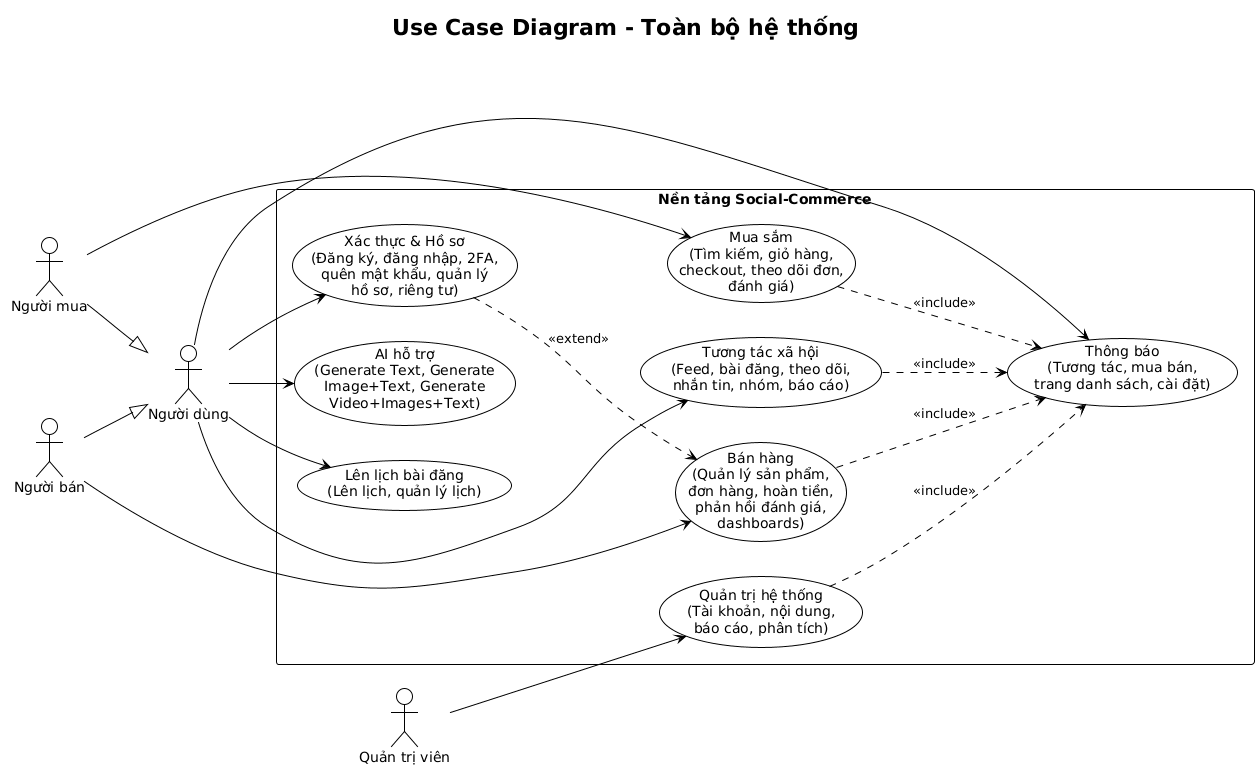
\includegraphics[width=\textwidth]{Images/Usecases/UC-All-System.png}
\caption{Sơ đồ Use Case tổng quan cho toàn hệ thống Social Commerce}
\label{fig:usecase-total}
\end{figure}

\subsection{Module 1: Quản lý Người dùng và Xác thực}
\subsubsection{Module 1: Quản lý Người dùng và Xác thực}
Module này bao gồm các chức năng cốt lõi liên quan đến việc tạo lập, xác thực và quản lý tài khoản người dùng trong hệ thống.

\begin{figure}[H]
\centering
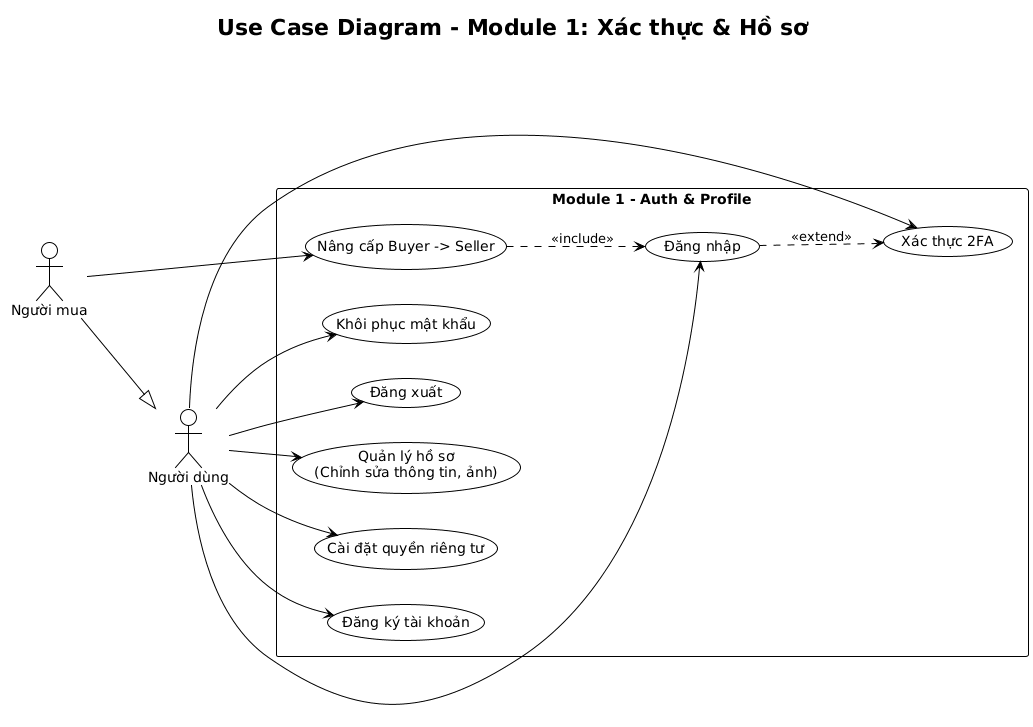
\includegraphics[width=\textwidth]{Images/Usecases/UC-M1-Auth.png}
\caption{Sơ đồ Use Case cho Module 1: Quản lý Người dùng và Xác thực}
\label{fig:usecase-module1}
\end{figure}

% Cấu hình giãn dòng cho bảng dễ đọc hơn
\renewcommand{\arraystretch}{1.3}

% =====================================================
% UC1.1: ĐĂNG KÝ TÀI KHOẢN
% =====================================================
\begin{table}[H]
\centering
\begin{tabularx}{\textwidth}{|l|X|}
\hline
\textbf{Tên Use Case} & \textbf{UC1.1: Đăng ký tài khoản} \\ \hline
\textbf{Tác nhân} & Người dùng chưa đăng nhập \\ \hline
\textbf{Mô tả} & Cho phép người dùng mới tạo một tài khoản trên hệ thống Social Commerce với vai trò mặc định là ``Người mua'' (Buyer). \\ \hline
\textbf{Kích hoạt} & Người dùng nhấn vào nút ``Đăng ký'' trên giao diện. \\ \hline
\textbf{Điều kiện tiên quyết} & 
\begin{itemize}
    \item Người dùng chưa đăng nhập vào hệ thống.
    \item Người dùng có một địa chỉ email hợp lệ và chưa được sử dụng để đăng ký.
\end{itemize} \\ \hline
\textbf{Điều kiện sau} & 
\begin{itemize}
    \item Tài khoản mới được tạo với trạng thái ``chưa xác thực''.
    \item Vai trò người dùng được gán là Buyer.
    \item Hệ thống gửi email/tin nhắn xác thực tài khoản.
    \item Người dùng được chuyển hướng đến trang yêu cầu xác thực.
\end{itemize} \\ \hline
\textbf{Luồng sự kiện chính} & 
\begin{enumerate}
    \item Người dùng truy cập trang Đăng ký.
    \item Người dùng nhập các thông tin bắt buộc.
    \item Người dùng nhấn nút ``Đăng ký''.
    \item Hệ thống kiểm tra tính hợp lệ của dữ liệu.
    \item Hệ thống kiểm tra email đã tồn tại hay chưa.
    \item Hệ thống tạo người dùng mới với trạng thái ``chưa xác thực''.
    \item Hệ thống gửi email/SMS xác thực.
    \item Hệ thống hiển thị thông báo thành công và yêu cầu xác thực.
\end{enumerate} \\ \hline
\textbf{Ngoại lệ} & 
\begin{itemize}
    \item E1: Email không hợp lệ $\rightarrow$ Báo lỗi ``Định dạng email không hợp lệ''.
    \item E2: Mật khẩu xác nhận không khớp $\rightarrow$ Báo lỗi ``Mật khẩu xác nhận không khớp''.
    \item E3: Email đã tồn tại $\rightarrow$ Báo lỗi ``Email này đã được sử dụng''.
    \item E4: Lỗi gửi email $\rightarrow$ Báo lỗi và đề nghị thử lại.
\end{itemize} \\ \hline
\textbf{Ghi chú} & Đây là bước đầu tiên để tham gia vào hệ sinh thái Social Commerce. \\ \hline
\end{tabularx}
\caption{Đặc tả Use Case Đăng ký tài khoản}
\end{table}

% =====================================================
% UC1.2: ĐĂNG NHẬP
% =====================================================
\begin{table}[H]
\centering
\begin{tabularx}{\textwidth}{|l|X|}
\hline
\textbf{Tên Use Case} & \textbf{UC1.2: Đăng nhập vào hệ thống} \\ \hline
\textbf{Tác nhân} & Người dùng chưa đăng nhập \\ \hline
\textbf{Mô tả} & Cho phép người dùng đã có tài khoản truy cập vào hệ thống bằng email và mật khẩu. \\ \hline
\textbf{Kích hoạt} & Người dùng nhấn vào nút ``Đăng nhập'' sau khi điền thông tin. \\ \hline
\textbf{Điều kiện tiên quyết} & Người dùng có một tài khoản đã đăng ký và xác thực. \\ \hline
\textbf{Điều kiện sau} & 
\begin{itemize}
    \item Hệ thống tạo một phiên làm việc (session) cho người dùng.
    \item Hệ thống cấp một JSON Web Token (JWT) để xác thực.
    \item Người dùng được chuyển hướng đến trang chủ.
\end{itemize} \\ \hline
\textbf{Luồng sự kiện chính} & 
\begin{enumerate}
    \item Người dùng truy cập trang Đăng nhập.
    \item Người dùng nhập email và mật khẩu.
    \item Người dùng nhấn nút ``Đăng nhập''.
    \item Hệ thống xác thực thông tin.
    \item Nếu thông tin chính xác và tài khoản không bật 2FA, hệ thống tạo JWT và chuyển hướng người dùng.
\end{enumerate} \\ \hline
\textbf{Ngoại lệ} & 
\begin{itemize}
    \item E1: Sai email hoặc mật khẩu $\rightarrow$ Báo lỗi ``Thông tin đăng nhập không chính xác''.
    \item E2: Tài khoản chưa được xác thực $\rightarrow$ Báo lỗi và yêu cầu xác thực.
    \item E3: Tài khoản bị khóa $\rightarrow$ Báo lỗi ``Tài khoản của bạn đã bị khóa''.
\end{itemize} \\ \hline
\textbf{Ghi chú} & Quá trình xác thực sử dụng JWT để đảm bảo an toàn. \\ \hline
\end{tabularx}
\caption{Đặc tả Use Case Đăng nhập}
\end{table}

% =====================================================
% UC1.3: XÁC THỰC 2 YẾU TỐ (2FA)
% =====================================================
\begin{table}[H]
\centering
\begin{tabularx}{\textwidth}{|l|X|}
\hline
\textbf{Tên Use Case} & \textbf{UC1.3: Sử dụng xác thực hai yếu tố (2FA)} \\ \hline
\textbf{Tác nhân} & Người dùng \\ \hline
\textbf{Mô tả} & Cung cấp một lớp bảo mật bổ sung khi đăng nhập bằng mã xác thực tạm thời. \\ \hline
\textbf{Kích hoạt} & Người dùng có bật 2FA và vừa nhập đúng mật khẩu ở bước đăng nhập. \\ \hline
\textbf{Điều kiện tiên quyết} & 
\begin{itemize}
    \item Người dùng đã kích hoạt tính năng 2FA.
    \item Người dùng đã nhập chính xác email và mật khẩu.
\end{itemize} \\ \hline
\textbf{Điều kiện sau} & 
\begin{itemize}
    \item Danh tính người dùng được xác thực hoàn toàn.
    \item Người dùng được đăng nhập thành công.
\end{itemize} \\ \hline
\textbf{Luồng sự kiện chính} & 
\begin{enumerate}
    \item Hệ thống hiển thị trang nhập mã 2FA.
    \item Người dùng lấy mã từ email (hoặc ứng dụng Authenticator).
    \item Người dùng nhập mã 2FA.
    \item Người dùng nhấn ``Xác nhận''.
    \item Hệ thống kiểm tra mã.
    \item Nếu mã hợp lệ, quá trình đăng nhập hoàn tất.
\end{enumerate} \\ \hline
\textbf{Ngoại lệ} & 
\begin{itemize}
    \item E1: Nhập sai mã 2FA $\rightarrow$ Báo lỗi ``Mã xác thực không chính xác''.
    \item E2: Mã 2FA hết hạn $\rightarrow$ Báo lỗi và yêu cầu thử lại.
\end{itemize} \\ \hline
\textbf{Ghi chú} & Tính năng này tùy chọn và quan trọng cho tài khoản người bán. \\ \hline
\end{tabularx}
\caption{Đặc tả Use Case Xác thực 2FA}
\end{table}

% =====================================================
% UC1.4: KHÔI PHỤC MẬT KHẨU
% =====================================================
\begin{table}[H]
\centering
\begin{tabularx}{\textwidth}{|l|X|}
\hline
\textbf{Tên Use Case} & \textbf{UC1.4: Khôi phục mật khẩu} \\ \hline
\textbf{Tác nhân} & Người dùng chưa đăng nhập \\ \hline
\textbf{Mô tả} & Cho phép người dùng đặt lại mật khẩu trong trường hợp họ quên. \\ \hline
\textbf{Kích hoạt} & Người dùng nhấn vào liên kết ``Quên mật khẩu?'' trên trang Đăng nhập. \\ \hline
\textbf{Điều kiện tiên quyết} & 
\begin{itemize}
    \item Người dùng có một tài khoản đã đăng ký.
    \item Người dùng có quyền truy cập vào email đã đăng ký.
\end{itemize} \\ \hline
\textbf{Điều kiện sau} & Mật khẩu của người dùng được cập nhật thành công. \\ \hline
\textbf{Luồng sự kiện chính} & 
\begin{enumerate}
    \item Người dùng nhấn ``Quên mật khẩu?''.
    \item Hệ thống yêu cầu người dùng nhập email.
    \item Người dùng nhập email và nhấn ``Gửi''.
    \item Hệ thống gửi email chứa liên kết hoặc mã OTP.
    \item Người dùng làm theo hướng dẫn trong email.
    \item Hệ thống chuyển hướng đến trang tạo mật khẩu mới.
    \item Người dùng nhập mật khẩu mới và xác nhận.
    \item Người dùng nhấn ``Lưu thay đổi''.
    \item Hệ thống cập nhật mật khẩu và thông báo thành công.
\end{enumerate} \\ \hline
\textbf{Ngoại lệ} & 
\begin{itemize}
    \item E1: Email không tồn tại $\rightarrow$ Hệ thống hiển thị thông báo chung để bảo mật (tránh lộ danh tính user).
    \item E2: Liên kết/mã OTP hết hạn hoặc không hợp lệ $\rightarrow$ Báo lỗi và yêu cầu làm lại.
    \item E3: Mật khẩu mới không khớp $\rightarrow$ Báo lỗi.
\end{itemize} \\ \hline
\end{tabularx}
\caption{Đặc tả Use Case Khôi phục mật khẩu}
\end{table}

% =====================================================
% UC1.5: ĐĂNG XUẤT
% =====================================================
\begin{table}[H]
\centering
\begin{tabularx}{\textwidth}{|l|X|}
\hline
\textbf{Tên Use Case} & \textbf{UC1.5: Đăng xuất} \\ \hline
\textbf{Tác nhân} & Người dùng \\ \hline
\textbf{Mô tả} & Cho phép người dùng kết thúc phiên làm việc hiện tại một cách an toàn. \\ \hline
\textbf{Kích hoạt} & Người dùng nhấn vào nút ``Đăng xuất''. \\ \hline
\textbf{Điều kiện tiên quyết} & Người dùng đang đăng nhập vào hệ thống. \\ \hline
\textbf{Điều kiện sau} & 
\begin{itemize}
    \item Phiên làm việc của người dùng bị hủy.
    \item JWT trên client bị xóa.
    \item Người dùng được chuyển hướng về trang chủ.
\end{itemize} \\ \hline
\textbf{Luồng sự kiện chính} & 
\begin{enumerate}
    \item Người dùng nhấn nút ``Đăng xuất''.
    \item Hệ thống hủy phiên làm việc và xóa token lưu trữ ở client.
    \item Hệ thống chuyển hướng người dùng về trang chủ.
\end{enumerate} \\ \hline
\end{tabularx}
\caption{Đặc tả Use Case Đăng xuất}
\end{table}

% =====================================================
% UC1.6: QUẢN LÝ HỒ SƠ CÁ NHÂN
% =====================================================
\begin{table}[H]
\centering
\begin{tabularx}{\textwidth}{|l|X|}
\hline
\textbf{Tên Use Case} & \textbf{UC1.6: Quản lý hồ sơ cá nhân} \\ \hline
\textbf{Tác nhân} & Người dùng \\ \hline
\textbf{Mô tả} & Cho phép người dùng xem và chỉnh sửa thông tin cá nhân, ảnh đại diện và ảnh bìa. \\ \hline
\textbf{Kích hoạt} & Người dùng truy cập trang cá nhân và chọn chức năng chỉnh sửa. \\ \hline
\textbf{Điều kiện tiên quyết} & Người dùng đang đăng nhập vào hệ thống. \\ \hline
\textbf{Điều kiện sau} & 
\begin{itemize}
    \item Thông tin cá nhân của người dùng được cập nhật.
    \item Thay đổi được hiển thị ngay lập tức.
\end{itemize} \\ \hline
\textbf{Luồng sự kiện chính} & 
\begin{enumerate}
    \item Người dùng vào trang hồ sơ cá nhân.
    \item Người dùng nhấn ``Chỉnh sửa hồ sơ''.
    \item Người dùng thay đổi thông tin.
    \item Người dùng nhấn ``Lưu thay đổi''.
    \item Hệ thống xác thực và cập nhật dữ liệu.
    \item Hệ thống hiển thị thông báo thành công.
\end{enumerate} \\ \hline
\textbf{Luồng thay thế} & A1: Người dùng nhấn ``Hủy'' $\rightarrow$ Các thay đổi sẽ không được lưu. \\ \hline
\textbf{Ngoại lệ} & 
\begin{itemize}
    \item E1: Lỗi tải lên hình ảnh $\rightarrow$ Báo lỗi tương ứng.
    \item E2: Dữ liệu nhập không hợp lệ $\rightarrow$ Báo lỗi tại trường dữ liệu đó.
\end{itemize} \\ \hline
\textbf{Ghi chú} & Giao diện quản lý cần trực quan và dễ sử dụng. \\ \hline
\end{tabularx}
\caption{Đặc tả Use Case Quản lý hồ sơ}
\end{table}

% =====================================================
% UC1.7: CÀI ĐẶT QUYỀN RIÊNG TƯ
% =====================================================
\begin{table}[H]
\centering
\begin{tabularx}{\textwidth}{|l|X|}
\hline
\textbf{Tên Use Case} & \textbf{UC1.7: Cài đặt quyền riêng tư cho tài khoản} \\ \hline
\textbf{Tác nhân} & Người dùng \\ \hline
\textbf{Mô tả} & Cho phép người dùng tùy chỉnh ai có thể xem hồ sơ, bài đăng hoặc danh sách người theo dõi. \\ \hline
\textbf{Kích hoạt} & Người dùng truy cập vào mục ``Cài đặt \& Quyền riêng tư''. \\ \hline
\textbf{Điều kiện tiên quyết} & Người dùng đang đăng nhập vào hệ thống. \\ \hline
\textbf{Điều kiện sau} & Các thiết lập quyền riêng tư của người dùng được cập nhật. \\ \hline
\textbf{Luồng sự kiện chính} & 
\begin{enumerate}
    \item Người dùng vào trang ``Cài đặt''.
    \item Người dùng chọn tab ``Quyền riêng tư''100.
    \item Người dùng thay đổi các tùy chọn.
    \item Người dùng nhấn ``Lưu thay đổi''.
    \item Hệ thống cập nhật và hiển thị thông báo thành công.
\end{enumerate} \\ \hline
\textbf{Ghi chú} & Tính năng này quan trọng để người dùng cảm thấy an toàn và kiểm soát thông tin. \\ \hline
\end{tabularx}
\caption{Đặc tả Use Case Cài đặt quyền riêng tư}
\end{table}

% =====================================================
% UC1.8: ĐĂNG KÝ NGƯỜI BÁN
% =====================================================
\begin{table}[H]
\centering
\begin{tabularx}{\textwidth}{|l|X|}
\hline
\textbf{Tên Use Case} & \textbf{UC1.8: Đăng ký trở thành Người bán} \\ \hline
\textbf{Tác nhân} & Người dùng (với vai trò Buyer) \\ \hline
\textbf{Mô tả} & Cung cấp quy trình để người dùng ``Người mua'' nâng cấp tài khoản thành ``Người bán''. \\ \hline
\textbf{Kích hoạt} & Người dùng nhấn vào nút ``Trở thành người bán''. \\ \hline
\textbf{Điều kiện tiên quyết} & 
\begin{itemize}
    \item Người dùng đang đăng nhập.
    \item Người dùng hiện có vai trò là Buyer.
\end{itemize} \\ \hline
\textbf{Điều kiện sau} & 
\begin{itemize}
    \item Hồ sơ đăng ký Seller được lưu và chuyển sang trạng thái chờ duyệt (\textit{REVIEWING}) sau khi hoàn thành các bước bắt buộc.
    \item Khi Admin phê duyệt, vai trò người dùng được cập nhật thành Seller.
\end{itemize} \\ \hline
\textbf{Luồng sự kiện chính} & 
\begin{enumerate}
    \item Người dùng truy cập trang ``Đăng ký Bán hàng'' và bắt đầu hồ sơ.
    \item Người dùng hoàn thành bước 1 (thông tin cá nhân/định danh).
    \item Người dùng hoàn thành bước 2 (thông tin kinh doanh).
    \item Người dùng hoàn thành bước 3 (thông tin ngân hàng) và nộp hồ sơ.
    \item Hệ thống chuyển hồ sơ sang trạng thái ``Đang xem xét''.
    \item Admin xét duyệt hồ sơ.
    \item Nếu được duyệt, hệ thống cập nhật vai trò thành Seller và gửi thông báo kết quả.
\end{enumerate} \\ \hline
\textbf{Luồng thay thế} & A1: Người dùng hủy bỏ quá trình đăng ký. \\ \hline
\textbf{Ngoại lệ} & 
\begin{itemize}
    \item E1: Thông tin ở bất kỳ bước nào không hợp lệ $\rightarrow$ Báo lỗi và yêu cầu sửa.
    \item E2: Hồ sơ bị từ chối $\rightarrow$ Hiển thị lý do từ chối để người dùng bổ sung.
\end{itemize} \\ \hline
\textbf{Ghi chú} & Đây là use case cốt lõi thể hiện mô hình ``buyer-to-seller'' của dự án. \\ \hline
\end{tabularx}
\caption{Đặc tả Use Case Đăng ký làm Người bán}
\end{table}

\subsection{Module 2: Tương tác Xã hội}
\subsubsection{Module 2: Tương tác Xã hội}
Module này tập trung vào các tính năng kết nối cộng đồng, chia sẻ nội dung và tương tác giữa người mua và người bán, tạo tiền đề cho các hoạt động thương mại.

\begin{figure}[H]
\centering
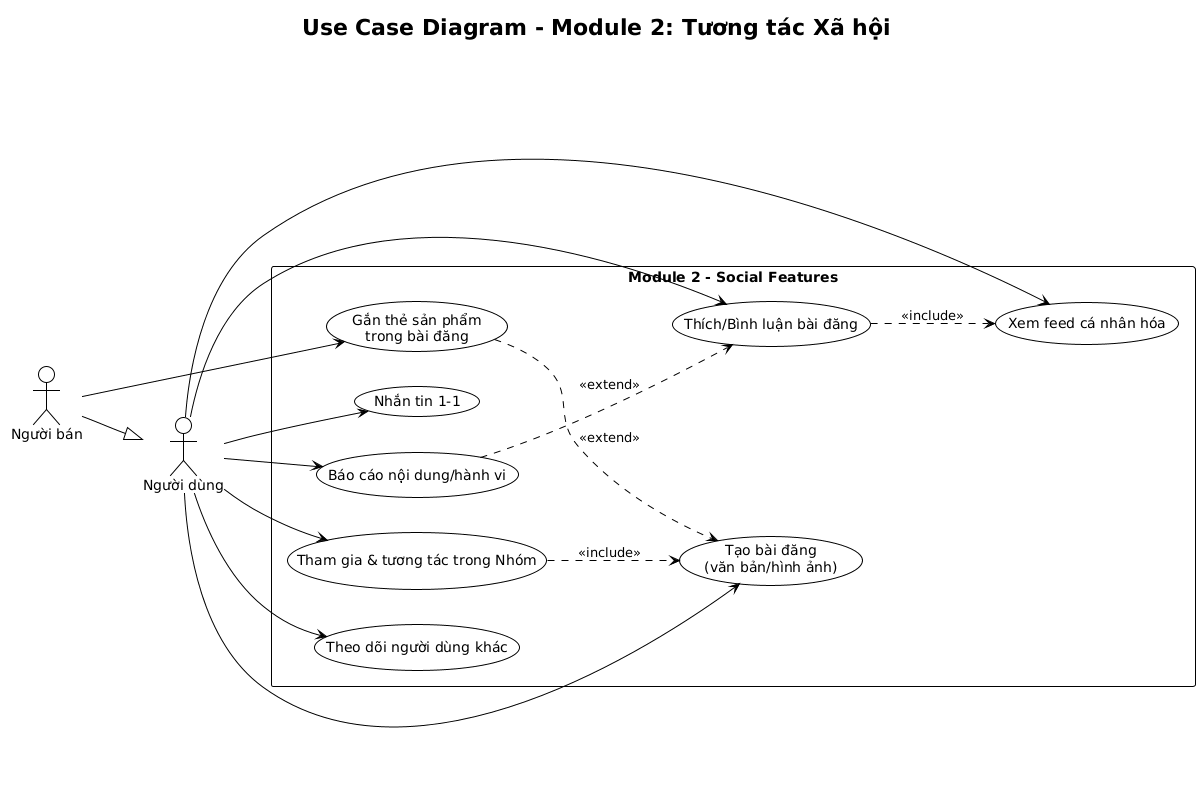
\includegraphics[width=\textwidth]{Images/Usecases/UC-M2-Social.png}
\caption{Sơ đồ Use Case cho Module 2: Tương tác Xã hội}
\label{fig:usecase-module2}
\end{figure}

% Cấu hình giãn dòng
\renewcommand{\arraystretch}{1.3}

% =====================================================
% UC2.1: XEM BẢNG TIN
% =====================================================
\begin{table}[H]
\centering
\begin{tabularx}{\textwidth}{|l|X|}
\hline
\textbf{Tên Use Case} & \textbf{UC2.1: Xem bảng tin (Feed) cá nhân hóa} \\ \hline
\textbf{Tác nhân} & Người dùng \\ \hline
\textbf{Mô tả} & Hiển thị một Bảng tin (Feed) được cá nhân hóa cho người dùng, ưu tiên hiển thị các bài đăng từ những người họ theo dõi và các bài viết có tương tác cao. \\ \hline
\textbf{Kích hoạt} & Người dùng truy cập vào trang chủ sau khi đăng nhập. \\ \hline
\textbf{Điều kiện tiên quyết} & Người dùng đã đăng nhập vào hệ thống. \\ \hline
\textbf{Điều kiện sau} & Người dùng xem được danh sách các bài đăng mới nhất và phù hợp nhất. \\ \hline
\textbf{Luồng sự kiện chính} & 
\begin{enumerate}
    \item Người dùng đăng nhập thành công và được chuyển hướng đến trang chủ.
    \item Hệ thống truy vấn cơ sở dữ liệu để lấy danh sách bài đăng từ những người dùng mà họ đang theo dõi.
    \item Hệ thống cũng lấy các bài đăng có mức độ tương tác cao hoặc được gợi ý.
    \item Hệ thống sắp xếp các bài đăng theo thuật toán (ví dụ: mới nhất, tương tác cao nhất) và hiển thị cho người dùng.
    \item Khi người dùng cuộn trang, hệ thống sẽ tải thêm các bài đăng cũ hơn (infinite scroll).
\end{enumerate} \\ \hline
\textbf{Ngoại lệ} & E1: Lỗi tải dữ liệu $\rightarrow$ Hệ thống hiển thị thông báo lỗi và nút ``Thử lại''. \\ \hline
\textbf{Ghi chú} & Thuật toán sắp xếp feed có thể được cải tiến trong tương lai để tăng tính cá nhân hóa. \\ \hline
\end{tabularx}
\caption{Đặc tả Use Case Xem Bảng tin}
\end{table}

% =====================================================
% UC2.2: TẠO BÀI ĐĂNG
% =====================================================
\begin{table}[H]
\centering
\begin{tabularx}{\textwidth}{|l|X|}
\hline
\textbf{Tên Use Case} & \textbf{UC2.2: Tạo bài đăng (văn bản, hình ảnh)} \\ \hline
\textbf{Tác nhân} & Người dùng \\ \hline
\textbf{Mô tả} & Cho phép người dùng tạo và chia sẻ các bài đăng với nội dung văn bản và hình ảnh lên trang cá nhân của họ và Bảng tin của những người theo dõi. \\ \hline
\textbf{Kích hoạt} & Người dùng nhấn vào nút ``Tạo bài đăng'' trên giao diện. \\ \hline
\textbf{Điều kiện tiên quyết} & Người dùng đã đăng nhập vào hệ thống. \\ \hline
\textbf{Điều kiện sau} & 
\begin{itemize}
    \item Một bài đăng mới được tạo và lưu vào cơ sở dữ liệu.
    \item Bài đăng mới xuất hiện trên trang cá nhân của người dùng và Bảng tin của những người theo dõi.
\end{itemize} \\ \hline
\textbf{Luồng sự kiện chính} & 
\begin{enumerate}
    \item Người dùng nhấn vào ô tạo bài đăng.
    \item Người dùng nhập nội dung văn bản.
    \item Người dùng tùy chọn tải lên một hoặc nhiều hình ảnh.
    \item Người dùng nhấn nút ``Đăng''.
    \item Hệ thống kiểm tra tính hợp lệ của nội dung.
    \item Hệ thống lưu bài đăng vào cơ sở dữ liệu.
    \item Hệ thống hiển thị bài đăng mới ngay trên giao diện của người dùng.
\end{enumerate} \\ \hline
\textbf{Luồng thay thế} & A1: Người dùng hủy bỏ việc tạo bài đăng, nội dung nháp sẽ bị xóa. \\ \hline
\textbf{Ngoại lệ} & 
\begin{itemize}
    \item E1: Lỗi tải lên hình ảnh (kích thước quá lớn, định dạng không hỗ trợ) $\rightarrow$ Hệ thống báo lỗi.
    \item E2: Mất kết nối mạng khi đang đăng bài $\rightarrow$ Hệ thống báo lỗi và lưu lại nội dung nháp (nếu có thể).
\end{itemize} \\ \hline
\end{tabularx}
\caption{Đặc tả Use Case Tạo bài đăng}
\end{table}

% =====================================================
% UC2.3: GẮN THẺ SẢN PHẨM (QUAN TRỌNG)
% =====================================================
\begin{table}[H]
\centering
\begin{tabularx}{\textwidth}{|l|X|}
\hline
\textbf{Tên Use Case} & \textbf{UC2.3: Gắn thẻ sản phẩm vào bài đăng} \\ \hline
\textbf{Tác nhân} & Người bán (Seller) \\ \hline
\textbf{Mô tả} & Cho phép người dùng ``Người bán'' gắn thẻ các sản phẩm từ cửa hàng của mình trực tiếp vào bài đăng, giúp người xem dễ dàng khám phá và mua sản phẩm. \\ \hline
\textbf{Kích hoạt} & Người bán nhấn vào tùy chọn ``Gắn thẻ sản phẩm'' khi đang tạo bài đăng. \\ \hline
\textbf{Điều kiện tiên quyết} & 
\begin{itemize}
    \item Người dùng đã đăng nhập với vai trò Seller.
    \item Người dùng đang trong quá trình tạo hoặc chỉnh sửa một bài đăng.
    \item Người bán đã có ít nhất một sản phẩm trong cửa hàng.
\end{itemize} \\ \hline
\textbf{Điều kiện sau} & Bài đăng được tạo ra có chứa liên kết trực tiếp đến trang sản phẩm đã được gắn thẻ. \\ \hline
\textbf{Luồng sự kiện chính} & 
\begin{enumerate}
    \item Khi đang soạn bài đăng, người bán chọn chức năng ``Gắn thẻ sản phẩm''.
    \item Hệ thống hiển thị danh sách sản phẩm của người bán.
    \item Người bán chọn một sản phẩm để gắn thẻ.
    \item Người bán hoàn tất việc tạo bài đăng và nhấn ``Đăng''.
    \item Hệ thống lưu bài đăng cùng danh sách \texttt{productTags} đã chọn (đa sản phẩm, đa vị trí neo).
    \item Khi hiển thị, bài đăng có thẻ sản phẩm để điều hướng sang trang chi tiết.
\end{enumerate} \\ \hline
\textbf{Ngoại lệ} & E1: Người bán cố gắng gắn thẻ một sản phẩm đã bị xóa hoặc ẩn $\rightarrow$ Hệ thống báo lỗi. \\ \hline
\textbf{Ghi chú} & Đây là tính năng kết nối trực tiếp giữa hoạt động xã hội và thương mại. \\ \hline
\end{tabularx}
\caption{Đặc tả Use Case Gắn thẻ sản phẩm}
\end{table}

% =====================================================
% UC2.4: TƯƠNG TÁC (LIKE/COMMENT)
% =====================================================
\begin{table}[H]
\centering
\begin{tabularx}{\textwidth}{|l|X|}
\hline
\textbf{Tên Use Case} & \textbf{UC2.4: Tương tác với bài đăng} \\ \hline
\textbf{Tác nhân} & Người dùng \\ \hline
\textbf{Mô tả} & Cho phép người dùng thể hiện sự quan tâm hoặc thảo luận về một bài đăng bằng cách nhấn ``Thích'' (Like) hoặc để lại ``Bình luận'' (Comment). \\ \hline
\textbf{Kích hoạt} & Người dùng nhấn vào nút ``Thích'' hoặc ô ``Bình luận'' bên dưới một bài đăng. \\ \hline
\textbf{Điều kiện tiên quyết} & Người dùng đã đăng nhập vào hệ thống. \\ \hline
\textbf{Điều kiện sau} & 
\begin{itemize}
    \item Khi Thích: Lượt thích của bài đăng được tăng lên (hoặc bỏ thích nếu nhấn lại).
    \item Khi Bình luận: Một bình luận mới được thêm vào bài đăng và hiển thị cho người dùng khác.
\end{itemize} \\ \hline
\textbf{Luồng sự kiện chính} & 
\begin{itemize}
    \item \textbf{Thích bài đăng:}
    \begin{enumerate}
        \item Người dùng nhấn vào biểu tượng ``Thích''.
        \item Hệ thống cập nhật số lượt thích và lưu trạng thái ``đã thích'' của người dùng.
    \end{enumerate}
    \item \textbf{Bình luận bài đăng:}
    \begin{enumerate}
        \item Người dùng nhấn vào ô bình luận.
        \item Người dùng nhập nội dung và nhấn gửi.
        \item Hệ thống lưu bình luận và hiển thị nó bên dưới bài đăng.
    \end{enumerate}
\end{itemize} \\ \hline
\textbf{Ngoại lệ} & E1: Mất kết nối mạng $\rightarrow$ Hệ thống báo lỗi, hành động không thực hiện. \\ \hline
\end{tabularx}
\caption{Đặc tả Use Case Tương tác bài đăng}
\end{table}

% =====================================================
% UC2.5: THEO DÕI NGƯỜI DÙNG
% =====================================================
\begin{table}[H]
\centering
\begin{tabularx}{\textwidth}{|l|X|}
\hline
\textbf{Tên Use Case} & \textbf{UC2.5: Theo dõi người dùng khác} \\ \hline
\textbf{Tác nhân} & Người dùng \\ \hline
\textbf{Mô tả} & Cho phép người dùng theo dõi (follow) một người dùng khác để xem các bài đăng của họ trên Bảng tin cá nhân. \\ \hline
\textbf{Kích hoạt} & Người dùng nhấn vào nút ``Theo dõi'' trên trang cá nhân của một người dùng khác. \\ \hline
\textbf{Điều kiện tiên quyết} & Người dùng đã đăng nhập vào hệ thống. \\ \hline
\textbf{Điều kiện sau} & 
\begin{itemize}
    \item Một mối quan hệ ``theo dõi'' được thiết lập.
    \item Các bài đăng trong tương lai của người bị theo dõi sẽ xuất hiện trên Bảng tin của người theo dõi.
\end{itemize} \\ \hline
\textbf{Luồng sự kiện chính} & 
\begin{enumerate}
    \item Người dùng truy cập trang cá nhân của một người khác.
    \item Người dùng nhấn nút ``Theo dõi''.
    \item Hệ thống ghi nhận mối quan hệ theo dõi vào cơ sở dữ liệu.
    \item Nút ``Theo dõi'' chuyển thành ``Đang theo dõi''.
\end{enumerate} \\ \hline
\textbf{Luồng thay thế} & A1: Người dùng nhấn nút ``Hủy theo dõi'' để xóa bỏ mối quan hệ. \\ \hline
\textbf{Ngoại lệ} & E1: Người dùng cố gắng theo dõi chính mình $\rightarrow$ Hệ thống không cho phép. \\ \hline
\end{tabularx}
\caption{Đặc tả Use Case Theo dõi}
\end{table}

% =====================================================
% UC2.6: NHẮN TIN 1-1 (REAL-TIME)
% =====================================================
\begin{table}[H]
\centering
\begin{tabularx}{\textwidth}{|l|X|}
\hline
\textbf{Tên Use Case} & \textbf{UC2.6: Nhắn tin 1-1} \\ \hline
\textbf{Tác nhân} & Người dùng \\ \hline
\textbf{Mô tả} & Cung cấp hệ thống chat thời gian thực cho phép người dùng nhắn tin trực tiếp với nhau, tạo điều kiện cho người mua và người bán trao đổi về sản phẩm. \\ \hline
\textbf{Kích hoạt} & Người dùng nhấn vào nút ``Nhắn tin'' trên trang cá nhân của người khác. \\ \hline
\textbf{Điều kiện tiên quyết} & Người dùng đã đăng nhập vào hệ thống. \\ \hline
\textbf{Điều kiện sau} & 
\begin{itemize}
    \item Tin nhắn được gửi thành công và hiển thị trong cửa sổ chat của cả hai người dùng trong thời gian thực.
    \item Tin nhắn được lưu lại trong lịch sử trò chuyện.
\end{itemize} \\ \hline
\textbf{Luồng sự kiện chính} & 
\begin{enumerate}
    \item Người dùng A mở cuộc hội thoại với người dùng B (tạo mới nếu chưa có).
    \item Người dùng A nhập tin nhắn và nhấn gửi.
    \item Hệ thống lưu tin nhắn vào cơ sở dữ liệu.
    \item Hệ thống phát sự kiện Socket.io theo room hội thoại để cập nhật real-time cho các client đang tham gia.
    \item Nếu người nhận đang offline, hệ thống tạo thông báo để hiển thị khi người nhận quay lại.
\end{enumerate} \\ \hline
\textbf{Ngoại lệ} & 
\begin{itemize}
    \item E1: Người gửi không thuộc cuộc hội thoại $\rightarrow$ Hệ thống từ chối gửi tin nhắn.
    \item E2: Mất kết nối mạng $\rightarrow$ Hệ thống báo lỗi gửi không thành công và cho phép thử lại.
\end{itemize} \\ \hline
\end{tabularx}
\caption{Đặc tả Use Case Nhắn tin}
\end{table}

% =====================================================
% UC2.7: THAM GIA NHÓM
% =====================================================
\begin{table}[H]
\centering
\begin{tabularx}{\textwidth}{|l|X|}
\hline
\textbf{Tên Use Case} & \textbf{UC2.7: Tham gia và tương tác trong Nhóm} \\ \hline
\textbf{Tác nhân} & Người dùng \\ \hline
\textbf{Mô tả} & Cho phép người dùng tham gia vào các Nhóm (Groups) hoặc cộng đồng để thảo luận về những chủ đề chung mà họ quan tâm. \\ \hline
\textbf{Kích hoạt} & Người dùng tìm kiếm và yêu cầu tham gia một nhóm. \\ \hline
\textbf{Điều kiện tiên quyết} & Người dùng đã đăng nhập vào hệ thống. \\ \hline
\textbf{Điều kiện sau} & 
\begin{itemize}
    \item Người dùng trở thành thành viên của nhóm.
    \item Người dùng có thể xem và tạo bài đăng bên trong nhóm đó.
\end{itemize} \\ \hline
\textbf{Luồng sự kiện chính} & 
\begin{enumerate}
    \item Người dùng tìm kiếm hoặc được gợi ý nhóm.
    \item Nhấn ``Tham gia nhóm''.
    \item Nếu nhóm công khai, người dùng trở thành thành viên ngay. Nếu nhóm riêng tư, yêu cầu được gửi để phê duyệt.
    \item Sau khi trở thành thành viên, người dùng có thể tương tác với các nội dung trong nhóm.
\end{enumerate} \\ \hline
\textbf{Luồng thay thế} & A1: Người dùng rời khỏi một nhóm mà họ đã tham gia. \\ \hline
\textbf{Ngoại lệ} & E1: Người dùng bị cấm khỏi nhóm $\rightarrow$ Hệ thống không cho phép tham gia lại. \\ \hline
\end{tabularx}
\caption{Đặc tả Use Case Tham gia Nhóm}
\end{table}

% =====================================================
% UC2.8: BÁO CÁO VI PHẠM
% =====================================================
\begin{table}[H]
\centering
\begin{tabularx}{\textwidth}{|l|X|}
\hline
\textbf{Tên Use Case} & \textbf{UC2.8: Báo cáo nội dung/hành vi vi phạm} \\ \hline
\textbf{Tác nhân} & Người dùng \\ \hline
\textbf{Mô tả} & Cung cấp công cụ để người dùng báo cáo (report) các bài đăng, sản phẩm, hoặc hành vi của người dùng khác mà họ cho là vi phạm. \\ \hline
\textbf{Kích hoạt} & Người dùng nhấn vào tùy chọn ``Báo cáo'' trên một bài đăng, bình luận hoặc trang cá nhân. \\ \hline
\textbf{Điều kiện tiên quyết} & Người dùng đã đăng nhập vào hệ thống. \\ \hline
\textbf{Điều kiện sau} & Một báo cáo được tạo và gửi đến hệ thống quản trị để xem xét. \\ \hline
\textbf{Luồng sự kiện chính} & 
\begin{enumerate}
    \item Người dùng chọn đối tượng cần báo cáo.
    \item Người dùng nhấn vào tùy chọn ``Báo cáo''.
    \item Hệ thống hiển thị biểu mẫu yêu cầu chọn lý do báo cáo.
    \item Người dùng chọn lý do và có thể thêm mô tả chi tiết.
    \item Người dùng nhấn ``Gửi báo cáo''.
    \item Hệ thống ghi nhận báo cáo và thông báo cho người dùng.
\end{enumerate} \\ \hline
\textbf{Ngoại lệ} & E1: Người dùng cố gắng báo cáo cùng một đối tượng nhiều lần trong thời gian ngắn $\rightarrow$ Hệ thống hạn chế để tránh spam. \\ \hline
\textbf{Ghi chú} & Tính năng này giúp duy trì môi trường an toàn và trong sạch cho cộng đồng. \\ \hline
\end{tabularx}
\caption{Đặc tả Use Case Báo cáo vi phạm}
\end{table}

\subsection{Module 3: Hoạt động Thương mại}
\subsubsection{Module 3: Hoạt động Thương mại}
Đây là phân hệ lõi (Core Domain) của hệ thống Social Commerce, nơi diễn ra các hoạt động trao đổi, mua bán hàng hóa giữa các người dùng.

\begin{figure}[H]
\centering
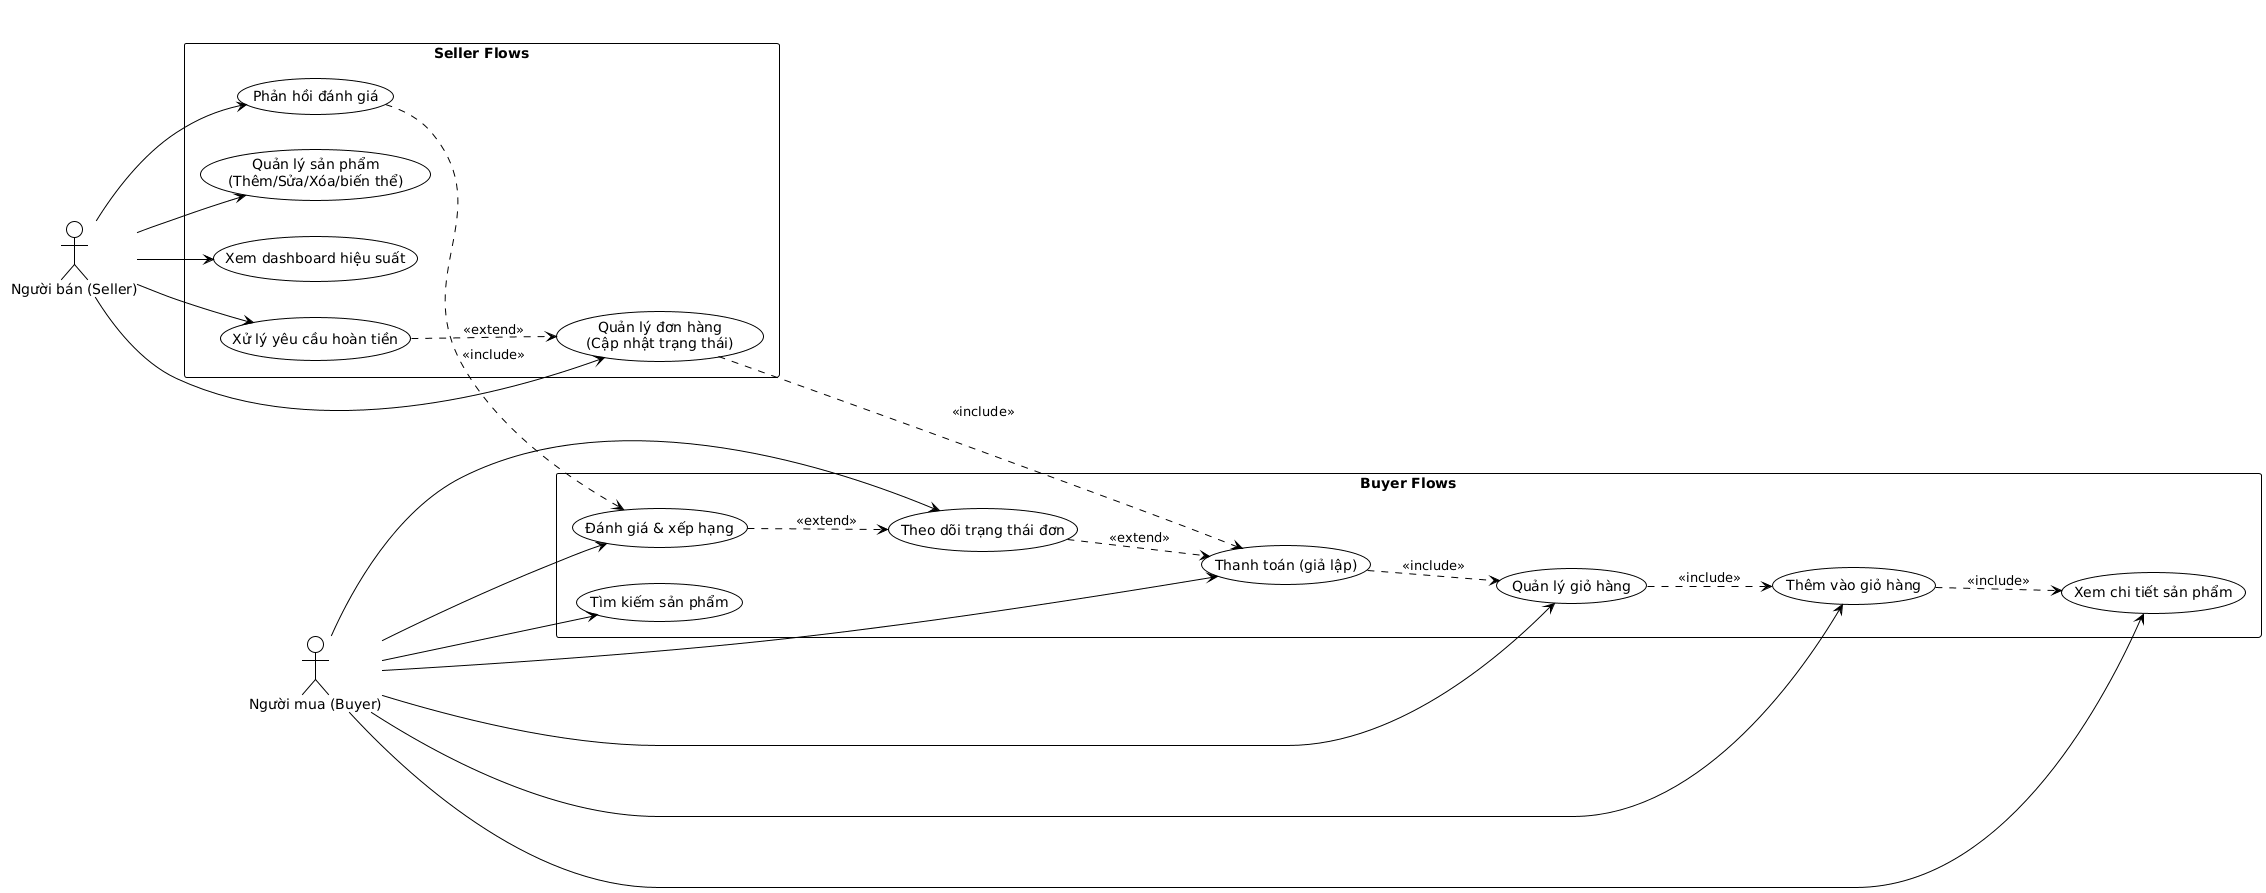
\includegraphics[width=\textwidth]{Images/Usecases/UC-M3-Commerce.png}
\caption{Sơ đồ Use Case cho Module 3: Hoạt động Thương mại}
\label{fig:usecase-module3}
\end{figure}

\renewcommand{\arraystretch}{1.3}

% =====================================================
% PHẦN 1: DÀNH CHO NGƯỜI MUA (BUYER)
% =====================================================
\paragraph{A. Các chức năng dành cho Người mua (Buyer)}

% UC3.1: TÌM KIẾM SẢN PHẨM
\begin{table}[H]
\centering
\begin{tabularx}{\textwidth}{|l|X|}
\hline
\textbf{Tên Use Case} & \textbf{UC3.1: Tìm kiếm sản phẩm} \\ \hline
\textbf{Tác nhân} & Người mua (Buyer) \\ \hline
\textbf{Mô tả} & Cho phép người mua tìm kiếm các sản phẩm họ quan tâm bằng cách sử dụng thanh tìm kiếm và các bộ lọc chi tiết như danh mục và thẻ (tags). \\ \hline
\textbf{Kích hoạt} & Người mua nhập từ khóa vào thanh tìm kiếm hoặc chọn các bộ lọc trên trang sản phẩm. \\ \hline
\textbf{Điều kiện tiên quyết} & Người mua có thể đã đăng nhập hoặc chưa. \\ \hline
\textbf{Điều kiện sau} & Một danh sách các sản phẩm phù hợp với tiêu chí tìm kiếm được hiển thị cho người mua. \\ \hline
\textbf{Luồng sự kiện chính} & 
\begin{enumerate}
    \item Người mua truy cập trang khám phá sản phẩm.
    \item Người mua nhập từ khóa vào thanh tìm kiếm.
    \item Người mua tùy chọn áp dụng các bộ lọc.
    \item Hệ thống truy vấn cơ sở dữ liệu và trả về danh sách sản phẩm khớp.
    \item Giao diện hiển thị kết quả tìm kiếm cho người mua.
\end{enumerate} \\ \hline
\textbf{Ngoại lệ} & E1: Không tìm thấy sản phẩm nào $\rightarrow$ Hệ thống hiển thị thông báo ``Không tìm thấy kết quả phù hợp''. \\ \hline
\end{tabularx}
\caption{Đặc tả Use Case Tìm kiếm sản phẩm}
\end{table}

% UC3.2: XEM CHI TIẾT SẢN PHẨM
\begin{table}[H]
\centering
\begin{tabularx}{\textwidth}{|l|X|}
\hline
\textbf{Tên Use Case} & \textbf{UC3.2: Xem chi tiết sản phẩm} \\ \hline
\textbf{Tác nhân} & Người mua \\ \hline
\textbf{Mô tả} & Cho phép người mua xem thông tin chi tiết về một sản phẩm, bao gồm hình ảnh, mô tả, giá, các biến thể, thông tin người bán và các đánh giá. \\ \hline
\textbf{Kích hoạt} & Người mua nhấp vào một sản phẩm từ kết quả tìm kiếm, Bảng tin hoặc bất kỳ đâu trên nền tảng. \\ \hline
\textbf{Điều kiện tiên quyết} & Sản phẩm phải tồn tại và đang được bán. \\ \hline
\textbf{Điều kiện sau} & Người mua nắm được đầy đủ thông tin về sản phẩm để ra quyết định mua hàng. \\ \hline
\textbf{Luồng sự kiện chính} & 
\begin{enumerate}
    \item Người mua nhấp vào một sản phẩm.
    \item Hệ thống tải và hiển thị trang chi tiết sản phẩm với đầy đủ thông tin.
    \item Người mua có thể xem các hình ảnh, chọn các biến thể (nếu có) và đọc các đánh giá.
\end{enumerate} \\ \hline
\textbf{Ngoại lệ} & E1: Sản phẩm không còn tồn tại hoặc đã bị ẩn $\rightarrow$ Hệ thống hiển thị trang lỗi ``Sản phẩm không tìm thấy''. \\ \hline
\end{tabularx}
\caption{Đặc tả Use Case Xem chi tiết sản phẩm}
\end{table}

% UC3.3: THÊM VÀO GIỎ HÀNG
\begin{table}[H]
\centering
\begin{tabularx}{\textwidth}{|l|X|}
\hline
\textbf{Tên Use Case} & \textbf{UC3.3: Thêm sản phẩm vào giỏ hàng} \\ \hline
\textbf{Tác nhân} & Người mua \\ \hline
\textbf{Mô tả} & Cho phép người mua thêm sản phẩm, bao gồm các biến thể đã chọn, vào giỏ hàng của mình. Người mua có thể thêm sản phẩm từ nhiều cửa hàng khác nhau. \\ \hline
\textbf{Điều kiện tiên quyết} & 
\begin{itemize}
    \item Người mua đã đăng nhập vào hệ thống.
    \item Người mua đã chọn đầy đủ các biến thể bắt buộc của sản phẩm (nếu có).
\end{itemize} \\ \hline
\textbf{Điều kiện sau} & 
\begin{itemize}
    \item Sản phẩm được thêm vào giỏ hàng của người mua.
    \item Biểu tượng giỏ hàng trên giao diện được cập nhật số lượng.
\end{itemize} \\ \hline
\textbf{Luồng sự kiện chính} & 
\begin{enumerate}
    \item Trên trang chi tiết sản phẩm, người mua chọn số lượng và các biến thể mong muốn.
    \item Người mua nhấn ``Thêm vào giỏ hàng''.
    \item Hệ thống xác định biến thể theo \textit{variantId} (hoặc map từ lựa chọn biến thể), kiểm tra trạng thái sản phẩm và tồn kho.
    \item Hệ thống thêm mới hoặc cập nhật cart item tương ứng trong giỏ hàng của người mua.
    \item Hệ thống hiển thị thông báo thành công.
\end{enumerate} \\ \hline
\textbf{Ngoại lệ} & E1: Sản phẩm đã hết hàng $\rightarrow$ Hệ thống báo lỗi và không cho phép thêm vào giỏ. \\ \hline
\end{tabularx}
\caption{Đặc tả Use Case Thêm vào giỏ hàng}
\end{table}

% UC3.4: QUẢN LÝ GIỎ HÀNG
\begin{table}[H]
\centering
\begin{tabularx}{\textwidth}{|l|X|}
\hline
\textbf{Tên Use Case} & \textbf{UC3.4: Quản lý giỏ hàng} \\ \hline
\textbf{Tác nhân} & Người mua \\ \hline
\textbf{Mô tả} & Cho phép người mua xem lại tất cả sản phẩm trong giỏ hàng, cập nhật số lượng, hoặc xóa sản phẩm khỏi giỏ hàng trước khi thanh toán. \\ \hline
\textbf{Kích hoạt} & Người mua nhấp vào biểu tượng giỏ hàng. \\ \hline
\textbf{Điều kiện tiên quyết} & Người mua đã đăng nhập và có ít nhất một sản phẩm trong giỏ hàng. \\ \hline
\textbf{Điều kiện sau} & Giỏ hàng của người mua được cập nhật theo các thay đổi (số lượng, sản phẩm bị xóa). \\ \hline
\textbf{Luồng sự kiện chính} & 
\begin{enumerate}
    \item Người mua truy cập trang giỏ hàng.
    \item Hệ thống hiển thị danh sách các sản phẩm đã thêm.
    \item Người mua có thể: Tăng/giảm số lượng hoặc xóa sản phẩm.
    \item Hệ thống tự động cập nhật lại tổng số tiền.
\end{enumerate} \\ \hline
\textbf{Ngoại lệ} & E1: Cập nhật số lượng vượt quá số lượng tồn kho $\rightarrow$ Hệ thống báo lỗi. \\ \hline
\end{tabularx}
\caption{Đặc tả Use Case Quản lý giỏ hàng}
\end{table}

% UC3.5: THANH TOÁN
\begin{table}[H]
\centering
\begin{tabularx}{\textwidth}{|l|X|}
\hline
\textbf{Tên Use Case} & \textbf{UC3.5: Thực hiện thanh toán} \\ \hline
\textbf{Tác nhân} & Người mua \\ \hline
\textbf{Mô tả} & Cho phép người mua hoàn tất quy trình mua sắm bằng cách cung cấp thông tin giao hàng và thực hiện thanh toán qua một giao diện giả lập. \\ \hline
\textbf{Điều kiện tiên quyết} & 
\begin{itemize}
    \item Người mua đã đăng nhập.
    \item Giỏ hàng có ít nhất một sản phẩm.
\end{itemize} \\ \hline
\textbf{Điều kiện sau} & 
\begin{itemize}
    \item Một đơn hàng mới được tạo trong hệ thống với trạng thái ``PENDING'' và ``paymentStatus=PENDING''.
    \item Giỏ hàng của người mua được làm rỗng.
    \item Người mua được chuyển đến trang xác nhận đơn hàng thành công.
\end{itemize} \\ \hline
\textbf{Luồng sự kiện chính} & 
\begin{enumerate}
    \item Từ giỏ hàng, người mua nhấn ``Thanh toán''.
    \item Hệ thống kiểm tra tồn kho lần cuối cho từng cart item.
    \item Người mua điền thông tin giao hàng.
    \item Người mua chọn phương thức thanh toán (giả lập).
    \item Người mua xác nhận đơn hàng.
    \item Hệ thống tạo bản ghi Order/OrderItem, chốt đơn giá tại thời điểm đặt hàng và trừ tồn kho.
    \item Hệ thống hiển thị thông báo đặt hàng thành công.
\end{enumerate} \\ \hline
\textbf{Ngoại lệ} & E1: Một sản phẩm trong giỏ đã hết hàng $\rightarrow$ Hệ thống báo lỗi và yêu cầu cập nhật giỏ hàng. \\ \hline
\end{tabularx}
\caption{Đặc tả Use Case Thanh toán}
\end{table}

% UC3.6: THEO DÕI ĐƠN HÀNG
\begin{table}[H]
\centering
\begin{tabularx}{\textwidth}{|l|X|}
\hline
\textbf{Tên Use Case} & \textbf{UC3.6: Theo dõi trạng thái đơn hàng} \\ \hline
\textbf{Tác nhân} & Người mua \\ \hline
\textbf{Mô tả} & Cho phép người mua xem danh sách các đơn hàng đã đặt và theo dõi trạng thái hiện tại của chúng (ví dụ: Đang xử lý, Đang giao, Đã giao). \\ \hline
\textbf{Kích hoạt} & Người mua truy cập vào mục ``Đơn hàng của tôi'' trong trang cá nhân. \\ \hline
\textbf{Điều kiện tiên quyết} & Người mua đã đăng nhập và đã đặt ít nhất một đơn hàng. \\ \hline
\textbf{Điều kiện sau} & Người mua biết được tình trạng hiện tại của đơn hàng. \\ \hline
\textbf{Luồng sự kiện chính} & 
\begin{enumerate}
    \item Người mua vào trang quản lý đơn hàng.
    \item Hệ thống hiển thị danh sách tất cả các đơn hàng đã đặt, kèm theo mã đơn hàng, ngày đặt và trạng thái.
    \item Người mua có thể nhấp vào một đơn hàng để xem chi tiết.
\end{enumerate} \\ \hline
\textbf{Ghi chú} & Trạng thái đơn hàng sẽ do Người bán cập nhật (tham chiếu UC3.10). \\ \hline
\end{tabularx}
\caption{Đặc tả Use Case Theo dõi đơn hàng}
\end{table}

% UC3.7: ĐÁNH GIÁ SẢN PHẨM
\begin{table}[H]
\centering
\begin{tabularx}{\textwidth}{|l|X|}
\hline
\textbf{Tên Use Case} & \textbf{UC3.7: Đánh giá và xếp hạng} \\ \hline
\textbf{Tác nhân} & Người mua \\ \hline
\textbf{Mô tả} & Sau khi mua hàng, người mua có thể để lại phản hồi bằng cách viết đánh giá và cho điểm (xếp hạng sao) cho sản phẩm và người bán. \\ \hline
\textbf{Điều kiện tiên quyết} & 
\begin{itemize}
    \item Người mua đã đăng nhập.
    \item Đơn hàng chứa sản phẩm đó phải ở trạng thái ``Đã giao'' hoặc ``Hoàn thành''.
\end{itemize} \\ \hline
\textbf{Điều kiện sau} & 
\begin{itemize}
    \item Một đánh giá mới được lưu vào cơ sở dữ liệu.
    \item Đánh giá và xếp hạng được hiển thị công khai.
\end{itemize} \\ \hline
\textbf{Luồng sự kiện chính} & 
\begin{enumerate}
    \item Người mua vào mục đơn hàng đã giao hoặc hoàn thành.
    \item Người mua chọn sản phẩm muốn đánh giá và nhấn ``Đánh giá''.
    \item Hệ thống hiển thị form đánh giá (chọn sao, viết bình luận, tải ảnh).
    \item Người mua điền thông tin và nhấn ``Gửi đánh giá''.
    \item Hệ thống xác thực quyền theo \textit{orderItemId} và lưu đánh giá.
\end{enumerate} \\ \hline
\textbf{Ngoại lệ} & E1: Người mua cố gắng đánh giá một sản phẩm họ chưa mua hoặc đã đánh giá trước đó $\rightarrow$ Hệ thống không cho phép. \\ \hline
\textbf{Ghi chú} & Đánh giá là một phần quan trọng để xây dựng lòng tin trong cộng đồng. \\ \hline
\end{tabularx}
\caption{Đặc tả Use Case Đánh giá sản phẩm}
\end{table}

\vspace{1cm}

% =====================================================
% PHẦN 2: DÀNH CHO NGƯỜI BÁN (SELLER)
% =====================================================
\paragraph{B. Các chức năng dành cho Người bán (Seller)}

% UC3.8: QUẢN LÝ SẢN PHẨM
\begin{table}[H]
\centering
\begin{tabularx}{\textwidth}{|l|X|}
\hline
\textbf{Tên Use Case} & \textbf{UC3.8: Quản lý sản phẩm} \\ \hline
\textbf{Tác nhân} & Người bán (Seller) \\ \hline
\textbf{Mô tả} & Cung cấp công cụ để người bán thêm, sửa, xóa sản phẩm và quản lý thông tin nâng cao như biến thể (kích cỡ, màu sắc), danh mục và thẻ. \\ \hline
\textbf{Kích hoạt} & Người bán truy cập vào mục ``Quản lý sản phẩm'' trong Bảng điều khiển của mình. \\ \hline
\textbf{Điều kiện tiên quyết} & Người dùng phải đăng nhập với vai trò Seller. \\ \hline
\textbf{Điều kiện sau} & Danh sách sản phẩm của cửa hàng được cập nhật. \\ \hline
\textbf{Luồng sự kiện chính} & 
\begin{enumerate}
    \item Người bán vào trang quản lý sản phẩm và nhấn ``Thêm sản phẩm mới''.
    \item Người bán điền đầy đủ thông tin: tên, mô tả, giá, tồn kho, hình ảnh...
    \item Người bán tùy chọn thêm các biến thể, danh mục, thẻ.
    \item Người bán nhấn ``Lưu''.
    \item Hệ thống xác thực dữ liệu và tạo một bản ghi sản phẩm mới.
    \item Người bán có thể chọn một sản phẩm có sẵn để ``Sửa'' hoặc ``Xóa''.
\end{enumerate} \\ \hline
\textbf{Ngoại lệ} & E1: Dữ liệu nhập vào không hợp lệ (ví dụ: giá âm) $\rightarrow$ Hệ thống báo lỗi. \\ \hline
\textbf{Ghi chú} & Đây là chức năng cốt lõi cho phép người bán đưa hàng hóa lên nền tảng. \\ \hline
\end{tabularx}
\caption{Đặc tả Use Case Quản lý sản phẩm}
\end{table}

% UC3.9: DASHBOARD
\begin{table}[H]
\centering
\begin{tabularx}{\textwidth}{|l|X|}
\hline
\textbf{Tên Use Case} & \textbf{UC3.9: Xem dashboard hiệu suất} \\ \hline
\textbf{Tác nhân} & Người bán \\ \hline
\textbf{Mô tả} & Cung cấp một Bảng điều khiển (dashboard) trực quan để người bán theo dõi hiệu suất kinh doanh qua các chỉ số như lượt xem, doanh số, số đơn hàng... \\ \hline
\textbf{Kích hoạt} & Người bán truy cập vào trang Dashboard chính sau khi đăng nhập. \\ \hline
\textbf{Điều kiện tiên quyết} & Người dùng phải đăng nhập với vai trò Seller. \\ \hline
\textbf{Điều kiện sau} & Người bán nắm được tình hình kinh doanh tổng quan của mình. \\ \hline
\textbf{Luồng sự kiện chính} & 
\begin{enumerate}
    \item Người bán truy cập trang Dashboard.
    \item Hệ thống tổng hợp dữ liệu trong một khoảng thời gian nhất định.
    \item Hệ thống hiển thị dữ liệu dưới dạng các con số, biểu đồ để dễ theo dõi.
    \item Người bán có thể thay đổi khoảng thời gian xem báo cáo.
\end{enumerate} \\ \hline
\textbf{Ghi chú} & Giúp người bán đưa ra các quyết định kinh doanh tốt hơn. \\ \hline
\end{tabularx}
\caption{Đặc tả Use Case Xem Dashboard}
\end{table}

% UC3.10: QUẢN LÝ ĐƠN HÀNG
\begin{table}[H]
\centering
\begin{tabularx}{\textwidth}{|l|X|}
\hline
\textbf{Tên Use Case} & \textbf{UC3.10: Quản lý đơn hàng} \\ \hline
\textbf{Tác nhân} & Người bán \\ \hline
\textbf{Mô tả} & Cho phép người bán xem danh sách các đơn hàng và cập nhật trạng thái của chúng (ví dụ: từ ``Đang xử lý'' sang ``Đang giao''). \\ \hline
\textbf{Kích hoạt} & Người bán truy cập vào mục ``Quản lý đơn hàng'' trong dashboard. \\ \hline
\textbf{Điều kiện tiên quyết} & 
\begin{itemize}
    \item Người dùng phải đăng nhập với vai trò Seller.
    \item Cửa hàng có ít nhất một đơn hàng.
\end{itemize} \\ \hline
\textbf{Điều kiện sau} & Trạng thái của đơn hàng được cập nhật và người mua sẽ thấy được sự thay đổi này. \\ \hline
\textbf{Luồng sự kiện chính} & 
\begin{enumerate}
    \item Người bán vào trang quản lý đơn hàng.
    \item Hệ thống hiển thị danh sách các đơn hàng mới.
    \item Người bán nhấp vào một đơn hàng để xem chi tiết.
    \item Sau khi chuẩn bị xong, người bán thay đổi trạng thái đơn hàng.
    \item Hệ thống lưu lại trạng thái mới.
\end{enumerate} \\ \hline
\end{tabularx}
\caption{Đặc tả Use Case Quản lý đơn hàng của Shop}
\end{table}

% UC3.11: XỬ LÝ HOÀN TIỀN
\begin{table}[H]
\centering
\begin{tabularx}{\textwidth}{|l|X|}
\hline
\textbf{Tên Use Case} & \textbf{UC3.11: Xử lý yêu cầu hoàn tiền} \\ \hline
\textbf{Tác nhân} & Người bán \\ \hline
\textbf{Mô tả} & Cung cấp một quy trình (giả lập) để người bán xem xét và xử lý các yêu cầu hoàn tiền từ người mua. \\ \hline
\textbf{Kích hoạt} & Một người mua gửi yêu cầu hoàn tiền cho một đơn hàng. \\ \hline
\textbf{Điều kiện tiên quyết} & Người dùng phải đăng nhập với vai trò Seller. \\ \hline
\textbf{Điều kiện sau} & Yêu cầu hoàn tiền được giải quyết (chấp nhận hoặc từ chối). \\ \hline
\textbf{Luồng sự kiện chính} & 
\begin{enumerate}
    \item Người bán nhận được thông báo về một yêu cầu hoàn tiền mới.
    \item Người bán vào mục ``Yêu cầu hoàn tiền'' để xem danh sách yêu cầu có trạng thái chờ xử lý.
    \item Người bán đưa ra quyết định ``Chấp nhận'' hoặc ``Từ chối'' yêu cầu.
    \item Nếu chấp nhận, hệ thống cập nhật đơn hàng sang ``REFUNDED''; nếu từ chối, hệ thống lưu lý do từ chối.
    \item Hệ thống ghi nhận quyết định và thông báo lại cho người mua.
    \item Người bán có thể liên hệ với người mua qua tin nhắn để thảo luận thêm.
\end{enumerate} \\ \hline
\textbf{Ghi chú} & Quy trình này được giả lập trong phạm vi đồ án. \\ \hline
\end{tabularx}
\caption{Đặc tả Use Case Xử lý hoàn tiền}
\end{table}

% UC3.12: PHẢN HỒI ĐÁNH GIÁ
\begin{table}[H]
\centering
\begin{tabularx}{\textwidth}{|l|X|}
\hline
\textbf{Tên Use Case} & \textbf{UC3.12: Phản hồi đánh giá} \\ \hline
\textbf{Tác nhân} & Người bán \\ \hline
\textbf{Mô tả} & Cho phép người bán viết phản hồi công khai cho các đánh giá mà người mua đã để lại, giúp tăng cường tương tác và xây dựng niềm tin. \\ \hline
\textbf{Điều kiện tiên quyết} & 
\begin{itemize}
    \item Người dùng phải đăng nhập với vai trò Seller.
    \item Phải có ít nhất một đánh giá từ người mua.
\end{itemize} \\ \hline
\textbf{Điều kiện sau} & Phản hồi của người bán được lưu và hiển thị ngay bên dưới đánh giá của người mua. \\ \hline
\textbf{Luồng sự kiện chính} & 
\begin{enumerate}
    \item Người bán vào mục quản lý đánh giá.
    \item Người bán chọn một đánh giá và nhấn nút ``Phản hồi''.
    \item Người bán nhập nội dung phản hồi và nhấn gửi.
    \item Hệ thống lưu và hiển thị phản hồi đó.
\end{enumerate} \\ \hline
\textbf{Ghi chú} & Đây là một công cụ tốt để thể hiện sự chuyên nghiệp và chăm sóc khách hàng. \\ \hline
\end{tabularx}
\caption{Đặc tả Use Case Phản hồi đánh giá}
\end{table}

\subsection{Module 4: Hệ thống Quản trị}
\subsubsection{Module 4: Hệ thống Quản trị (Admin System)}
Module này cung cấp các công cụ quyền lực cho Quản trị viên (Admin) để giám sát người dùng, kiểm duyệt nội dung và theo dõi sức khỏe của toàn bộ hệ thống.

\begin{figure}[H]
\centering
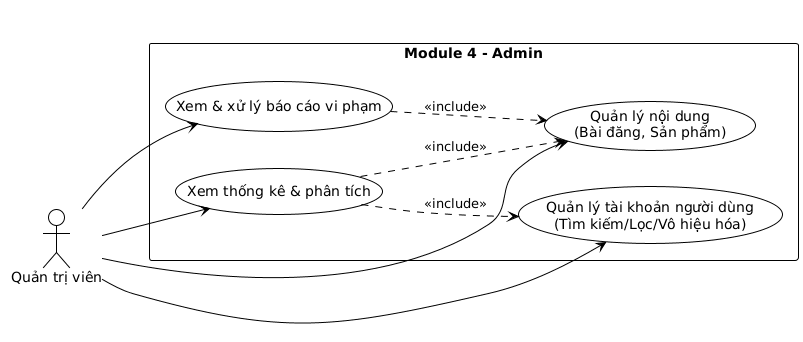
\includegraphics[width=\textwidth]{Images/Usecases/UC-M4-Admin.png}
\caption{Sơ đồ Use Case cho Module 4: Hệ thống Quản trị}
\label{fig:usecase-module4}
\end{figure}

\renewcommand{\arraystretch}{1.3}

% =====================================================
% UC4.1: QUẢN LÝ TÀI KHOẢN NGƯỜI DÙNG
% =====================================================
\begin{table}[H]
\centering
\begin{tabularx}{\textwidth}{|l|X|}
\hline
\textbf{Tên Use Case} & \textbf{UC4.1: Quản lý tài khoản người dùng} \\ \hline
\textbf{Tác nhân} & Quản trị viên (Admin) \\ \hline
\textbf{Mô tả} & Cung cấp cho quản trị viên các công cụ để xem, tìm kiếm, lọc và thực hiện các hành động trên tài khoản người dùng như vô hiệu hóa hoặc cấp lại quyền. \\ \hline
\textbf{Kích hoạt} & Quản trị viên truy cập vào mục ``Quản lý Người dùng'' trong Bảng điều khiển quản trị (Admin Dashboard). \\ \hline
\textbf{Điều kiện tiên quyết} & Quản trị viên đã đăng nhập vào hệ thống với quyền hạn phù hợp. \\ \hline
\textbf{Điều kiện sau} & Thông tin hoặc trạng thái của một hoặc nhiều tài khoản người dùng được thay đổi (ví dụ: tài khoản bị vô hiệu hóa). \\ \hline
\textbf{Luồng sự kiện chính} & 
\begin{enumerate}
    \item Quản trị viên truy cập trang quản lý người dùng.
    \item Hệ thống hiển thị danh sách tất cả người dùng.
    \item Quản trị viên sử dụng các bộ lọc để tìm kiếm người dùng theo tiêu chí.
    \item Quản trị viên chọn một tài khoản người dùng để xem thông tin chi tiết.
    \item Quản trị viên thực hiện một hành động (ví dụ: nhấn nút ``Vô hiệu hóa tài khoản'').
    \item Hệ thống yêu cầu xác nhận hành động.
    \item Quản trị viên xác nhận, và hệ thống cập nhật trạng thái của tài khoản.
\end{enumerate} \\ \hline
\textbf{Ngoại lệ} & 
\begin{itemize}
    \item E1: Quản trị viên cố gắng thực hiện hành động trên tài khoản quản trị viên khác có quyền hạn cao hơn $\rightarrow$ Hệ thống từ chối.
\end{itemize} \\ \hline
\textbf{Ghi chú} & Chức năng này giúp admin duy trì sự kiểm soát đối với cộng đồng người dùng. \\ \hline
\end{tabularx}
\caption{Đặc tả Use Case Quản lý người dùng}
\end{table}

% =====================================================
% UC4.2: QUẢN LÝ NỘI DUNG
% =====================================================
\begin{table}[H]
\centering
\begin{tabularx}{\textwidth}{|l|X|}
\hline
\textbf{Tên Use Case} & \textbf{UC4.2: Quản lý nội dung (Bài đăng/Sản phẩm)} \\ \hline
\textbf{Tác nhân} & Quản trị viên \\ \hline
\textbf{Mô tả} & Cho phép quản trị viên tìm kiếm, xem và xóa các nội dung do người dùng tạo ra như bài đăng hoặc sản phẩm không phù hợp. \\ \hline
\textbf{Kích hoạt} & Quản trị viên truy cập vào các mục quản lý nội dung (ví dụ: ``Quản lý Bài đăng'', ``Quản lý Sản phẩm'') trong dashboard. \\ \hline
\textbf{Điều kiện tiên quyết} & Quản trị viên đã đăng nhập vào hệ thống. \\ \hline
\textbf{Điều kiện sau} & Nội dung không phù hợp (bài đăng, sản phẩm) bị xóa khỏi hệ thống. \\ \hline
\textbf{Luồng sự kiện chính} & 
\begin{enumerate}
    \item Quản trị viên chọn mục nội dung cần quản lý.
    \item Hệ thống hiển thị danh sách các nội dung liên quan.
    \item Quản trị viên sử dụng bộ lọc để tìm kiếm nội dung.
    \item Quản trị viên chọn một nội dung để xem xét.
    \item Nếu nội dung vi phạm, quản trị viên nhấn nút ``Xóa''.
    \item Hệ thống xác nhận và xóa nội dung khỏi cơ sở dữ liệu.
\end{enumerate} \\ \hline
\textbf{Ghi chú} & Việc kiểm duyệt nội dung là cần thiết để giữ cho nền tảng lành mạnh. \\ \hline
\end{tabularx}
\caption{Đặc tả Use Case Quản lý nội dung}
\end{table}

% =====================================================
% UC4.3: XỬ LÝ BÁO CÁO VI PHẠM
% =====================================================
\begin{table}[H]
\centering
\begin{tabularx}{\textwidth}{|l|X|}
\hline
\textbf{Tên Use Case} & \textbf{UC4.3: Xem và xử lý báo cáo vi phạm} \\ \hline
\textbf{Tác nhân} & Quản trị viên \\ \hline
\textbf{Mô tả} & Cho phép quản trị viên xem lại các báo cáo vi phạm được gửi bởi người dùng và đưa ra hành động xử lý phù hợp (ví dụ: xóa nội dung, khóa tài khoản). \\ \hline
\textbf{Điều kiện tiên quyết} & 
\begin{itemize}
    \item Quản trị viên đã đăng nhập vào hệ thống.
    \item Có ít nhất một báo cáo từ người dùng được gửi đến hệ thống.
\end{itemize} \\ \hline
\textbf{Điều kiện sau} & 
\begin{itemize}
    \item Báo cáo được đánh dấu là ``đã xử lý''.
    \item Hành động xử lý đối với nội dung hoặc người dùng bị báo cáo được thực thi.
\end{itemize} \\ \hline
\textbf{Luồng sự kiện chính} & 
\begin{enumerate}
    \item Quản trị viên vào trang quản lý báo cáo.
    \item Hệ thống hiển thị danh sách các báo cáo chưa được xử lý, sắp xếp theo mức độ ưu tiên.
    \item Quản trị viên chọn một báo cáo để xem chi tiết.
    \item Quản trị viên điều hướng đến nội dung/người dùng bị báo cáo để kiểm tra.
    \item Dựa trên kết quả, quản trị viên quyết định hành động (ví dụ: Xóa bài đăng).
    \item Quản trị viên thực hiện hành động thông qua các công cụ quản lý.
    \item Quản trị viên đánh dấu báo cáo là ``Đã xử lý''.
\end{enumerate} \\ \hline
\textbf{Luồng thay thế} & 
\begin{itemize}
    \item A1: Quản trị viên xác định báo cáo là không hợp lệ và đánh dấu là ``Từ chối''.
\end{itemize} \\ \hline
\textbf{Ngoại lệ} & 
\begin{itemize}
    \item E1: Nội dung bị báo cáo đã được người dùng tự xóa trước khi admin xử lý $\rightarrow$ Admin đánh dấu báo cáo là đã giải quyết.
\end{itemize} \\ \hline
\textbf{Ghi chú} & Đây là chức năng tương tác trực tiếp với phản hồi của cộng đồng để duy trì một môi trường an toàn. \\ \hline
\end{tabularx}
\caption{Đặc tả Use Case Xử lý báo cáo}
\end{table}

% =====================================================
% UC4.4: THỐNG KÊ HỆ THỐNG
% =====================================================
\begin{table}[H]
\centering
\begin{tabularx}{\textwidth}{|l|X|}
\hline
\textbf{Tên Use Case} & \textbf{UC4.4: Xem thống kê và phân tích hệ thống} \\ \hline
\textbf{Tác nhân} & Quản trị viên \\ \hline
\textbf{Mô tả} & Cung cấp các biểu đồ và số liệu thống kê trực quan để quản trị viên theo dõi sự phát triển và ``sức khỏe'' của nền tảng. \\ \hline
\textbf{Kích hoạt} & Quản trị viên truy cập vào mục ``Thống kê \& Phân tích'' trong dashboard. \\ \hline
\textbf{Điều kiện tiên quyết} & Quản trị viên đã đăng nhập vào hệ thống. \\ \hline
\textbf{Điều kiện sau} & Quản trị viên nắm được các chỉ số quan trọng về hoạt động của hệ thống để đưa ra quyết định vận hành. \\ \hline
\textbf{Luồng sự kiện chính} & 
\begin{enumerate}
    \item Quản trị viên truy cập trang thống kê.
    \item Hệ thống truy vấn và tổng hợp dữ liệu.
    \item Hệ thống hiển thị các thông tin tổng quan (tổng số người dùng, sản phẩm, bài đăng).
    \item Hệ thống hiển thị các biểu đồ trực quan, chẳng hạn như: Biểu đồ đường thể hiện số lượng người dùng mới; Biểu đồ tròn thể hiện tỷ lệ giữa người mua và người bán.
    \item Quản trị viên có thể thay đổi khoảng thời gian xem thống kê (ví dụ: 7 ngày qua, 30 ngày qua).
\end{enumerate} \\ \hline
\textbf{Ngoại lệ} & 
\begin{itemize}
    \item E1: Lỗi khi tổng hợp dữ liệu $\rightarrow$ Hệ thống báo lỗi.
\end{itemize} \\ \hline
\textbf{Ghi chú} & Các công cụ phân tích này rất quan trọng để theo dõi sự tăng trưởng của hệ thống. \\ \hline
\end{tabularx}
\caption{Đặc tả Use Case Thống kê hệ thống}
\end{table}

\subsection{Module 5: Tích hợp AI Hỗ trợ Sáng tạo Nội dung}
\subsubsection{Module 5: Tích hợp AI Hỗ trợ Sáng tạo}
Đây là tính năng điểm nhấn của dự án, sử dụng Google Gemini API để hỗ trợ người dùng và người bán tạo nội dung đa phương thức chất lượng cao một cách tự động, bao gồm văn bản, hình ảnh và video ngắn. Hệ thống áp dụng pipeline \textbf{Evaluate--Refine Loop}: sau khi gọi API tạo nội dung, kết quả được đánh giá tự động theo các tiêu chí chất lượng (thang điểm 1--10, ngưỡng chấp nhận $\geq$ 7.0). Nếu chưa đạt, hệ thống tự động sửa prompt và thử lại (tối đa 3 lần) trước khi trả kết quả tốt nhất kèm gợi ý chỉnh sửa cho người dùng.

\begin{figure}[H]
\centering
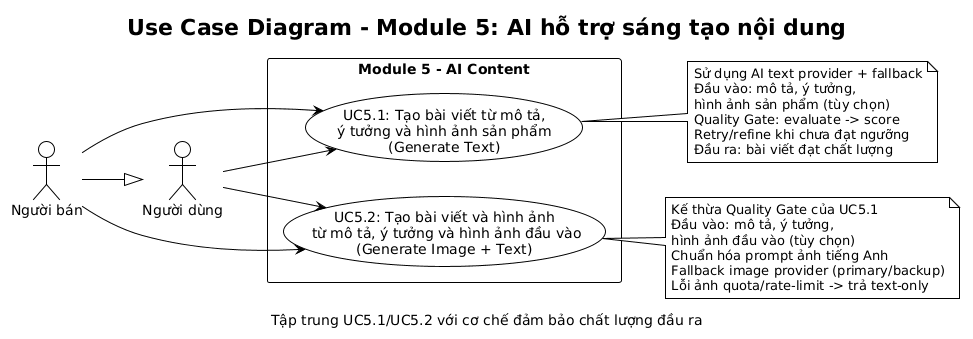
\includegraphics[width=\textwidth]{Images/Usecases/UC-M5-AI.png}
\caption{Sơ đồ Use Case cho Module 5: Tích hợp AI Hỗ trợ Sáng tạo}
\label{fig:usecase-module5}
\end{figure}

\renewcommand{\arraystretch}{1.3}

% UC5.1: GENERATE TEXT
\begin{longtable}{|p{3.5cm}|p{11cm}|}
\caption{Đặc tả Use Case AI Generate Text} \label{tab:uc5.1} \\
\hline
\endfirsthead

\multicolumn{2}{c}%
{{\bfseries \tablename\ \thetable{} -- tiếp tục từ trang trước}} \\
\hline
\endhead

\hline \multicolumn{2}{|r|}{{Tiếp tục ở trang sau}} \\ \hline
\endfoot

\hline
\endlastfoot

\textbf{Tên Use Case} & \textbf{UC5.1: Tạo bài viết từ mô tả, ý tưởng và hình ảnh sản phẩm (Generate Text)} \\ \hline
\textbf{Tác nhân} & Người dùng, Người bán \\ \hline
\textbf{Mô tả} & Cho phép người dùng tạo ra một bài viết hoàn chỉnh dựa trên mô tả, ý tưởng và hình ảnh sản phẩm (nếu có) sử dụng Google Gemini API, với quy trình đánh giá chất lượng tự động và cải thiện prompt khi kết quả chưa đạt. \\ \hline
\textbf{Kích hoạt} & Khi đang soạn thảo bài đăng, người dùng nhấn vào tùy chọn ``Tạo bài viết với AI''. \\ \hline
\textbf{Điều kiện tiên quyết} & 
\begin{itemize}
    \item Người dùng đã đăng nhập và đang trong giao diện tạo bài đăng.
    \item Người dùng đã nhập ít nhất một mô tả hoặc ý tưởng, có thể kèm theo hình ảnh sản phẩm.
\end{itemize} \\ \hline
\textbf{Điều kiện sau} & Một nội dung bài viết hoàn chỉnh (tiêu đề, nội dung, hashtags, CTA) được tạo ra và chèn vào trình soạn thảo, kèm theo điểm đánh giá chất lượng và gợi ý chỉnh sửa (nếu có). \\ \hline
\textbf{Luồng sự kiện chính} & 
\begin{enumerate}
    \item Người dùng nhập mô tả hoặc ý tưởng về bài viết (có thể tải lên hình ảnh sản phẩm).
    \item Người dùng nhấn nút ``Tạo bài viết với AI''.
    \item Hệ thống phân tích đầu vào: trích xuất thực thể chính (tên sản phẩm, đặc điểm, lợi ích), xác định giọng điệu và loại nội dung. Nếu có hình ảnh, phân tích nội dung hình ảnh bằng Gemini Vision.
    \item Hệ thống xây dựng prompt có cấu trúc gồm 5 phần: System Instruction (vai trò chuyên gia nội dung), Context (thông tin thương hiệu, nền tảng), User Input (mô tả + phân tích hình ảnh), Constraints (độ dài 100--300 từ, 5--10 hashtag, phải có CTA), Output Format (JSON schema).
    \item Hệ thống gửi prompt đến Google Gemini API và nhận kết quả.
    \item Hệ thống đánh giá chất lượng kết quả theo 6 tiêu chí có trọng số: Tính liên quan (0.25), Tính hấp dẫn (0.20), Cấu trúc hoàn chỉnh (0.15), Độ dài phù hợp (0.10), Chất lượng ngôn ngữ (0.15), Giá trị thương mại (0.15). Điểm tổng hợp là trung bình có trọng số.
    \item Nếu điểm $\geq$ 7.0/10: hệ thống hiển thị kết quả kèm điểm đánh giá. Nếu điểm $<$ 7.0 và chưa đạt giới hạn 3 lần thử: hệ thống xác định tiêu chí yếu nhất, bổ sung ràng buộc tương ứng vào prompt và gọi lại API (quay lại bước 5). Nếu đã hết lần thử: trả kết quả tốt nhất kèm gợi ý chỉnh sửa.
    \item Hệ thống hiển thị nội dung trong trình soạn thảo kèm điểm đánh giá chi tiết từng tiêu chí và gợi ý cải thiện.
\end{enumerate} \\ \hline
\textbf{Luồng thay thế} & 
\begin{itemize}
    \item A1: Người dùng không hài lòng với kết quả và nhấn ``Tạo lại'' để pipeline chạy lại từ đầu với prompt mới.
    \item A2: Người dùng chỉnh sửa trực tiếp nội dung trong editor (sửa tiêu đề, nội dung, thêm/bớt hashtag).
    \item A3: Người dùng chọn ``Viết lại đoạn này'' để AI viết lại chỉ đoạn được chọn với hướng dẫn cụ thể.
    \item A4: Người dùng thay đổi giọng điệu (chuyên nghiệp, thân thiện, hài hước, sang trọng) và yêu cầu AI viết lại theo giọng điệu mới.
\end{itemize} \\ \hline
\textbf{Ngoại lệ} & 
\begin{itemize}
    \item E1: Lỗi kết nối đến Gemini API $\rightarrow$ Hệ thống báo lỗi ``Không thể tạo nội dung lúc này, vui lòng thử lại sau''.
    \item E2: Hình ảnh không hợp lệ hoặc quá lớn $\rightarrow$ Hệ thống báo lỗi và yêu cầu tải lại hình ảnh.
    \item E3: Gemini API trả về nội dung vi phạm chính sách $\rightarrow$ Hệ thống lọc và yêu cầu tạo lại với prompt đã điều chỉnh.
\end{itemize} \\ \hline
\textbf{Ghi chú} & Pipeline sử dụng chính Gemini API để đánh giá chất lượng (meta-evaluation), kết hợp kiểm tra quy tắc tự động cho các tiêu chí có thể đo lường (format, length, hashtag count). Điểm đánh giá được hiển thị cho người dùng dưới dạng trực quan (thanh tiến trình hoặc biểu đồ radar). \\ \hline
\end{longtable}

% UC5.2: GENERATE IMAGE + TEXT
\begin{longtable}{|p{3.5cm}|p{11cm}|}
\caption{Đặc tả Use Case AI Generate Image + Text} \label{tab:uc5.2} \\
\hline
\endfirsthead

\multicolumn{2}{c}%
{{\bfseries \tablename\ \thetable{} -- tiếp tục từ trang trước}} \\
\hline
\endhead

\hline \multicolumn{2}{|r|}{{Tiếp tục ở trang sau}} \\ \hline
\endfoot

\hline
\endlastfoot

\textbf{Tên Use Case} & \textbf{UC5.2: Tạo bài viết và hình ảnh từ mô tả, ý tưởng và hình ảnh đầu vào (Generate Image + Text)} \\ \hline
\textbf{Tác nhân} & Người dùng, Người bán \\ \hline
\textbf{Mô tả} & Cho phép người dùng tự động tạo ra bài viết kèm hình ảnh dựa trên mô tả, ý tưởng và hình ảnh đầu vào (nếu có) sử dụng Google Gemini API, với đánh giá chất lượng riêng biệt cho text và image. \\ \hline
\textbf{Kích hoạt} & Khi đang soạn thảo bài đăng, người dùng nhấn vào tùy chọn ``Tạo bài viết và hình ảnh với AI''. \\ \hline
\textbf{Điều kiện tiên quyết} & 
\begin{itemize}
    \item Người dùng đã đăng nhập và đang trong giao diện tạo bài đăng.
    \item Người dùng đã nhập ít nhất một mô tả hoặc ý tưởng, có thể kèm theo hình ảnh đầu vào.
\end{itemize} \\ \hline
\textbf{Điều kiện sau} & Một bài viết hoàn chỉnh kèm hình ảnh được tạo bởi AI, cả hai đều được chèn vào trình soạn thảo kèm điểm đánh giá riêng biệt. \\ \hline
\textbf{Luồng sự kiện chính} & 
\begin{enumerate}
    \item Người dùng nhập mô tả hoặc ý tưởng (có thể tải lên hình ảnh đầu vào để tham khảo).
    \item Người dùng nhấn nút ``Tạo bài viết và hình ảnh với AI''.
    \item Hệ thống phân tích đầu vào (tương tự UC5.1), bổ sung phân tích phong cách hình ảnh (màu sắc chủ đạo, bố cục, đối tượng trong ảnh đầu vào).
    \item Hệ thống xây dựng prompt kép: prompt text (5 phần như UC5.1) và prompt image (System Instruction, Context từ text đã tạo, Visual Spec, Constraints về tỷ lệ 1:1/4:5, Negative Prompt).
    \item Hệ thống tạo text trước (với Evaluate--Refine Loop cho text), sau đó sử dụng text đã tạo làm context để tạo image (với Evaluate--Refine Loop riêng cho image).
    \item Đánh giá text: 6 tiêu chí (như UC5.1). Đánh giá image: 4 tiêu chí -- Tính liên quan (0.30), Chất lượng kỹ thuật (0.25), Tính thẩm mỹ (0.25), Nhất quán thương hiệu (0.20). Mỗi loại phải đạt $\geq$ 7.0/10.
    \item Nếu chỉ text hoặc chỉ image chưa đạt: hệ thống chỉ tạo lại phần chưa đạt, giữ nguyên phần đã tốt.
    \item Hệ thống hiển thị bài viết và hình ảnh kèm điểm đánh giá riêng cho từng loại.
\end{enumerate} \\ \hline
\textbf{Luồng thay thế} & 
\begin{itemize}
    \item A1: Người dùng nhấn ``Tạo lại'' để pipeline chạy lại từ đầu.
    \item A2: Người dùng chỉnh sửa text hoặc thay thế hình ảnh riêng biệt.
    \item A3: Người dùng chọn phong cách hình ảnh khác (photorealistic, illustration, flat design) và yêu cầu tạo lại chỉ hình ảnh.
    \item A4: Người dùng tải lên hình ảnh thay thế từ thiết bị, chỉ sử dụng text do AI tạo.
    \item A5: Người dùng yêu cầu AI chỉnh sửa hình ảnh cụ thể (thay đổi màu nền, thêm/bớt đối tượng).
\end{itemize} \\ \hline
\textbf{Ngoại lệ} & 
\begin{itemize}
    \item E1: Lỗi kết nối đến Gemini API $\rightarrow$ Hệ thống báo lỗi ``Không thể tạo nội dung lúc này, vui lòng thử lại sau''.
    \item E2: Gemini API không thể tạo hình ảnh phù hợp sau 3 lần thử $\rightarrow$ Hệ thống trả về bài viết kèm thông báo và gợi ý chỉnh sửa prompt hình ảnh.
    \item E3: Hình ảnh đầu vào không hợp lệ $\rightarrow$ Hệ thống báo lỗi và yêu cầu tải lại hình ảnh.
\end{itemize} \\ \hline
\textbf{Ghi chú} & Hai Evaluate--Refine Loop chạy tuần tự (text trước, image sau) để đảm bảo hình ảnh phù hợp với nội dung text. Chỉ phần chưa đạt ngưỡng mới được tạo lại, tối ưu chi phí gọi API. \\ \hline
\end{longtable}

% UC5.3: GENERATE VIDEO + IMAGES + TEXT
\begin{longtable}{|p{3.5cm}|p{11cm}|}
\caption{Đặc tả Use Case AI Generate Video + Images + Text} \label{tab:uc5.3} \\
\hline
\endfirsthead

\multicolumn{2}{c}%
{{\bfseries \tablename\ \thetable{} -- tiếp tục từ trang trước}} \\
\hline
\endhead

\hline \multicolumn{2}{|r|}{{Tiếp tục ở trang sau}} \\ \hline
\endfoot

\hline
\endlastfoot

\textbf{Tên Use Case} & \textbf{UC5.3: Tạo video ngắn, hình ảnh và bài viết từ mô tả, ý tưởng và hình ảnh đầu vào (Generate Video + Images + Text)} \\ \hline
\textbf{Tác nhân} & Người dùng, Người bán \\ \hline
\textbf{Mô tả} & Tính năng AI nâng cao nhất, tạo bài đăng đa phương thức (video ngắn + tối đa 3 hình ảnh + bài viết) với pipeline đánh giá ba tầng độc lập, sử dụng Google Gemini API và Google Veo 2. \\ \hline
\textbf{Kích hoạt} & Khi đang soạn thảo bài đăng, người dùng nhấn vào tùy chọn ``Tạo video và nội dung đa phương thức với AI''. \\ \hline
\textbf{Điều kiện tiên quyết} & 
\begin{itemize}
    \item Người dùng đã đăng nhập và đang trong giao diện tạo bài đăng.
    \item Người dùng đã nhập ít nhất một mô tả hoặc ý tưởng, có thể kèm theo hình ảnh đầu vào.
\end{itemize} \\ \hline
\textbf{Điều kiện sau} & Một bài đăng đa phương thức hoàn chỉnh (video + images + text) kèm điểm đánh giá từng loại được chèn vào trình soạn thảo. \\ \hline
\textbf{Luồng sự kiện chính} & 
\begin{enumerate}
    \item Người dùng nhập mô tả hoặc ý tưởng (có thể tải lên hình ảnh đầu vào).
    \item Người dùng nhấn nút ``Tạo video và nội dung đa phương thức với AI''.
    \item Hệ thống phân tích đầu vào (tương tự UC5.2), bổ sung xác định storyboard concept (cảnh mở đầu, giới thiệu, highlight, CTA).
    \item Hệ thống thực hiện pipeline tuần tự ba tầng:
    \begin{itemize}
        \item \textbf{Tầng 1 -- Text}: Xây dựng prompt text $\rightarrow$ Gemini API $\rightarrow$ Đánh giá 6 tiêu chí $\rightarrow$ Evaluate--Refine Loop (tối đa 3 lần).
        \item \textbf{Tầng 2 -- Images}: Dùng text làm context $\rightarrow$ Xây dựng prompt image $\rightarrow$ Gemini API tạo tối đa 3 ảnh $\rightarrow$ Đánh giá 4 tiêu chí mỗi ảnh $\rightarrow$ Evaluate--Refine Loop.
        \item \textbf{Tầng 3 -- Video}: Dùng text + images làm context $\rightarrow$ Tự động tạo storyboard $\rightarrow$ Xây dựng prompt video (15--30 giây, tỷ lệ 9:16/1:1) $\rightarrow$ Google Veo 2 $\rightarrow$ Đánh giá 5 tiêu chí: Tính mạch lạc (0.25), Chất lượng hình ảnh (0.25), Độ dài phù hợp (0.15), Tính hấp dẫn (0.20), Nhất quán nội dung (0.15) $\rightarrow$ Evaluate--Refine Loop.
    \end{itemize}
    \item Mỗi tầng Evaluate--Refine Loop chạy độc lập. Khi tạo lại tầng sau, kết quả tầng trước đã đạt được giữ nguyên.
    \item Hệ thống hiển thị video, hình ảnh và bài viết kèm điểm đánh giá chi tiết từng loại. Người dùng có thể chỉnh sửa hoặc tạo lại riêng từng thành phần.
\end{enumerate} \\ \hline
\textbf{Luồng thay thế} & 
\begin{itemize}
    \item A1: Người dùng nhấn ``Tạo lại'' toàn bộ để pipeline chạy lại từ đầu.
    \item A2: Người dùng tạo lại chỉ một thành phần (ví dụ: chỉ video) với yêu cầu bổ sung.
    \item A3: Người dùng chỉnh sửa text, thay thế hình ảnh hoặc video trước khi đăng.
    \item A4: Người dùng cung cấp storyboard chi tiết hơn để cải thiện chất lượng video.
    \item A5: Người dùng chỉ sử dụng một phần nội dung (ví dụ: text + images, bỏ video).
\end{itemize} \\ \hline
\textbf{Ngoại lệ} & 
\begin{itemize}
    \item E1: Lỗi kết nối đến Gemini API hoặc Google Veo 2 $\rightarrow$ Hệ thống báo lỗi.
    \item E2: Gemini API không thể tạo video phù hợp sau 3 lần thử $\rightarrow$ Hệ thống trả về images + text kèm gợi ý cải thiện prompt video.
    \item E3: Hình ảnh đầu vào không hợp lệ $\rightarrow$ Hệ thống báo lỗi.
    \item E4: Video vượt quá 30 giây $\rightarrow$ Kiểm tra rule-based đánh trượt, tự động tạo lại với ràng buộc thời lượng chặt hơn.
\end{itemize} \\ \hline
\textbf{Ghi chú} & Pipeline ba tầng đảm bảo tính nhất quán: text làm nền tảng cho images, text + images làm nền tảng cho video. Đánh giá ``Nhất quán nội dung'' (tiêu chí video) kiểm tra phong cách video có khớp với images và text đã tạo. \\ \hline
\end{longtable}

\subsection{Module 6: Lên lịch và Điều phối Bài đăng}
\subsubsection{Module 6: Lên lịch và Điều phối}
Module này cung cấp tiện ích giúp người dùng và người bán quản lý thời gian đăng bài hiệu quả, đảm bảo nội dung tiếp cận người xem vào khung giờ vàng.

\begin{figure}[H]
\centering
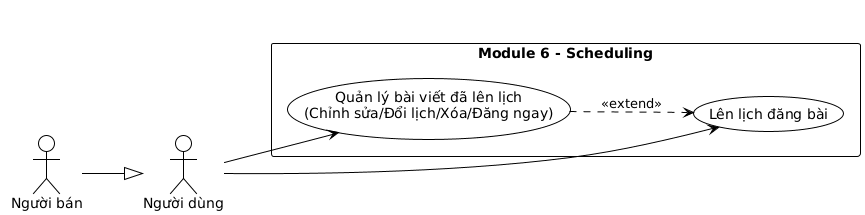
\includegraphics[width=\textwidth]{Images/Usecases/UC-M6-Scheduling.png}
\caption{Sơ đồ Use Case cho Module 6: Lên lịch và Điều phối Bài đăng}
\label{fig:usecase-module6}
\end{figure}

\renewcommand{\arraystretch}{1.3}

% UC6.1: LÊN LỊCH
\begin{table}[H]
\centering
\begin{tabularx}{\textwidth}{|l|X|}
\hline
\textbf{Tên Use Case} & \textbf{UC6.1: Lên lịch đăng bài} \\ \hline
\textbf{Tác nhân} & Người dùng, Người bán \\ \hline
\textbf{Mô tả} & Cung cấp cho người dùng tùy chọn để lên lịch cho một bài đăng, giúp bài viết được tự động xuất bản vào một thời điểm cụ thể trong tương lai. \\ \hline
\textbf{Kích hoạt} & Khi tạo một bài đăng mới, người dùng chọn tùy chọn ``Lên lịch'' thay vì ``Đăng ngay''. \\ \hline
\textbf{Điều kiện tiên quyết} & 
\begin{itemize}
    \item Người dùng đã đăng nhập vào hệ thống.
    \item Người dùng đang ở trong giao diện tạo bài đăng và đã có nội dung cho bài viết.
\end{itemize} \\ \hline
\textbf{Điều kiện sau} & 
\begin{itemize}
    \item Bài đăng được lưu vào cơ sở dữ liệu dưới dạng ``bản nháp đã lên lịch''.
    \item Bài đăng sẽ không hiển thị công khai cho đến đúng thời điểm đã được lên lịch.
\end{itemize} \\ \hline
\textbf{Luồng sự kiện chính} & 
\begin{enumerate}
    \item Trong giao diện tạo bài đăng, sau khi soạn xong nội dung, người dùng chọn tùy chọn ``Lên lịch''.
    \item Một giao diện chọn ngày và giờ trong tương lai sẽ hiện ra.
    \item Người dùng chọn ngày và giờ mong muốn để xuất bản bài viết.
    \item Người dùng nhấn nút ``Xác nhận Lịch''.
    \item Hệ thống lưu bài đăng với trạng thái ``đã lên lịch'' và thời điểm xuất bản đã chọn.
    \item Hệ thống hiển thị thông báo ``Bài viết đã được lên lịch thành công''.
\end{enumerate} \\ \hline
\textbf{Luồng thay thế} & 
\begin{itemize}
    \item A1: Người dùng quyết định không lên lịch nữa và chọn ``Đăng ngay''.
\end{itemize} \\ \hline
\textbf{Ngoại lệ} & 
\begin{itemize}
    \item E1: Người dùng chọn một thời điểm trong quá khứ $\rightarrow$ Hệ thống báo lỗi ``Vui lòng chọn một thời điểm trong tương lai''.
\end{itemize} \\ \hline
\textbf{Ghi chú} & Backend cần có một cơ chế (ví dụ: cron job) để kiểm tra và tự động xuất bản các bài đăng đã đến hạn. \\ \hline
\end{tabularx}
\caption{Đặc tả Use Case Lên lịch đăng bài}
\end{table}

% UC6.2: QUẢN LÝ LỊCH
\begin{table}[H]
\centering
\begin{tabularx}{\textwidth}{|l|X|}
\hline
\textbf{Tên Use Case} & \textbf{UC6.2: Quản lý bài viết đã lên lịch} \\ \hline
\textbf{Tác nhân} & Người dùng, Người bán \\ \hline
\textbf{Mô tả} & Cung cấp một giao diện để người dùng có thể xem lại danh sách các bài viết đang chờ xuất bản, cũng như chỉnh sửa, thay đổi lịch hoặc xóa chúng. \\ \hline
\textbf{Kích hoạt} & Người dùng truy cập vào một mục riêng trong trang cá nhân để xem các bài viết đã lên lịch. \\ \hline
\textbf{Điều kiện tiên quyết} & 
\begin{itemize}
    \item Người dùng đã đăng nhập vào hệ thống.
    \item Người dùng có ít nhất một bài viết đã được lên lịch.
\end{itemize} \\ \hline
\textbf{Điều kiện sau} & Bài viết đã lên lịch được cập nhật (thay đổi nội dung, thời gian) hoặc bị xóa khỏi hàng chờ xuất bản. \\ \hline
\textbf{Luồng sự kiện chính} & 
\begin{enumerate}
    \item Người dùng truy cập vào trang ``Quản lý bài viết đã lên lịch''.
    \item Hệ thống hiển thị danh sách các bài viết đang chờ, kèm theo nội dung xem trước và thời gian dự kiến đăng.
    \item Người dùng chọn một bài viết và thực hiện một trong các hành động: Chỉnh sửa nội dung; Thay đổi lịch; Xóa; Đăng ngay.
    \item Hệ thống cập nhật thay đổi tương ứng vào cơ sở dữ liệu.
\end{enumerate} \\ \hline
\textbf{Luồng thay thế} & 
\begin{itemize}
    \item A1: Người dùng chọn một bài viết và quyết định ``Đăng ngay'' thay vì chờ đến thời gian đã lên lịch.
\end{itemize} \\ \hline
\textbf{Ngoại lệ} & 
\begin{itemize}
    \item E1: Người dùng cố gắng chỉnh sửa một bài viết ngay tại thời điểm nó đang được hệ thống tự động xuất bản $\rightarrow$ Hệ thống báo lỗi hoặc thông báo bài viết đã được đăng.
\end{itemize} \\ \hline
\textbf{Ghi chú} & Giao diện này mang lại sự linh hoạt và quyền kiểm soát hoàn toàn cho người dùng đối với kế hoạch nội dung. \\ \hline
\end{tabularx}
\caption{Đặc tả Use Case Quản lý lịch đăng}
\end{table}

\subsection{Module 7: Hệ thống Thông báo}
\subsubsection{Module 7: Hệ thống Thông báo (Notification)}
Hệ thống thông báo thời gian thực (Real-time) đóng vai trò then chốt trong việc giữ chân người dùng và đảm bảo thông tin mua bán được cập nhật tức thì.

\begin{figure}[H]
\centering
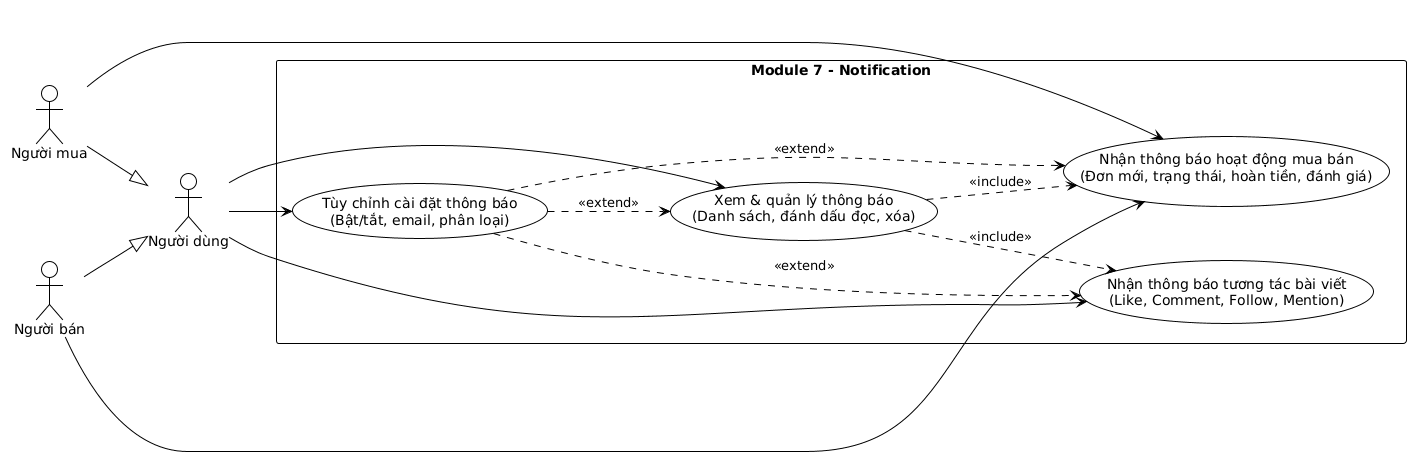
\includegraphics[width=\textwidth]{Images/Usecases/UC-M7-Notification.png}
\caption{Sơ đồ Use Case cho Module 7: Hệ thống Thông báo}
\label{fig:usecase-module7}
\end{figure}

\renewcommand{\arraystretch}{1.3}

% UC7.1: THÔNG BÁO TƯƠNG TÁC
\begin{table}[H]
\centering
\begin{tabularx}{\textwidth}{|l|X|}
\hline
\textbf{Tên Use Case} & \textbf{UC7.1: Nhận thông báo tương tác xã hội} \\ \hline
\textbf{Tác nhân} & Người dùng, Người bán \\ \hline
\textbf{Mô tả} & Hệ thống tự động gửi thông báo ngay lập tức đến người sở hữu bài viết khi có người khác thực hiện các hành động: thích bài viết, bình luận, theo dõi người dùng, hoặc được nhắc đến trong bình luận/bài viết của người khác. \\ \hline
\textbf{Kích hoạt} & Một người dùng khác thực hiện hành động tương tác với bài viết hoặc tài khoản của người nhận. \\ \hline
\textbf{Điều kiện tiên quyết} & 
\begin{itemize}
    \item Người nhận đã đăng nhập vào hệ thống ít nhất một lần trong phiên hiện tại.
    \item Người nhận không tắt hoàn toàn thông báo tương tác xã hội.
\end{itemize} \\ \hline
\textbf{Điều kiện sau} & 
\begin{itemize}
    \item Một thông báo mới xuất hiện trên giao diện người nhận.
    \item Số lượng thông báo chưa đọc tăng lên.
    \item Thông báo được lưu lại để người dùng có thể xem lại sau.
\end{itemize} \\ \hline
\textbf{Luồng sự kiện chính} & 
\begin{enumerate}
    \item Người dùng A thực hiện hành động (ví dụ: thích bài viết của Người dùng B).
    \item Hệ thống phát hiện hành động này.
    \item Hệ thống xác định chủ sở hữu bài viết (Người dùng B).
    \item Hệ thống tạo thông báo mới và gửi ngay lập tức đến Người dùng B.
    \item Giao diện của Người dùng B hiển thị thông báo.
    \item Người dùng B có thể nhấn vào thông báo để chuyển thẳng đến nội dung liên quan.
\end{enumerate} \\ \hline
\textbf{Luồng thay thế} & A1: Người dùng B đang không online $\rightarrow$ Thông báo vẫn được lưu và sẽ hiển thị ngay khi người đó đăng nhập lại. A2: Người dùng B tắt âm thanh thông báo $\rightarrow$ chỉ hiển thị hình ảnh. \\ \hline
\textbf{Ngoại lệ} & 
\begin{itemize}
    \item E1: Người dùng B đã chặn Người dùng A $\rightarrow$ Không gửi thông báo.
    \item E2: Bài viết ở chế độ riêng tư và Người dùng A không được phép xem $\rightarrow$ Không gửi thông báo.
\end{itemize} \\ \hline
\textbf{Ghi chú} & Tính năng quan trọng giúp tăng tính tương tác xã hội. \\ \hline
\end{tabularx}
\caption{Đặc tả Use Case Thông báo tương tác}
\end{table}

% UC7.2: THÔNG BÁO MUA BÁN
\begin{table}[H]
\centering
\begin{tabularx}{\textwidth}{|l|X|}
\hline
\textbf{Tên Use Case} & \textbf{UC7.2: Nhận thông báo hoạt động mua bán} \\ \hline
\textbf{Tác nhân} & Người mua, Người bán \\ \hline
\textbf{Mô tả} & Khi có sự kiện liên quan đến đơn hàng (đặt hàng mới, người bán xác nhận, giao hàng, hoàn thành, hủy đơn, yêu cầu hoàn tiền, có đánh giá mới…), hệ thống gửi thông báo ngay cho cả hai bên liên quan. \\ \hline
\textbf{Kích hoạt} & Bất kỳ thay đổi trạng thái nào của đơn hàng hoặc hành động liên quan đến đơn hàng. \\ \hline
\textbf{Điều kiện tiên quyết} & 
\begin{itemize}
    \item Người nhận có ít nhất một đơn hàng đang trong quá trình xử lý hoặc vừa hoàn tất.
    \item Người nhận chưa tắt thông báo liên quan đến mua bán.
\end{itemize} \\ \hline
\textbf{Điều kiện sau} & 
\begin{itemize}
    \item Cả người mua và người bán đều nhận được thông báo ngay lập tức.
    \item Thông báo chứa liên kết dẫn trực tiếp đến trang chi tiết đơn hàng.
\end{itemize} \\ \hline
\textbf{Luồng sự kiện chính} & 
\begin{enumerate}
    \item Người mua đặt một đơn hàng mới.
    \item Hệ thống tạo thông báo ``Bạn có đơn hàng mới'' gửi đến Người bán.
    \item Người bán xác nhận đơn hàng.
    \item Hệ thống gửi thông báo ``Đơn hàng của bạn đã được xác nhận'' cho Người mua.
    \item Tương tự với các trạng thái: đang giao, đã giao, hoàn thành, hủy, có đánh giá mới, có yêu cầu hoàn tiền…
\end{enumerate} \\ \hline
\textbf{Luồng thay thế} & A1: Một bên đang offline $\rightarrow$ Thông báo được lưu và hiển thị khi đăng nhập lại. A2: Có thể gửi thêm email nếu người dùng bật tùy chọn này. \\ \hline
\textbf{Ngoại lệ} & E1: Đơn hàng bị hủy ngay lập tức bởi người mua trước khi người bán nhìn thấy $\rightarrow$ chỉ gửi thông báo hủy. \\ \hline
\textbf{Ghi chú} & Tính năng này giúp người bán phản hồi nhanh đơn hàng và người mua luôn nắm được trạng thái mua sắm. \\ \hline
\end{tabularx}
\caption{Đặc tả Use Case Thông báo đơn hàng}
\end{table}

% UC7.3: QUẢN LÝ THÔNG BÁO
\begin{table}[H]
\centering
\begin{tabularx}{\textwidth}{|l|X|}
\hline
\textbf{Tên Use Case} & \textbf{UC7.3: Xem và quản lý danh sách thông báo} \\ \hline
\textbf{Tác nhân} & Người dùng \\ \hline
\textbf{Mô tả} & Người dùng có thể mở ra xem toàn bộ danh sách thông báo đã nhận (cả đã đọc và chưa đọc), đánh dấu đã đọc, hoặc xóa thông báo không còn cần thiết. \\ \hline
\textbf{Kích hoạt} & Người dùng nhấn vào biểu tượng chuông hoặc mục ``Thông báo'' trên thanh điều hướng. \\ \hline
\textbf{Điều kiện tiên quyết} & Người dùng đã đăng nhập và từng nhận ít nhất một thông báo. \\ \hline
\textbf{Điều kiện sau} & 
\begin{itemize}
    \item Danh sách thông báo được cập nhật trạng thái đọc/xóa theo hành động của người dùng.
    \item Số lượng thông báo chưa đọc giảm tương ứng.
\end{itemize} \\ \hline
\textbf{Luồng sự kiện chính} & 
\begin{enumerate}
    \item Người dùng nhấn vào biểu tượng thông báo.
    \item Hệ thống hiển thị danh sách tất cả thông báo (mới nhất ở trên).
    \item Thông báo chưa đọc được làm nổi bật.
    \item Người dùng có thể: Nhấn vào thông báo; Đánh dấu đã đọc; Xóa.
    \item Hệ thống cập nhật lại trạng thái và giao diện ngay lập tức.
\end{enumerate} \\ \hline
\textbf{Luồng thay thế} & A1: Người dùng chọn ``Xóa tất cả thông báo'' $\rightarrow$ toàn bộ thông báo bị xóa vĩnh viễn. \\ \hline
\textbf{Ngoại lệ} & E1: Không có thông báo nào $\rightarrow$ hiển thị dòng chữ ``Bạn chưa có thông báo nào''. \\ \hline
\textbf{Ghi chú} & Giao diện nên hỗ trợ phân loại thông báo để dễ theo dõi. \\ \hline
\end{tabularx}
\caption{Đặc tả Use Case Quản lý danh sách thông báo}
\end{table}

% UC7.4: CÀI ĐẶT THÔNG BÁO
\begin{table}[H]
\centering
\begin{tabularx}{\textwidth}{|l|X|}
\hline
\textbf{Tên Use Case} & \textbf{UC7.4: Tùy chỉnh cài đặt thông báo} \\ \hline
\textbf{Tác nhân} & Người dùng \\ \hline
\textbf{Mô tả} & Người dùng có thể tự quyết định sẽ nhận loại thông báo nào, qua kênh nào (trên web, âm thanh, email), và tắt hoàn toàn một số loại thông báo nếu muốn. \\ \hline
\textbf{Kích hoạt} & Người dùng vào phần Cài đặt $\rightarrow$ Thông báo. \\ \hline
\textbf{Điều kiện tiên quyết} & Người dùng đã đăng nhập. \\ \hline
\textbf{Điều kiện sau} & Cài đặt thông báo của người dùng được lưu lại và áp dụng cho mọi phiên đăng nhập sau này. \\ \hline
\textbf{Luồng sự kiện chính} & 
\begin{enumerate}
    \item Người dùng vào Trang cá nhân $\rightarrow$ Cài đặt $\rightarrow$ Thông báo.
    \item Hệ thống hiển thị danh sách các loại thông báo có thể bật/tắt.
    \item Người dùng bật/tắt từng mục và chọn có nhận qua email hay không.
    \item Người dùng nhấn ``Lưu cài đặt''.
    \item Hệ thống lưu và áp dụng ngay lập tức.
\end{enumerate} \\ \hline
\textbf{Luồng thay thế} & A1: Người dùng chọn ``Tắt tất cả thông báo'' $\rightarrow$ toàn bộ thông báo (trừ thông báo hệ thống bắt buộc) sẽ không hiển thị nữa. \\ \hline
\textbf{Ngoại lệ} & Không có. \\ \hline
\textbf{Ghi chú} & Tính năng này quan trọng để tránh làm phiền và tăng trải nghiệm cá nhân hóa. \\ \hline
\end{tabularx}
\caption{Đặc tả Use Case Cài đặt thông báo}
\end{table}

\section{Activity diagram}
Phần này trình bày các Activity Diagrams mô tả dòng chảy nghiệp vụ, điểm quyết định, trạng thái và phản hồi của hệ thống theo từng module. Mỗi module có mô tả tổng quan và các diagram chi tiết với hình ảnh minh họa.

\subsection{Module 1 – Authentication \& Profile}

Module này bao quát hành trình xác thực người dùng: đăng ký, đăng nhập với 2FA, khôi phục mật khẩu, quản lý hồ sơ, cài đặt quyền riêng tư và nâng cấp lên Seller.

\subsubsection{AD-M1-Auth-Register-Login}

Diagram này mô tả quy trình đăng ký và đăng nhập của người dùng, bao gồm ba use case chính.

\textbf{UC1.1 – Đăng ký tài khoản:} Người dùng nhập email, mật khẩu và thông tin cá nhân. Hệ thống kiểm tra tính hợp lệ và email đã tồn tại chưa. Nếu hợp lệ, hệ thống tạo tài khoản với trạng thái \textit{unverified} và gửi email xác thực. Sau khi người dùng xác thực, hệ thống kích hoạt tài khoản.

\textbf{UC1.2 – Đăng nhập:} Người dùng nhập email và mật khẩu. Hệ thống xác thực thông tin. Nếu đúng và không bật 2FA, hệ thống tạo JWT và chuyển hướng đến Trang chủ. Nếu bật 2FA, quy trình chuyển sang UC1.3.

\textbf{UC1.3 – Xác thực hai yếu tố (2FA):} Sau khi xác thực email/mật khẩu, hệ thống gửi mã OTP. Người dùng nhập mã OTP. Nếu mã hợp lệ và chưa hết hạn, hệ thống tạo JWT và chuyển hướng đến Trang chủ.

\begin{figure}[H]
  \centering
  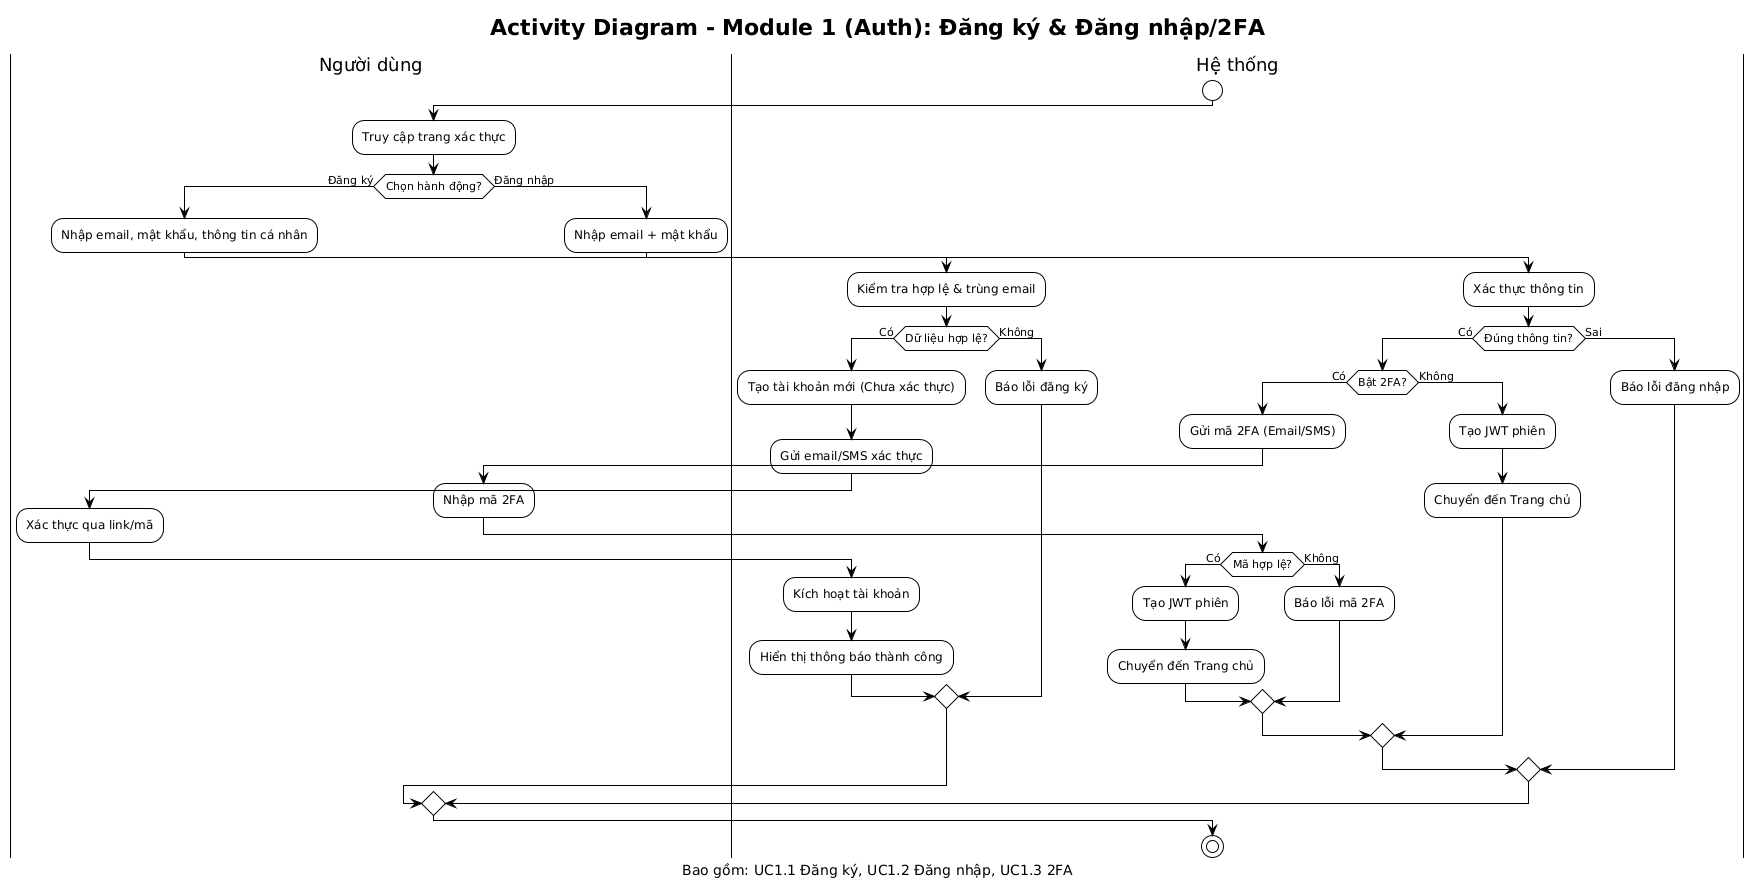
\includegraphics[width=\textwidth]{Images/Activity diagrams/AD-M1-Auth-Register-Login.png}
  \caption{Activity Diagram - Đăng ký và Đăng nhập (AD-M1-Auth-Register-Login)}
\end{figure}

\subsubsection{AD-M1-Auth-Recovery-Logout}

Diagram này mô tả quy trình khôi phục mật khẩu và đăng xuất của người dùng.

\textbf{UC1.4 – Khôi phục mật khẩu:} Người dùng nhập email. Hệ thống kiểm tra và gửi link/mã OTP (bảo mật: luôn trả về thông báo chung). Người dùng mở link/nhập mã và đặt mật khẩu mới. Hệ thống xác thực và cập nhật mật khẩu.

\textbf{UC1.5 – Đăng xuất:} Người dùng nhấn "Đăng xuất". Hệ thống hủy phiên, xóa JWT token và blacklist token trên server, sau đó chuyển hướng về Trang chủ.

\begin{figure}[H]
  \centering
  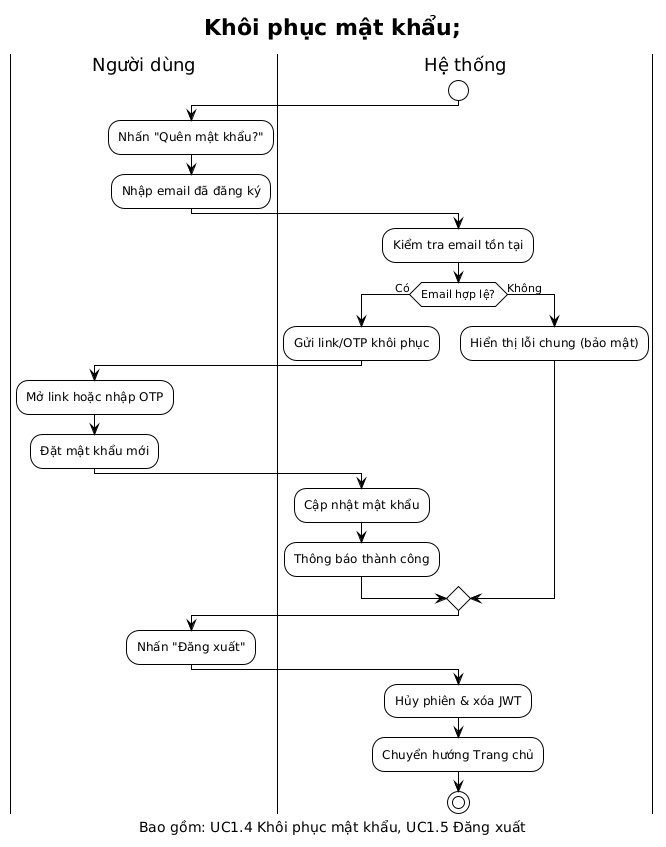
\includegraphics[width=\textwidth]{Images/Activity diagrams/AD-M1-Auth-Recovery-Logout.png}
  \caption{Activity Diagram - Khôi phục mật khẩu và Đăng xuất (AD-M1-Auth-Recovery-Logout)}
\end{figure}

\subsubsection{AD-M1-Profile-EditPrivacy}

Diagram này mô tả quy trình chỉnh sửa hồ sơ cá nhân và cài đặt quyền riêng tư.

\textbf{UC1.6 – Quản lý hồ sơ:} Người dùng cập nhật thông tin (bio, ảnh đại diện, ảnh bìa). Hệ thống upload ảnh (nếu có), xác thực dữ liệu, và cập nhật thông tin trong database. Nếu có lỗi, hệ thống trả về thông báo lỗi cụ thể.

\textbf{UC1.7 – Quyền riêng tư:} Người dùng điều chỉnh cài đặt ai có thể xem hồ sơ, bài đăng và nhắn tin (công khai, chỉ bạn bè, chỉ mình tôi). Hệ thống lưu cấu hình vào database và áp dụng ngay lập tức.

\begin{figure}[H]
  \centering
  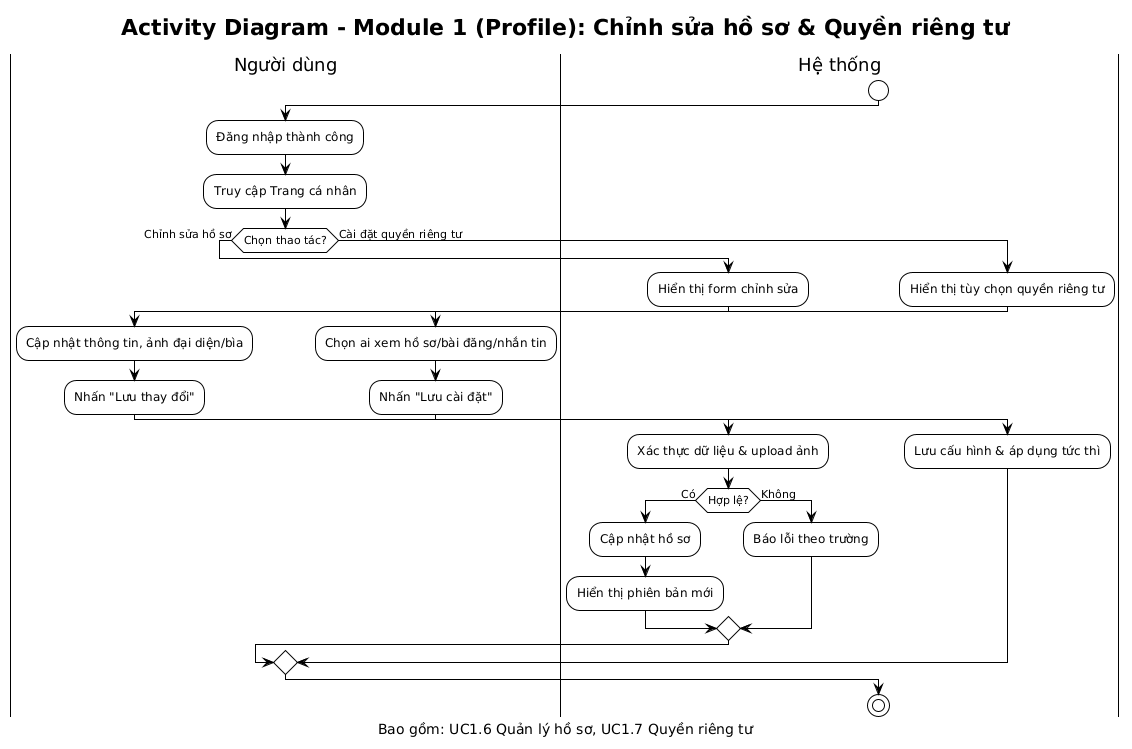
\includegraphics[width=\textwidth]{Images/Activity diagrams/AD-M1-Profile-EditPrivacy.png}
  \caption{Activity Diagram - Chỉnh sửa hồ sơ và Quyền riêng tư (AD-M1-Profile-EditPrivacy)}
\end{figure}

\subsubsection{AD-M1-Profile-SellerUpgrade}

Diagram này mô tả quy trình đăng ký trở thành người bán (Seller).

\textbf{UC1.8 – Đăng ký Người bán:} Buyer điền form đăng ký với thông tin shop (tên shop, địa chỉ, số điện thoại, giấy tờ pháp lý). Hệ thống lưu với trạng thái \textit{pending} và gửi email xác minh. Sau khi xác minh thành công, hệ thống cập nhật trạng thái thành \textit{approved}, thay đổi vai trò từ \textit{buyer} sang \textit{seller}, và chuyển hướng đến Seller Dashboard.

\begin{figure}[H]
  \centering
  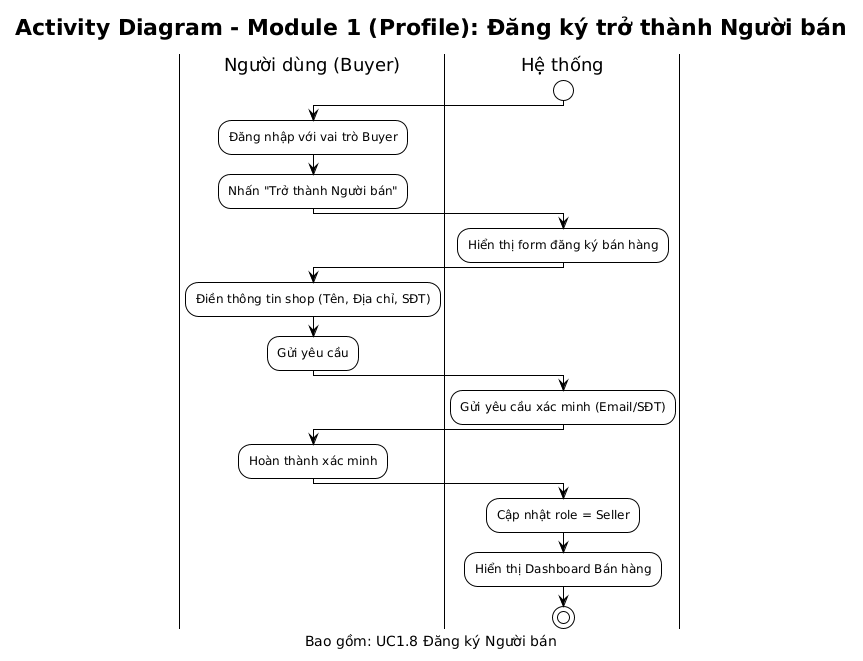
\includegraphics[width=\textwidth]{Images/Activity diagrams/AD-M1-Profile-SellerUpgrade.png}
  \caption{Activity Diagram - Đăng ký trở thành Người bán (AD-M1-Profile-SellerUpgrade)}
\end{figure}

\subsection{Module 2 – Social \& Content}

Module này tập trung vào các tính năng mạng xã hội: xem feed cá nhân hóa, tạo và quản lý bài đăng, tương tác, follow, nhắn tin, tham gia nhóm, và báo cáo vi phạm.

\subsubsection{AD-M2-FeedAndPosts}

Diagram này mô tả quy trình xem feed, tạo bài đăng và tương tác với nội dung.

\textbf{UC2.1 – Xem Feed:} Người dùng truy cập Trang chủ. Hệ thống truy vấn database lấy bài đăng từ người đang theo dõi kết hợp gợi ý, áp dụng thuật toán sắp xếp. Feed hiển thị với tính năng infinite scroll.

\textbf{UC2.2 – Tạo bài đăng:} Người dùng nhập nội dung văn bản và tải hình ảnh (nếu có). Seller có thể gắn thẻ sản phẩm (UC2.3). Hệ thống kiểm tra nội dung, lưu bài đăng vào database, và hiển thị trên feed.

\textbf{UC2.3 – Gắn thẻ sản phẩm:} Seller chọn một hoặc nhiều sản phẩm từ shop để gắn thẻ vào bài đăng. Người dùng xem bài đăng có thể nhấn vào thẻ sản phẩm để chuyển đến trang chi tiết.

\textbf{UC2.4 – Tương tác với bài đăng:} Người dùng có thể thích hoặc bình luận bài đăng. Hệ thống cập nhật số lượt thích/bình luận, lưu vào database và gửi thông báo đến chủ sở hữu bài đăng (UC7.1).

\begin{figure}[H]
  \centering
  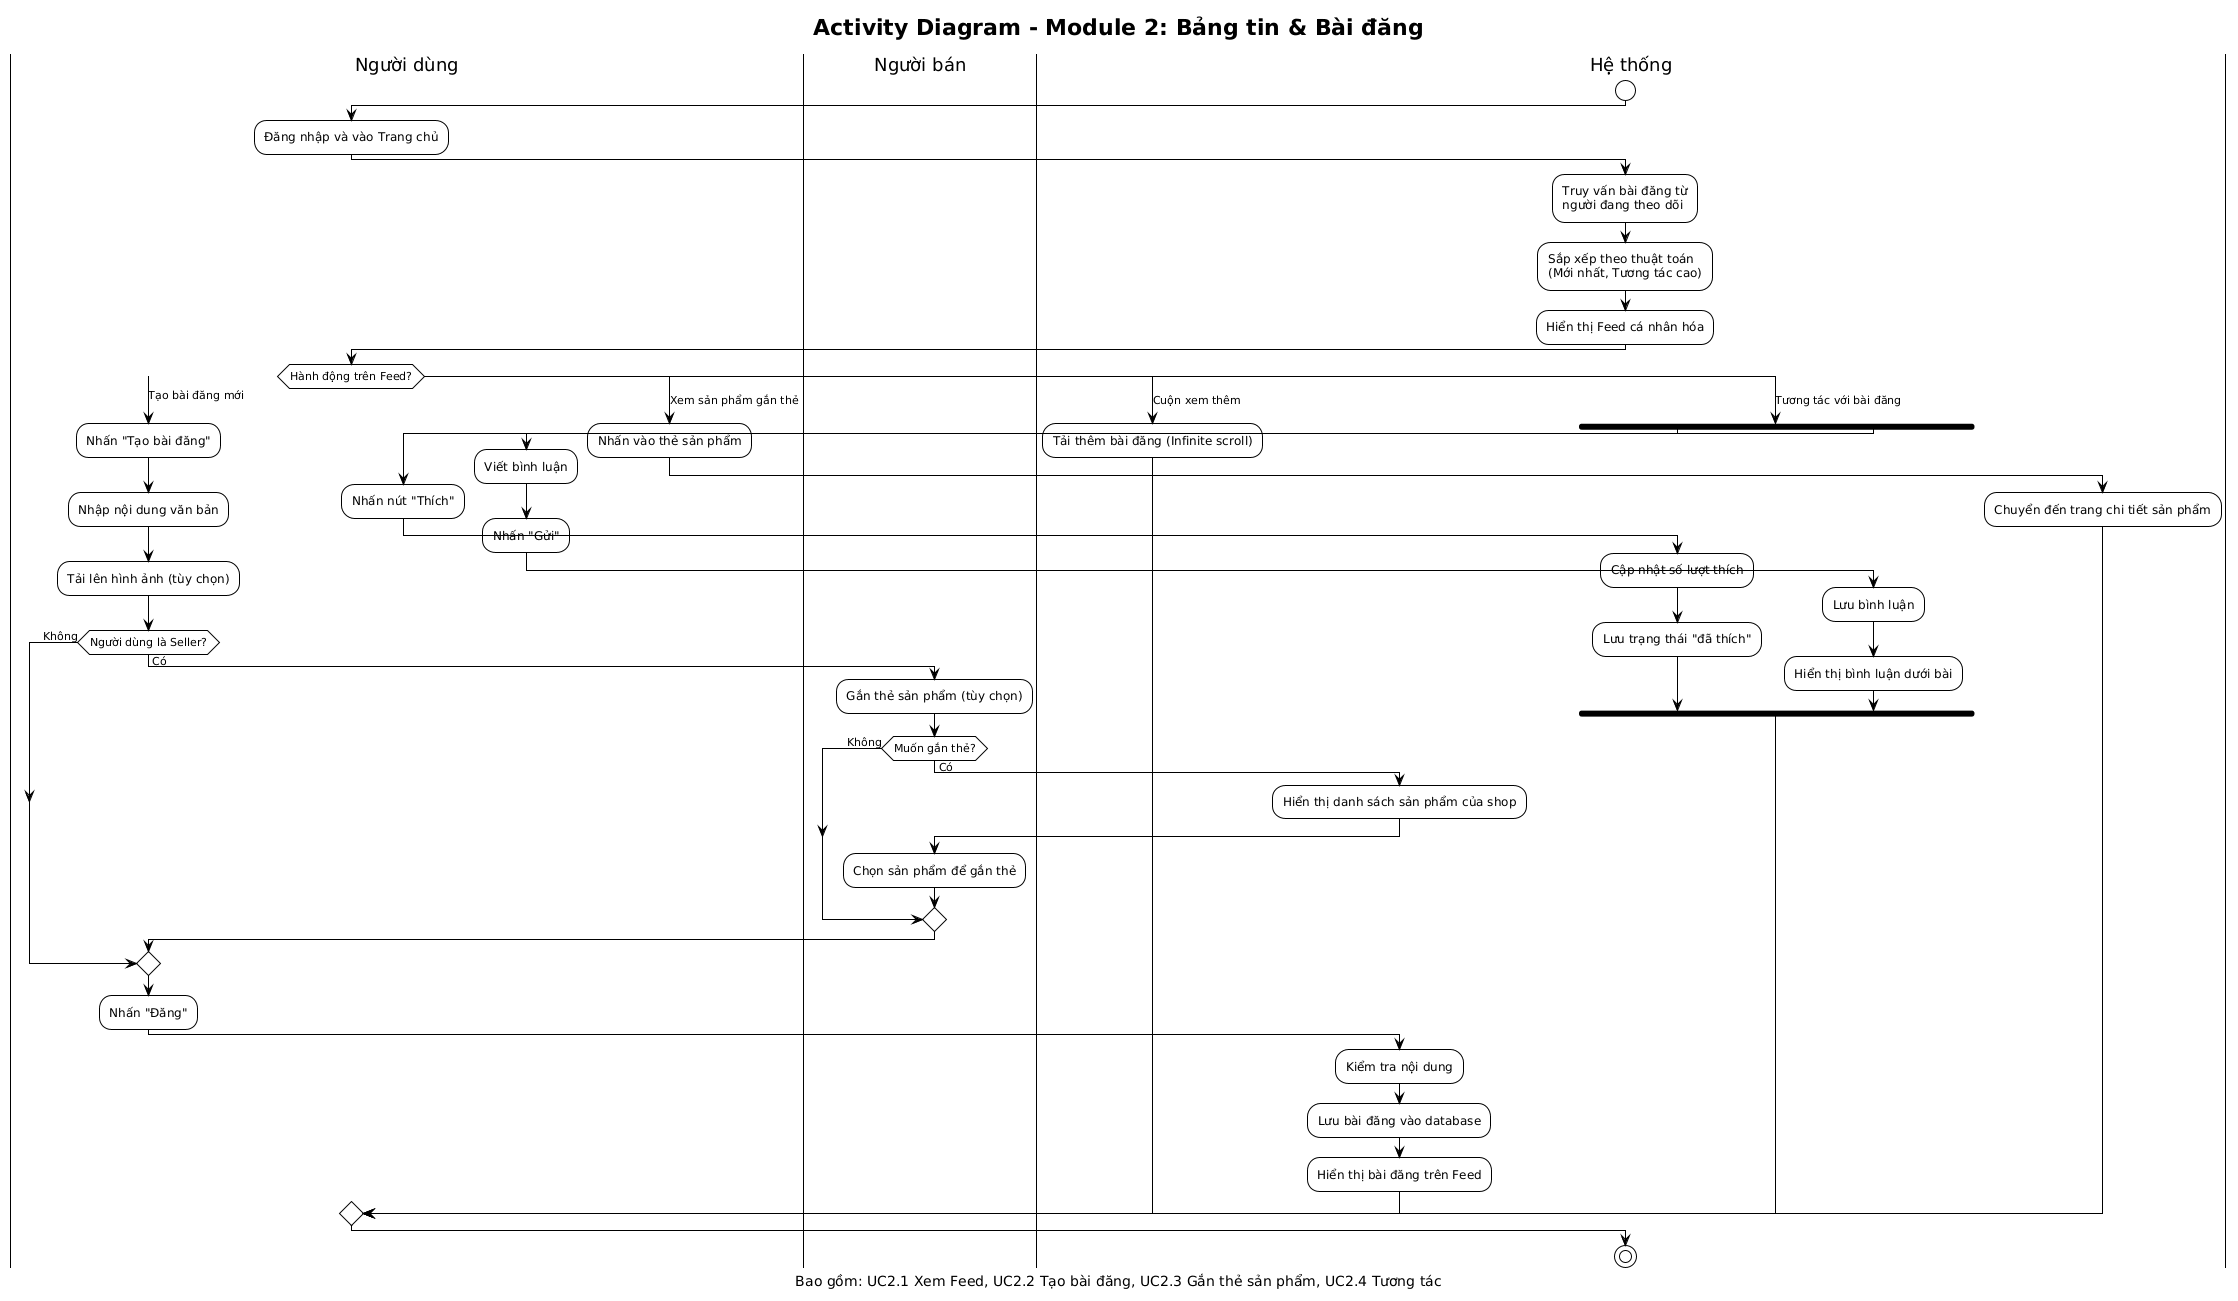
\includegraphics[width=\textwidth]{Images/Activity diagrams/AD-M2-FeedAndPosts.png}
  \caption{Activity Diagram - Feed và Bài đăng (AD-M2-FeedAndPosts)}
\end{figure}

\subsubsection{AD-M2-SocialConnections}

Diagram này mô tả các kết nối xã hội giữa người dùng, bao gồm follow, nhắn tin, tham gia nhóm và báo cáo vi phạm.

\textbf{UC2.5 – Theo dõi người dùng:} Người dùng A nhấn "Theo dõi" trên trang cá nhân của B. Hệ thống tạo mối quan hệ follow, cập nhật số người theo dõi, gửi thông báo đến B, và bài đăng của B sẽ xuất hiện trên Feed của A.

\textbf{UC2.6 – Nhắn tin 1-1:} Người dùng A gửi tin nhắn cho B. Hệ thống kiểm tra B có chặn A hay không. Nếu không bị chặn, hệ thống lưu tin nhắn vào database và gửi real-time đến B qua WebSocket (Socket.io).

\textbf{UC2.7 – Tham gia nhóm:} Người dùng A chọn nhóm và nhấn "Tham gia". Nếu là nhóm công khai, hệ thống thêm A vào nhóm ngay lập tức. Nếu là nhóm riêng tư, hệ thống gửi yêu cầu và chờ Admin phê duyệt.

\textbf{UC2.8 – Báo cáo vi phạm:} Người dùng A chọn đối tượng báo cáo (bài đăng, bình luận hoặc người dùng), chọn lý do vi phạm và thêm mô tả (nếu có). Hệ thống lưu báo cáo với trạng thái \textit{pending}, thông báo Admin và hiển thị "Báo cáo đã được ghi nhận".

\begin{figure}[H]
  \centering
  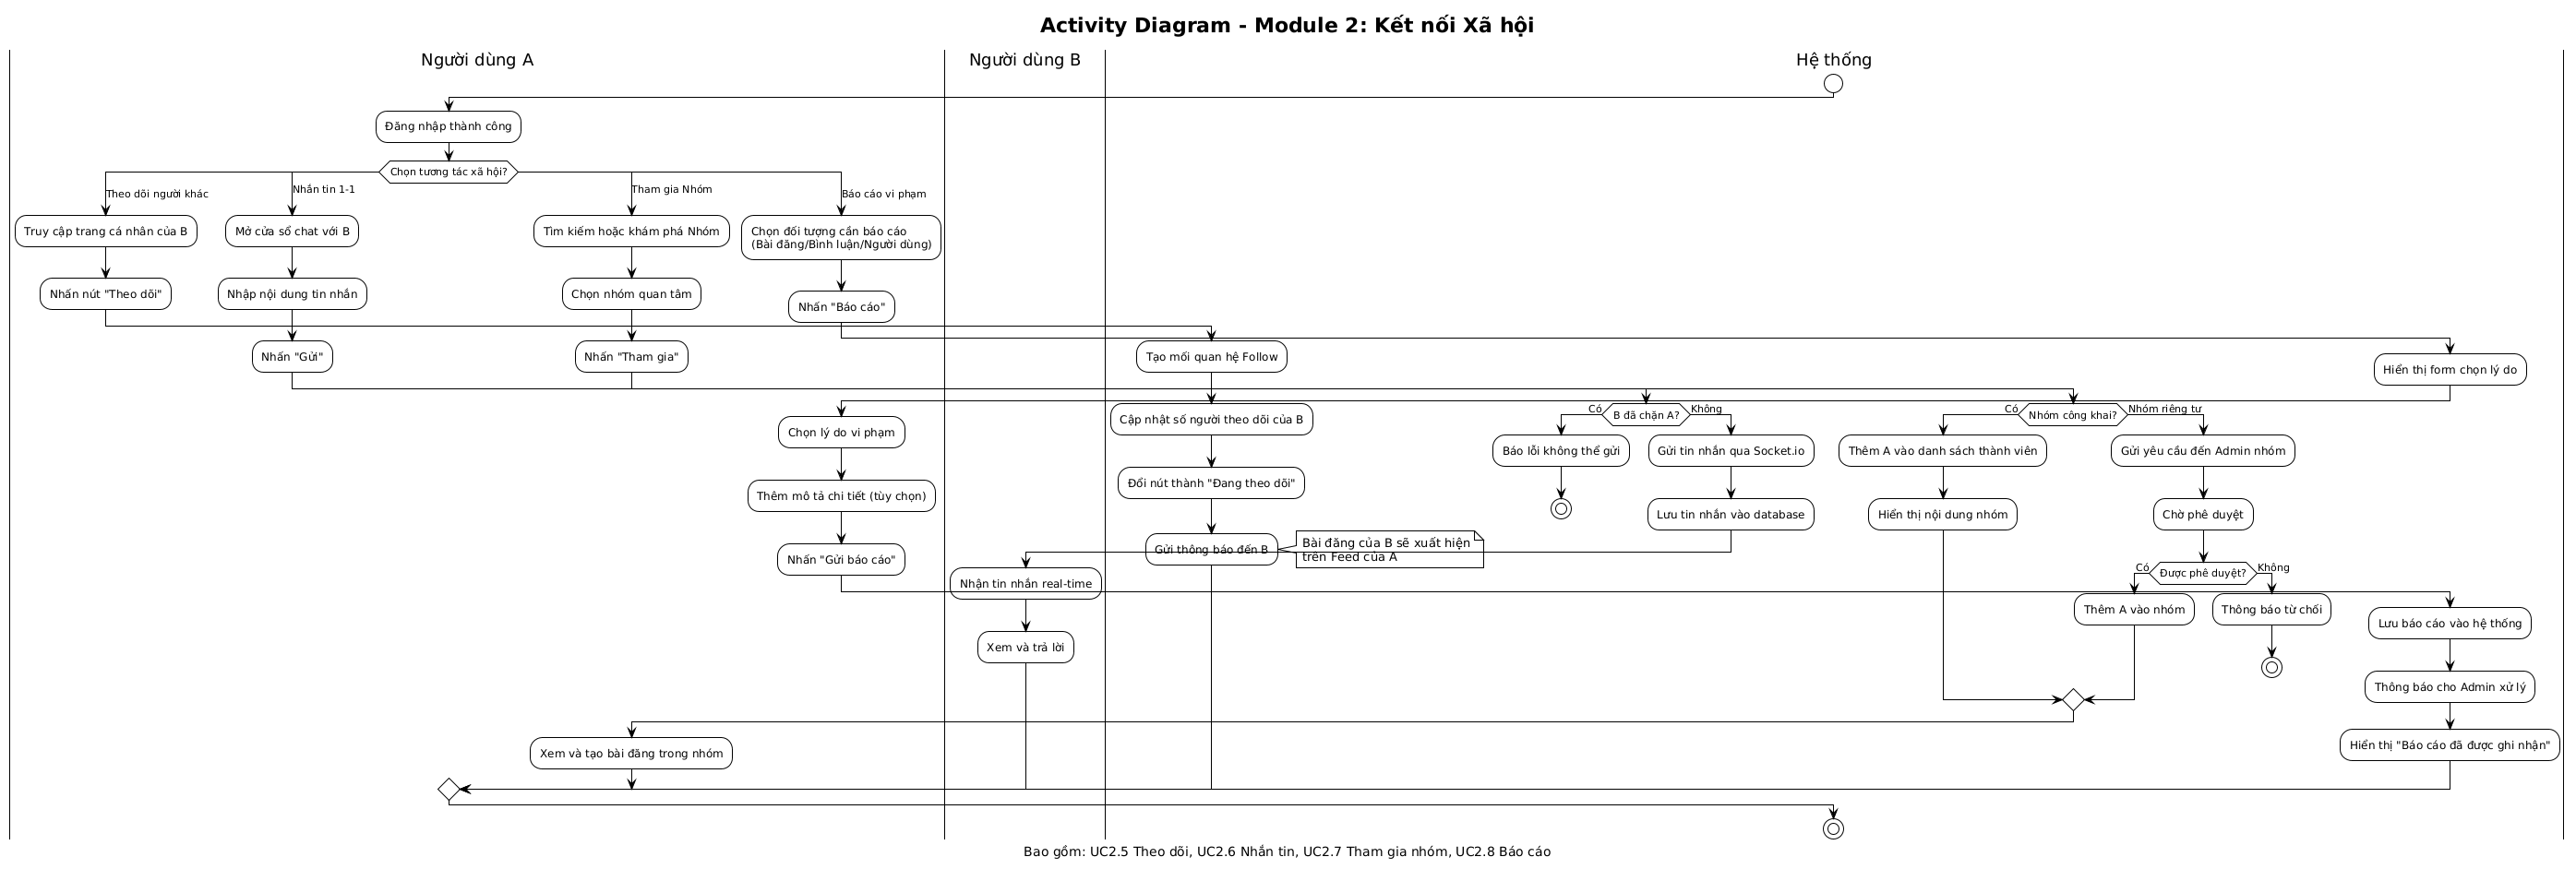
\includegraphics[width=\textwidth]{Images/Activity diagrams/AD-M2-SocialConnections.png}
  \caption{Activity Diagram - Kết nối Xã hội (AD-M2-SocialConnections)}
\end{figure}

\subsection{Module 3 – Commerce}

Module này bao quát hệ sinh thái thương mại điện tử: hành trình mua hàng của Buyer (tìm kiếm, xem sản phẩm, giỏ hàng, thanh toán, theo dõi đơn hàng, đánh giá) và quản lý của Seller (sản phẩm, đơn hàng, hoàn tiền, phản hồi đánh giá).

\subsubsection{AD-M3-BuyerFlow}

Diagram này mô tả toàn bộ quy trình mua hàng từ góc nhìn của người mua (Buyer).

\textbf{UC3.1 – Tìm kiếm và lọc sản phẩm:} Buyer nhập từ khóa và áp dụng bộ lọc (danh mục, khoảng giá, tags). Hệ thống truy vấn database và hiển thị danh sách sản phẩm phù hợp hoặc thông báo không tìm thấy.

\textbf{UC3.2 – Xem chi tiết sản phẩm và chọn biến thể:} Buyer chọn sản phẩm, hệ thống hiển thị chi tiết (hình ảnh, mô tả, giá, tồn kho, đánh giá). Buyer chọn biến thể (size, màu) và số lượng.

\textbf{UC3.3 – Thêm vào giỏ hàng:} Buyer nhấn "Thêm vào giỏ hàng". Hệ thống kiểm tra tồn kho, nếu còn hàng thì lưu vào giỏ hàng và cập nhật số lượng. Nếu hết hàng, hệ thống trả về lỗi và đề xuất sản phẩm tương tự.

\textbf{UC3.4 – Quản lý giỏ hàng:} Buyer truy cập giỏ hàng, hệ thống hiển thị danh sách sản phẩm và tổng tiền. Buyer có thể cập nhật số lượng hoặc xóa sản phẩm, hệ thống tự động tính lại tổng tiền.

\textbf{UC3.5 – Thanh toán:} Buyer nhấn "Thanh toán". Hệ thống kiểm tra tồn kho lần cuối. Nếu đủ hàng, Buyer nhập địa chỉ giao hàng và chọn phương thức thanh toán. Hệ thống tạo đơn hàng với trạng thái \textit{Processing}, làm rỗng giỏ hàng, gửi thông báo cho Seller và hiển thị "Đặt hàng thành công".

\textbf{UC3.6 – Theo dõi đơn hàng:} Buyer xem "Đơn hàng của tôi", hệ thống hiển thị danh sách đơn hàng với mã, trạng thái và ngày đặt. Buyer có thể xem chi tiết và theo dõi trạng thái real-time.

\textbf{UC3.7 – Đánh giá sản phẩm:} Khi đơn hàng đã giao (\textit{Delivered}), Buyer có thể đánh giá sản phẩm (chọn số sao, viết nhận xét, tải ảnh). Hệ thống lưu đánh giá và hiển thị trên trang chi tiết sản phẩm.

\begin{figure}[H]
  \centering
  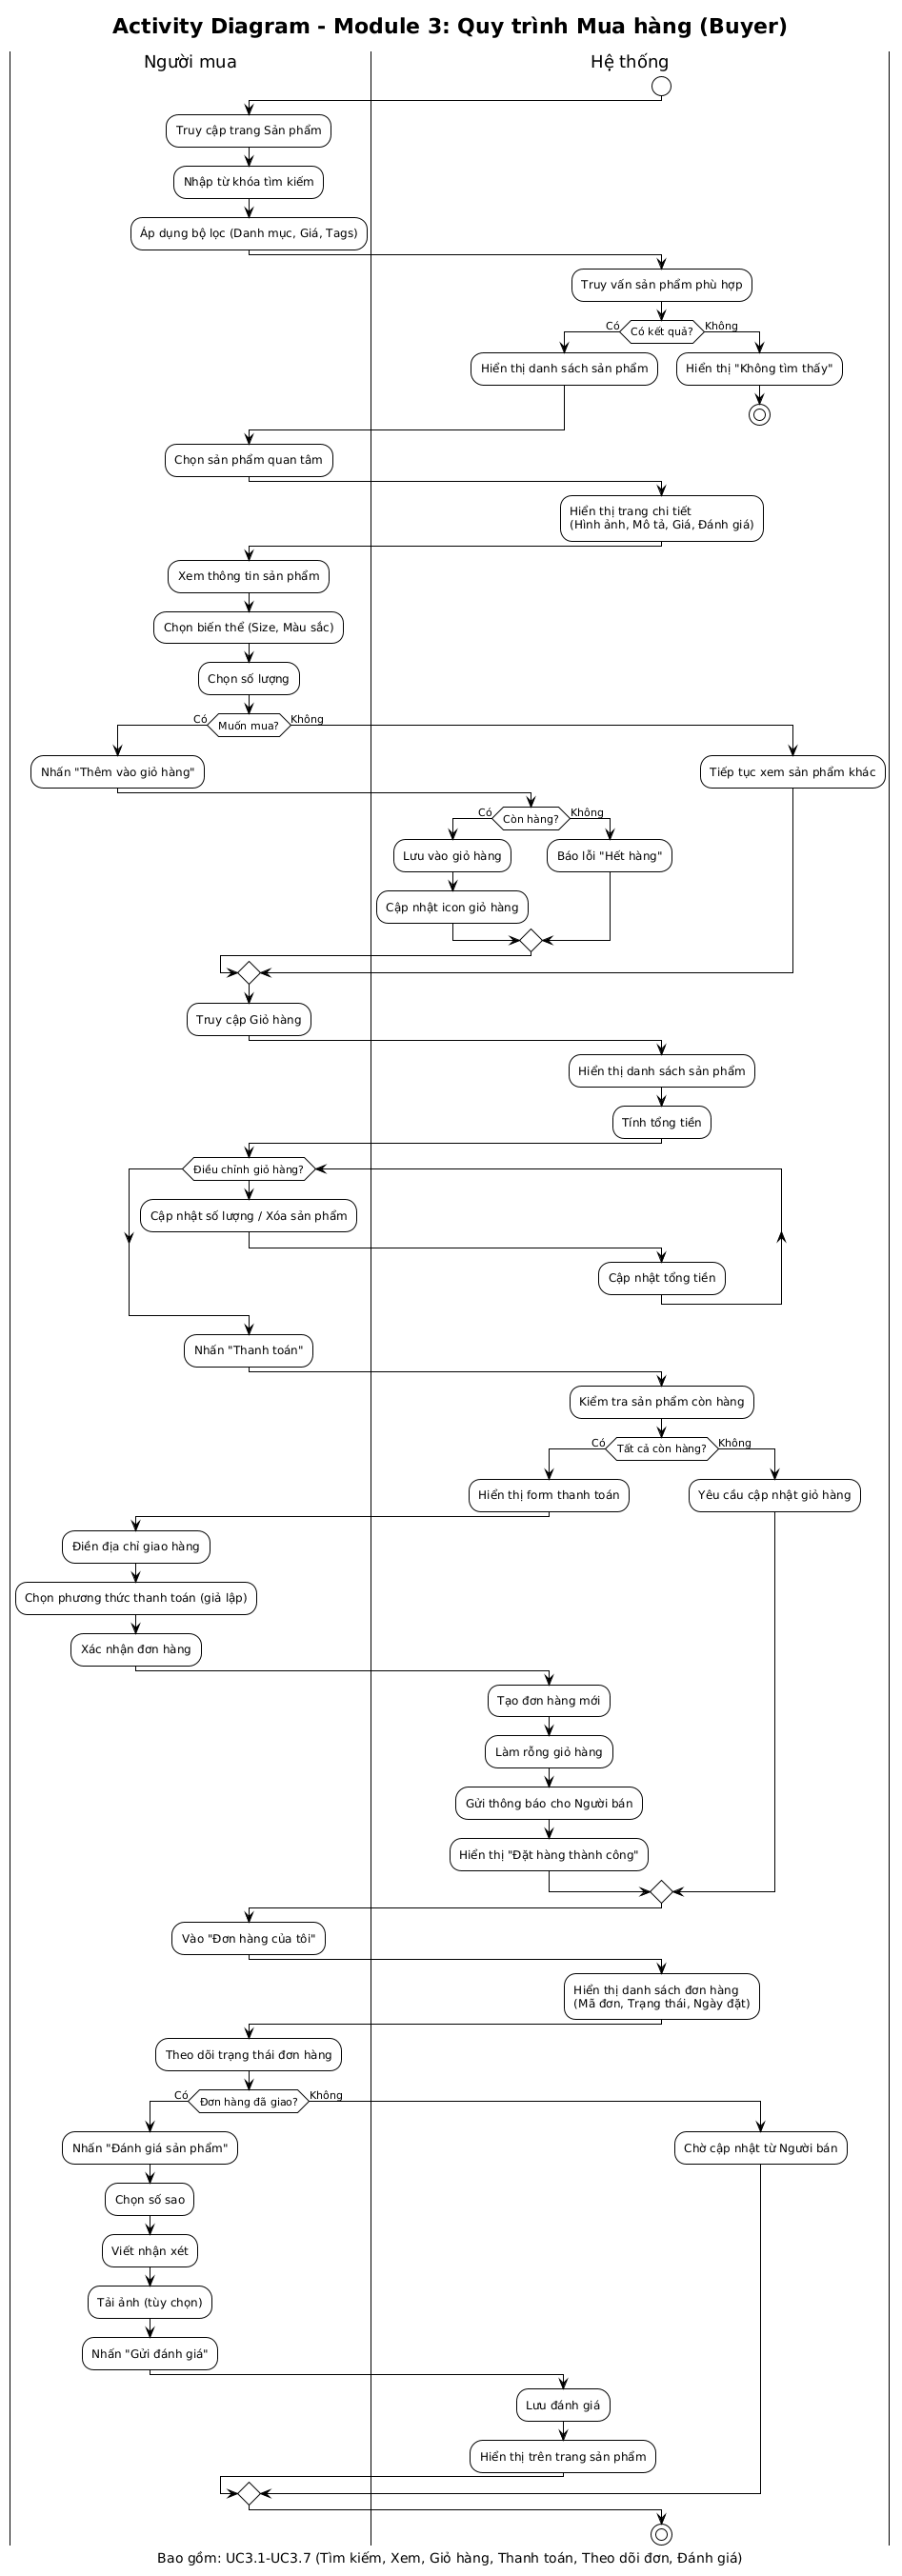
\includegraphics[width=\textwidth]{Images/Activity diagrams/AD-M3-BuyerFlow.png}
  \caption{Activity Diagram - Quy trình Mua hàng (AD-M3-BuyerFlow)}
\end{figure}

\subsubsection{AD-M3-Seller-ProductsOrders}

Diagram này mô tả các tác vụ quản lý sản phẩm và đơn hàng của Seller.

\textbf{UC3.8 – Quản lý sản phẩm:} Seller truy cập Dashboard Bán hàng, chọn "Quản lý Sản phẩm". Seller có thể thêm (tên, mô tả, giá, tồn kho, hình ảnh, biến thể), sửa hoặc xóa sản phẩm (soft delete). Hệ thống xác thực và lưu vào database.

\textbf{UC3.10 – Quản lý đơn hàng:} Seller chọn "Quản lý Đơn hàng", hệ thống hiển thị danh sách đơn hàng. Seller xem chi tiết và cập nhật trạng thái: "Đang xử lý", "Đang giao", "Đã giao", hoặc "Đã hủy". Hệ thống lưu thay đổi, ghi lịch sử và gửi thông báo đến Buyer.

\begin{figure}[H]
  \centering
  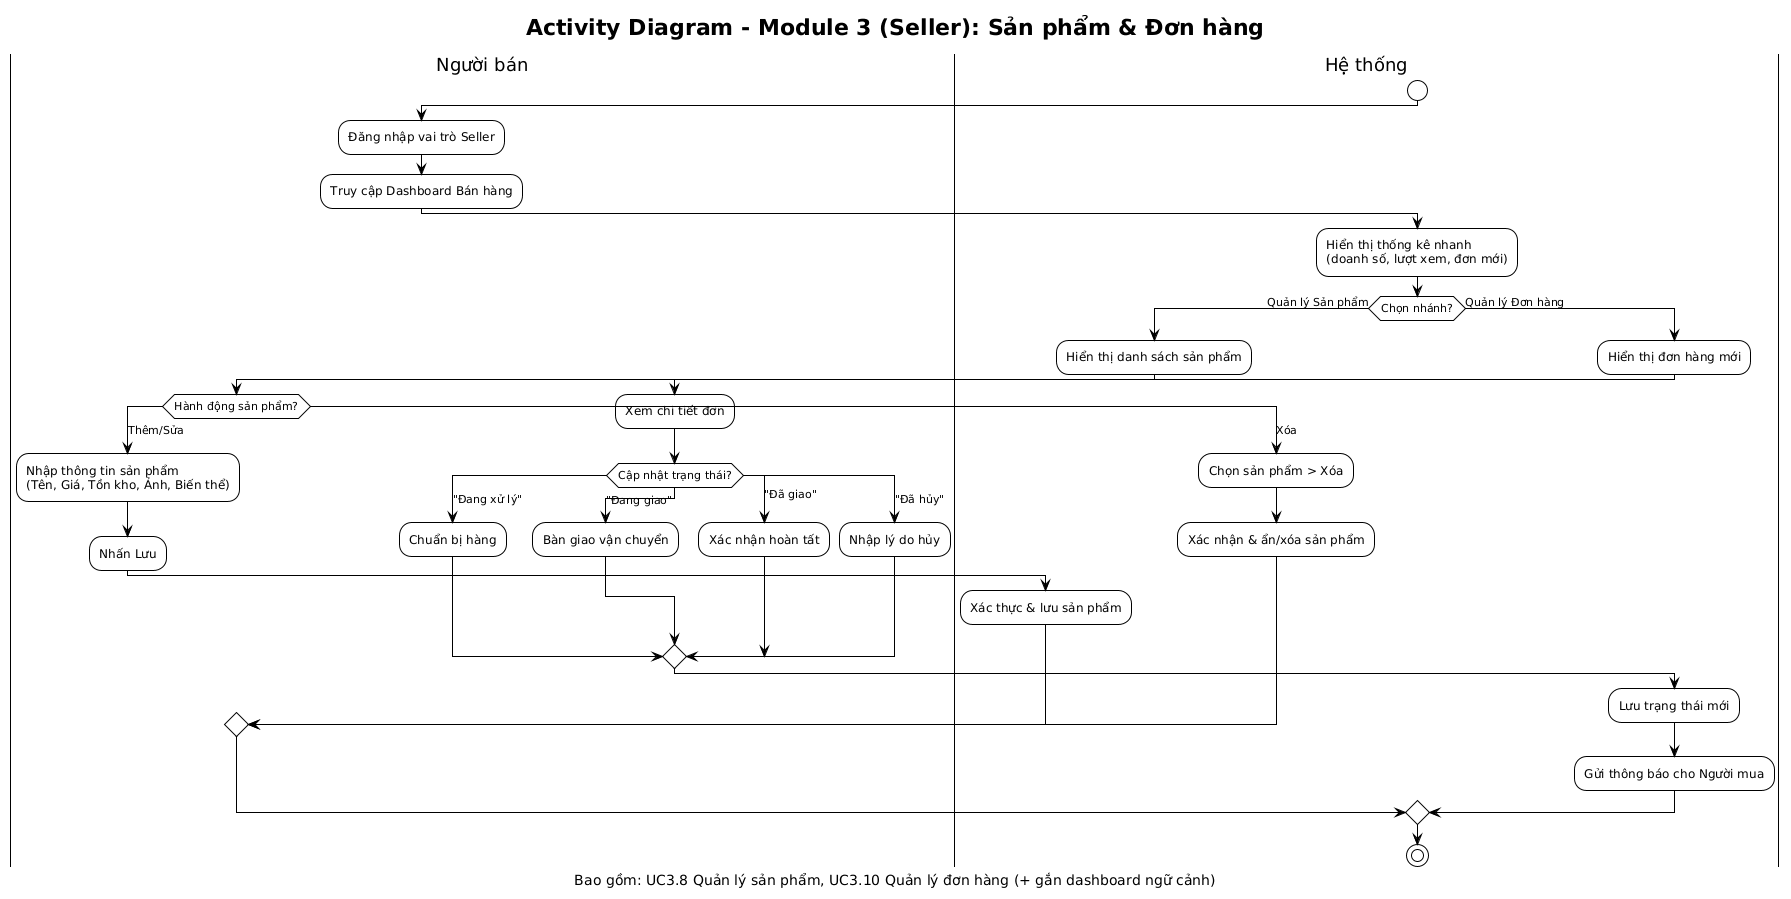
\includegraphics[width=\textwidth]{Images/Activity diagrams/AD-M3-Seller-ProductsOrders.png}
  \caption{Activity Diagram - Quản lý Sản phẩm và Đơn hàng của Seller (AD-M3-Seller-ProductsOrders)}
\end{figure}

\subsubsection{AD-M3-Seller-RefundReview}

Diagram này mô tả quy trình xử lý hoàn tiền và phản hồi đánh giá của Seller.

\textbf{UC3.11 – Xử lý hoàn tiền:} Seller chọn "Xử lý hoàn tiền", hệ thống hiển thị danh sách yêu cầu hoàn tiền. Seller xem chi tiết và quyết định chấp nhận hoặc từ chối. Nếu chấp nhận, hệ thống cập nhật trạng thái \textit{Refunded}, xử lý hoàn tiền và gửi thông báo. Nếu từ chối, hệ thống lưu lý do và gửi thông báo đến Buyer.

\textbf{UC3.12 – Phản hồi đánh giá:} Seller chọn "Đánh giá", hệ thống hiển thị danh sách đánh giá từ Buyer. Seller chọn đánh giá cần phản hồi, nhập nội dung và gửi. Hệ thống lưu phản hồi và hiển thị dưới đánh giá gốc trên trang sản phẩm.

\begin{figure}[H]
  \centering
  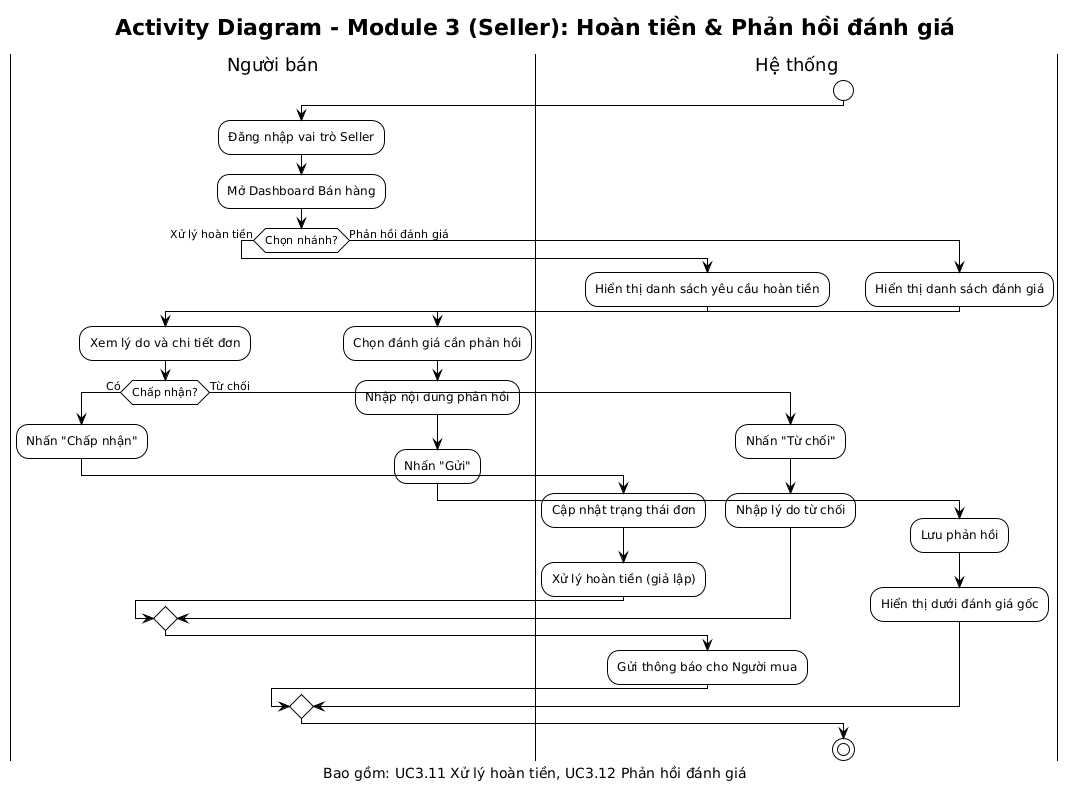
\includegraphics[width=\textwidth]{Images/Activity diagrams/AD-M3-Seller-RefundReview.png}
  \caption{Activity Diagram - Hoàn tiền và Phản hồi Đánh giá của Seller (AD-M3-Seller-RefundReview)}
\end{figure}

\subsection{Module 4 – Admin}

Module này cung cấp công cụ quản trị: quản lý tài khoản (vô hiệu hóa, kích hoạt, thay đổi vai trò), quản lý nội dung (duyệt và xóa bài đăng, sản phẩm vi phạm), xử lý báo cáo vi phạm, và thống kê tổng quan hệ thống.

\subsubsection{AD-M4-Admin-AccountsContent}

Diagram này mô tả quy trình quản lý tài khoản người dùng và nội dung của Admin.

\textbf{UC4.1 – Quản lý tài khoản:} Admin chọn "Quản lý Tài khoản", hệ thống hiển thị danh sách người dùng. Admin có thể tìm kiếm/lọc theo tên, email, vai trò, trạng thái. Admin có thể vô hiệu hóa, kích hoạt lại, hoặc đổi vai trò người dùng. Mỗi hành động được ghi lịch sử và cập nhật database.

\textbf{UC4.2 – Quản lý nội dung:} Admin chọn "Quản lý Nội dung", hệ thống hiển thị danh sách bài đăng và sản phẩm (có thể lọc theo loại, người đăng, trạng thái). Admin xem chi tiết và có thể xóa nội dung vi phạm. Hệ thống xóa/ẩn nội dung và gửi email thông báo đến chủ sở hữu.

\begin{figure}[H]
  \centering
  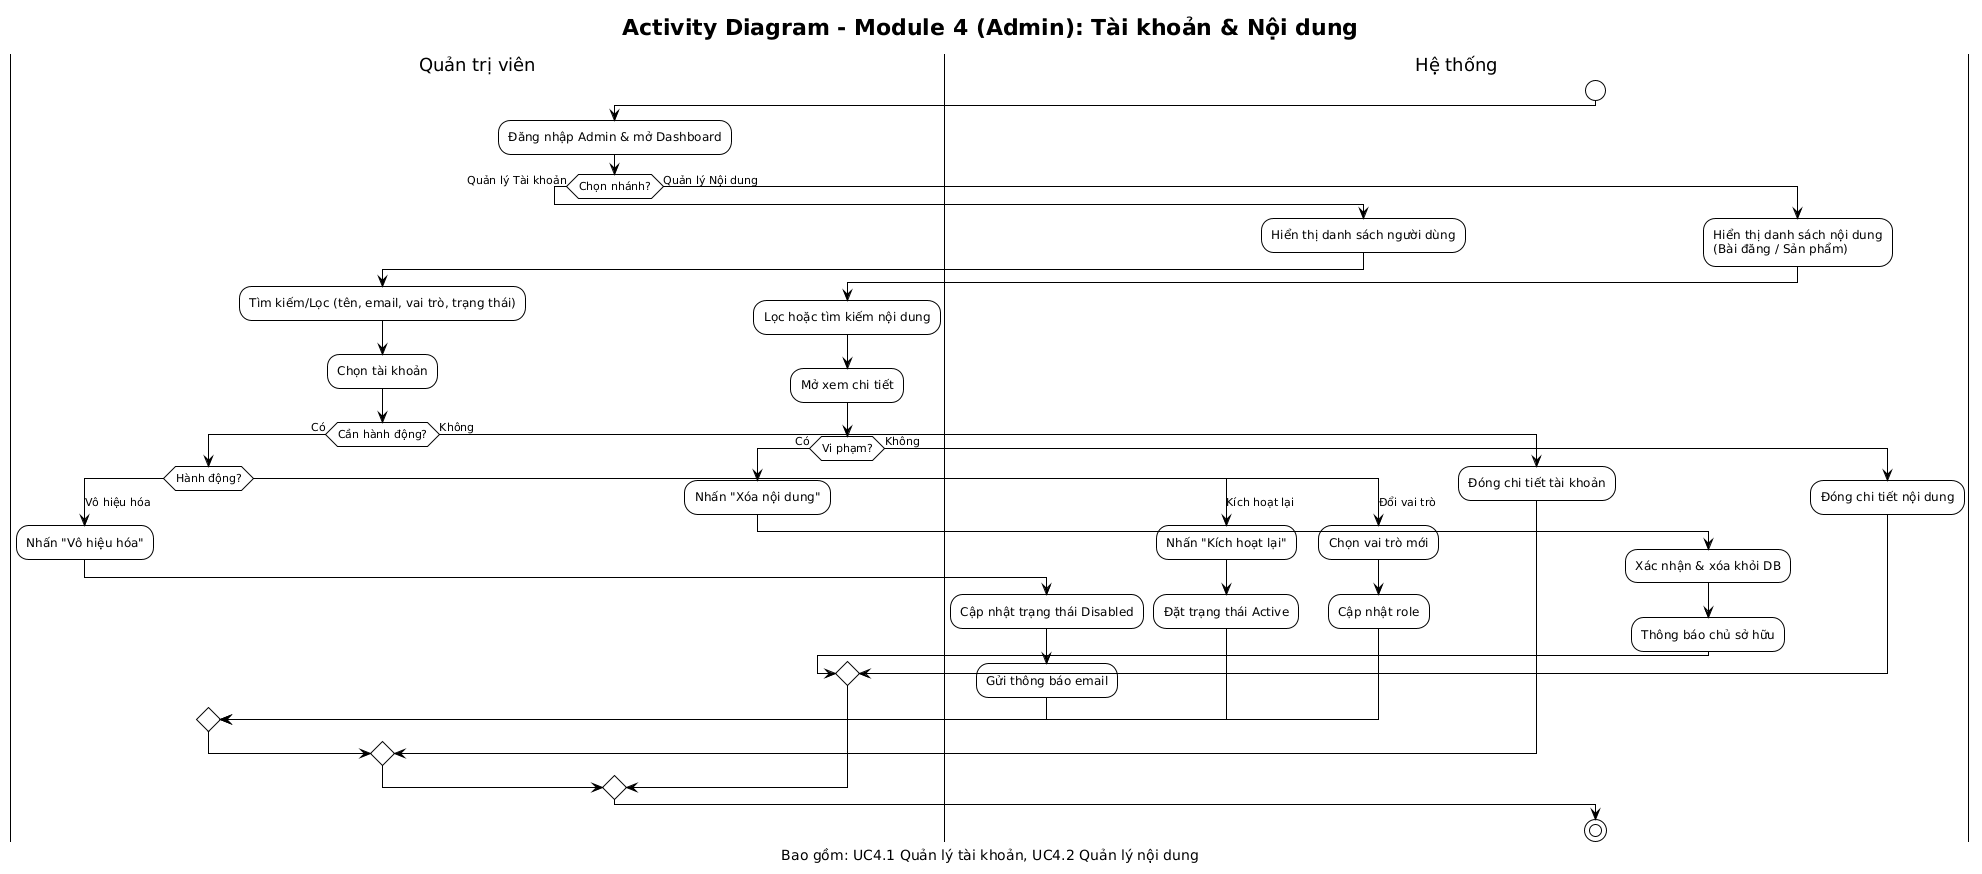
\includegraphics[width=\textwidth]{Images/Activity diagrams/AD-M4-Admin-AccountsContent.png}
  \caption{Activity Diagram - Quản lý Tài khoản và Nội dung của Admin (AD-M4-Admin-AccountsContent)}
\end{figure}

\subsubsection{AD-M4-Admin-ReportsAnalytics}

Diagram này mô tả quy trình xử lý báo cáo vi phạm và xem thống kê phân tích của Admin.

\textbf{UC4.3 – Xử lý báo cáo vi phạm:} Admin chọn "Xử lý báo cáo vi phạm", hệ thống hiển thị danh sách báo cáo đang chờ (sắp xếp theo mức độ ưu tiên). Admin xem chi tiết và đánh giá tính hợp lệ. Nếu hợp lệ, Admin chọn hành động: xóa nội dung, khóa tài khoản, hoặc gửi cảnh cáo. Hệ thống thực thi hành động, đánh dấu "Đã xử lý" và gửi thông báo. Nếu không hợp lệ, Admin đánh dấu "Từ chối".

\textbf{UC4.4 – Thống kê và phân tích:} Admin chọn khoảng thời gian và xem Dashboard với các chỉ số: số lượng người dùng (mới, tổng), tỷ lệ Buyer/Seller, số lượng bài đăng/sản phẩm mới, hoạt động giao dịch (đơn hàng, doanh thu). Dashboard có biểu đồ trực quan hóa xu hướng theo thời gian.

\begin{figure}[H]
  \centering
  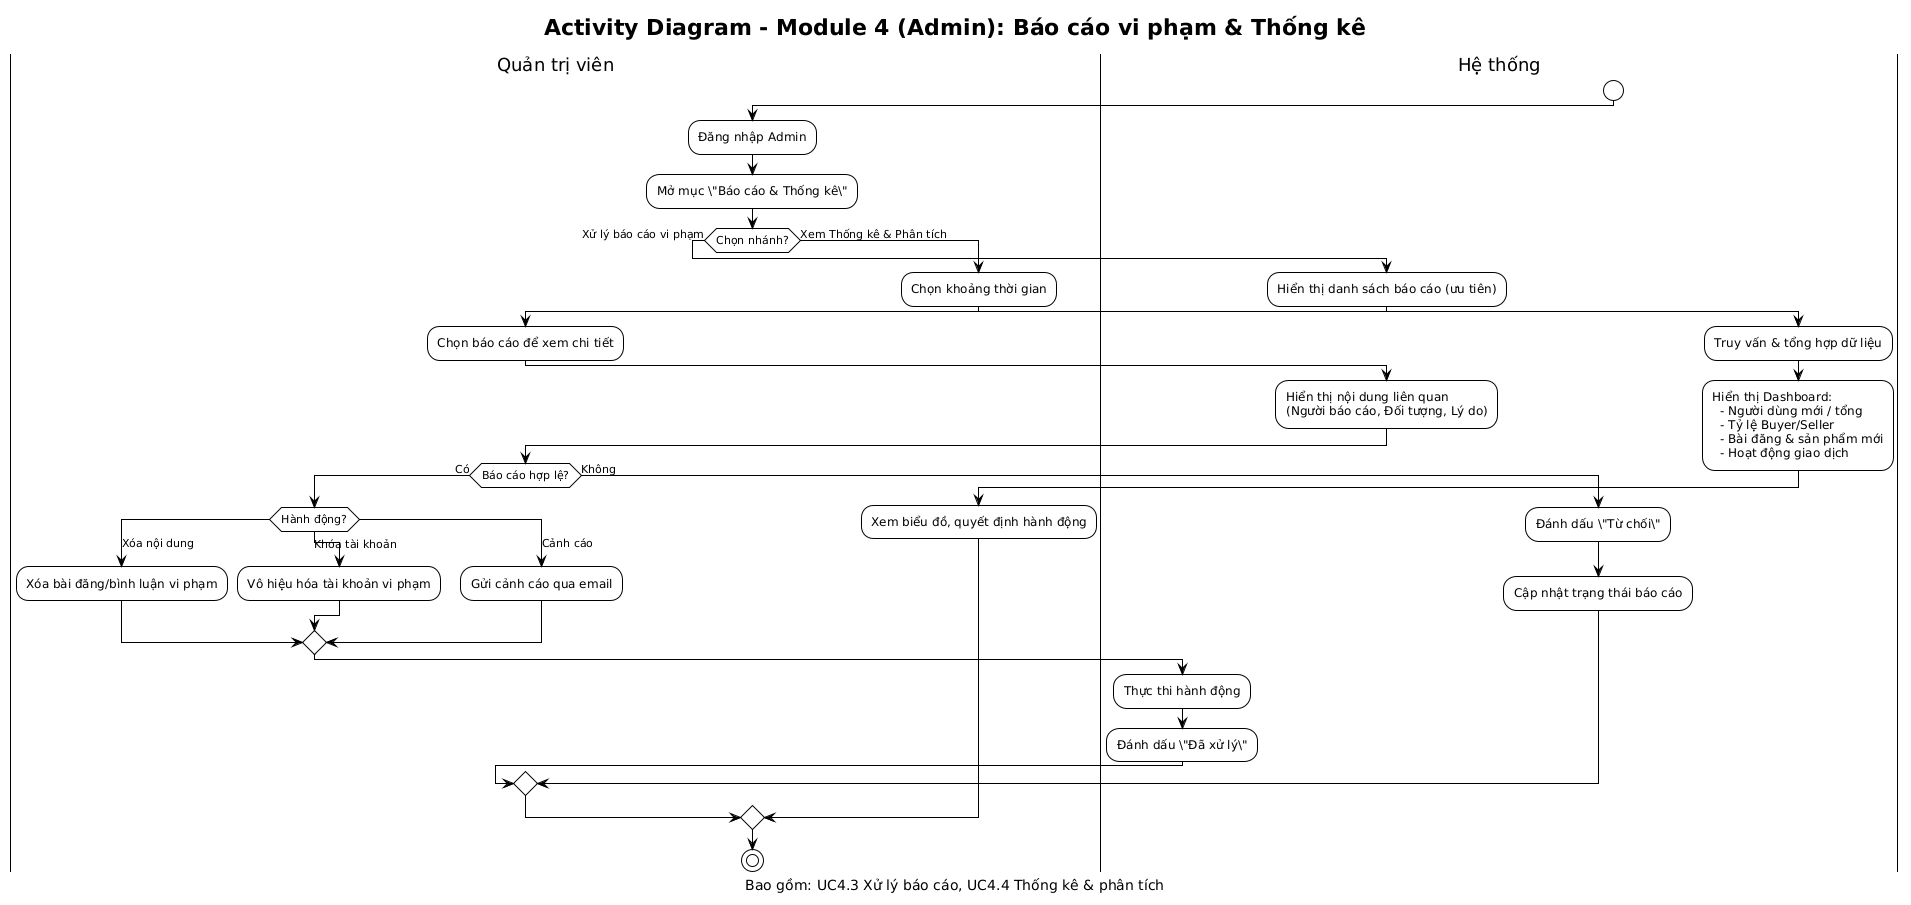
\includegraphics[width=\textwidth]{Images/Activity diagrams/AD-M4-Admin-ReportsAnalytics.png}
  \caption{Activity Diagram - Báo cáo và Thống kê của Admin (AD-M4-Admin-ReportsAnalytics)}
\end{figure}

\subsection{Module 5 – AI Content Assistant}

Module này tích hợp AI (Google Gemini API) để hỗ trợ tạo nội dung đa phương thức: generate text, generate image+text, và generate video+images+text. Luồng xử lý được thiết kế theo mô hình \textbf{Evaluate--Refine Loop}: sau khi gọi API tạo nội dung, hệ thống tự động đánh giá chất lượng kết quả dựa trên các tiêu chí đã định nghĩa. Nếu điểm đánh giá chưa đạt ngưỡng ($< 7.0/10$), hệ thống phân tích tiêu chí yếu, bổ sung ràng buộc vào prompt và gọi lại API (tối đa 3 lần). Kết quả tốt nhất được trả về cho người dùng kèm điểm đánh giá chi tiết và gợi ý chỉnh sửa.

\subsubsection{AD-M5-UC5.1-GenerateText}

Diagram này mô tả quy trình tạo nội dung bài đăng từ mô tả, ý tưởng và hình ảnh sản phẩm sử dụng Google Gemini API, bao gồm vòng lặp đánh giá và cải thiện tự động.

\textbf{UC5.1 – Tạo bài viết từ mô tả, ý tưởng và hình ảnh sản phẩm:} Người dùng nhập mô tả/ý tưởng và tải hình ảnh sản phẩm (nếu có), nhấn ``Tạo bài viết với AI''. Hệ thống thực hiện quy trình sau:

\begin{enumerate}
    \item \textbf{Phân tích đầu vào}: Trích xuất thực thể chính (tên sản phẩm, đặc điểm, lợi ích), xác định giọng điệu và phân loại loại nội dung (quảng cáo, chia sẻ, giáo dục). Nếu có hình ảnh, sử dụng Gemini Vision phân tích nội dung hình.
    \item \textbf{Xây dựng Prompt}: Tổng hợp thông tin vào prompt có cấu trúc 5 phần (System Instruction, Context, User Input, Constraints, Output Format). Ràng buộc bao gồm: độ dài 100--300 từ, 5--10 hashtag, phải có Call-to-Action, output dạng JSON.
    \item \textbf{Gọi API}: Gửi prompt đến Google Gemini API.
    \item \textbf{Đánh giá chất lượng}: Kết quả được chấm điểm theo 6 tiêu chí: Tính liên quan (0.25), Tính hấp dẫn (0.20), Cấu trúc hoàn chỉnh (0.15), Độ dài phù hợp (0.10), Chất lượng ngôn ngữ (0.15), Giá trị thương mại (0.15). Điểm tổng hợp là trung bình có trọng số.
    \item \textbf{Quyết định}: Nếu điểm $\geq$ 7.0 $\rightarrow$ trả kết quả. Nếu $<$ 7.0 và chưa đạt giới hạn 3 lần thử $\rightarrow$ xác định tiêu chí yếu, bổ sung ràng buộc vào prompt, gọi lại API. Nếu đã hết lần thử $\rightarrow$ trả kết quả tốt nhất kèm gợi ý chỉnh sửa.
    \item \textbf{Hiển thị}: Bài viết được chèn vào trình soạn thảo kèm điểm đánh giá chi tiết. Người dùng có thể chỉnh sửa trực tiếp, yêu cầu viết lại đoạn cụ thể, thay đổi giọng điệu, hoặc tạo lại toàn bộ.
\end{enumerate}

\begin{figure}[H]
  \centering
  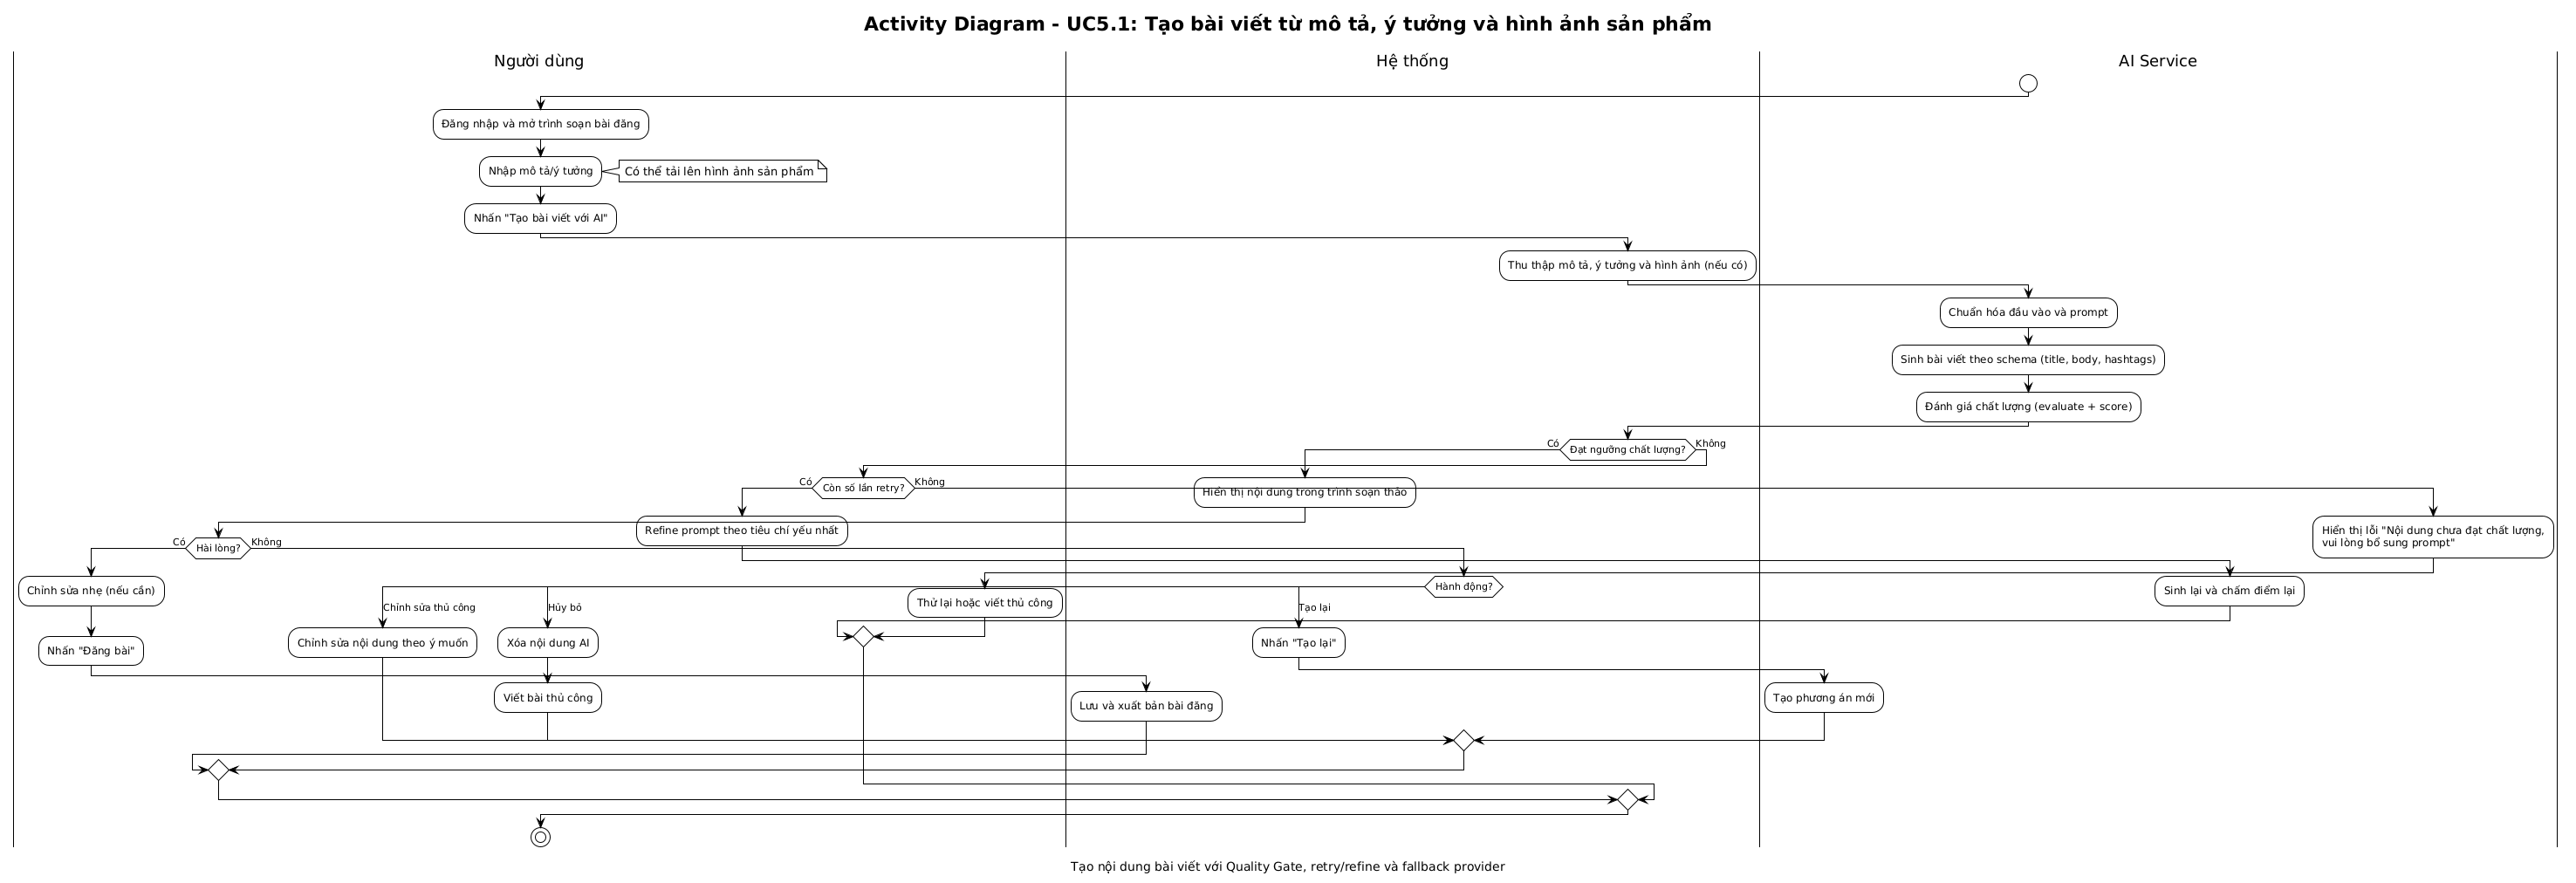
\includegraphics[width=\textwidth]{Images/Activity diagrams/AD-M5-UC5.1-GenerateText.png}
  \caption{Activity Diagram - Tạo bài viết với vòng lặp đánh giá và cải thiện (AD-M5-UC5.1-GenerateText)}
\end{figure}

\subsubsection{AD-M5-UC5.2-GenerateImageText}

Diagram này mô tả quy trình tạo bài viết và hình ảnh từ mô tả, ý tưởng và hình ảnh đầu vào sử dụng Google Gemini API, với đánh giá chất lượng riêng biệt cho text và image.

\textbf{UC5.2 – Tạo bài viết và hình ảnh:} Người dùng nhập mô tả/ý tưởng và hình ảnh đầu vào (nếu có), nhấn ``Tạo bài viết và hình ảnh với AI''. Hệ thống thực hiện quy trình sau:

\begin{enumerate}
    \item \textbf{Phân tích đầu vào}: Tương tự UC5.1, bổ sung phân tích hình ảnh đầu vào để xác định phong cách hình ảnh (màu sắc chủ đạo, bố cục, đối tượng).
    \item \textbf{Xây dựng Prompt kép}: Tạo prompt cho text (tương tự UC5.1) và prompt riêng cho image (bao gồm Visual Spec, phong cách, tỷ lệ 1:1 hoặc 4:5, negative prompt). Nội dung text vừa tạo được dùng làm context cho prompt image.
    \item \textbf{Gọi API}: Gửi prompt text đến Gemini API, sau đó sử dụng kết quả text làm context gửi prompt image.
    \item \textbf{Đánh giá chất lượng}: Text được đánh giá theo 6 tiêu chí (như UC5.1). Image được đánh giá theo 4 tiêu chí riêng: Tính liên quan (0.30), Chất lượng kỹ thuật (0.25), Tính thẩm mỹ (0.25), Nhất quán thương hiệu (0.20). Cả hai phải đạt ngưỡng $\geq$ 7.0/10.
    \item \textbf{Quyết định}: Nếu cả text và image đạt $\rightarrow$ trả kết quả. Nếu chỉ một phần chưa đạt $\rightarrow$ chỉ sửa prompt và tạo lại phần chưa đạt (không cần tạo lại phần đã tốt). Nếu hết lần thử $\rightarrow$ trả kết quả tốt nhất.
    \item \textbf{Hiển thị}: Bài viết và hình ảnh được hiển thị trong trình soạn thảo kèm điểm đánh giá từng loại. Người dùng có thể chỉnh sửa text, tạo lại hình ảnh với phong cách khác, hoặc tải lên hình ảnh thay thế.
\end{enumerate}

\begin{figure}[H]
  \centering
  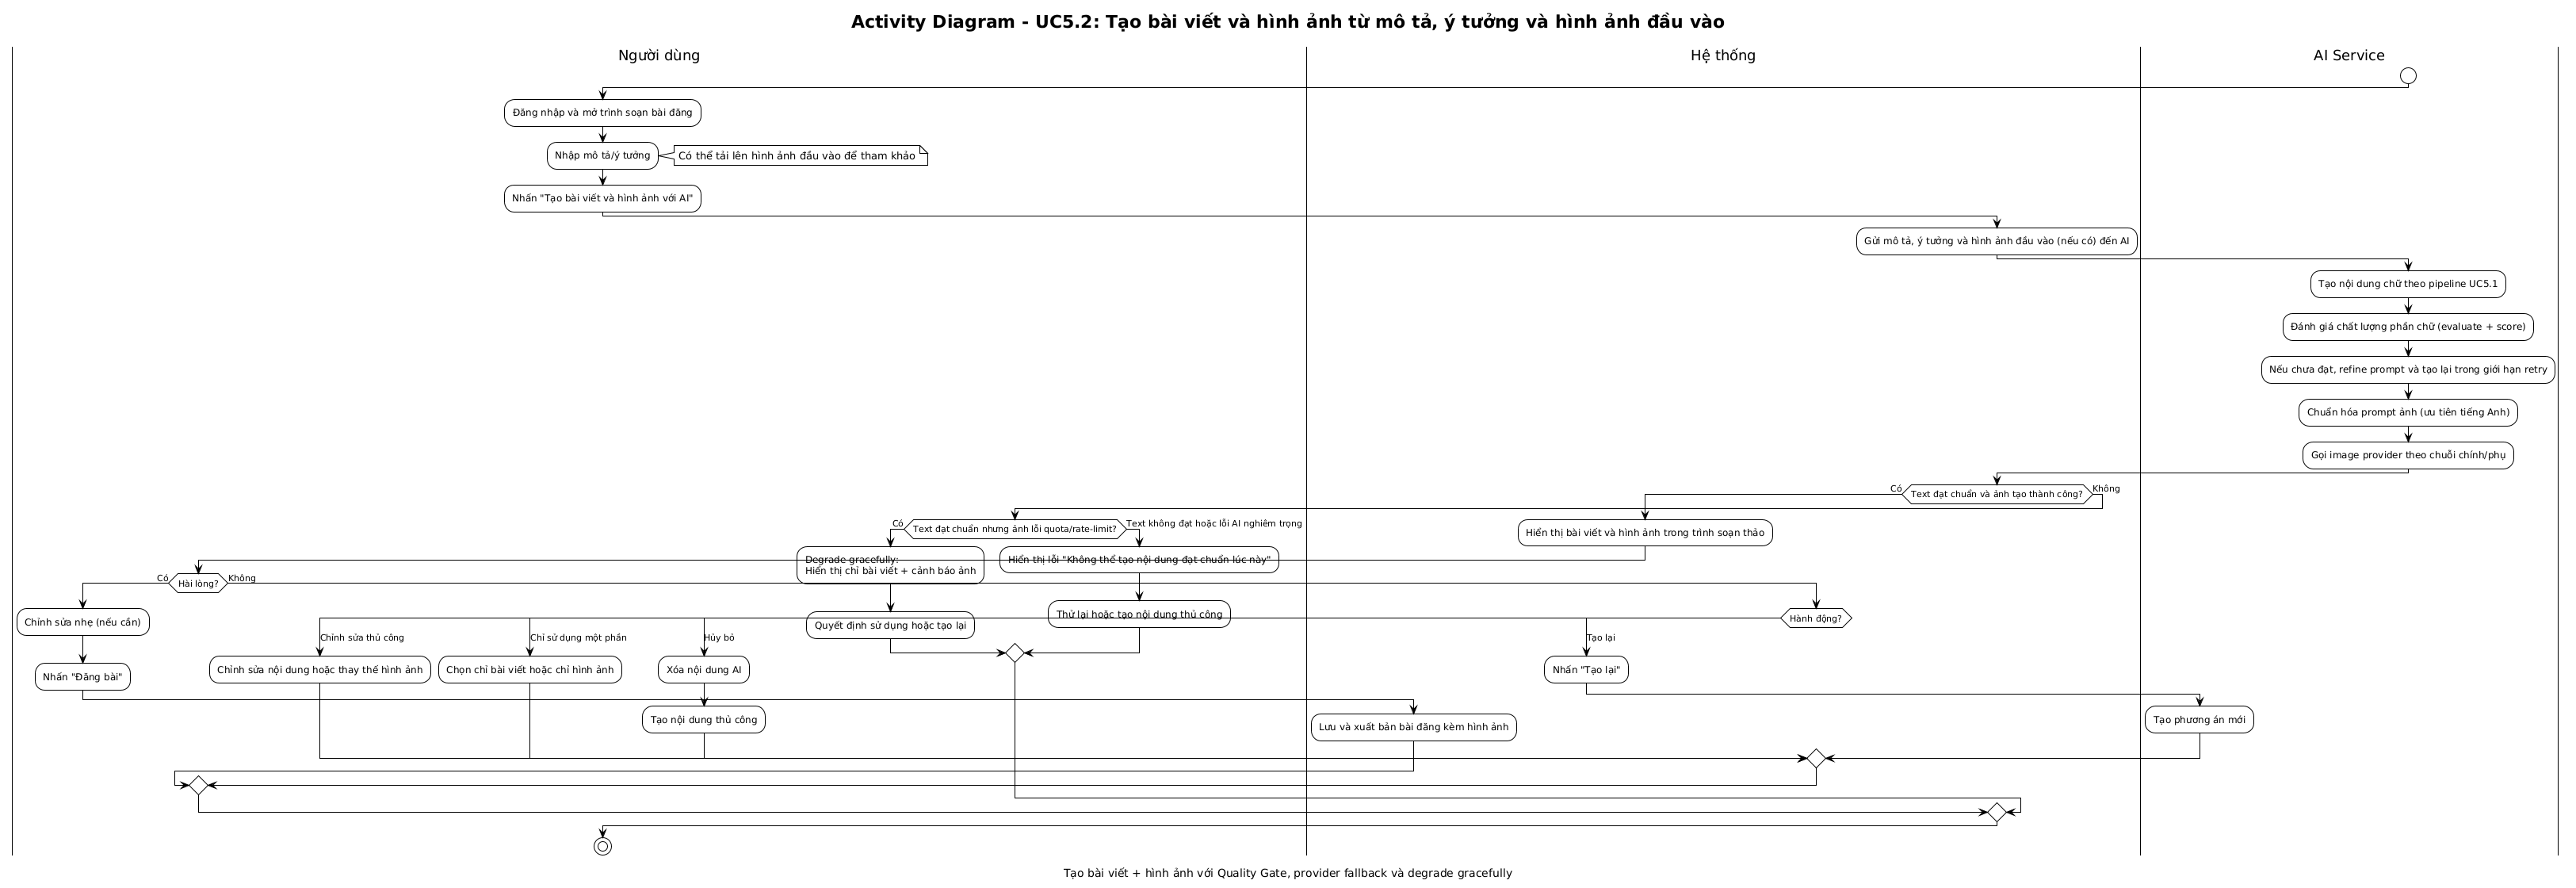
\includegraphics[width=\textwidth]{Images/Activity diagrams/AD-M5-UC5.2-GenerateImageText.png}
  \caption{Activity Diagram - Tạo bài viết và hình ảnh với đánh giá chất lượng riêng biệt (AD-M5-UC5.2-GenerateImageText)}
\end{figure}

\subsubsection{AD-M5-UC5.3-GenerateVideoImagesText}

Diagram này mô tả quy trình tạo nội dung đa phương thức (video + hình ảnh + bài viết) với pipeline đánh giá ba tầng.

\textbf{UC5.3 – Tạo video ngắn, hình ảnh và bài viết:} Người dùng nhập mô tả/ý tưởng và hình ảnh đầu vào (nếu có), nhấn ``Tạo video và nội dung đa phương thức với AI''. Hệ thống thực hiện quy trình sau:

\begin{enumerate}
    \item \textbf{Phân tích đầu vào}: Tương tự UC5.2, bổ sung xác định cấu trúc storyboard cho video (cảnh mở đầu, giới thiệu sản phẩm, highlight, CTA).
    \item \textbf{Xây dựng Prompt ba tầng}: Tạo prompt text $\rightarrow$ dùng text làm context tạo prompt image $\rightarrow$ dùng text + image làm context tạo prompt video. Prompt video bao gồm storyboard tự động, ràng buộc 15--30 giây, tỷ lệ 9:16 hoặc 1:1.
    \item \textbf{Gọi API tuần tự}: Gemini API cho text $\rightarrow$ Gemini API cho images (tối đa 3) $\rightarrow$ Google Veo 2 cho video.
    \item \textbf{Đánh giá chất lượng ba tầng}: Text (6 tiêu chí), Image (4 tiêu chí), Video (5 tiêu chí: Tính mạch lạc 0.25, Chất lượng hình ảnh 0.25, Độ dài phù hợp 0.15, Tính hấp dẫn 0.20, Nhất quán nội dung 0.15). Mỗi loại phải đạt $\geq$ 7.0/10.
    \item \textbf{Quyết định cải thiện có chọn lọc}: Chỉ tạo lại thành phần chưa đạt. Ví dụ: text và image đạt nhưng video chưa đạt $\rightarrow$ chỉ sửa prompt video và tạo lại video, giữ nguyên text và image. Tối đa 3 lần thử cho mỗi thành phần.
    \item \textbf{Hiển thị}: Video, hình ảnh và bài viết được hiển thị kèm điểm đánh giá từng loại. Người dùng có thể chỉnh sửa từng thành phần riêng biệt, tạo lại chỉ phần không hài lòng, hoặc thay thế bằng nội dung tự tạo.
\end{enumerate}

\begin{figure}[H]
  \centering
  \includegraphics[width=\textwidth]{Images/Activity diagrams/AD-M5-UC5.3-GenerateVideoImagesText.png}
  \caption{Activity Diagram - Tạo nội dung đa phương thức với pipeline đánh giá ba tầng (AD-M5-UC5.3-GenerateVideoImagesText)}
\end{figure}

\subsection{Module 6 – Post Scheduling}

Module này cho phép lên lịch đăng bài trong tương lai, quản lý bài đăng đã lên lịch (xem trước, chỉnh sửa, thay đổi thời gian, đăng ngay, xóa), và tự động xuất bản thông qua cron job.

\subsubsection{AD-M6-PostScheduling}

Diagram này mô tả quy trình lên lịch đăng bài và quản lý bài đăng đã lên lịch.

\textbf{UC6.1 – Lên lịch đăng bài:} Người dùng soạn bài đăng, chọn "Lên lịch" và chọn ngày/giờ xuất bản trong tương lai. Hệ thống kiểm tra thời gian hợp lệ, lưu bài đăng với trạng thái \textit{scheduled} và hiển thị thông báo. Nếu thời gian không hợp lệ, hệ thống báo lỗi.

\textbf{UC6.2 – Quản lý bài đăng đã lên lịch:} Người dùng xem danh sách bài viết chờ xuất bản. Người dùng có thể xem trước, chỉnh sửa nội dung/hình ảnh, thay đổi lịch đăng, đăng ngay, hoặc xóa bài viết. Mỗi hành động được cập nhật trong database ngay lập tức.

\textbf{Cron Job – Xuất bản tự động:} Cron job chạy định kỳ kiểm tra các bài viết có trạng thái \textit{scheduled} và thời gian xuất bản đã đến. Đối với mỗi bài viết đến hạn, cron job thay đổi trạng thái thành \textit{published}, xuất bản lên Feed và gửi thông báo đến tác giả.

\begin{figure}[H]
  \centering
  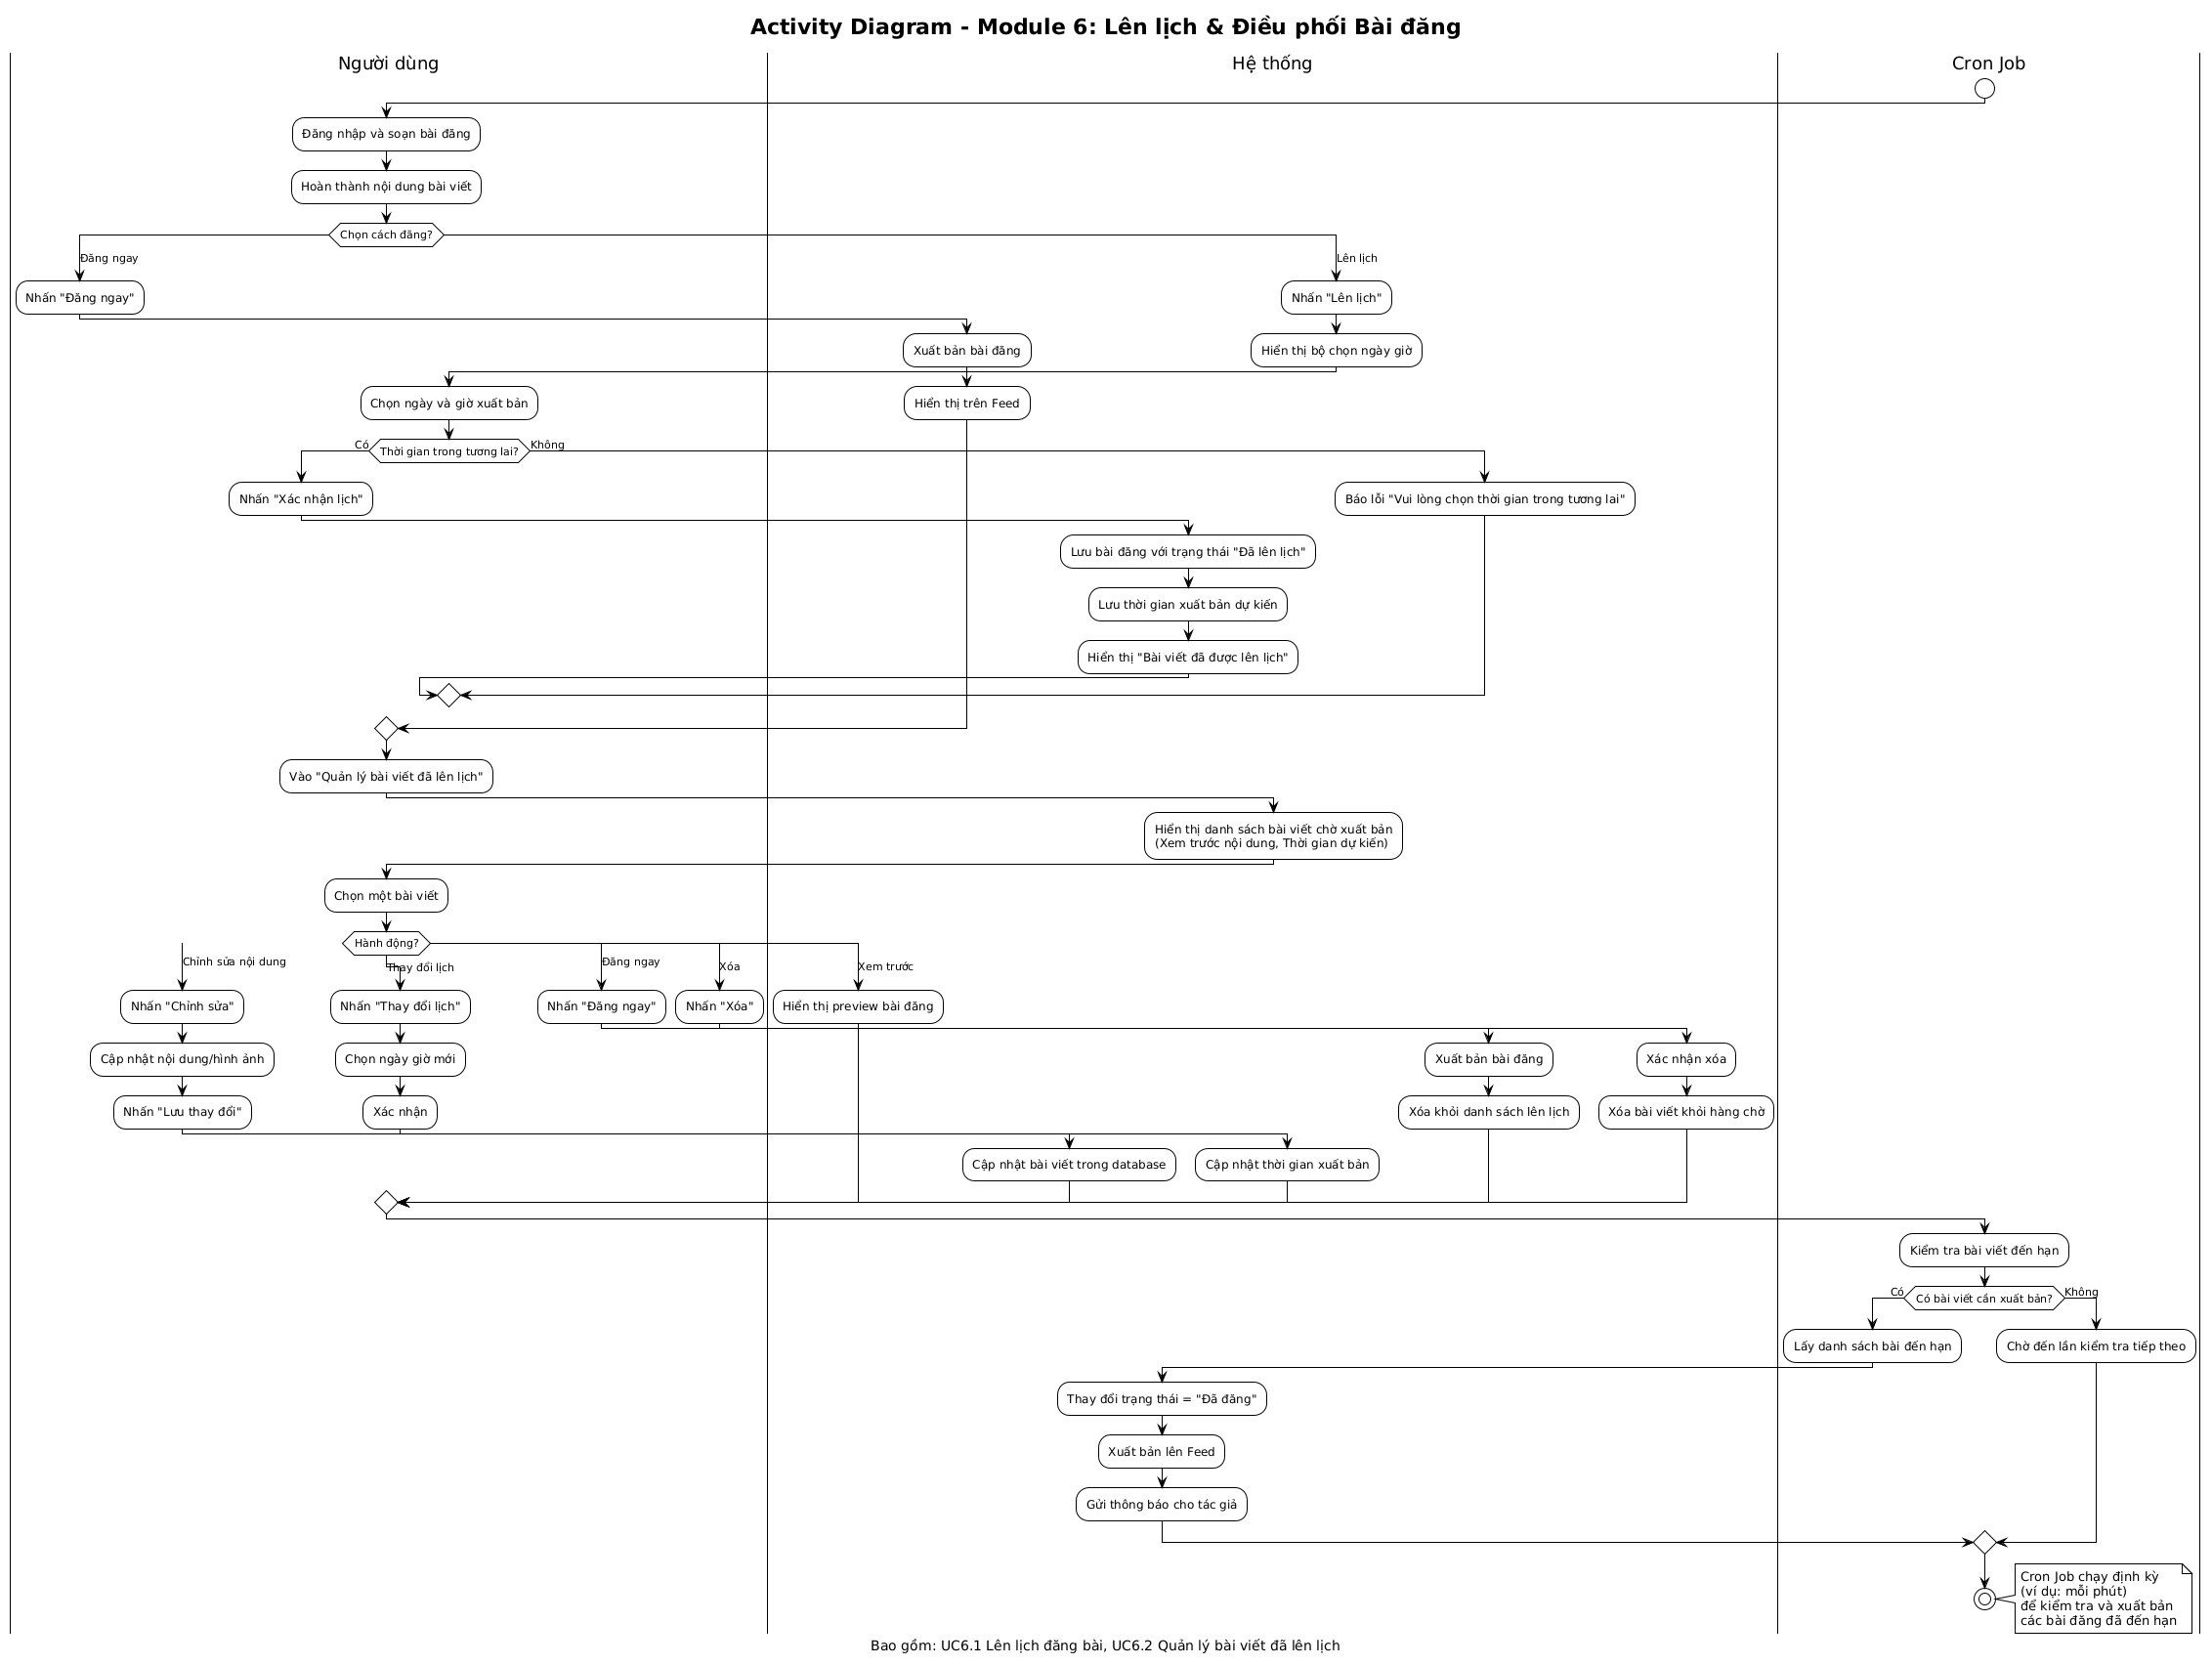
\includegraphics[width=\textwidth]{Images/Activity diagrams/AD-M6-PostScheduling.png}
  \caption{Activity Diagram - Lên lịch và Điều phối Bài đăng (AD-M6-PostScheduling)}
\end{figure}

\subsection{Module 7 – Notification}

Module này cung cấp hệ thống thông báo cho sự kiện tương tác xã hội (like, comment, follow, mention) và giao dịch (đơn hàng, hoàn tiền, đánh giá). Người dùng có thể quản lý thông báo (xem, đánh dấu đã đọc, xóa) và cấu hình nhận thông báo theo loại và kênh (web/email). Sử dụng WebSocket để gửi real-time khi online.

\subsubsection{AD-M7-NotificationSystem}

Diagram này mô tả toàn bộ hệ thống thông báo từ tạo, gửi, quản lý đến cấu hình.

\textbf{UC7.1 – Thông báo tương tác:} Khi A thực hiện tương tác với B (like, comment, follow, mention), hệ thống kiểm tra B có chặn A và cài đặt thông báo của B. Nếu cho phép, hệ thống tạo thông báo và lưu vào database. Nếu B đang online, gửi qua WebSocket ngay lập tức; nếu offline, lưu để hiển thị sau.

\textbf{UC7.2 – Thông báo giao dịch:} Hệ thống tạo và gửi thông báo cho các sự kiện: đơn hàng mới, xác nhận đơn, cập nhật trạng thái giao hàng, yêu cầu hoàn tiền, đánh giá mới. Tất cả thông báo được lưu vào database và gửi real-time nếu người nhận online và bật nhận loại thông báo này.

\textbf{UC7.3 – Quản lý thông báo:} Người dùng mở danh sách thông báo (sắp xếp theo thời gian, mới nhất ở trên). Người dùng có thể xem chi tiết, đánh dấu đã đọc (một hoặc tất cả), xóa một thông báo hoặc xóa tất cả (có xác nhận). Hệ thống cập nhật trạng thái và badge số thông báo chưa đọc.

\textbf{UC7.4 – Cài đặt thông báo:} Người dùng vào Cài đặt > Thông báo, bật/tắt từng loại thông báo (like, comment, follow, đơn hàng, đánh giá, tin nhắn, email) và chọn kênh nhận (web, email, hoặc cả hai). Hệ thống lưu cấu hình vào database và áp dụng ngay lập tức.

\begin{figure}[H]
  \centering
  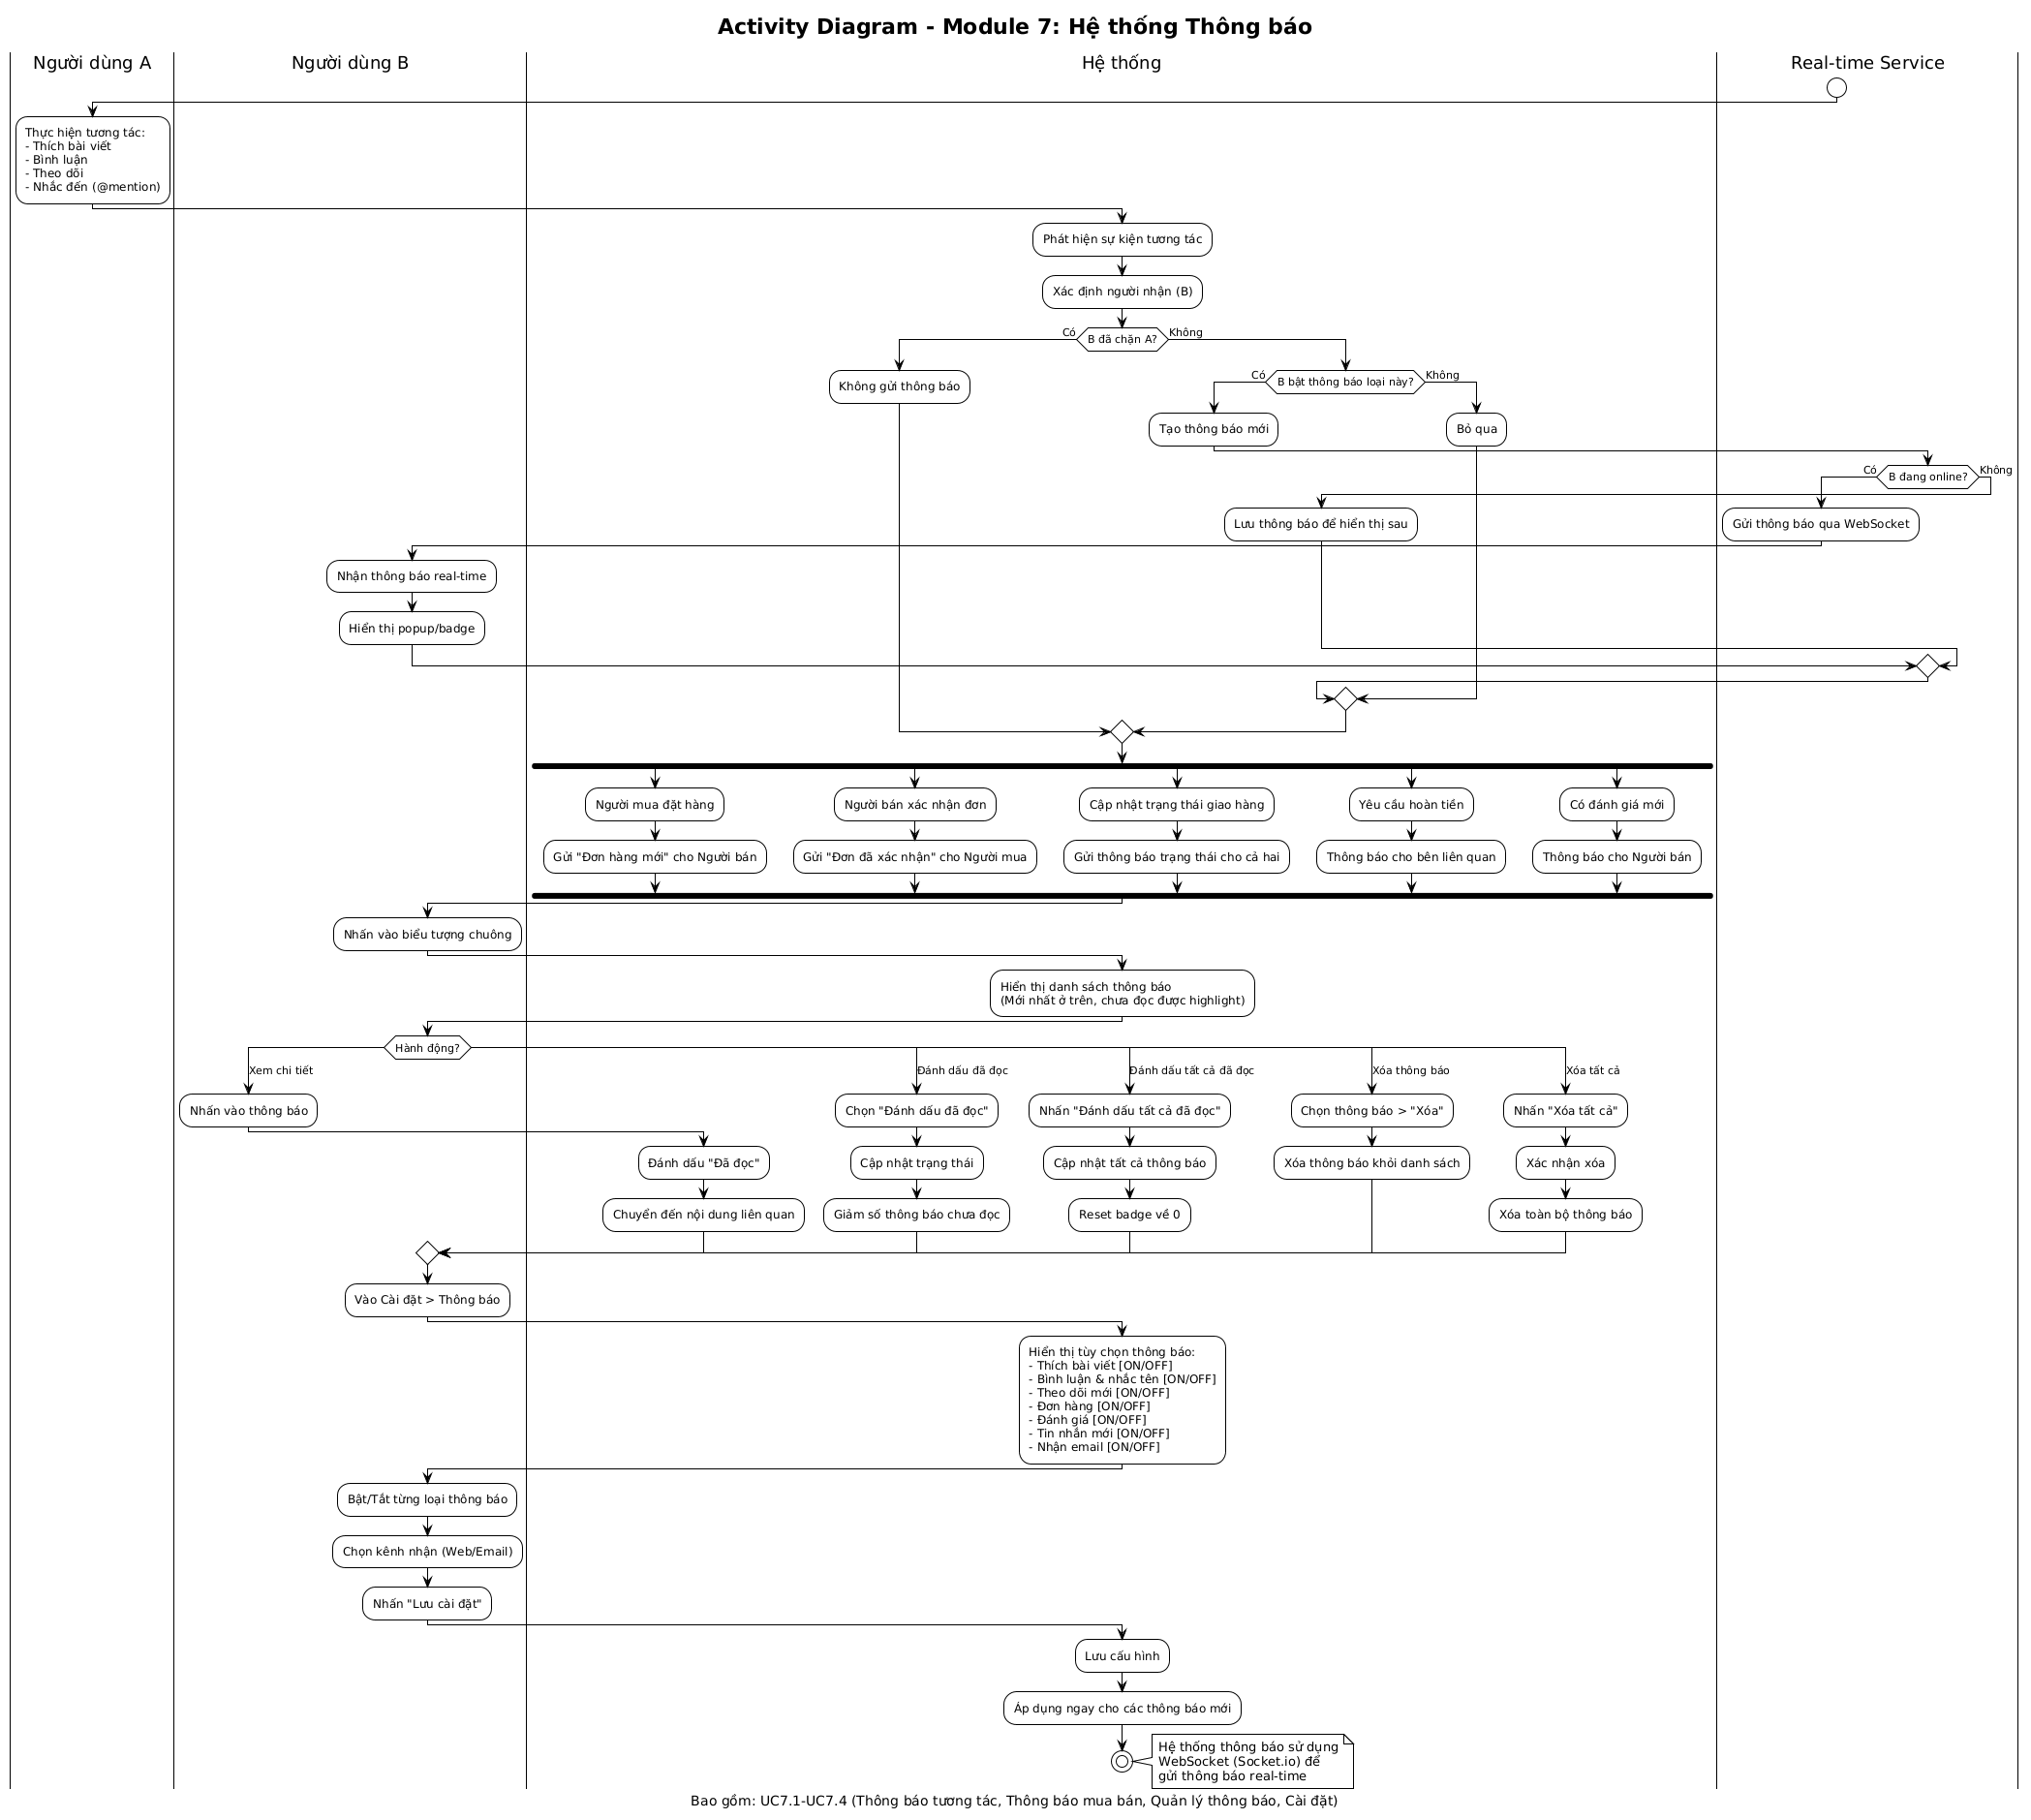
\includegraphics[width=\textwidth]{Images/Activity diagrams/AD-M7-NotificationSystem.png}
  \caption{Activity Diagram - Hệ thống Thông báo (AD-M7-NotificationSystem)}
\end{figure}


\section{Sequence diagram}
Phần này trình bày các Sequence Diagrams mô tả luồng tương tác giữa các thành phần hệ thống (Frontend, Controllers, Services, Database) thông qua các lời gọi API, kiểm tra điều kiện và phản hồi theo từng module. Mỗi module có mô tả tổng quan và các diagram chi tiết với hình ảnh minh họa.

\subsection{Module 1 – Quản lý Người dùng và Xác thực}

Module này mô tả luồng tương tác trong xác thực người dùng: đăng ký, đăng nhập với 2FA, khôi phục mật khẩu, quản lý hồ sơ, và nâng cấp lên Seller. Các diagram thể hiện cách Frontend giao tiếp với AuthController, UserController, EmailService và TokenService.

\subsubsection{SD-M1-Auth-RegisterLogin}

Diagram này mô tả chuỗi tương tác trong quá trình đăng ký và đăng nhập, bao gồm ba use case chính.

\textbf{UC1.1 – Đăng ký tài khoản:} Frontend gửi POST \texttt{/api/auth/register} với dữ liệu đăng ký. AuthController kiểm tra email đã tồn tại trong DB chưa. Nếu đã tồn tại, trả về 409 (Conflict). Nếu hợp lệ, AuthController tạo tài khoản với trạng thái \textit{unverified} và vai trò \textit{buyer}, gọi EmailService gửi email xác thực, và trả về 201 (Created).

\textbf{UC1.2 – Đăng nhập:} Frontend gửi POST \texttt{/api/auth/login} với email và mật khẩu. AuthController xác thực thông tin trong DB. Nếu sai/khóa/chưa xác thực, trả về 401/403. Nếu đúng và không bật 2FA, AuthController gọi TokenService tạo JWT, trả về 200 kèm token. Nếu bật 2FA, chuyển sang UC1.3.

\textbf{UC1.3 – Xác thực hai yếu tố (2FA):} AuthController gọi EmailService gửi mã OTP. Người dùng nhập mã OTP, Frontend gửi POST \texttt{/api/auth/verify-2fa}. AuthController kiểm tra mã OTP trong DB. Nếu hợp lệ, tạo JWT và trả về 200. Nếu sai/hết hạn, trả về 401.

\begin{figure}[H]
  \centering
  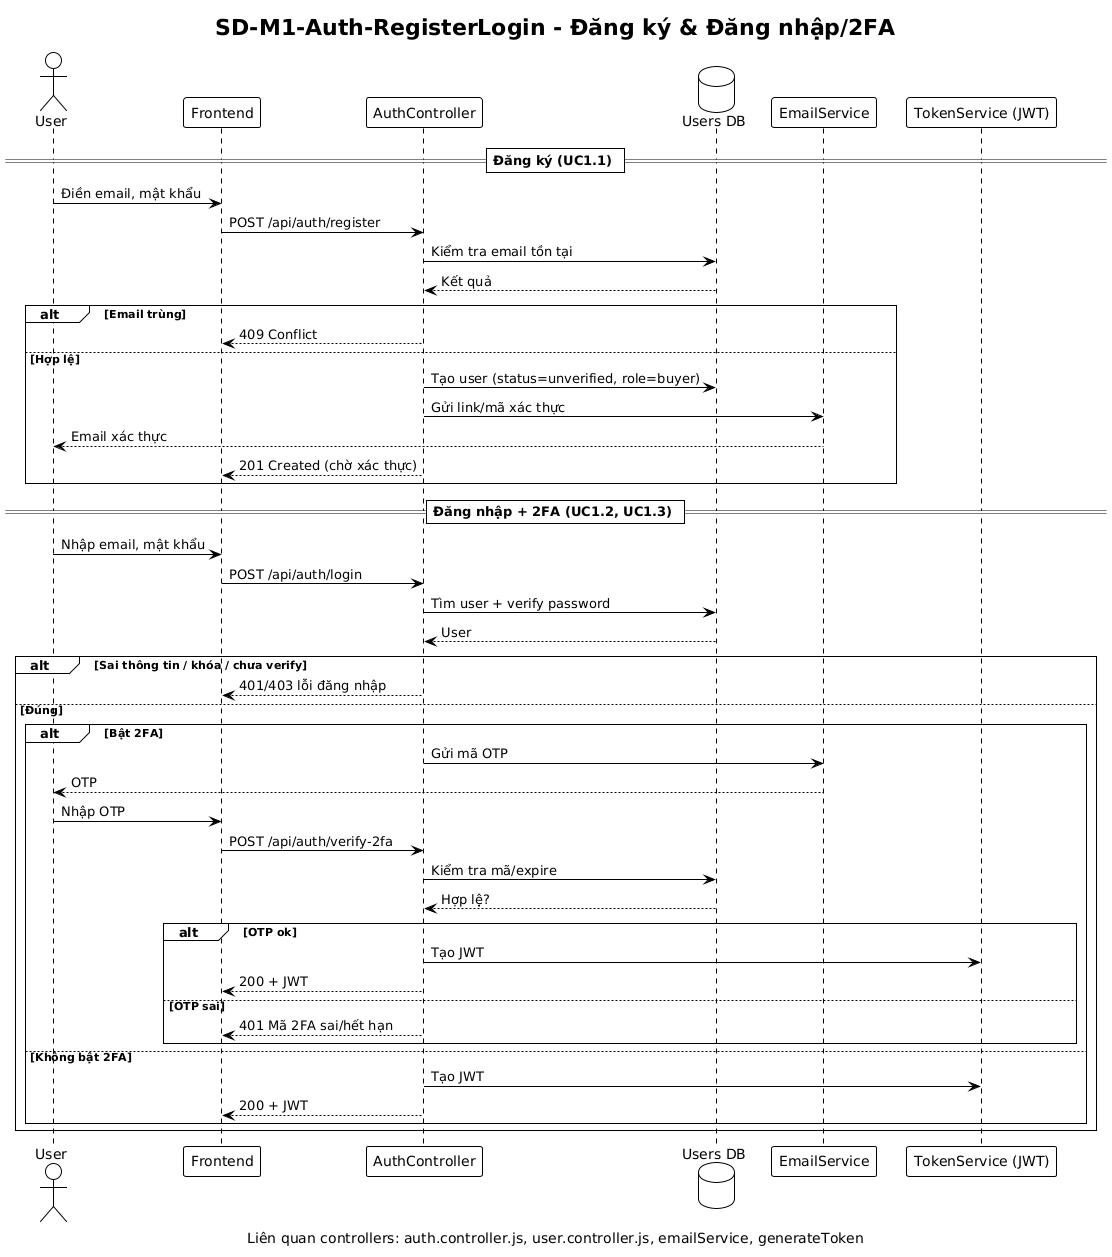
\includegraphics[width=\textwidth]{Images/Sequence diagrams/SD-M1-Auth-RegisterLogin.png}
  \caption{Sequence Diagram - Đăng ký và Đăng nhập (SD-M1-Auth-RegisterLogin)}
\end{figure}

\subsubsection{SD-M1-Auth-RecoveryLogout}

Diagram này mô tả chuỗi tương tác trong quá trình khôi phục mật khẩu và đăng xuất.

\textbf{UC1.4 – Khôi phục mật khẩu:} Frontend gửi POST \texttt{/api/auth/forgot-password} với email. AuthController xử lý yêu cầu theo cơ chế trả thông báo chung để tránh lộ thông tin tài khoản. Nếu email tồn tại, hệ thống tạo token reset, lưu vào DB và gọi EmailService gửi email. Người dùng mở link và đặt mật khẩu mới. Frontend gửi POST \texttt{/api/auth/reset-password} với token và mật khẩu mới. AuthController xác thực, hash mật khẩu và cập nhật trong DB, trả về 200.

\textbf{UC1.5 – Đăng xuất:} Frontend gửi POST \texttt{/api/auth/logout}. AuthController trả về kết quả đăng xuất, sau đó Frontend xóa token khỏi local storage và chuyển hướng về Trang chủ.

\begin{figure}[H]
  \centering
  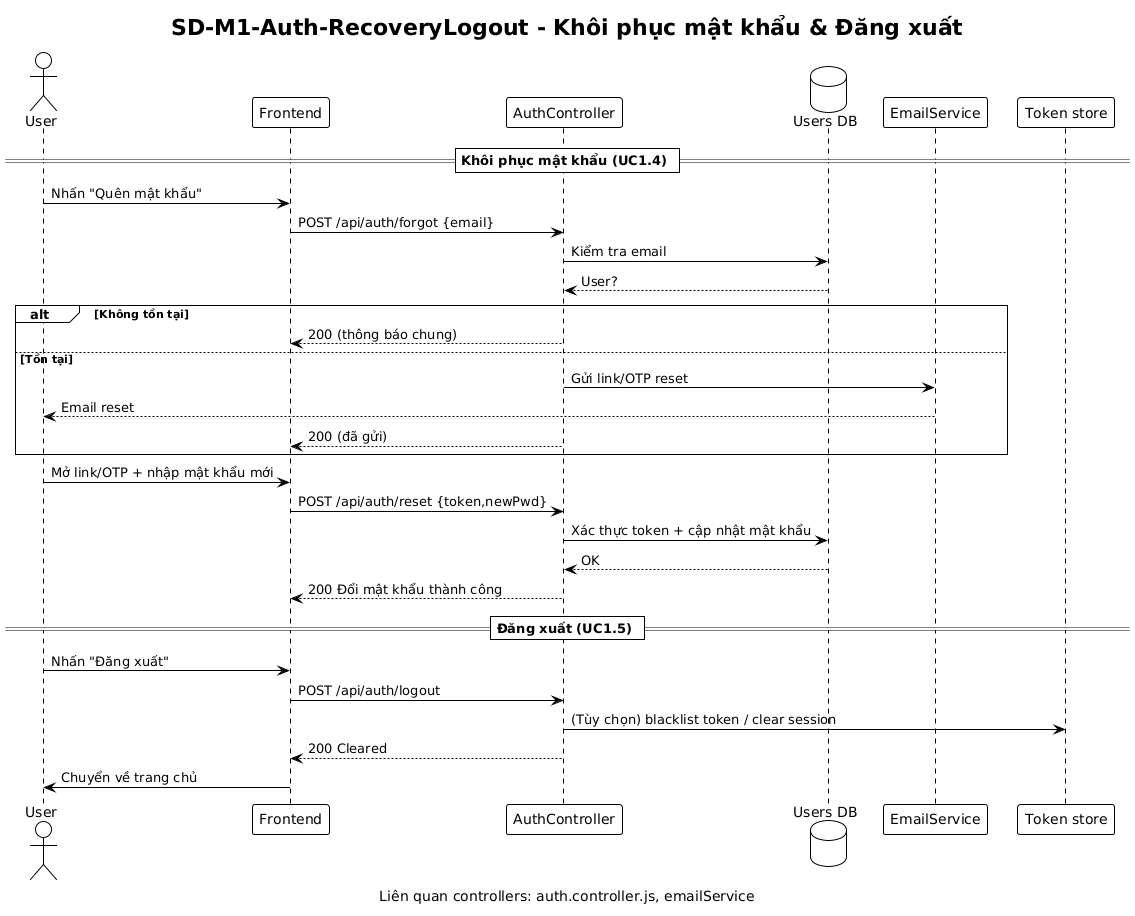
\includegraphics[width=\textwidth]{Images/Sequence diagrams/SD-M1-Auth-RecoveryLogout.png}
  \caption{Sequence Diagram - Khôi phục mật khẩu và Đăng xuất (SD-M1-Auth-RecoveryLogout)}
\end{figure}

\subsubsection{SD-M1-Profile-EditPrivacy}

Diagram này mô tả chuỗi tương tác trong quá trình chỉnh sửa hồ sơ và cài đặt quyền riêng tư.

\textbf{UC1.6 – Chỉnh sửa hồ sơ:} Frontend gửi PUT \texttt{/api/users/me} kèm dữ liệu cập nhật, file ảnh (nếu có) và JWT token. UserController xác thực token, nếu có ảnh thì gọi Storage service upload và nhận URL ảnh. UserController cập nhật thông tin trong Users DB, trả về 200 kèm hồ sơ mới.

\textbf{UC1.7 – Quyền riêng tư:} Frontend gửi PUT \texttt{/api/auth/privacy} kèm cấu hình quyền riêng tư và JWT token. AuthController xác thực token, lưu cấu hình vào Users DB và trả về 200.

\begin{figure}[H]
  \centering
  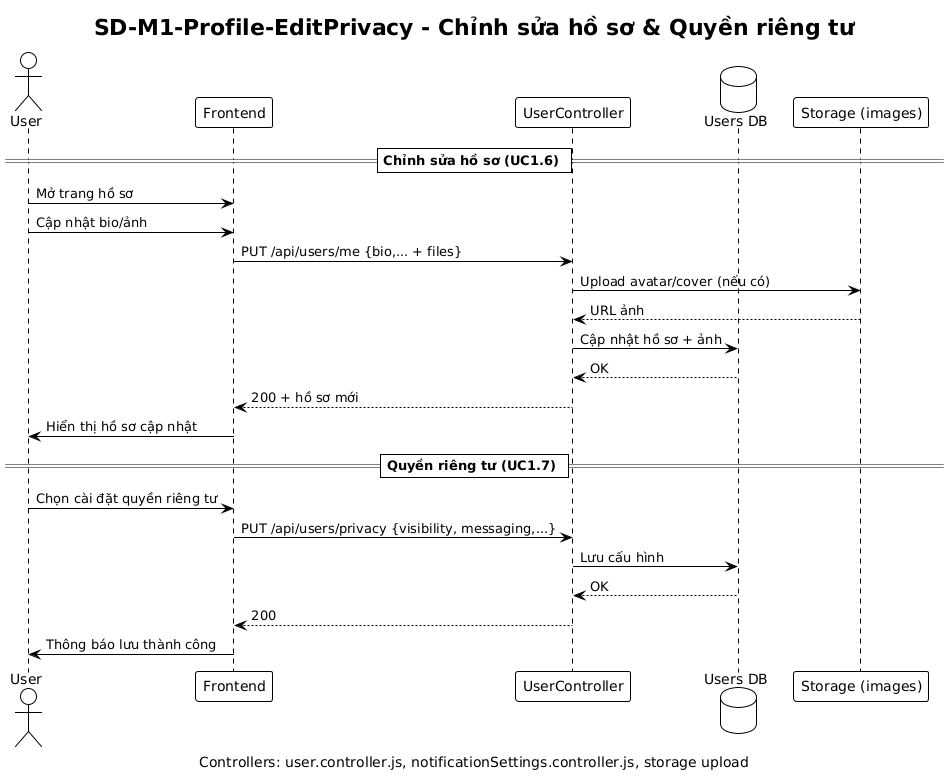
\includegraphics[width=\textwidth]{Images/Sequence diagrams/SD-M1-Profile-EditPrivacy.png}
  \caption{Sequence Diagram - Chỉnh sửa hồ sơ và Quyền riêng tư (SD-M1-Profile-EditPrivacy)}
\end{figure}

\subsubsection{SD-M1-Profile-SellerUpgrade}

Diagram này mô tả chuỗi tương tác trong quá trình đăng ký trở thành người bán.

\textbf{UC1.8 – Đăng ký Người bán:} Frontend gửi POST \texttt{/api/seller/apply} để khởi tạo hồ sơ, sau đó gửi dữ liệu qua các endpoint nhiều bước như \texttt{/api/seller/step1}, \texttt{/api/seller/step2}, \texttt{/api/seller/step3} hoặc \texttt{/api/seller/register-with-uploads}. SellerController xác thực, lưu hồ sơ vào bảng \textit{seller\_verifications} và chuyển trạng thái sang chờ duyệt. Admin xử lý qua admin API; nếu duyệt, hệ thống cập nhật role của user thành \textit{SELLER}.

\begin{figure}[H]
  \centering
  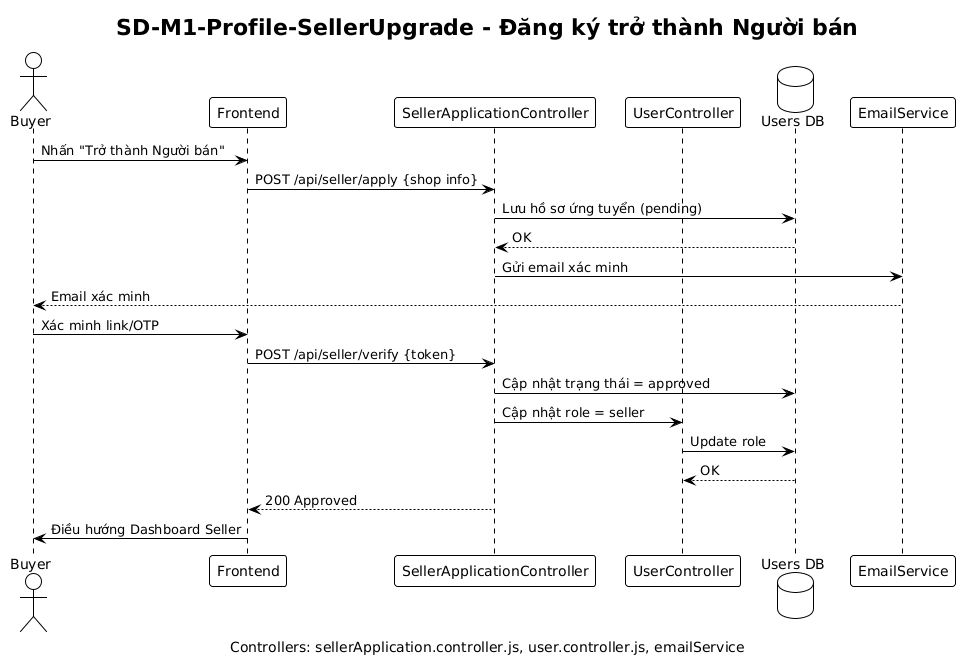
\includegraphics[width=\textwidth]{Images/Sequence diagrams/SD-M1-Profile-SellerUpgrade.png}
  \caption{Sequence Diagram - Đăng ký trở thành Người bán (SD-M1-Profile-SellerUpgrade)}
\end{figure}

\subsection{Module 2 – Tương tác Xã hội}

Module này mô tả luồng tương tác trong tính năng mạng xã hội: xem feed, tạo và tương tác với bài đăng, follow, nhắn tin, tham gia nhóm, báo cáo vi phạm. Các diagram thể hiện cách Frontend giao tiếp với PostController, UserController, MessageController, ReportController, FeedService, ProductController và NotificationService.

\subsubsection{SD-M2-FeedAndPosts}

Diagram này mô tả chuỗi tương tác trong quá trình xem feed, tạo bài đăng và tương tác với nội dung.

\textbf{UC2.1 – Xem Feed:} Frontend gửi GET \texttt{/api/posts/feed} kèm JWT token và tham số phân trang để lấy personalized feed, hoặc GET \texttt{/api/posts} cho feed công khai. PostController gọi PostService truy vấn DB lấy bài đăng từ người đang theo dõi kết hợp gợi ý, trả về danh sách đã sắp xếp. Frontend hiển thị với infinite scroll.

\textbf{UC2.2 và UC2.3 – Tạo bài đăng và gắn thẻ sản phẩm:} Nếu Seller muốn gắn sản phẩm, Frontend có thể lấy sản phẩm của seller qua các endpoint sản phẩm dành cho seller như \texttt{/api/products/seller/me}. Sau khi chọn một hoặc nhiều sản phẩm, Frontend gửi POST \texttt{/api/posts} kèm nội dung, media, mảng \texttt{productTags} và JWT token. PostController xác thực, kiểm tra nội dung, PostService lưu bài đăng vào \textit{posts} và lưu các tag vào \textit{post\_product\_tags}, sau đó trả về 201.

\textbf{UC2.4 – Tương tác với bài đăng:} Frontend gửi POST \texttt{/api/posts/:id/like} hoặc \texttt{/api/posts/:id/comments} kèm nội dung (nếu comment) và JWT token. PostController xác thực, lưu lượt thích/bình luận vào DB, gọi NotificationService gửi thông báo đến chủ sở hữu bài đăng, trả về 200 kèm trạng thái mới.

\begin{figure}[H]
  \centering
  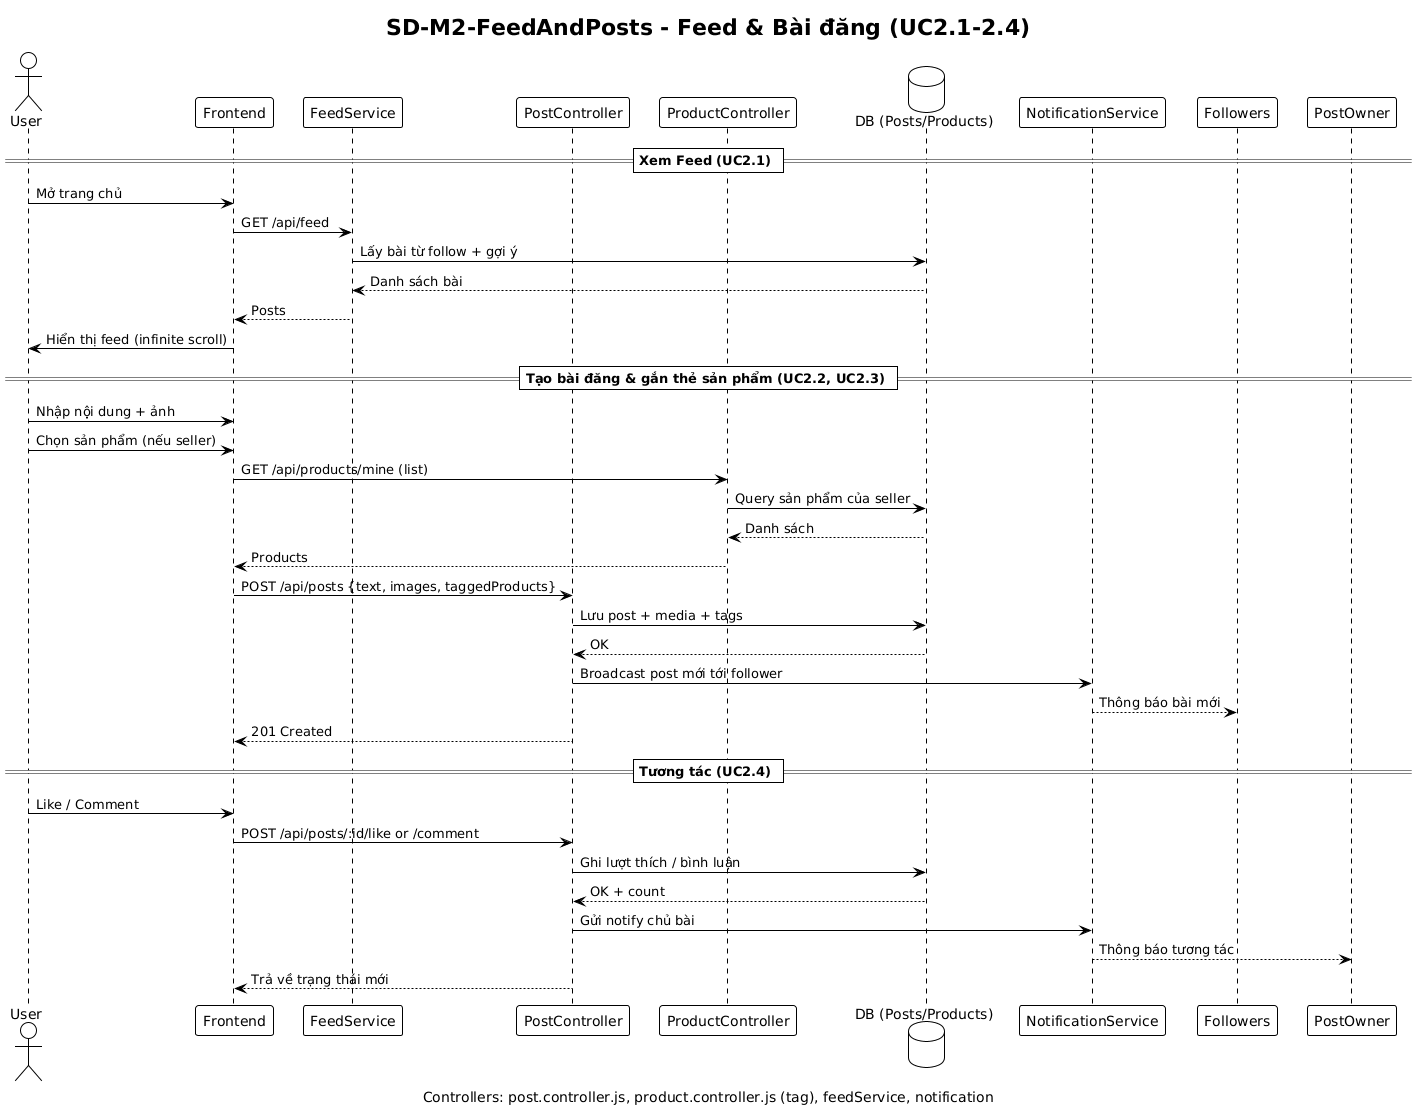
\includegraphics[width=\textwidth]{Images/Sequence diagrams/SD-M2-FeedAndPosts.png}
  \caption{Sequence Diagram - Feed và Bài đăng (SD-M2-FeedAndPosts)}
\end{figure}

\subsubsection{SD-M2-SocialConnections}

Diagram này mô tả chuỗi tương tác trong các kết nối xã hội giữa người dùng.

\textbf{UC2.5 – Theo dõi người dùng:} Frontend gửi POST \texttt{/api/users/:bId/follow} kèm JWT token. UserController xác thực, kiểm tra A chưa follow B, tạo mối quan hệ UserFollow trong DB, gọi NotificationService gửi thông báo đến B, trả về 200.

\textbf{UC2.6 – Nhắn tin 1-1:} Frontend gửi POST \texttt{/api/messages/conversations} để lấy hoặc tạo conversation với người nhận. Khi gửi tin nhắn, Frontend gửi POST \texttt{/api/messages/conversations/:conversationId} kèm nội dung và JWT token. MessageController xác thực người gửi thuộc conversation, lưu tin nhắn vào DB, emit realtime qua Socket.IO và tạo notification nếu người nhận offline.

\textbf{UC2.7 – Tham gia nhóm:} Frontend gửi POST \texttt{/api/groups/:groupId/join} kèm JWT token. GroupController xác thực, kiểm tra loại nhóm. Nếu công khai, thêm membership ngay; nếu riêng tư, tạo yêu cầu tham gia với trạng thái \textit{pending}. Lưu vào DB và trả về kết quả.

\textbf{UC2.8 – Báo cáo vi phạm:} Frontend gửi POST \texttt{/api/reports} kèm targetType, targetId, reason, description (nếu có) và JWT token. ReportController xác thực, lưu báo cáo với trạng thái \textit{pending} vào DB và trả về kết quả. Admin xem báo cáo qua admin API.

\begin{figure}[H]
  \centering
  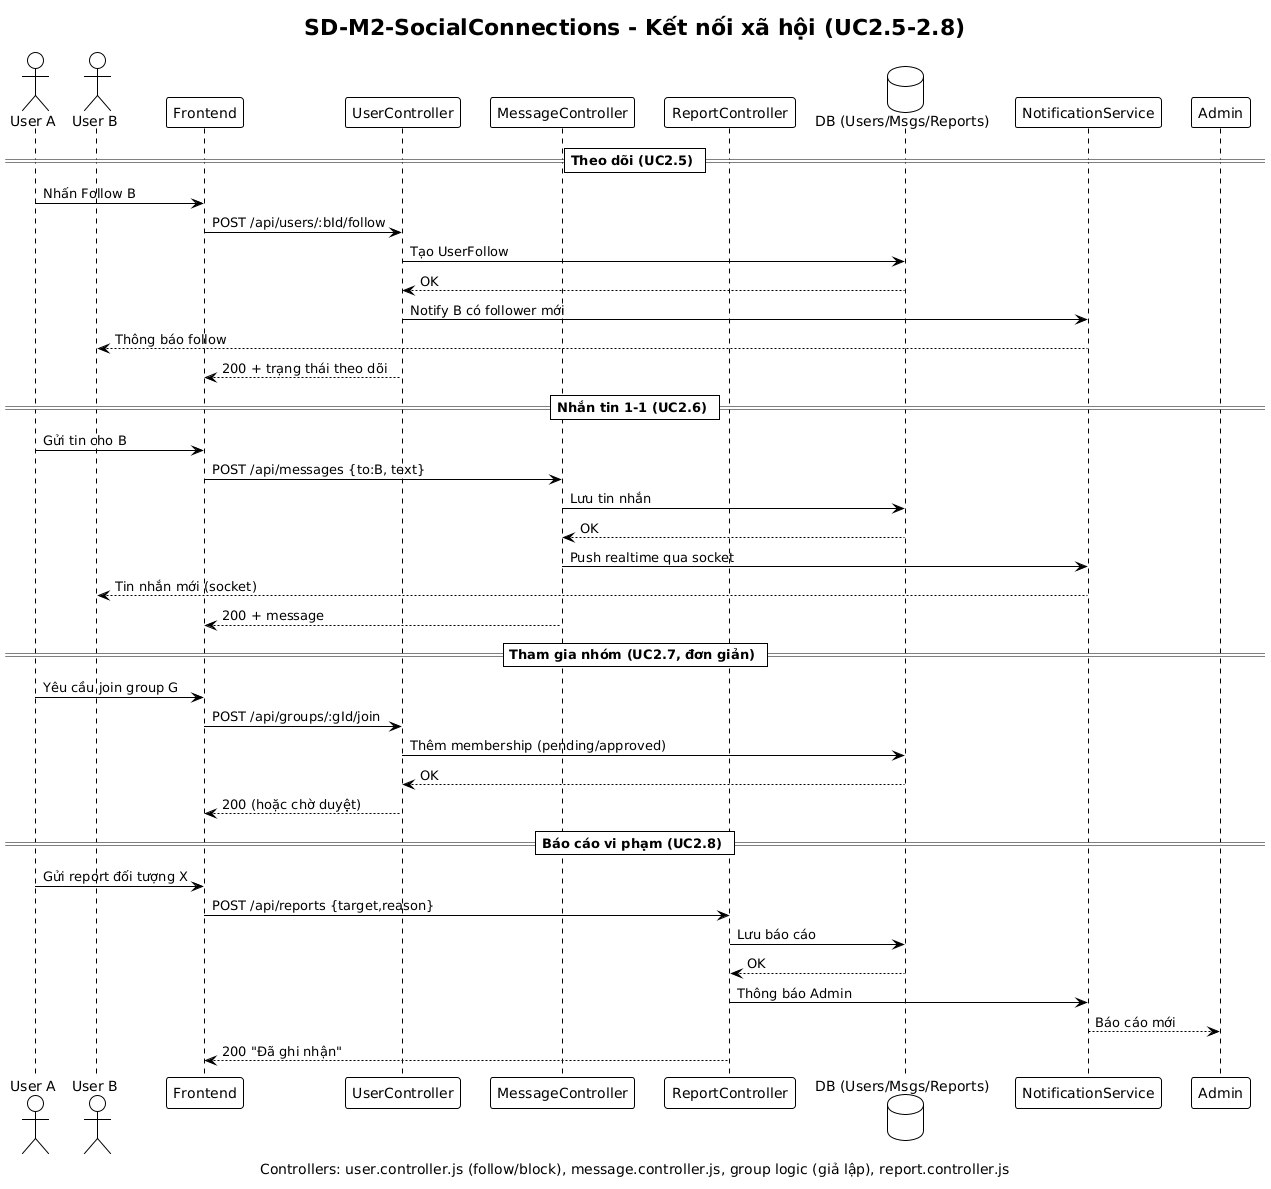
\includegraphics[width=\textwidth]{Images/Sequence diagrams/SD-M2-SocialConnections.png}
  \caption{Sequence Diagram - Kết nối Xã hội (SD-M2-SocialConnections)}
\end{figure}

\subsection{Module 3 – Hoạt động Thương mại}

Module này mô tả luồng tương tác trong hệ sinh thái thương mại: hành trình mua hàng của Buyer (tìm kiếm, xem sản phẩm, giỏ hàng, thanh toán, theo dõi đơn hàng, đánh giá) và tác vụ của Seller (quản lý sản phẩm, xử lý đơn hàng, hoàn tiền, phản hồi đánh giá). Các diagram thể hiện cách Frontend giao tiếp với ProductController, CartController, OrderController, ReviewController và NotificationService.

\subsubsection{SD-M3-BuyerFlow}

Diagram này mô tả chuỗi tương tác trong toàn bộ quy trình mua hàng từ góc nhìn của Buyer.

\textbf{UC3.1 và UC3.2 – Tìm kiếm và xem sản phẩm:} Frontend gửi GET \texttt{/api/products?query=...\&filters=...} với tham số tìm kiếm và lọc. ProductController truy vấn DB, trả về danh sách sản phẩm. Frontend hiển thị danh sách. Để xem chi tiết, Frontend gửi GET \texttt{/api/products/:id}. ProductController truy vấn DB lấy chi tiết và biến thể, trả về dữ liệu chi tiết.

\textbf{UC3.3 và UC3.4 – Quản lý giỏ hàng:} Frontend gửi POST \texttt{/api/cart/items} kèm ID sản phẩm, biến thể, số lượng và JWT token. CartController xác thực, kiểm tra tồn kho, lưu cart item vào DB, trả về giỏ hàng đã cập nhật. Để cập nhật/xóa: Frontend gửi PATCH \texttt{/api/cart/items/:id} hoặc DELETE. CartController cập nhật/xóa trong DB, tính lại tổng tiền, trả về giỏ hàng đã cập nhật.

\textbf{UC3.5 – Thanh toán:} Frontend gửi POST \texttt{/api/orders} kèm thông tin giỏ hàng, địa chỉ giao hàng, phương thức thanh toán và JWT token. OrderController xác thực, kiểm tra tồn kho. Nếu đủ hàng, tạo Order với trạng thái \textit{Processing} và OrderItems trong DB, gọi NotificationService gửi thông báo đến Seller, trả về 201. Nếu hết hàng, trả về 400.

\textbf{UC3.6 và UC3.7 – Theo dõi đơn hàng và đánh giá:} Frontend gửi GET \texttt{/api/orders/my/purchases} kèm JWT token. OrderController xác thực, truy vấn DB lấy danh sách đơn hàng của Buyer, trả về danh sách. Khi đơn hàng đã giao hoặc hoàn thành, Frontend gửi POST \texttt{/api/reviews} kèm ID order item, số sao, nhận xét, hình ảnh (nếu có) và JWT token. ReviewController xác thực, lưu đánh giá vào DB, trả về 201.

\begin{figure}[H]
  \centering
  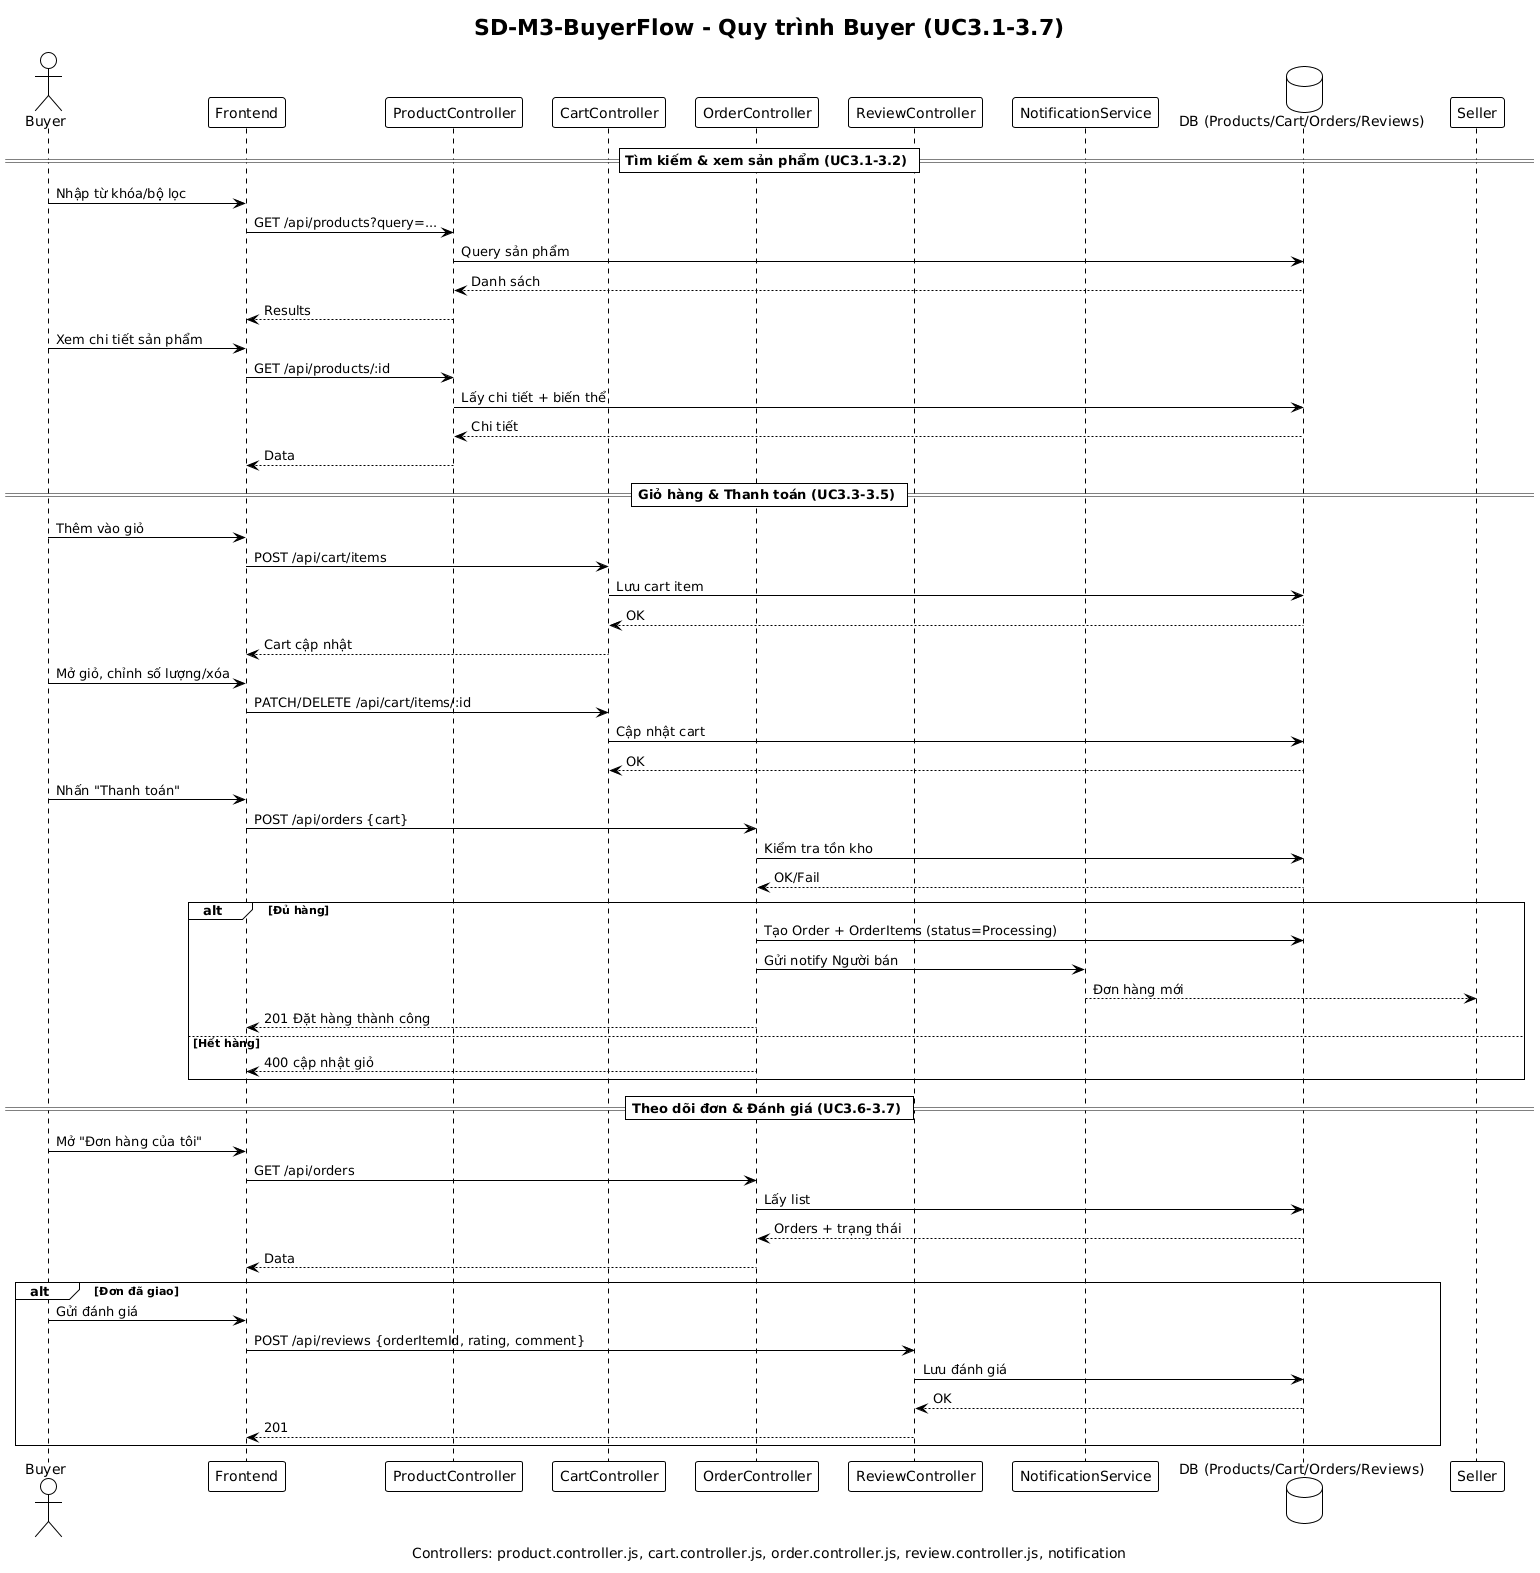
\includegraphics[width=\textwidth]{Images/Sequence diagrams/SD-M3-BuyerFlow.png}
  \caption{Sequence Diagram - Quy trình Mua hàng (SD-M3-BuyerFlow)}
\end{figure}

\subsubsection{SD-M3-Seller-ProductsOrders}

Diagram này mô tả chuỗi tương tác trong quá trình quản lý sản phẩm và đơn hàng của Seller.

\textbf{UC3.8 – Quản lý sản phẩm:} Frontend gửi POST \texttt{/api/products} (thêm), PUT \texttt{/api/products/:id} (sửa), hoặc DELETE \texttt{/api/products/:id} (xóa) kèm dữ liệu sản phẩm và JWT token. ProductController xác thực token và vai trò Seller, thực hiện lưu/cập nhật/soft-delete sản phẩm cùng biến thể trong DB, trả về 200/201.

\textbf{UC3.10 – Quản lý đơn hàng:} Frontend gửi GET \texttt{/api/orders/my/sales} kèm JWT token. OrderController xác thực token và vai trò Seller, truy vấn DB lấy danh sách đơn hàng của shop, trả về danh sách. Để cập nhật trạng thái: Frontend gửi PUT \texttt{/api/orders/:orderId/status} kèm trạng thái mới và JWT token. OrderController xác thực quyền, cập nhật trạng thái trong DB, gọi NotificationService thông báo Buyer, trả về 200.

\begin{figure}[H]
  \centering
  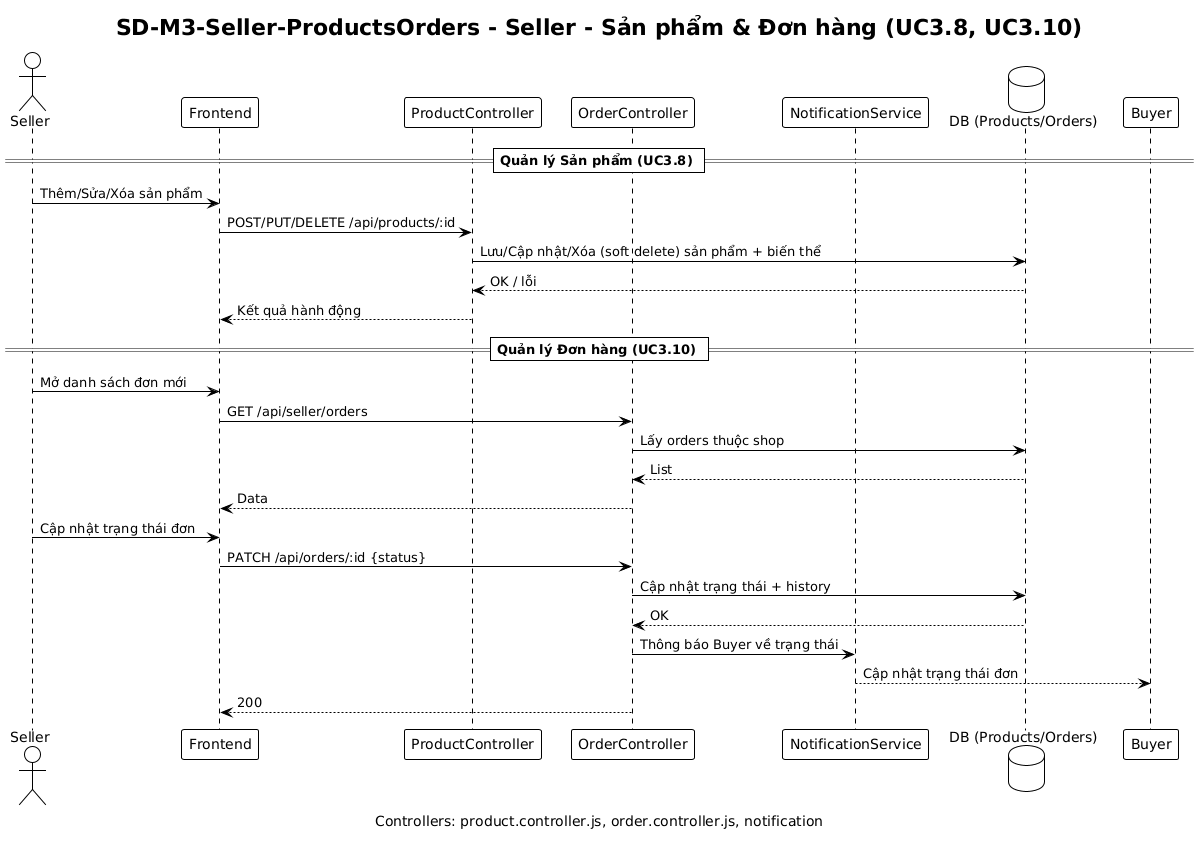
\includegraphics[width=\textwidth]{Images/Sequence diagrams/SD-M3-Seller-ProductsOrders.png}
  \caption{Sequence Diagram - Quản lý Sản phẩm và Đơn hàng của Seller (SD-M3-Seller-ProductsOrders)}
\end{figure}

\subsubsection{SD-M3-Seller-RefundReview}

Diagram này mô tả chuỗi tương tác trong quá trình xử lý hoàn tiền và phản hồi đánh giá của Seller.

\textbf{UC3.11 – Xử lý hoàn tiền:} Frontend gửi GET \texttt{/api/orders/seller/refunds} kèm JWT token. OrderController xác thực, truy vấn DB lấy danh sách yêu cầu hoàn tiền, trả về danh sách. Seller quyết định: Frontend gửi POST \texttt{/api/orders/:orderId/refund} kèm quyết định và lý do. OrderController cập nhật trạng thái/lý do liên quan trong phạm vi giả lập, gọi NotificationService thông báo Buyer và trả về kết quả.

\textbf{UC3.12 – Phản hồi đánh giá:} Frontend gửi POST \texttt{/api/reviews/:id/reply} kèm nội dung phản hồi và JWT token. ReviewController xác thực token và vai trò Seller, lưu phản hồi vào DB, gọi NotificationService thông báo Buyer, trả về 201.

\begin{figure}[H]
  \centering
  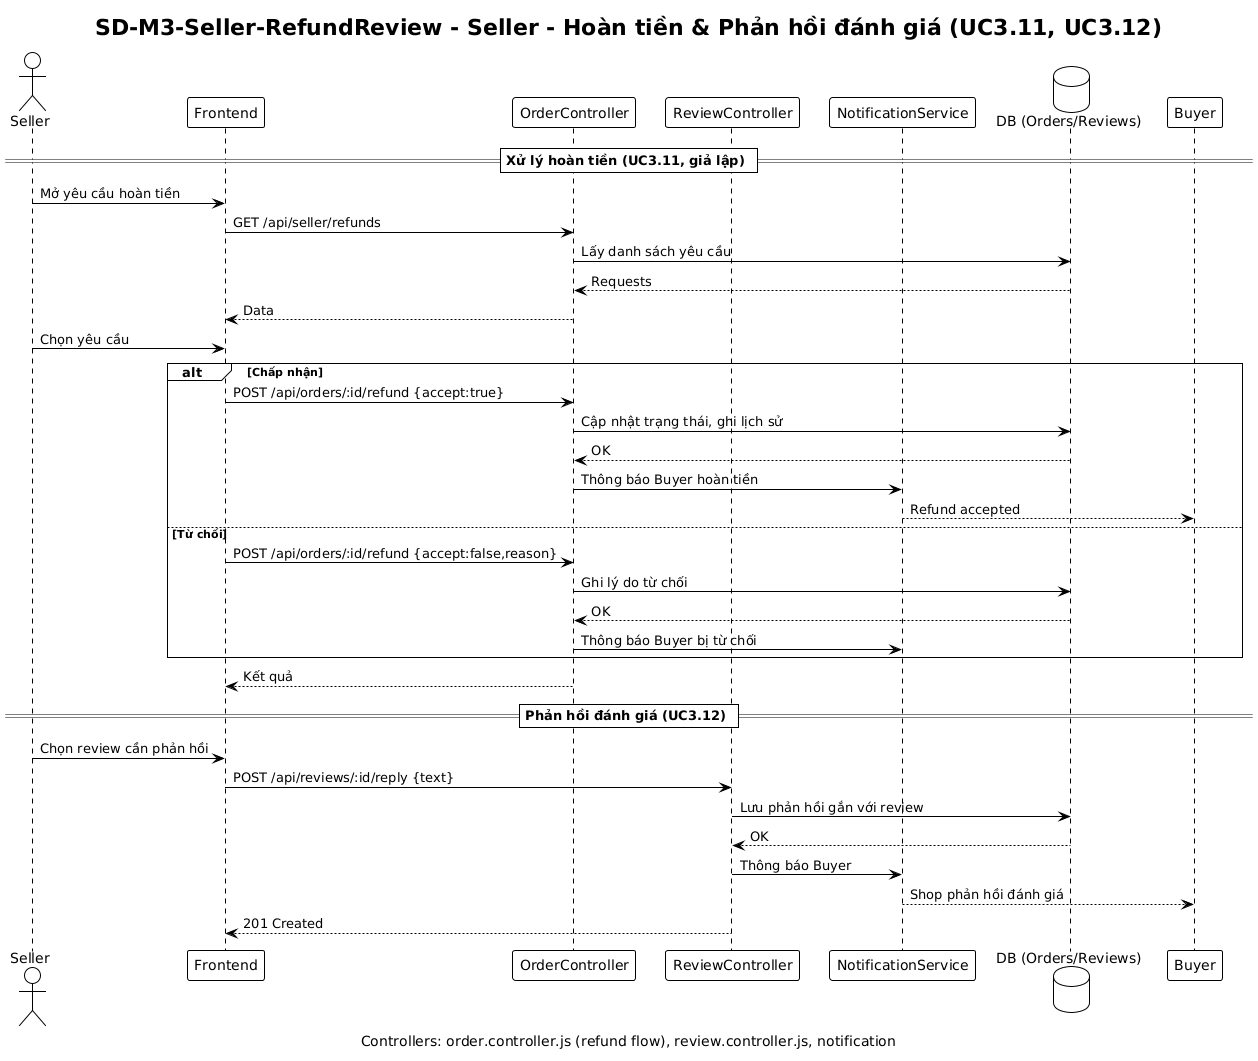
\includegraphics[width=\textwidth]{Images/Sequence diagrams/SD-M3-Seller-RefundReview.png}
  \caption{Sequence Diagram - Hoàn tiền và Phản hồi Đánh giá của Seller (SD-M3-Seller-RefundReview)}
\end{figure}

\subsection{Module 4 – Hệ thống Quản trị}

Module này mô tả luồng tương tác trong công cụ quản trị: quản lý tài khoản, quản lý nội dung, xử lý báo cáo vi phạm, và thống kê phân tích. Các diagram thể hiện cách Frontend giao tiếp với Admin Controllers (UsersController, PostsController, ProductsController, ReportsController, DashboardController) và Database.

\subsubsection{SD-M4-Admin-AccountsContent}

Diagram này mô tả chuỗi tương tác trong quá trình quản lý tài khoản và nội dung của Admin.

\textbf{UC4.1 – Quản lý tài khoản:} Admin Frontend gửi GET \texttt{/api/admin/users?filters=...} đến admin API với tham số lọc và admin JWT. AdminController xác thực token và vai trò Admin, truy vấn DB, trả về danh sách người dùng. Để thực hiện hành động: Frontend gửi PATCH \texttt{/api/admin/users/:id/toggle-active} hoặc PATCH \texttt{/api/admin/users/:id/role}. Controller xác thực quyền, cập nhật trong DB, trả về 200.

\textbf{UC4.2 – Quản lý nội dung:} Admin Frontend gửi GET \texttt{/api/admin/posts} hoặc \texttt{/api/admin/products} kèm admin JWT. AdminController xác thực token và vai trò Admin, truy vấn DB, trả về danh sách. Để xóa: Frontend gửi DELETE \texttt{/api/admin/posts/:id} hoặc \texttt{/api/admin/products/:id}. Controller xác thực quyền, xóa nội dung trong DB và trả về 200.

\begin{figure}[H]
  \centering
  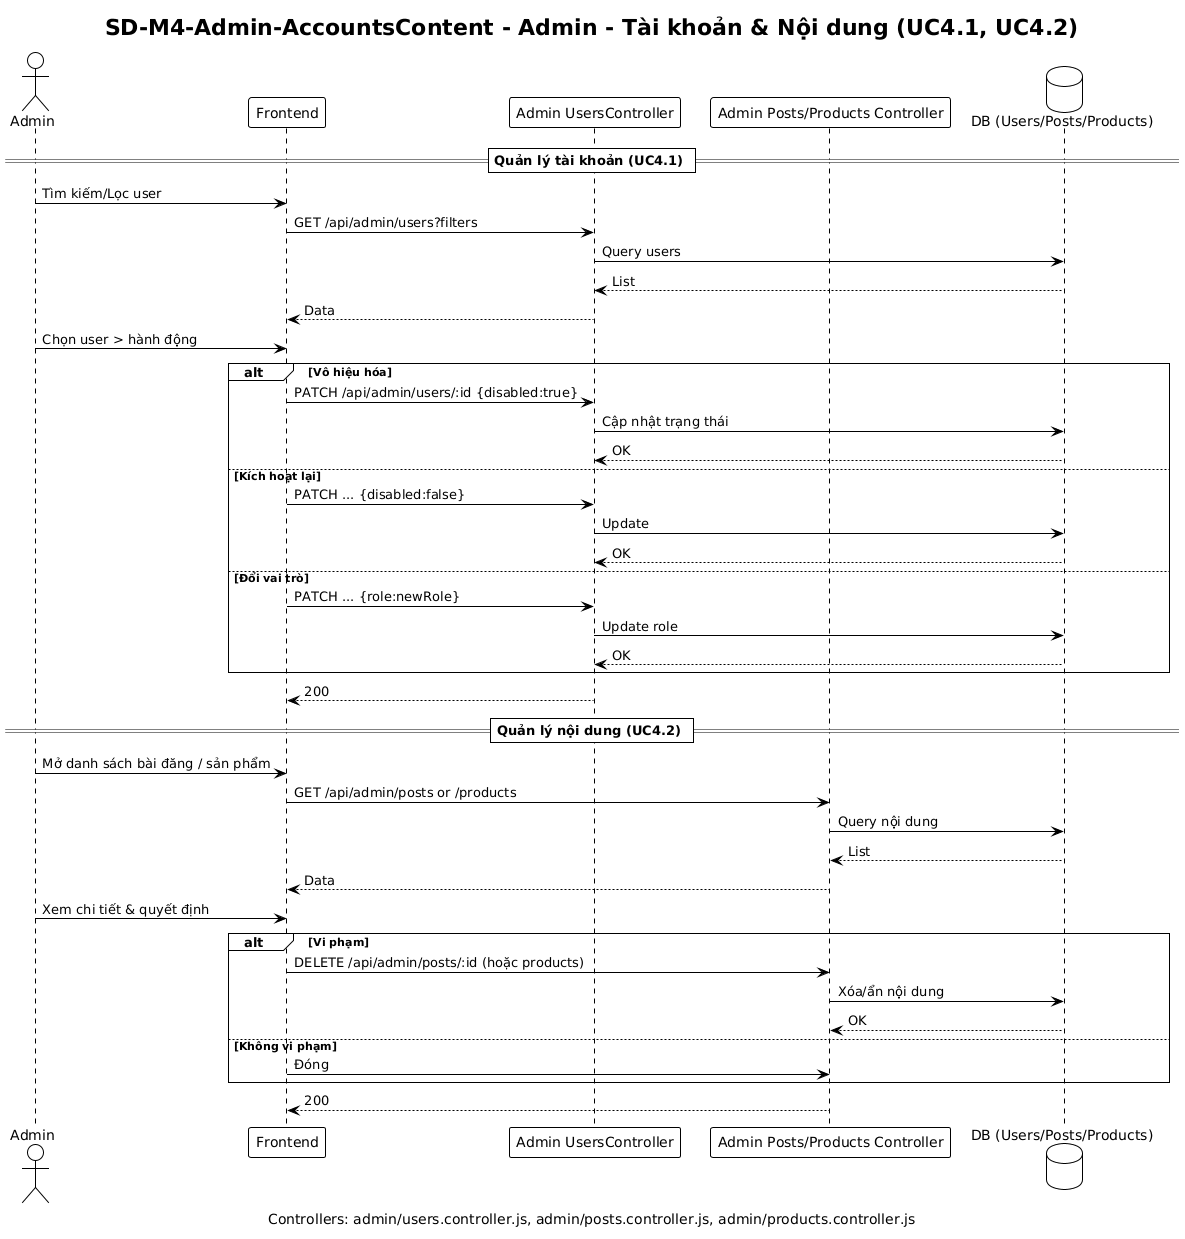
\includegraphics[width=\textwidth]{Images/Sequence diagrams/SD-M4-Admin-AccountsContent.png}
  \caption{Sequence Diagram - Quản lý Tài khoản và Nội dung của Admin (SD-M4-Admin-AccountsContent)}
\end{figure}

\subsubsection{SD-M4-Admin-ReportsAnalytics}

Diagram này mô tả chuỗi tương tác trong quá trình xử lý báo cáo và xem thống kê của Admin.

\textbf{UC4.3 – Xử lý báo cáo vi phạm:} Admin Frontend gửi GET \texttt{/api/reports?status=pending} đến admin API kèm admin JWT. ReportController xác thực, truy vấn DB lấy danh sách báo cáo pending, trả về danh sách. Để xem chi tiết: Frontend gửi GET \texttt{/api/reports/:reportId}. Để xử lý: Frontend gửi PATCH \texttt{/api/reports/:reportId/resolve} kèm action và admin JWT. Controller xác thực quyền, thực thi hành động trong DB, trả về 200.

\textbf{UC4.4 – Thống kê và phân tích:} Admin Frontend gửi GET \texttt{/api/admin/dashboard} hoặc \texttt{/api/admin/dashboard/growth?days=...} kèm admin JWT. AdminController xác thực, truy vấn DB tổng hợp số liệu về người dùng, bài đăng, sản phẩm, đơn hàng, doanh thu và growth, trả về dữ liệu thống kê.

\begin{figure}[H]
  \centering
  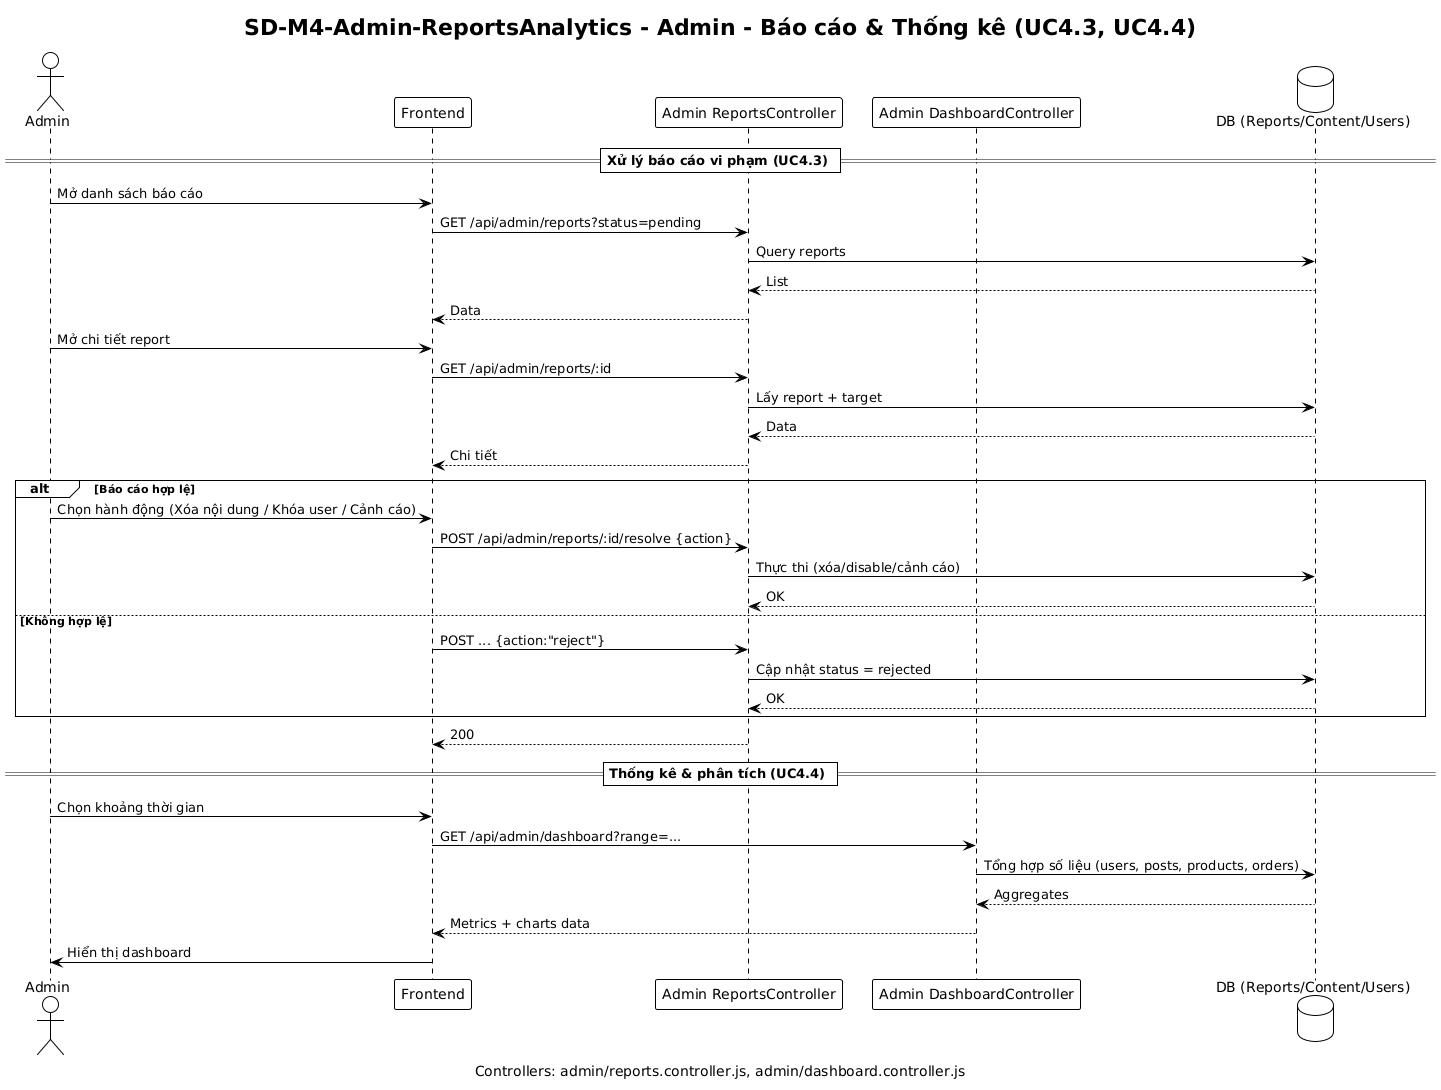
\includegraphics[width=\textwidth]{Images/Sequence diagrams/SD-M4-Admin-ReportsAnalytics.png}
  \caption{Sequence Diagram - Báo cáo và Thống kê của Admin (SD-M4-Admin-ReportsAnalytics)}
\end{figure}

\subsection{Module 5 – Tích hợp AI hỗ trợ}

Module này mô tả luồng tương tác trong tính năng AI hỗ trợ tạo nội dung và AI Shopping Assistant: generate text, generate image+text, quản lý lịch sử nội dung AI và chatbox tư vấn mua sắm. Các diagram thể hiện cách Frontend giao tiếp với AIController, AI Assistant Controller, AI Service, external AI providers và Database.

\subsubsection{SD-M5-AIContentCreation}

Diagram này mô tả chuỗi tương tác trong quá trình tạo nội dung sử dụng AI và tư vấn mua sắm qua chatbox.

\textbf{UC5.1 – Generate Text:} Frontend gửi POST \texttt{/api/ai/generate-text} kèm mô tả, ý tưởng, hình ảnh (nếu có) và JWT token. AIController xác thực, gọi AI Service. AI Service chuẩn hóa đầu vào, gọi text provider để sinh nội dung dạng cấu trúc, sau đó chạy bước đánh giá chất lượng (\textit{evaluate + score}). Nếu điểm chưa đạt ngưỡng, AI Service tự động \textit{refine prompt} và \textit{regenerate} theo vòng lặp giới hạn số lần thử. Nếu provider chính gặp lỗi quota/rate-limit, hệ thống retry/backoff và có thể chuyển sang provider dự phòng. Khi nội dung đạt ngưỡng, hệ thống lưu lịch sử và trả về văn bản với trạng thái chất lượng phù hợp.

\textbf{UC5.2 – Generate Image + Text:} Frontend gửi POST \texttt{/api/ai/generate-image-text} kèm mô tả, ý tưởng, hình ảnh đầu vào (nếu có) và JWT token. AIController xác thực và gọi AI Service. AI Service thực thi đầy đủ pipeline UC5.1 để bảo đảm chất lượng phần chữ, sau đó chuẩn hóa prompt ảnh (ưu tiên tiếng Anh) và gọi chuỗi image provider theo thứ tự chính/phụ. Nếu provider chính thất bại, hệ thống tự fallback sang provider kế tiếp. Nếu gặp lỗi quota/rate-limit hoặc toàn bộ provider ảnh không khả dụng, hệ thống \textit{degrade gracefully}: vẫn trả phần chữ đã đạt chuẩn cùng trạng thái lỗi ảnh để người dùng tiếp tục thao tác.

\textbf{UC5.3 – AI Shopping Assistant Chatbox:} Frontend gửi POST \texttt{/api/ai-assistant/chat} kèm câu hỏi, lịch sử hội thoại gần nhất, bộ nhớ phiên và JWT token. AiAssistantController xác thực người dùng, chuẩn hóa lịch sử, sau đó gọi AiAssistantService. Service phân tích intent, truy vấn dữ liệu sản phẩm/đơn hàng thuộc quyền truy cập của người dùng, gọi AI text provider để tạo phản hồi và trả về \texttt{reply}, \texttt{followUps}, \texttt{memory}, \texttt{cards} và \texttt{quickActions}. Frontend hiển thị phản hồi trong chatbox và thực hiện quick action như mở sản phẩm, thêm vào giỏ hàng hoặc xem chi tiết đơn hàng.

\begin{figure}[H]
  \centering
  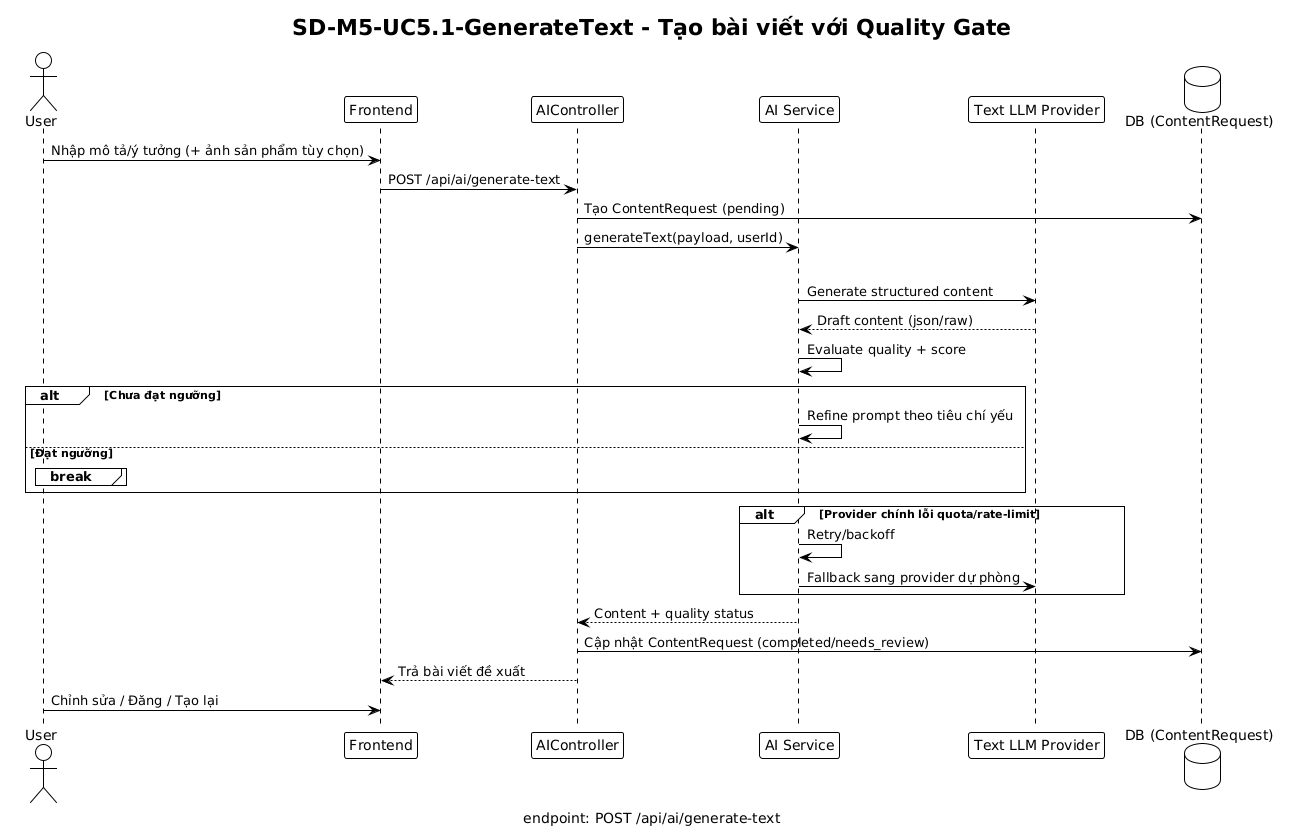
\includegraphics[width=\textwidth]{Images/Sequence diagrams/SD-M5-UC5.1-GenerateText.png}
  \caption{Sequence Diagram - Tạo bài viết với AI (SD-M5-UC5.1-GenerateText)}
\end{figure}

\begin{figure}[H]
  \centering
  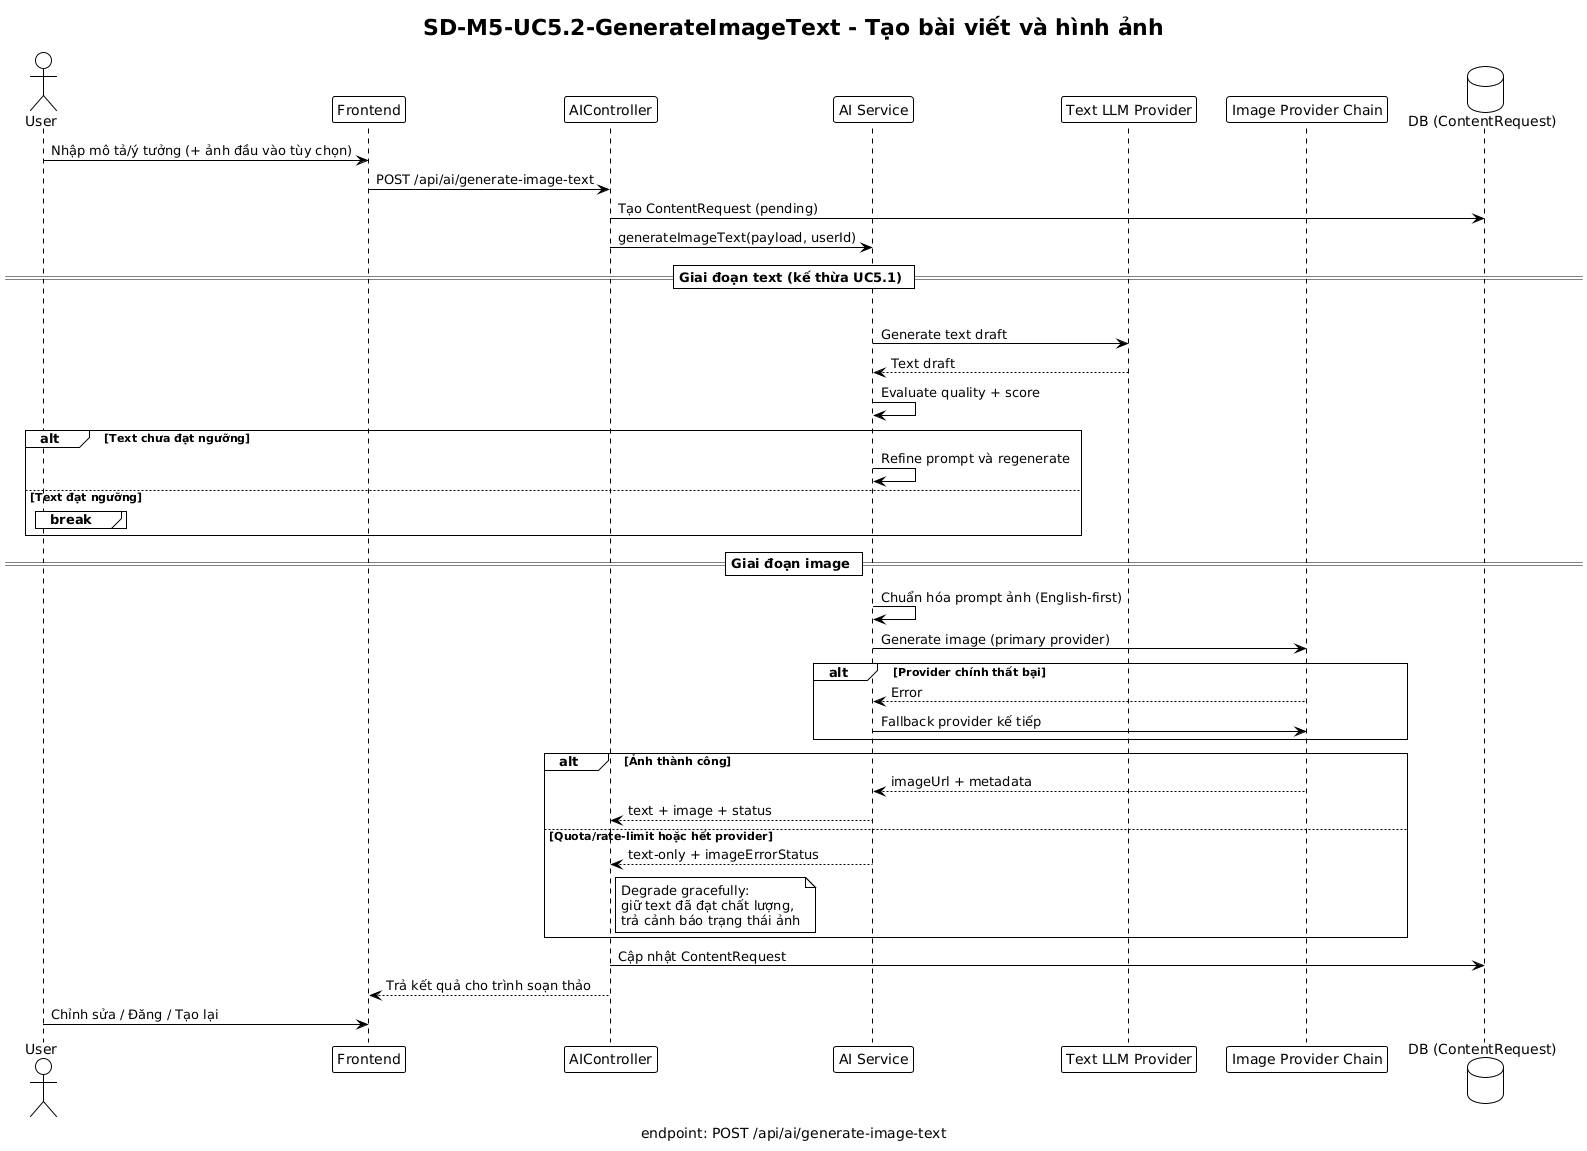
\includegraphics[width=\textwidth]{Images/Sequence diagrams/SD-M5-UC5.2-GenerateImageText.png}
  \caption{Sequence Diagram - Tạo bài viết và hình ảnh với AI (SD-M5-UC5.2-GenerateImageText)}
\end{figure}

\begin{figure}[H]
  \centering
  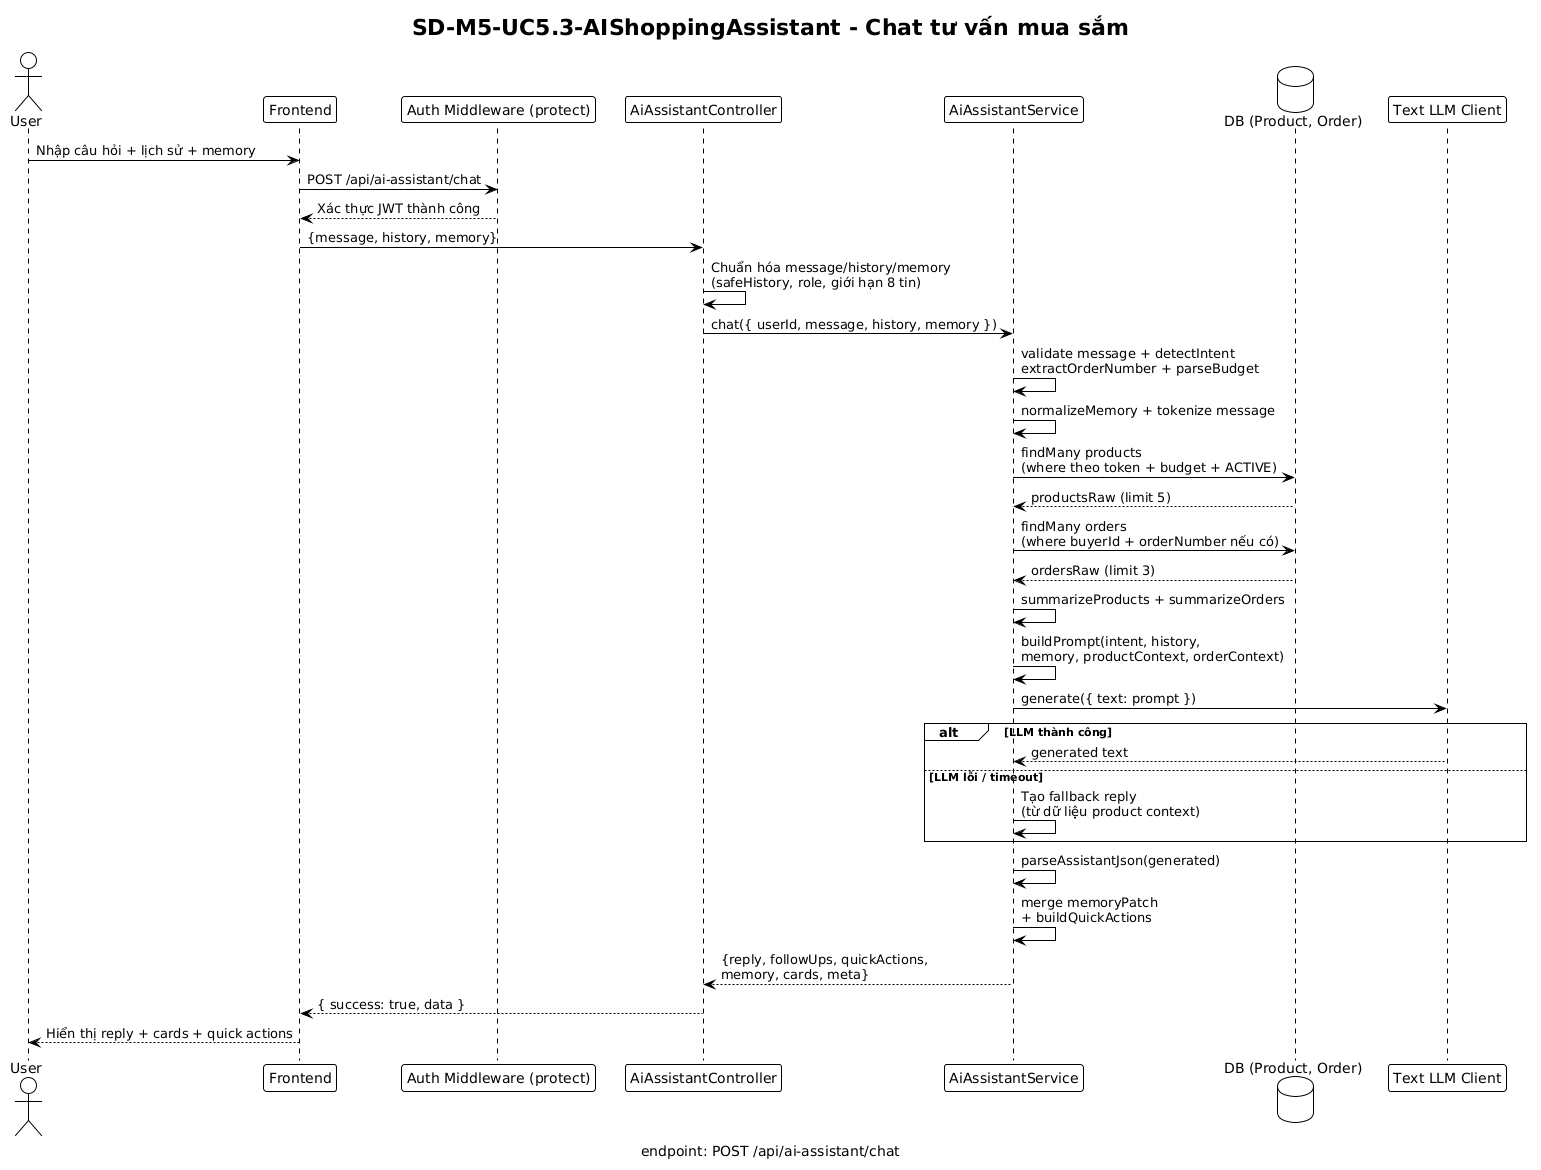
\includegraphics[width=\textwidth]{Images/Sequence diagrams/SD-M5-UC5.3-AIShoppingAssistant.png}
  \caption{Sequence Diagram - AI Shopping Assistant Chatbox (SD-M5-UC5.3-AIShoppingAssistant)}
\end{figure}

\subsection{Module 6 – Lên lịch và Điều phối Bài đăng}

Module này mô tả luồng tương tác trong tính năng lên lịch đăng bài: tạo lịch đăng, quản lý bài đăng đã lên lịch, và tự động xuất bản qua cron job. Các diagram thể hiện cách Frontend giao tiếp với PostController, Database và CronScheduler.

\subsubsection{SD-M6-PostScheduling}

Diagram này mô tả chuỗi tương tác trong quá trình lên lịch đăng bài và quản lý bài đăng đã lên lịch, bao gồm cả tác vụ tự động của cron job.

\textbf{UC6.1 – Lên lịch đăng bài:} Frontend gửi POST \texttt{/api/scheduled-posts} kèm nội dung, thời gian xuất bản (scheduledTime) và JWT token. ScheduledPostController xác thực, kiểm tra thời gian trong tương lai, lưu bài đăng với trạng thái \textit{scheduled} vào DB, trả về 201.

\textbf{UC6.2 – Quản lý bài đăng đã lên lịch:} Frontend gửi GET \texttt{/api/scheduled-posts} kèm JWT token. ScheduledPostController xác thực, truy vấn DB lấy danh sách bài đăng \textit{scheduled}, trả về danh sách. Để chỉnh sửa: Frontend gửi PUT \texttt{/api/scheduled-posts/:id}. Để đăng ngay: Frontend gửi POST \texttt{/api/scheduled-posts/:id/publish}. Để xóa: Frontend gửi DELETE \texttt{/api/scheduled-posts/:id}. Controller xử lý trong DB, trả về kết quả.

\textbf{Cron Job – Xuất bản tự động:} CronScheduler chạy định kỳ, truy vấn DB lấy scheduled posts có trạng thái \textit{scheduled} và thời gian đã đến. Scheduler tạo bản ghi Post tương ứng, cập nhật scheduled post thành \textit{published} và lưu publishedPostId.

\begin{figure}[H]
  \centering
  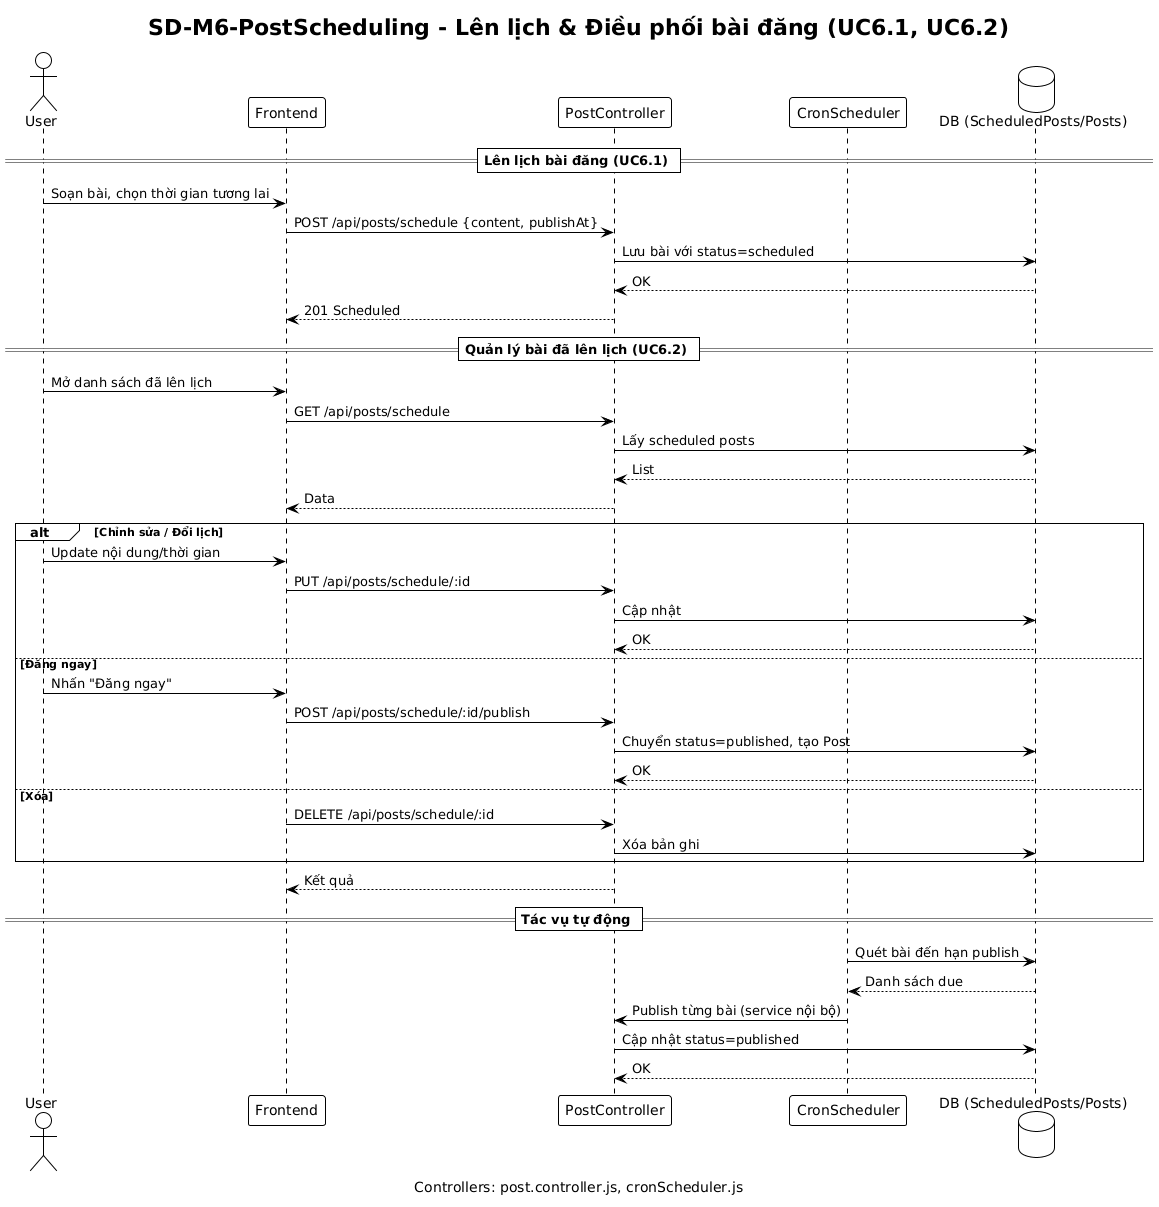
\includegraphics[width=\textwidth]{Images/Sequence diagrams/SD-M6-PostScheduling.png}
  \caption{Sequence Diagram - Lên lịch và Điều phối Bài đăng (SD-M6-PostScheduling)}
\end{figure}

\subsection{Module 7 – Hệ thống Thông báo}

Module này mô tả luồng tương tác trong hệ thống thông báo: tạo và gửi thông báo (tương tác xã hội, giao dịch), quản lý thông báo (xem, đánh dấu đã đọc, xóa), và cấu hình nhận thông báo. Các diagram thể hiện cách Frontend giao tiếp với NotificationController, NotificationService (Socket) và Database.

\subsubsection{SD-M7-NotificationSystem}

Diagram này mô tả chuỗi tương tác trong toàn bộ hệ thống thông báo, bao gồm bốn use case chính.

\textbf{UC7.1 – Thông báo tương tác:} Khi có sự kiện like, comment hoặc follow, service nghiệp vụ gọi NotificationService để tạo thông báo. NotificationService kiểm tra preference của người nhận, lưu thông báo vào DB và emit qua Socket.IO nếu người nhận online. Thông báo vẫn được lưu để hiển thị khi người nhận mở lại ứng dụng.

\textbf{UC7.2 – Thông báo giao dịch:} Khi có sự kiện giao dịch, hệ thống gọi NotificationController tạo thông báo. Controller lưu vào DB và gửi qua Socket đến Buyer/Seller. Nếu người nhận online và bật nhận, họ nhận real-time qua WebSocket.

\textbf{UC7.3 – Quản lý thông báo:} Frontend gửi GET \texttt{/api/notifications} kèm JWT token. NotificationController xác thực, truy vấn DB lấy danh sách thông báo (sắp xếp theo thời gian, mới nhất trước), trả về danh sách. Để đánh dấu đã đọc: Frontend gửi PATCH \texttt{/api/notifications/:id} với \texttt{\{read: true\}}. Để xóa: Frontend gửi DELETE \texttt{/api/notifications/:id}. Controller cập nhật/xóa trong DB, trả về 200.

\textbf{UC7.4 – Cài đặt thông báo:} Frontend gửi GET \texttt{/api/notifications/preferences} kèm JWT token. NotificationController xác thực, đọc cấu hình hiện tại từ privacySettings của user và trả về cấu hình. Để cập nhật: Frontend gửi PATCH \texttt{/api/notifications/preferences} kèm cấu hình mới và JWT token. Controller xác thực, lưu cấu hình vào DB, trả về 200. Cấu hình được áp dụng ngay lập tức.

\begin{figure}[H]
  \centering
  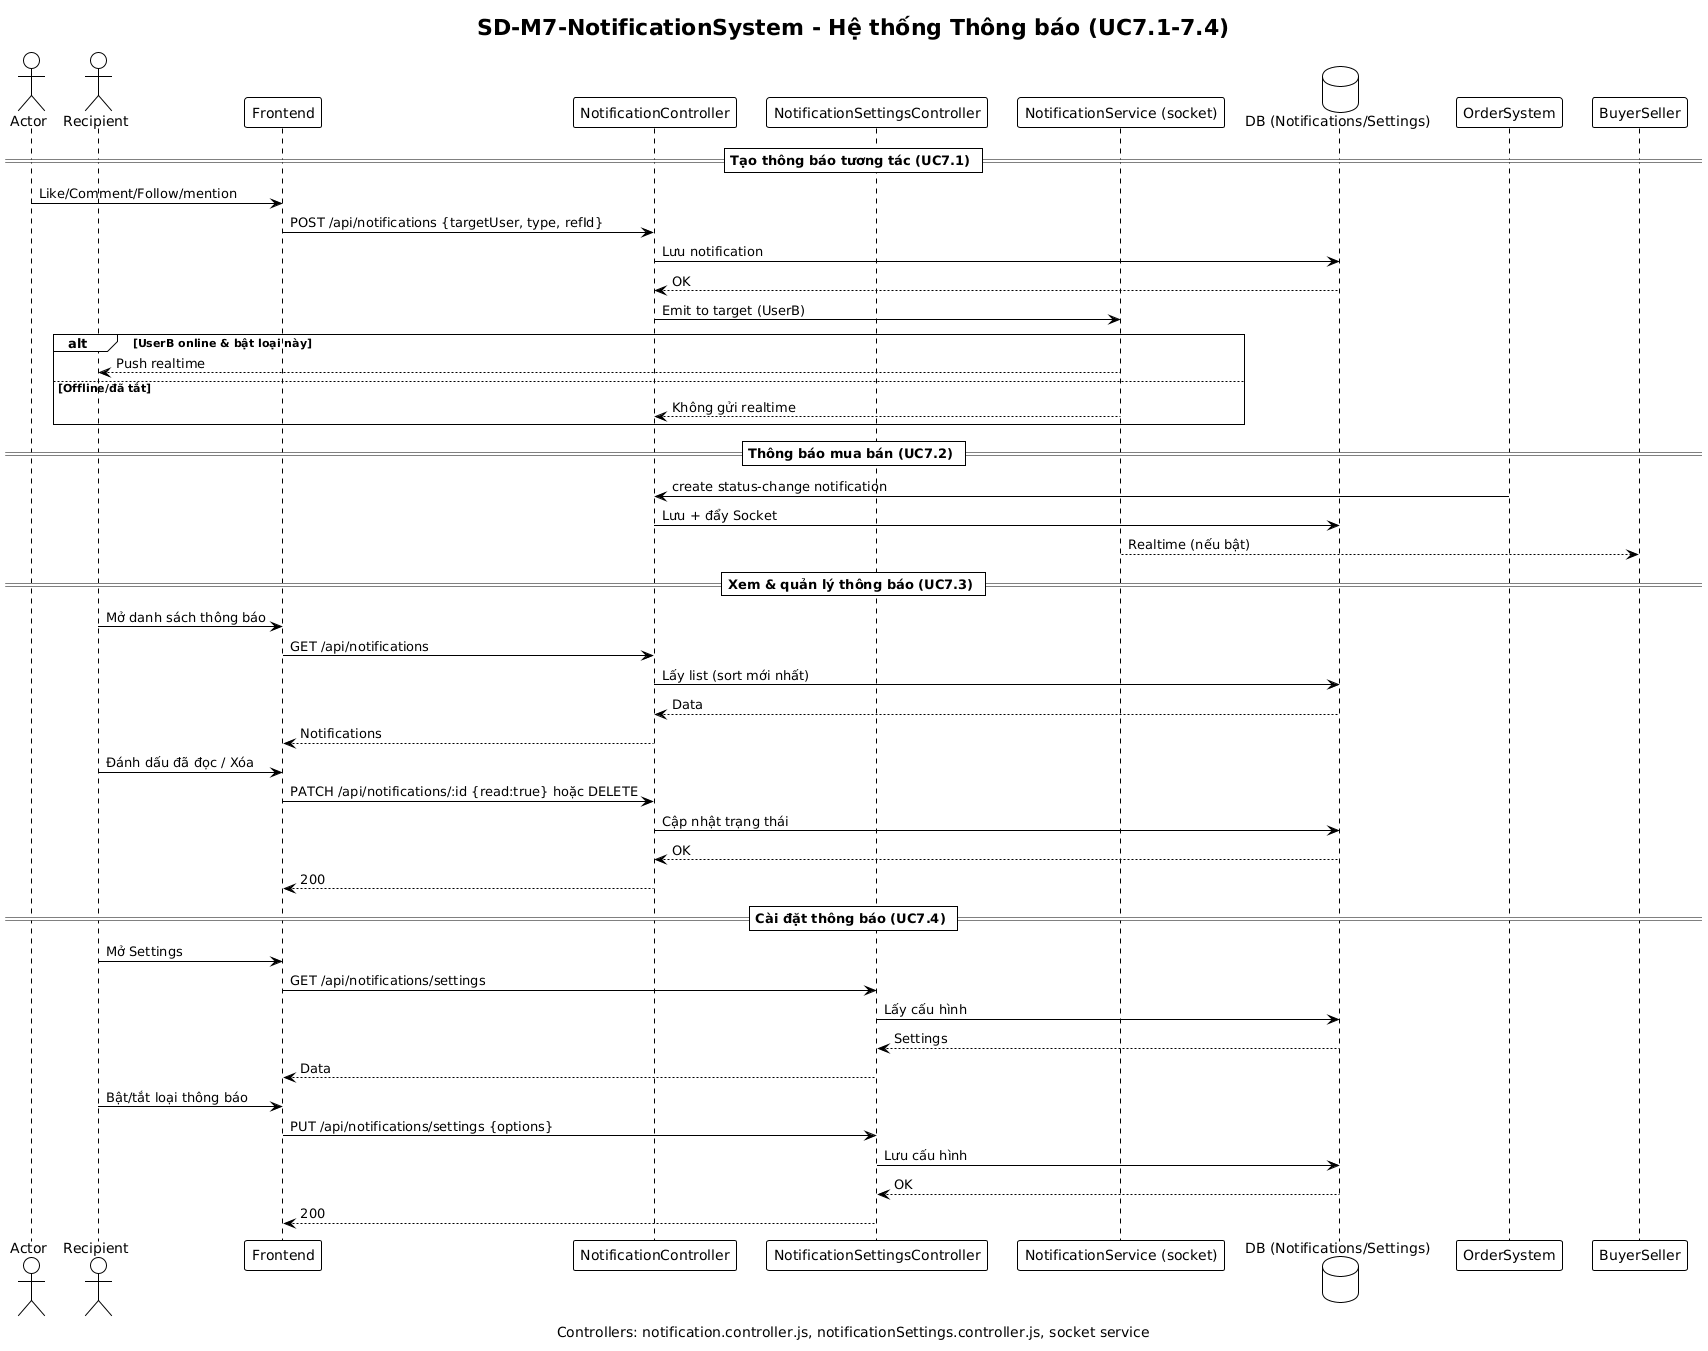
\includegraphics[width=\textwidth]{Images/Sequence diagrams/SD-M7-NotificationSystem.png}
  \caption{Sequence Diagram - Hệ thống Thông báo (SD-M7-NotificationSystem)}
\end{figure}


\section{Database design}
Dưới đây là mô tả chi tiết các entity, nêu ra vai trò, attribute và các relationship trong hệ thống.

\begin{figure}[H]
  \centering
  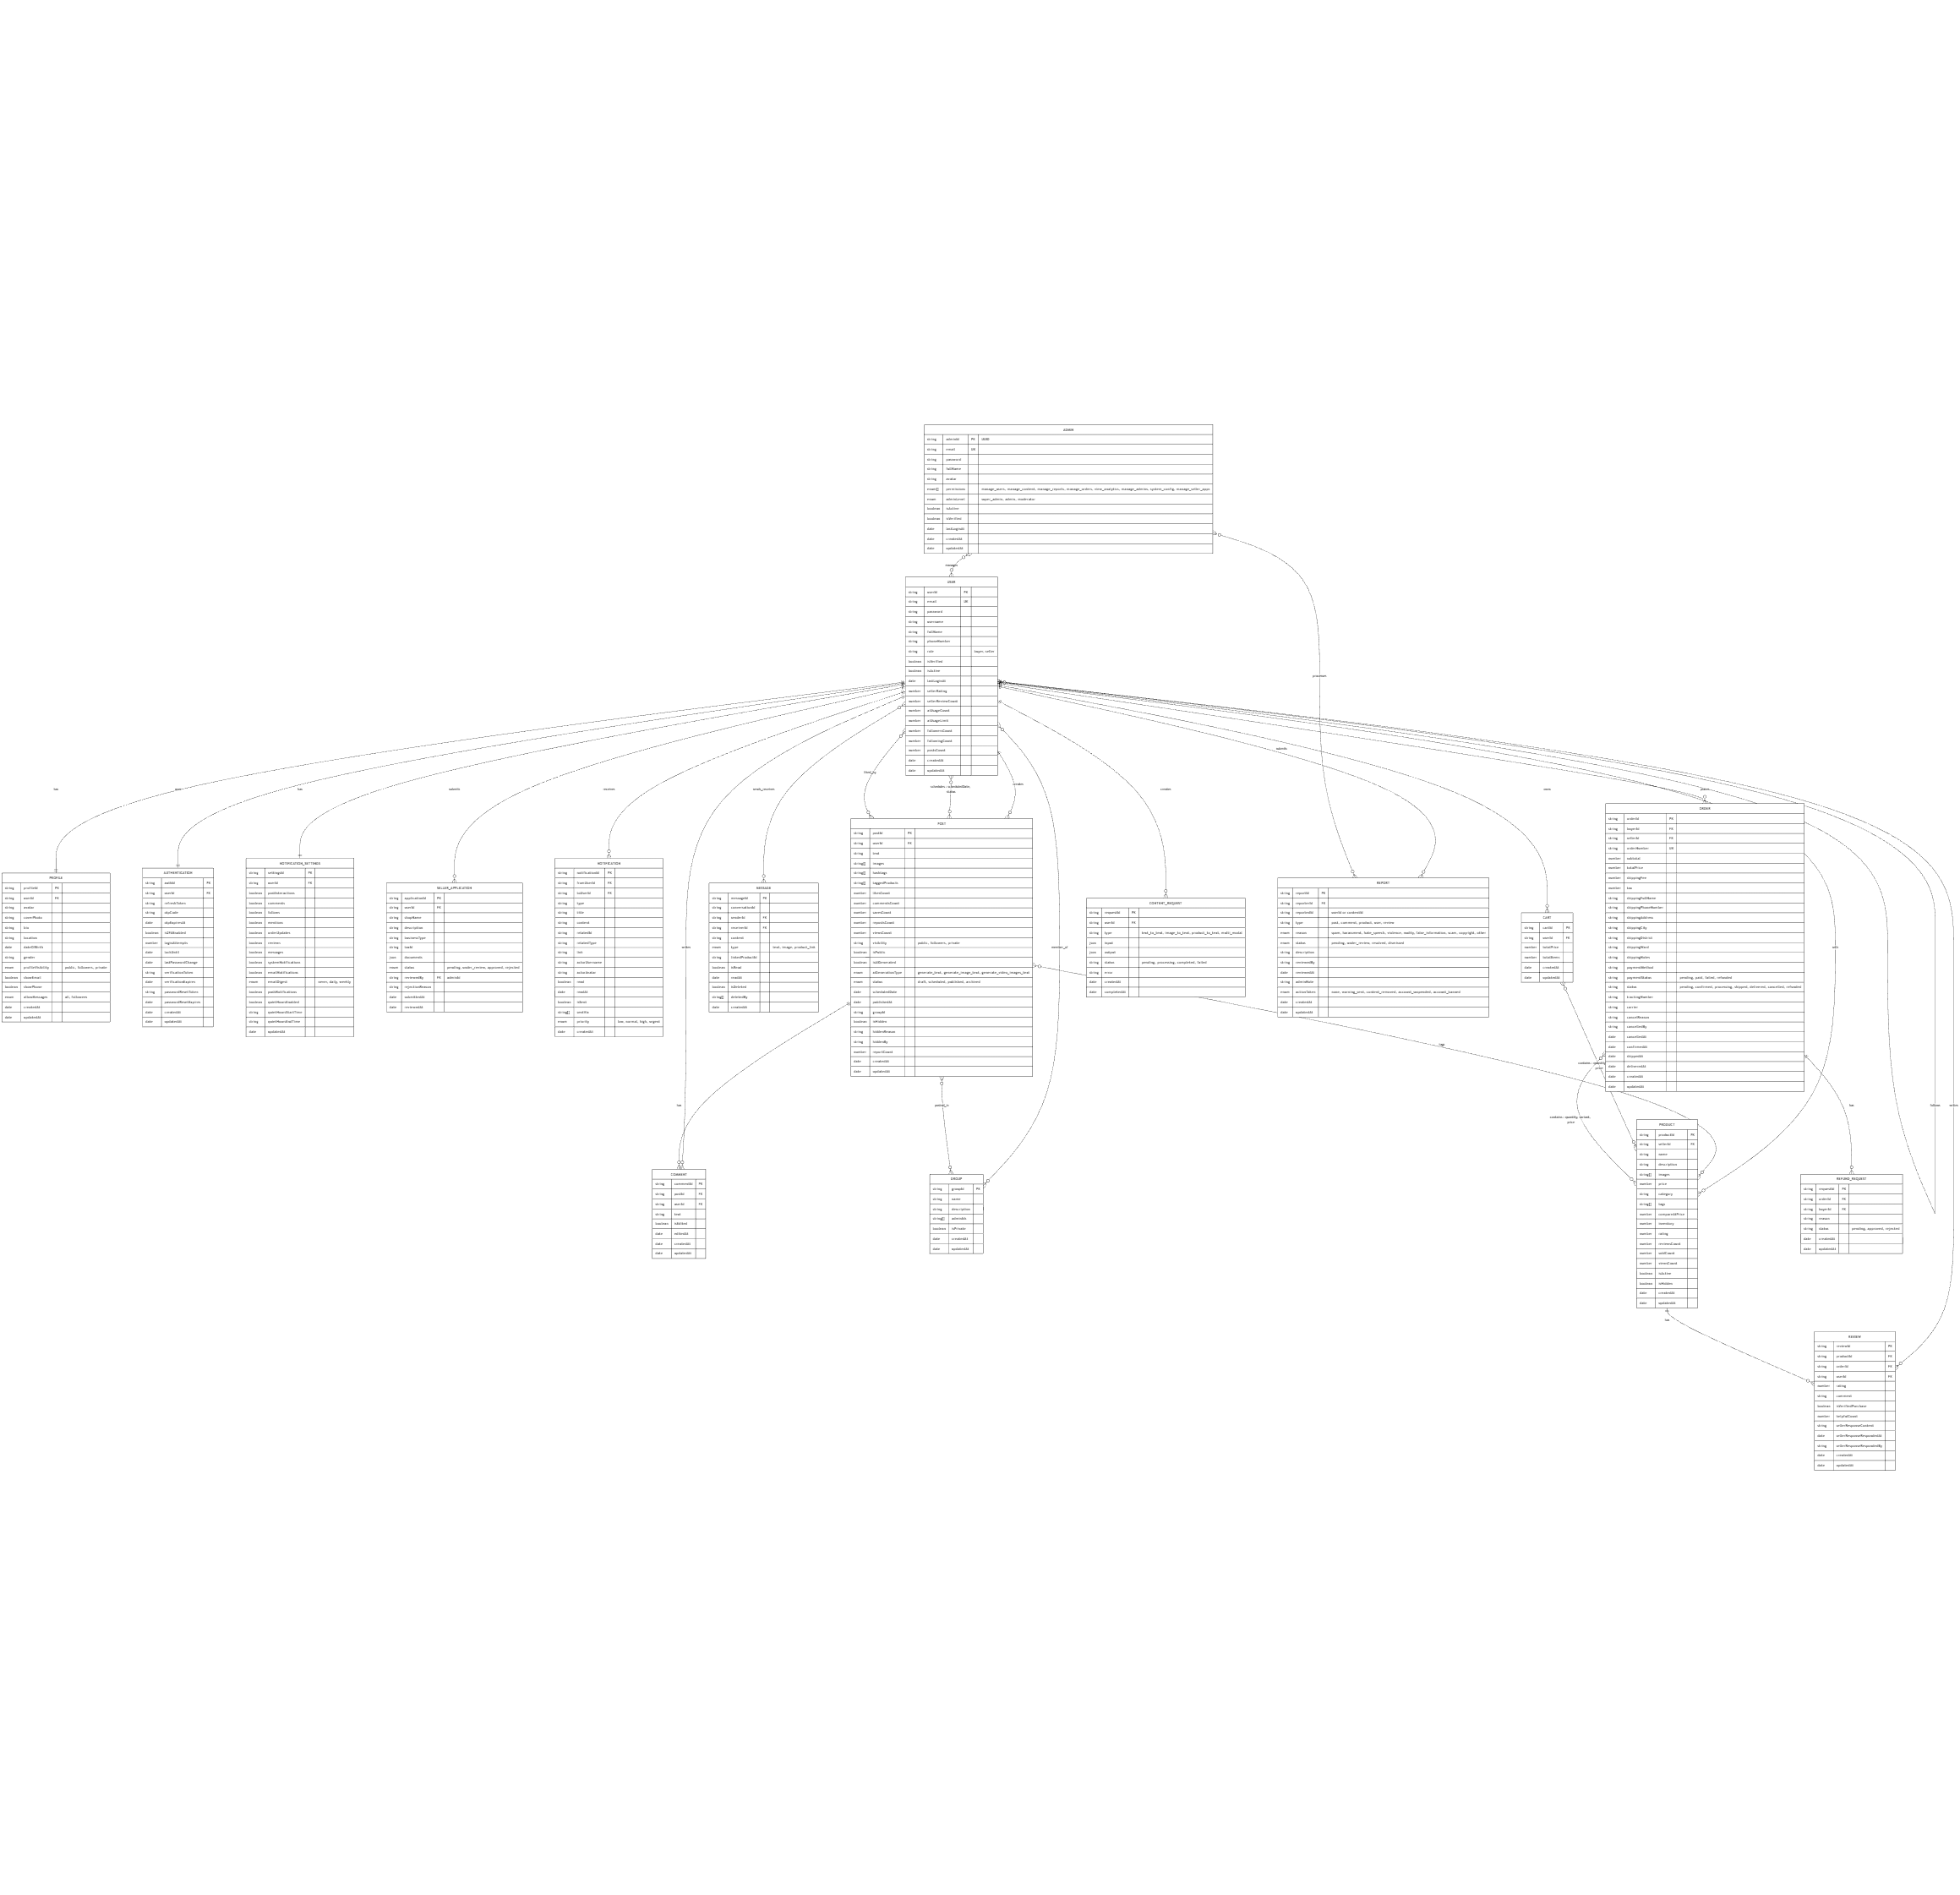
\includegraphics[width=\textwidth]{Images/ERD.png}
  \caption{Sơ đồ ERD (Entity Relationship Diagram) - Mô hình thực thể kết hợp của hệ thống}
  \label{fig:erd-diagram}
\end{figure}

\subsection{Thực thể (Entities)}
\paragraph{USER} Entity đại diện cho người dùng chung của hệ thống (buyer hoặc seller). Attributes: \textit{userId} (PK), email (UK), password, username, fullName, role (buyer/seller), isVerified, isActive, aiUsageCount (số lần đã sử dụng AI), aiUsageLimit (giới hạn số lần sử dụng AI), followersCount, followingCount, (...), createdAt, updatedAt.

\paragraph{PROFILE} Entity lưu trữ hồ sơ công khai/riêng tư gắn với người dùng. Attributes: \textit{profileId} (PK), \textit{userId} (FK), avatar, coverPhoto, bio, location, profileVisibility (public/followers/private), showEmail, allowMessages (all/followees), (...), createdAt, updatedAt.

\paragraph{AUTHENTICATION} Entity quản lý thông tin đăng nhập và bảo mật. Attributes: \textit{authId} (PK), \textit{userId} (FK), refreshToken, otpCode, otpExpiresAt, is2FAEnabled, loginAttempts, lockUntil, verificationToken, passwordResetToken, (...), createdAt, updatedAt.

\paragraph{NOTIFICATION\_SETTINGS} Entity lưu trữ cấu hình thông báo cá nhân. Attributes: \textit{settingsId} (PK), \textit{userId} (FK), postInteractions, comments, follows, orderUpdates, reviews, messages, emailNotifications, emailDigest (never/daily/weekly), pushNotifications, quietHoursEnabled, (...), updatedAt.

\paragraph{NOTIFICATION} Entity lưu trữ bản ghi thông báo gửi tới người dùng. Attributes: \textit{notificationId} (PK), fromUserId (FK), toUserId (FK), type, title, content, relatedId, relatedType, link, read, readAt, priority (low/normal/high/urgent), (...), createdAt.

\paragraph{POST} Entity đại diện cho bài viết của người dùng. Attributes: \textit{postId} (PK), \textit{userId} (FK), text (nội dung văn bản), images[] (danh sách ảnh), hashtags[], taggedProducts[], likesCount, commentsCount, viewsCount, visibility (public/followers/private), isAIGenerated (được tạo bởi AI), aiGenerationType (generate\_text/generate\_image\_text/generate\_video\_images\_text - loại tạo nội dung AI), status (draft/scheduled/published/archived), scheduledDate, publishedAt, (...), createdAt, updatedAt.

\paragraph{COMMENT} Entity đại diện cho bình luận trên bài viết. Attributes: \textit{commentId} (PK), \textit{postId} (FK), \textit{userId} (FK), text, isEdited, editedAt, createdAt, updatedAt.

\paragraph{GROUP} Entity đại diện cho nhóm cộng đồng. Attributes: \textit{groupId} (PK), name, description, adminIds[], isPrivate, createdAt, updatedAt.

\paragraph{MESSAGE} Entity lưu trữ tin nhắn giữa người dùng. Attributes: \textit{messageId} (PK), conversationId, senderId (FK), receiverId (FK), content, type (text/image/product\_link), linkedProductId, isRead, readAt, (...), createdAt.

\paragraph{PRODUCT} Entity đại diện cho sản phẩm do người bán đăng. Attributes: \textit{productId} (PK), sellerId (FK), name, description, images[], price, category, tags[], compareAtPrice, inventory, rating, reviewsCount, soldCount, viewsCount, isActive, (...), createdAt, updatedAt.

\paragraph{CART} Entity đại diện cho giỏ hàng của người mua. Attributes: \textit{cartId} (PK), \textit{userId} (FK), totalPrice, totalItems, createdAt, updatedAt.

\paragraph{ORDER} Entity đại diện cho đơn hàng giữa người mua và người bán. Attributes: \textit{orderId} (PK), buyerId (FK), sellerId (FK), orderNumber (UK), subtotal, totalPrice, shippingFee, shippingAddress, shippingCity, paymentMethod, paymentStatus (pending/paid/failed/refunded), status (pending/confirmed/processing/shipped/delivered/cancelled/refunded), trackingNumber, refund\_status, refund\_reason, (...), createdAt, updatedAt.

\paragraph{REVIEW} Entity đại diện cho đánh giá sản phẩm gắn với đơn. Attributes: \textit{reviewId} (PK), productId (FK), orderId (FK), userId (FK), rating, comment, isVerifiedPurchase, helpfulCount, sellerResponseContent, (...), createdAt, updatedAt.

\paragraph{REFUND\_REQUEST} Entity đại diện cho yêu cầu hoàn tiền cho đơn. \textbf{Lưu ý:} Trong schema thực tế, các trường refund được tích hợp vào bảng \textit{orders} (refund\_status, refund\_reason, refund\_requested\_at, refund\_processed\_at, refund\_processed\_by).

\paragraph{CONTENT\_REQUEST} Entity lưu trữ yêu cầu tạo nội dung AI. Attributes: \textit{requestId} (PK), userId (FK), type (generate\_text/generate\_image\_text/generate\_video\_images\_text - loại yêu cầu), input (json - dữ liệu đầu vào), output (json - kết quả đầu ra), status (pending/processing/completed/failed), error, createdAt, completedAt.

\paragraph{REPORT} Entity lưu trữ báo cáo vi phạm. Attributes: \textit{reportId} (PK), reporterId (FK), reportedId, type (post/comment/product/user/review), reason (spam/harassment/hate\_speech/violence/nudity/false\_information/scam/copyright/other), status (pending/under\_review/resolved/dismissed), description, reviewedBy, actionTaken (none/warning\_sent/content\_removed/account\_suspended/account\_banned), (...), createdAt, updatedAt.

\paragraph{SELLER\_APPLICATION} Entity lưu trữ hồ sơ đăng ký trở thành người bán. Attributes: \textit{applicationId} (PK), userId (FK), shopName, description, businessType, taxId, documents (json), status (pending/under\_review/approved/rejected), reviewedBy, rejectionReason, submittedAt, reviewedAt.

\paragraph{ADMIN} Entity đại diện cho tài khoản quản trị. Attributes: \textit{adminId} (PK, UUID), email (UK), password, fullName, avatar, permissions[] (manage\_users/manage\_content/manage\_reports/manage\_orders/view\_analytics/manage\_admins/system\_config/manage\_seller\_apps), adminLevel (super\_admin/admin/moderator), isActive, isVerified, lastLoginAt, createdAt, updatedAt.

\subsection{Mối quan hệ (Relationships)}
\begin{itemize}
  \item \textbf{USER -- PROFILE}: 1:1. Mỗi USER có đúng một PROFILE; mỗi PROFILE chỉ thuộc một USER.
  \item \textbf{USER -- AUTHENTICATION}: 1:1. Lưu token/OTP và cấu hình 2FA cho đúng một USER.
  \item \textbf{USER -- NOTIFICATION\_SETTINGS}: 1:1. Mỗi USER có cấu hình thông báo riêng.
  \item \textbf{USER -- NOTIFICATION}: 1:N. Một USER nhận nhiều thông báo qua toUserId; fromUserId ghi nhận tác nhân phát sinh.
  \item \textbf{USER -- SELLER\_APPLICATION}: 1:N. Người dùng có thể nộp nhiều đơn đăng ký bán.
  \item \textbf{ADMIN -- USER}: N:M (quản lý). ADMIN có thể quản lý nhiều USER và ngược lại (phân ca/phạm vi).
  \item \textbf{USER -- USER (follow)}: N:M. Người dùng có thể theo dõi lẫn nhau.
  \item \textbf{POST -- COMMENT}: 1:N. Một POST có nhiều COMMENT; COMMENT thuộc duy nhất một POST.
  \item \textbf{USER -- POST}: 1:N. Người dùng tạo nhiều POST; mỗi POST thuộc một USER.
  \item \textbf{USER -- COMMENT}: 1:N. Người dùng viết nhiều COMMENT.
  \item \textbf{POST -- USER (liked\_by)}: N:M. Một bài có nhiều người thích; một người thích nhiều bài.
  \item \textbf{POST -- GROUP (posted\_in)}: N:M. Bài viết có thể được đăng trong nhiều GROUP; GROUP chứa nhiều bài.
  \item \textbf{POST -- PRODUCT (tags)}: N:M. Bài viết có thể gắn nhiều sản phẩm; sản phẩm có thể được tag ở nhiều bài.
  \item \textbf{USER -- GROUP (member\_of)}: N:M. Người dùng có thể tham gia nhiều nhóm; nhóm có nhiều thành viên.
  \item \textbf{USER -- MESSAGE}: N:M. Một USER gửi/nhận nhiều MESSAGE; mỗi MESSAGE có sender và receiver.
  \item \textbf{USER -- POST (schedules)}: N:M qua thuộc tính scheduling. Một USER có thể lên lịch nhiều POST; một POST có thể có bản ghi lịch.
  \item \textbf{USER -- PRODUCT}: 1:N. Một người bán đăng nhiều PRODUCT; mỗi PRODUCT thuộc một seller.
  \item \textbf{CART -- PRODUCT}: N:M. Một CART chứa nhiều PRODUCT (kèm quantity/variant/price trên dòng giỏ); một PRODUCT có thể nằm trong nhiều CART.
  \item \textbf{ORDER -- PRODUCT}: N:M. Một ORDER chứa nhiều PRODUCT (dòng hàng gồm quantity/variant/price); một PRODUCT xuất hiện trong nhiều ORDER.
  \item \textbf{USER -- CART}: 1:N (thiết kế cho phép nhiều giỏ theo phiên; thực tế thường 1). Mỗi CART thuộc một USER.
  \item \textbf{USER -- ORDER}: 1:N. Người mua có nhiều ORDER; mỗi ORDER gắn với một buyer. Đồng thời ORDER giữ sellerId để biết người bán.
  \item \textbf{USER -- REVIEW}: 1:N. Người dùng viết nhiều REVIEW.
  \item \textbf{PRODUCT -- REVIEW}: 1:N. Một PRODUCT có nhiều REVIEW.
  \item \textbf{ORDER -- REFUND\_REQUEST}: 1:N. Một ORDER có thể phát sinh nhiều REFUND\_REQUEST.
  \item \textbf{USER -- REFUND\_REQUEST}: 1:N. Người mua gửi nhiều yêu cầu hoàn.
  \item \textbf{USER -- CONTENT\_REQUEST}: 1:N. Người dùng tạo nhiều yêu cầu AI; mỗi yêu cầu thuộc một USER.
  \item \textbf{USER -- REPORT}: 1:N. Người dùng có thể gửi nhiều REPORT; mỗi REPORT có một reporter.
  \item \textbf{ADMIN -- REPORT}: N:M. Nhiều ADMIN có thể xử lý các REPORT, mỗi REPORT có thể được giao/lưu vết nhiều admin.
\end{itemize}

\subsection{Chuyển đổi từ ERD sang Database Schema}

Quá trình chuyển đổi từ mô hình ERD sang database schema PostgreSQL đã được thực hiện với các quyết định thiết kế cụ thể để tối ưu performance, đảm bảo data integrity và hỗ trợ các tính năng của hệ thống.

\subsubsection{Quyết định về cấu trúc bảng (Table Structure)}

\paragraph{Junction Tables cho quan hệ N:M}
Để hỗ trợ các relationship N:M, hệ thống đã tách thành các junction table riêng biệt thay vì sử dụng array:

\begin{itemize}
  \item \textbf{post\_likes}: Lưu trữ relationship giữa POST và USER (liked\_by). Mỗi record gồm post\_id, user\_id và created\_at. Có UNIQUE constraint (post\_id, user\_id) để đảm bảo một người dùng chỉ like một bài viết một lần.
  \item \textbf{post\_saves}: Tương tự cho chức năng lưu bài viết (bookmark).
  \item \textbf{post\_reposts}: Lưu trữ các bài viết được chia sẻ lại (repost).
  \item \textbf{review\_helpful\_votes}: Lưu trữ các vote "hữu ích" cho đánh giá sản phẩm.
  \item \textbf{group\_members}: Quản lý thành viên của nhóm với role (member/admin/moderator), thay vì chỉ dùng adminIds[] trong GROUP.
  \item \textbf{user\_follows}: Relationship follow giữa người dùng với UNIQUE constraint (follower\_id, following\_id) và CHECK constraint để tránh tự follow.
  \item \textbf{user\_blocks}: Relationship block giữa người dùng (không có trong ERD nhưng cần thiết cho tính năng chặn người dùng).
\end{itemize}

\paragraph{Denormalization}
Một số quyết định gộp bảng để tối ưu query performance:

\begin{itemize}
  \item \textbf{REFUND\_REQUEST → orders}: Thay vì tạo bảng REFUND\_REQUEST riêng như trong ERD, các trường refund được tích hợp trực tiếp vào bảng \textit{orders}:
  \begin{itemize}
    \item refund\_requested (BOOLEAN)
    \item refund\_status (pending/approved/rejected)
    \item refund\_reason (TEXT)
    \item refund\_requested\_at, refund\_processed\_at (TIMESTAMP)
    \item refund\_processed\_by (FK → users)
  \end{itemize}
  Lý do: Mỗi đơn hàng chỉ có tối đa một yêu cầu hoàn tiền, việc gộp giảm số lượng JOIN và tăng query performance.
\end{itemize}

\paragraph{Supporting Tables}
Các bảng hỗ trợ được tách để quản lý metadata và lịch sử:

\begin{itemize}
  \item \textbf{product\_images}: Tách từ images[] trong PRODUCT để lưu metadata (url, public\_id, is\_primary, width, height) và hỗ trợ quản lý ảnh tốt hơn.
  \item \textbf{post\_images}: Tương tự cho POST (mặc dù posts vẫn giữ images[] để backward compatibility).
  \item \textbf{review\_images}: Ảnh đính kèm trong đánh giá sản phẩm.
  \item \textbf{report\_screenshots}: Ảnh chụp màn hình trong báo cáo vi phạm.
  \item \textbf{order\_status\_history}: Lưu lịch sử thay đổi trạng thái đơn hàng với timestamp, note và updated\_by để audit trail.
  \item \textbf{product\_variants} và \textbf{product\_variant\_options}: Hỗ trợ biến thể sản phẩm (size, color, etc.) với giá và tồn kho riêng.
\end{itemize}

\subsubsection{Sơ đồ Relational Mapping}
Hình \ref{fig:relational-mapping} mô tả sơ đồ relational mapping của hệ thống, thể hiện tất cả các bảng và mối quan hệ giữa chúng thông qua Primary Keys (PK) và Foreign Keys (FK). Sơ đồ này được tạo từ database schema PostgreSQL thực tế, bao gồm các junction tables cho quan hệ N:M và các supporting tables đã được mô tả ở trên.

\begin{figure}[H]
  \centering
  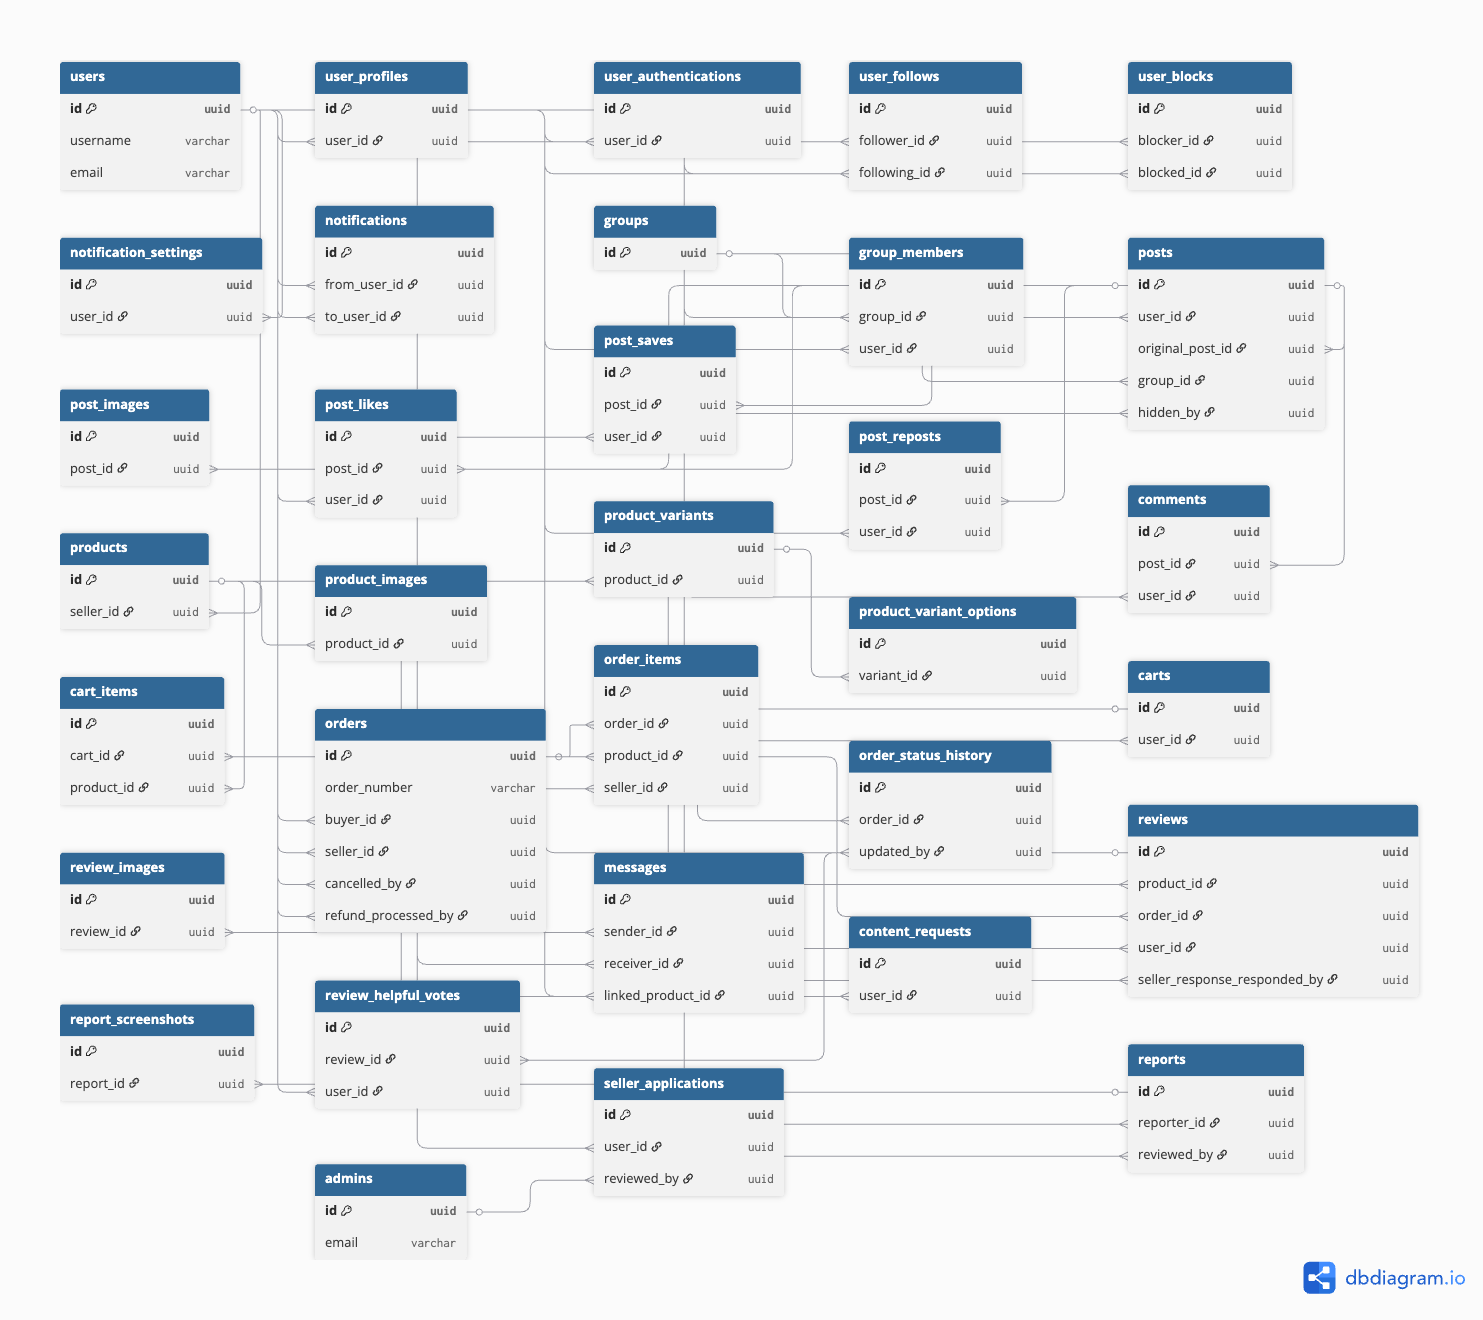
\includegraphics[width=\textwidth]{Images/Relation-Mapping.png}
  \caption{Sơ đồ Relational Mapping - Các bảng và mối quan hệ trong database schema}
  \label{fig:relational-mapping}
\end{figure}


\section{Architecture design}
\subsection{Architectural pattern}

Dự án sử dụng mô hình \textbf{MVCS}. Kiến trúc chuẩn của \textbf{MVCS} được thể hiện trong \ref{fig:mvcs-pattern}:

\begin{figure}[htbp]
    \centering
    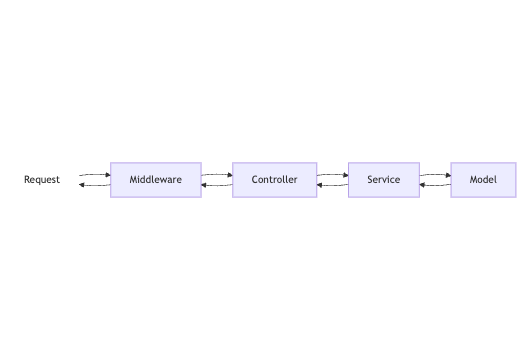
\includegraphics[width=0.8\textwidth]{Images/MVCS.png}
    \caption{MVCS pattern}
    \label{fig:mvcs-pattern}
\end{figure}

\textbf{MVCS} là viết tắt của \textbf{Model-View-Controller-Service}. Mô hình này cho phép lập trình viên định nghĩa trước sự tương tác giữa các phần code và dễ dàng chỉnh sửa bằng cách chia code thành các \textbf{layer} theo chức năng. Kiến trúc này không thuộc về bất kỳ ngôn ngữ lập trình hay framework cụ thể nào. \textbf{Pattern} này tách biệt \textbf{Database} hoặc \textbf{networking interaction} khỏi \textbf{Controller}. Mỗi phần đóng vai trò quan trọng trong việc phát triển ứng dụng.

\begin{itemize}
    \item \textbf{View Layer}: Đại diện cho cách dữ liệu được render lên giao diện người dùng. Trong dự án này, \textbf{View Layer} được xây dựng bằng \textbf{React.js} với các \textbf{Router} quản lý navigation và các \textbf{Component} hiển thị dữ liệu.
    \item \textbf{Controller Layer}: Chịu trách nhiệm chỉ nhận \textbf{request} và hiển thị kết quả của thao tác. \textbf{Controller} được sử dụng để giao tiếp giữa \textbf{Model}, \textbf{Service} và \textbf{View}. Trong \textbf{Backend Node.js}, các \textbf{Controller} như \textbf{Auth Controller}, \textbf{User Controller}, \textbf{Post Controller} xử lý các request từ \textbf{Frontend} và trả về \textbf{response} tương ứng.
    \item \textbf{Service Layer}: Còn được gọi là \textbf{Business Layer}, chứa các chức năng tạo nên core của ứng dụng, do đó trở nên \textbf{highly reusable} cho controllers và services. \textbf{Service Layer} xử lý \textbf{business logic} phức tạp, tách biệt khỏi \textbf{Controller} để dễ dàng maintain và test.
    \item \textbf{Model Layer}: Chịu trách nhiệm định nghĩa cách \textbf{data model} được định nghĩa. \textbf{Model Layer} sử dụng \textbf{Sequelize ORM} để ánh xạ các \textbf{entity} trong database như \textbf{User}, \textbf{Post}, \textbf{Product}, \textbf{Order}, \textbf{Message} và \textbf{Notification}.
\end{itemize}

\subsection{Architecture diagram}

\ref{fig:architecture-diagram} minh họa tổng quan cách chúng tôi lên kế hoạch triển khai hệ thống. Đối với \textbf{frontend}, tất cả các thiết kế đã được thực hiện với \textbf{Figma} sẽ được implement bằng \textbf{React.js} và cấu trúc được tổ chức như trong hình. \textbf{Frontend} được kết nối với \textbf{Backend Node.js} thông qua \textbf{HTTP request} và \textbf{WebSocket connection}.

\begin{figure}[htbp]
    \centering
    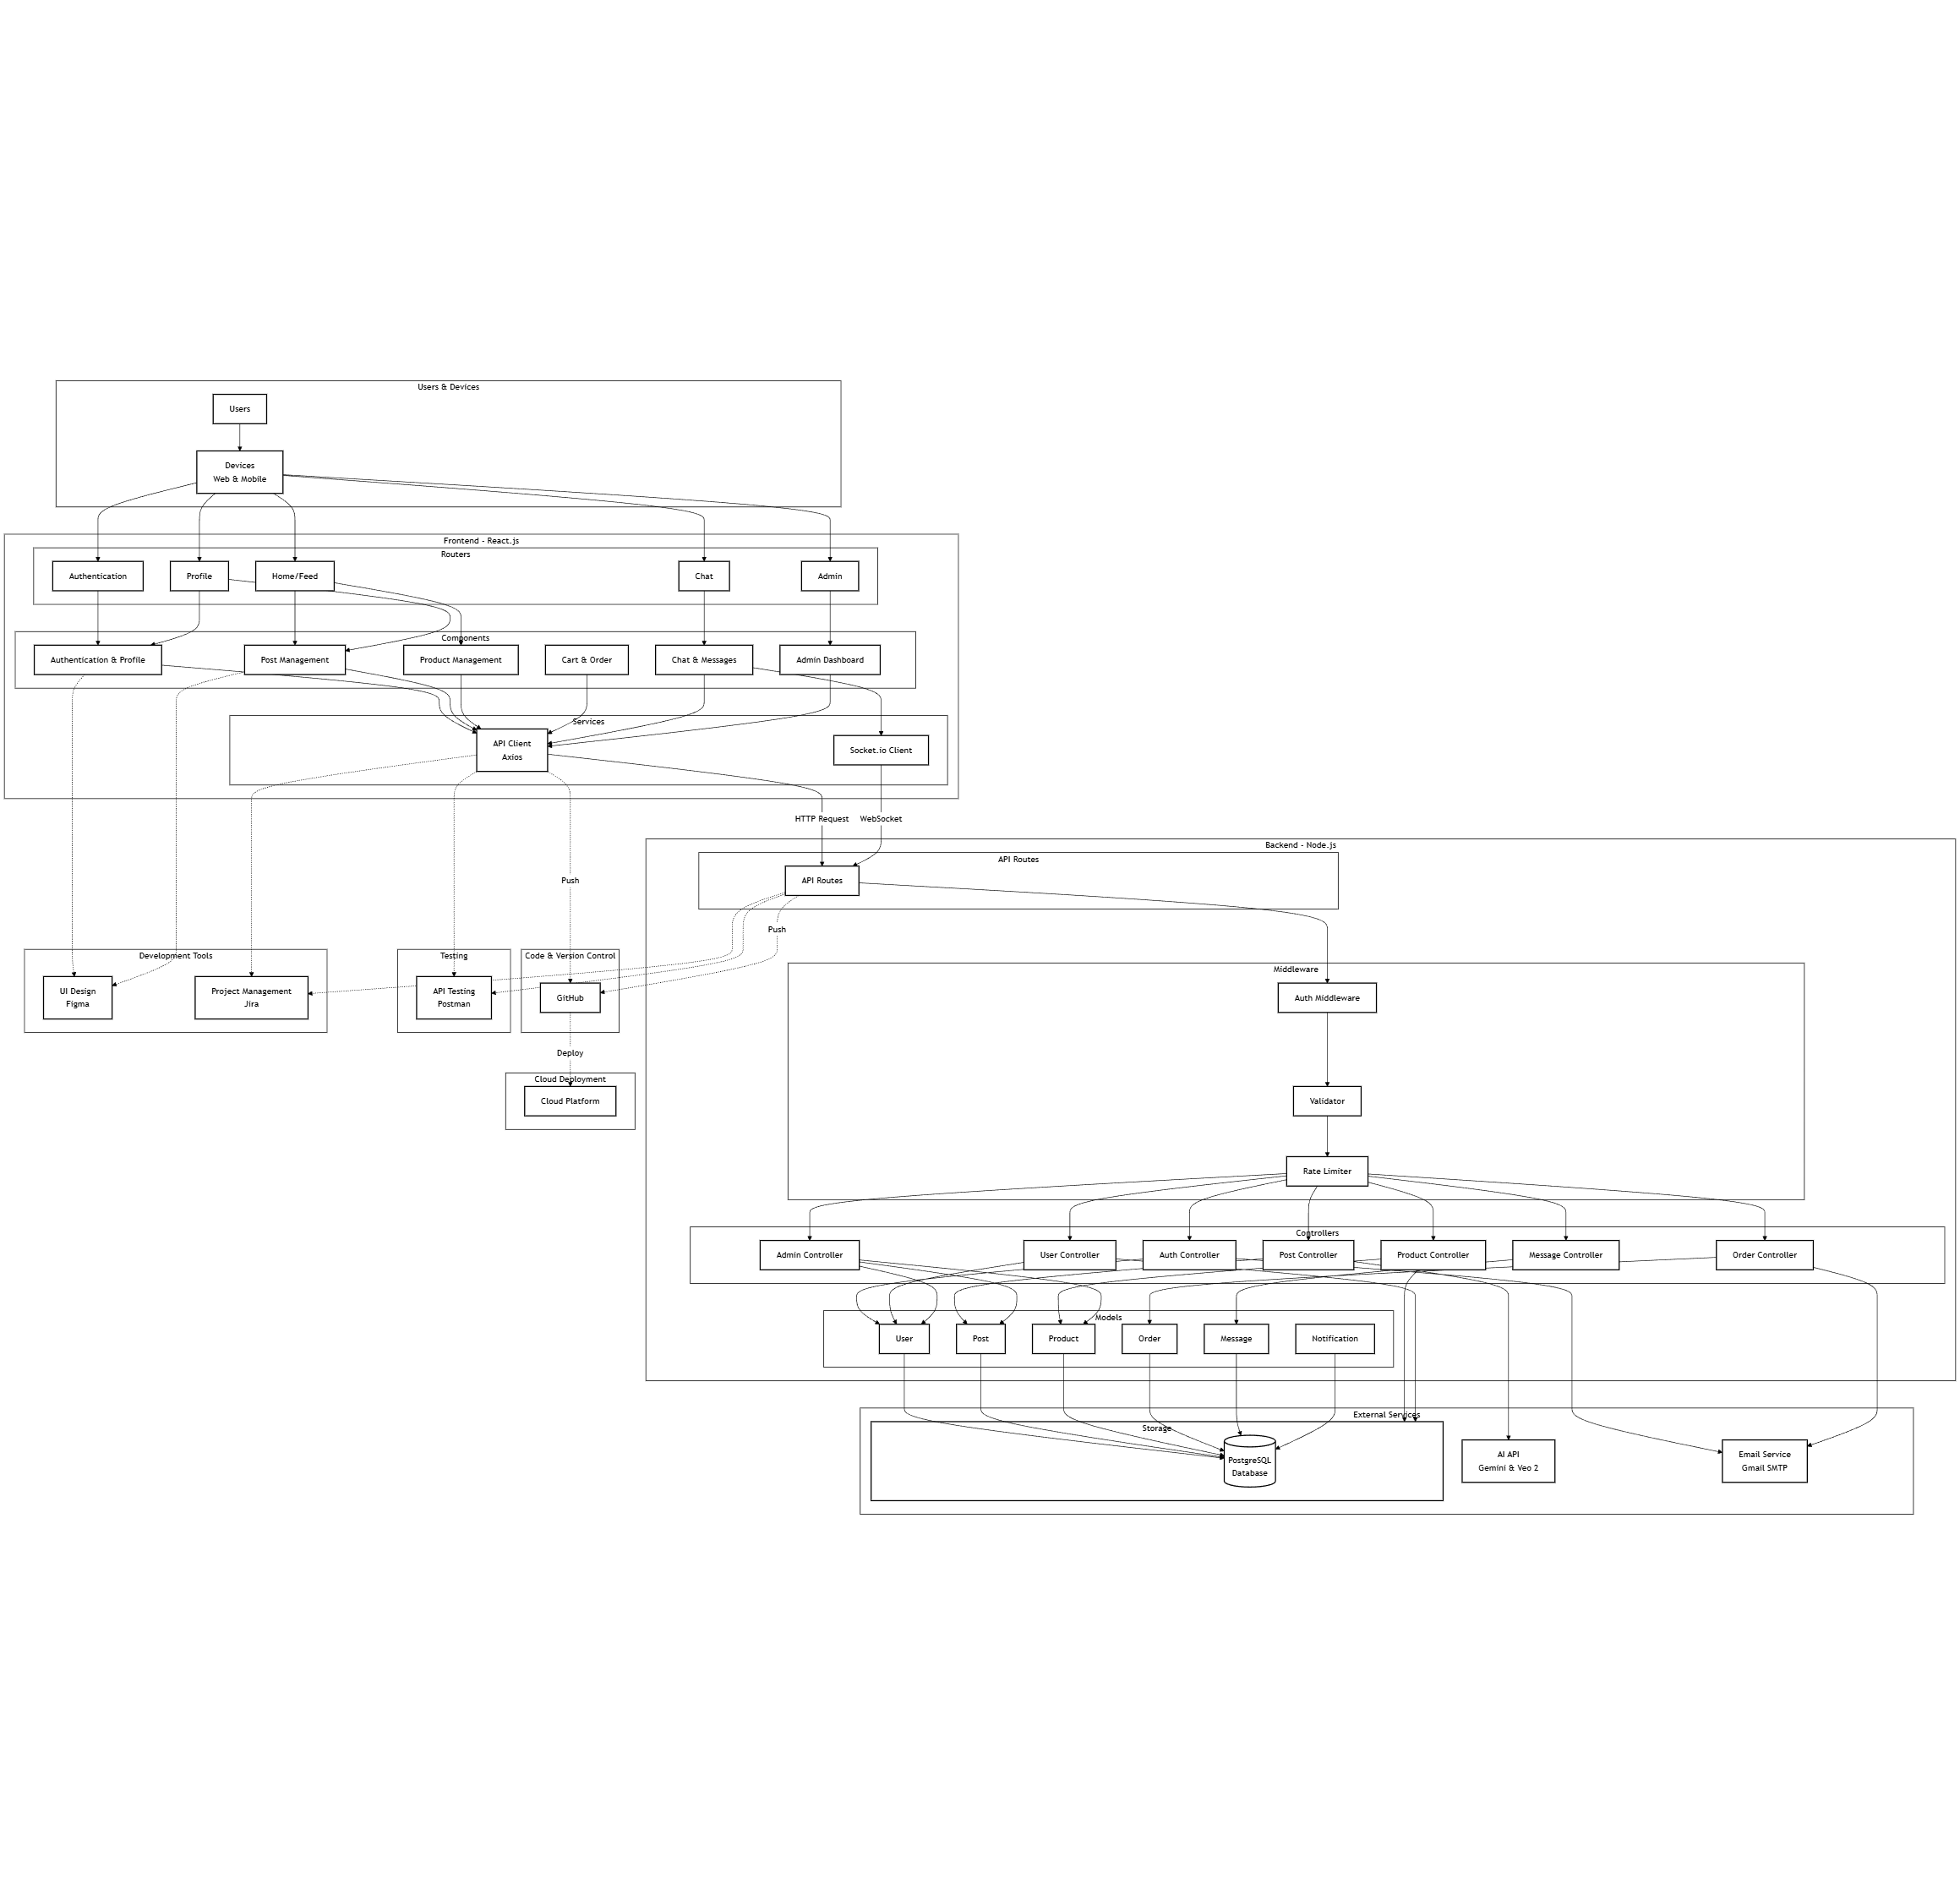
\includegraphics[width=1.0\textwidth]{Images/Architecture Diagram.png}
    \caption{Architecture Diagram for the system}
    \label{fig:architecture-diagram}
\end{figure}

\paragraph{Frontend Structure} Cấu trúc \textbf{Frontend} được tổ chức thành các thành phần chính:

\begin{itemize}
    \item \textbf{Routers}: Quản lý navigation giữa các trang
    \begin{itemize}
        \item \textbf{Authentication}: Trang xác thực người dùng
        \item \textbf{Home/Feed}: Trang chủ và bảng tin
        \item \textbf{Profile}: Trang hồ sơ người dùng
        \item \textbf{Chat}: Trang nhắn tin
        \item \textbf{Admin}: Trang quản trị
    \end{itemize}
    \item \textbf{Components}: Được tổ chức theo chức năng
    \begin{itemize}
        \item \textbf{Authentication \& Profile}: Xác thực và quản lý hồ sơ
        \item \textbf{Post Management}: Quản lý bài viết
        \item \textbf{Product Management}: Quản lý sản phẩm
        \item \textbf{Cart \& Order}: Giỏ hàng và đơn hàng
        \item \textbf{Chat \& Messages}: Tin nhắn và cuộc trò chuyện
        \item \textbf{Admin Dashboard}: Bảng điều khiển quản trị
    \end{itemize}
    \item \textbf{Services}: Kết nối với Backend
    \begin{itemize}
        \item \textbf{API Client (Axios)}: Thực hiện \textbf{HTTP request}
        \item \textbf{Socket.io Client}: Thiết lập kết nối \textbf{WebSocket} cho các tính năng \textbf{real-time}
    \end{itemize}
\end{itemize}

\paragraph{Backend Structure} \textbf{Backend} được xây dựng bằng \textbf{Node.js} với \textbf{Express.js framework}. Cấu trúc bao gồm:

\begin{itemize}
    \item \textbf{API Routes}: Đóng vai trò \textbf{entry point} nhận các request từ \textbf{Frontend}
    \item \textbf{Middleware}: Xử lý request qua chuỗi middleware
    \begin{itemize}
        \item \textbf{Auth Middleware}: Xác thực \textbf{JWT} và quản lý \textbf{session}
        \item \textbf{Validator}: Kiểm tra và validate dữ liệu đầu vào
        \item \textbf{Rate Limiter}: Giới hạn số lượng request để bảo vệ hệ thống
    \end{itemize}
    \item \textbf{Controllers}: Xử lý logic nghiệp vụ
    \begin{itemize}
        \item \textbf{Auth Controller}: Xử lý xác thực
        \item \textbf{User Controller}: Quản lý người dùng
        \item \textbf{Post Controller}: Quản lý bài viết
        \item \textbf{Product Controller}: Quản lý sản phẩm
        \item \textbf{Order Controller}: Quản lý đơn hàng
        \item \textbf{Message Controller}: Quản lý tin nhắn
        \item \textbf{Admin Controller}: Quản lý quản trị
    \end{itemize}
    \item \textbf{Models}: Đại diện cho các entity trong hệ thống
    \begin{itemize}
        \item \textbf{User}: Người dùng
        \item \textbf{Post}: Bài viết
        \item \textbf{Product}: Sản phẩm
        \item \textbf{Order}: Đơn hàng
        \item \textbf{Message}: Tin nhắn
        \item \textbf{Notification}: Thông báo
        \item Các Model hỗ trợ khác
    \end{itemize}
\end{itemize}

\paragraph{Database} Các \textbf{Model} này kết nối trực tiếp với database \textbf{PostgreSQL} thông qua \textbf{Sequelize ORM} để thực hiện các thao tác \textbf{CRUD} (Create, Read, Update, Delete).

\paragraph{Code \& Version Control} Để quản lý code và version, nhóm sử dụng \textbf{GitHub} và từ đó chúng tôi lên kế hoạch triển khai website thông qua \textbf{Cloud Platform} sử dụng các dịch vụ:

\begin{itemize}
    \item \textbf{Elastic Beanstalk}: Triển khai và quản lý ứng dụng
    \item \textbf{CodePipeline}: Tự động hóa quy trình CI/CD
    \item \textbf{Amazon RDS}: Quản lý database
\end{itemize}

Tất cả đều được cung cấp bởi các nhà cung cấp cloud.

\paragraph{Testing \& Development Tools} Hệ thống sử dụng các công cụ hỗ trợ:

\begin{itemize}
    \item \textbf{Testing}:
    \begin{itemize}
        \item \textbf{Postman}: Kiểm tra và đánh giá \textbf{API}
    \end{itemize}
    \item \textbf{Development Tools}:
    \begin{itemize}
        \item \textbf{Jira Software}: Bug tracking và project management
    \end{itemize}
\end{itemize}

\paragraph{External Services} Hệ thống tích hợp với các dịch vụ bên ngoài:

\begin{itemize}
    \item \textbf{AI API (Google Gemini \& Veo 2)}: Tạo nội dung đa phương thức (văn bản, hình ảnh, video ngắn)
    \item \textbf{File Storage (Cloudinary)}: Lưu trữ và quản lý hình ảnh
    \item \textbf{Email Service (Gmail SMTP)}: Gửi email xác thực và thông báo
\end{itemize}


\section{Thiết kế Pipeline AI Content Generation}
Phần này trình bày chi tiết thiết kế pipeline tạo nội dung AI cho hệ thống Social Commerce, bao gồm quy trình xây dựng prompt, tiêu chí đánh giá chất lượng kết quả, và chiến lược cải thiện khi kết quả chưa đạt yêu cầu.

\subsection{Tổng quan Pipeline}

Pipeline tạo nội dung AI được thiết kế theo mô hình \textbf{vòng lặp đánh giá -- cải thiện (Evaluate--Refine Loop)}, đảm bảo chất lượng đầu ra trước khi trả kết quả cho người dùng. Pipeline gồm 7 giai đoạn chính:

\begin{enumerate}
    \item \textbf{Thu nhận đầu vào (Input Collection)}: Thu thập mô tả, ý tưởng, hình ảnh tham khảo và ngữ cảnh từ người dùng.
    \item \textbf{Phân tích đầu vào (Input Analysis)}: Trích xuất thực thể, xác định giọng điệu, phân loại nội dung.
    \item \textbf{Xây dựng Prompt (Prompt Construction)}: Tổng hợp tất cả thông tin thành prompt có cấu trúc gửi đến API.
    \item \textbf{Gọi API (API Invocation)}: Gửi prompt đến Google Gemini API (văn bản, hình ảnh) hoặc Google Veo 2 (video).
    \item \textbf{Đánh giá chất lượng (Quality Evaluation)}: Chấm điểm kết quả theo các tiêu chí đã định nghĩa.
    \item \textbf{Quyết định và Cải thiện (Decision \& Refinement)}: Nếu đạt ngưỡng thì trả kết quả; nếu chưa đạt thì sửa prompt và thử lại (tối đa 3 lần).
    \item \textbf{Trả kết quả và Hỗ trợ chỉnh sửa (Result Delivery \& Editing Support)}: Hiển thị kết quả kèm điểm đánh giá và gợi ý chỉnh sửa cho người dùng.
\end{enumerate}

% TODO: Thêm hình minh họa pipeline tổng quan
% \begin{figure}[H]
%   \centering
%   \includegraphics[width=\textwidth]{Images/AI-Pipeline-Overview.png}
%   \caption{Tổng quan Pipeline tạo nội dung AI}
%   \label{fig:ai-pipeline-overview}
% \end{figure}

Luồng xử lý tổng quát như sau: Khi người dùng gửi yêu cầu tạo nội dung, hệ thống phân tích đầu vào để hiểu ngữ cảnh và ý định, sau đó xây dựng prompt tối ưu cho từng loại nội dung (văn bản, hình ảnh, video). Kết quả từ API được đánh giá tự động bằng kết hợp \textbf{kiểm tra quy tắc (rule-based checks)} và \textbf{đánh giá bằng AI (AI-based evaluation)}. Nếu điểm đánh giá dưới ngưỡng chấp nhận, hệ thống tự động phân tích điểm yếu, bổ sung ràng buộc vào prompt và gọi lại API. Quy trình lặp tối đa 3 lần trước khi trả về kết quả tốt nhất kèm gợi ý chỉnh sửa.

\subsection{Phân tích đầu vào (Input Analysis)}

Trước khi xây dựng prompt, hệ thống thực hiện phân tích đầu vào để trích xuất thông tin có cấu trúc:

\begin{table}[H]
\centering
\renewcommand{\arraystretch}{1.3}
\begin{tabularx}{\textwidth}{|l|X|}
\hline
\textbf{Thông tin} & \textbf{Mô tả} \\ \hline
Thực thể chính & Tên sản phẩm, đặc điểm nổi bật, lợi ích, giá cả (nếu có) được trích xuất từ mô tả của người dùng. \\ \hline
Loại nội dung & Phân loại mục đích: quảng cáo sản phẩm, chia sẻ trải nghiệm, thông tin giáo dục, giải trí, hoặc kết hợp. \\ \hline
Đối tượng mục tiêu & Xác định từ ngữ cảnh: thông tin hồ sơ người bán, danh mục sản phẩm, lịch sử bài đăng. \\ \hline
Giọng điệu & Xác định từ từ khóa trong mô tả: chuyên nghiệp, thân thiện, hài hước, sang trọng, trẻ trung. \\ \hline
Thông tin hình ảnh & Nếu có hình ảnh đầu vào: sử dụng Gemini Vision phân tích nội dung hình ảnh, màu sắc chủ đạo, đối tượng trong ảnh. \\ \hline
Ngữ cảnh thương hiệu & Lấy từ hồ sơ shop của Seller: tên shop, phong cách, danh mục sản phẩm chính, tone \& voice. \\ \hline
\end{tabularx}
\caption{Các thông tin được trích xuất trong giai đoạn Phân tích đầu vào}
\label{tab:input-analysis}
\end{table}

\subsection{Xây dựng Prompt (Prompt Engineering)}

\subsubsection{Cấu trúc Prompt tổng quát}

Mỗi prompt gửi đến Google Gemini API được xây dựng theo cấu trúc 5 phần:

\begin{enumerate}
    \item \textbf{System Instruction}: Định nghĩa vai trò và hành vi của AI (không thay đổi giữa các lần gọi).
    \item \textbf{Context Block}: Ngữ cảnh nền tảng (Social Commerce), thông tin thương hiệu, đối tượng mục tiêu.
    \item \textbf{User Input Block}: Mô tả, ý tưởng và hình ảnh tham khảo từ người dùng.
    \item \textbf{Constraint Block}: Các ràng buộc về độ dài, giọng điệu, định dạng đầu ra, nội dung cần tránh.
    \item \textbf{Output Format Specification}: Định dạng JSON cụ thể cho đầu ra để dễ parse và đánh giá.
\end{enumerate}

\subsubsection{Prompt cho nội dung văn bản (Text Generation)}

Prompt tạo văn bản được thiết kế để sinh ra bài viết hoàn chỉnh cho nền tảng Social Commerce:

\begin{table}[H]
\centering
\renewcommand{\arraystretch}{1.3}
\begin{tabularx}{\textwidth}{|l|X|}
\hline
\textbf{Thành phần} & \textbf{Nội dung} \\ \hline
System Instruction & ``Bạn là chuyên gia sáng tạo nội dung cho nền tảng Social Commerce. Nhiệm vụ: tạo bài viết hấp dẫn, thúc đẩy tương tác và chuyển đổi mua hàng.'' \\ \hline
Context & Tên shop, danh mục sản phẩm, phong cách thương hiệu, nền tảng (Social Commerce với tính năng mua sắm trực tiếp). \\ \hline
User Input & Mô tả/ý tưởng người dùng + kết quả phân tích hình ảnh (nếu có). \\ \hline
Constraints & Độ dài: 100--300 từ; Hashtag: 5--10 cái liên quan; Phải có Call-to-Action; Ngôn ngữ: tiếng Việt; Không sử dụng nội dung nhạy cảm. \\ \hline
Output Format & JSON: \texttt{\{title, body, hashtags[], callToAction, tone\}}. \\ \hline
\end{tabularx}
\caption{Cấu trúc Prompt cho Text Generation}
\label{tab:prompt-text}
\end{table}

\subsubsection{Prompt cho hình ảnh (Image Generation)}

Prompt tạo hình ảnh được xây dựng dựa trên nội dung văn bản đã tạo và ngữ cảnh sản phẩm:

\begin{table}[H]
\centering
\renewcommand{\arraystretch}{1.3}
\begin{tabularx}{\textwidth}{|l|X|}
\hline
\textbf{Thành phần} & \textbf{Nội dung} \\ \hline
System Instruction & ``Tạo hình ảnh quảng cáo chất lượng cao cho nền tảng Social Commerce. Hình ảnh phải bắt mắt, phù hợp với nội dung bài viết và phong cách thương hiệu.'' \\ \hline
Context & Nội dung bài viết đã tạo (hoặc đang tạo song song), thông tin sản phẩm, phong cách thương hiệu. \\ \hline
Visual Spec & Phong cách hình ảnh (photorealistic, illustration, minimalist, etc.), bảng màu chủ đạo, bố cục mong muốn. \\ \hline
Constraints & Tỷ lệ: 1:1 hoặc 4:5 (phù hợp social media); Không chứa text/watermark không mong muốn; Phù hợp với nội dung đã tạo. \\ \hline
Negative Prompt & Nội dung cần tránh: hình ảnh mờ, biến dạng, không phù hợp, vi phạm bản quyền. \\ \hline
\end{tabularx}
\caption{Cấu trúc Prompt cho Image Generation}
\label{tab:prompt-image}
\end{table}

\subsubsection{Prompt cho video (Video Generation)}

Prompt tạo video sử dụng Google Veo 2 được thiết kế dựa trên storyboard tự động:

\begin{table}[H]
\centering
\renewcommand{\arraystretch}{1.3}
\begin{tabularx}{\textwidth}{|l|X|}
\hline
\textbf{Thành phần} & \textbf{Nội dung} \\ \hline
System Instruction & ``Tạo video ngắn quảng cáo hấp dẫn cho nền tảng Social Commerce. Video phải thu hút sự chú ý trong 3 giây đầu tiên.'' \\ \hline
Context & Nội dung bài viết, hình ảnh đã tạo (làm keyframe tham chiếu), thông tin sản phẩm. \\ \hline
Storyboard & Mô tả các cảnh chính: cảnh mở đầu (hook), cảnh giới thiệu sản phẩm, cảnh highlight đặc điểm, cảnh Call-to-Action. \\ \hline
Constraints & Độ dài: 15--30 giây; Chuyển cảnh mượt; Phong cách nhất quán với hình ảnh đã tạo; Phù hợp cho xem trên thiết bị di động. \\ \hline
Technical Spec & Tỷ lệ: 9:16 (vertical) hoặc 1:1 (square); Tốc độ: phù hợp với nội dung; Không cần audio (sẽ thêm sau). \\ \hline
\end{tabularx}
\caption{Cấu trúc Prompt cho Video Generation}
\label{tab:prompt-video}
\end{table}

\subsection{Tiêu chí đánh giá chất lượng kết quả}

Sau khi nhận kết quả từ API, hệ thống thực hiện đánh giá chất lượng bằng phương pháp \textbf{kết hợp (hybrid)}: kiểm tra quy tắc tự động (rule-based) cho các tiêu chí có thể đo lường được, và sử dụng chính Gemini API để đánh giá các tiêu chí mang tính chủ quan (AI-based evaluation). Mỗi tiêu chí được chấm trên thang điểm \textbf{1--10}. Điểm tổng hợp là \textbf{trung bình có trọng số (weighted average)} và ngưỡng chấp nhận là \textbf{$\geq$ 7.0/10}.

\subsubsection{Tiêu chí đánh giá nội dung văn bản}

\begin{longtable}{|p{2.8cm}|p{5cm}|p{1.2cm}|p{4.5cm}|}
\caption{Tiêu chí đánh giá chất lượng nội dung văn bản} \label{tab:eval-text} \\
\hline
\textbf{Tiêu chí} & \textbf{Mô tả} & \textbf{Trọng số} & \textbf{Phương pháp đánh giá} \\ \hline
\endfirsthead

\multicolumn{4}{c}%
{{\bfseries \tablename\ \thetable{} -- tiếp tục từ trang trước}} \\
\hline
\textbf{Tiêu chí} & \textbf{Mô tả} & \textbf{Trọng số} & \textbf{Phương pháp đánh giá} \\ \hline
\endhead

\hline \multicolumn{4}{|r|}{{Tiếp tục ở trang sau}} \\ \hline
\endfoot

\hline
\endlastfoot

Tính liên quan (Relevance) & Nội dung phù hợp với mô tả, ý tưởng và hình ảnh đầu vào của người dùng. & 0.25 & AI-based: Gemini so sánh ngữ nghĩa giữa đầu vào và đầu ra. \\ \hline
Tính hấp dẫn (Engagement) & Nội dung có sức hút, có hook cảm xúc, câu hỏi gợi mở, hoặc Call-to-Action rõ ràng. & 0.20 & AI-based: Gemini đánh giá engagement potential. \\ \hline
Cấu trúc hoàn chỉnh (Structure) & Có đầy đủ tiêu đề, nội dung chính, hashtags theo đúng format yêu cầu. & 0.15 & Rule-based: Kiểm tra sự hiện diện của từng trường trong JSON output. \\ \hline
Độ dài phù hợp (Length) & Nội dung nằm trong khoảng 100--300 từ, phù hợp nền tảng social media. & 0.10 & Rule-based: Đếm số từ, so sánh với khoảng cho phép. \\ \hline
Chất lượng ngôn ngữ (Language) & Ngữ pháp chính xác, văn phong tự nhiên, giọng điệu phù hợp với yêu cầu. & 0.15 & AI-based: Gemini đánh giá grammar và naturalness. \\ \hline
Giá trị thương mại (Commercial Value) & Nếu là bài bán hàng: phải highlight lợi ích sản phẩm, tạo nhu cầu mua, có CTA mua hàng. & 0.15 & AI-based: Gemini đánh giá persuasion và commercial intent. \\ \hline
\end{longtable}

\subsubsection{Tiêu chí đánh giá hình ảnh}

\begin{longtable}{|p{2.8cm}|p{5cm}|p{1.2cm}|p{4.5cm}|}
\caption{Tiêu chí đánh giá chất lượng hình ảnh} \label{tab:eval-image} \\
\hline
\textbf{Tiêu chí} & \textbf{Mô tả} & \textbf{Trọng số} & \textbf{Phương pháp đánh giá} \\ \hline
\endfirsthead

\multicolumn{4}{c}%
{{\bfseries \tablename\ \thetable{} -- tiếp tục từ trang trước}} \\
\hline
\textbf{Tiêu chí} & \textbf{Mô tả} & \textbf{Trọng số} & \textbf{Phương pháp đánh giá} \\ \hline
\endhead

\hline \multicolumn{4}{|r|}{{Tiếp tục ở trang sau}} \\ \hline
\endfoot

\hline
\endlastfoot

Tính liên quan (Relevance) & Hình ảnh phù hợp với nội dung bài viết và sản phẩm được mô tả. & 0.30 & AI-based: Gemini Vision phân tích hình ảnh và so sánh với context. \\ \hline
Chất lượng kỹ thuật (Technical Quality) & Độ phân giải đủ cao, không bị mờ, méo, artifact; tỷ lệ khung hình phù hợp. & 0.25 & Rule-based: Kiểm tra resolution, aspect ratio. AI-based: Kiểm tra artifact. \\ \hline
Tính thẩm mỹ (Aesthetic) & Bố cục cân đối, màu sắc hài hòa, ánh sáng tự nhiên, tổng thể bắt mắt. & 0.25 & AI-based: Gemini Vision đánh giá aesthetic quality. \\ \hline
Nhất quán thương hiệu (Brand Consistency) & Phong cách hình ảnh phù hợp với tone của thương hiệu và các hình ảnh khác trong bài. & 0.20 & AI-based: Gemini so sánh style với brand profile. \\ \hline
\end{longtable}

\subsubsection{Tiêu chí đánh giá video}

\begin{longtable}{|p{2.8cm}|p{5cm}|p{1.2cm}|p{4.5cm}|}
\caption{Tiêu chí đánh giá chất lượng video} \label{tab:eval-video} \\
\hline
\textbf{Tiêu chí} & \textbf{Mô tả} & \textbf{Trọng số} & \textbf{Phương pháp đánh giá} \\ \hline
\endfirsthead

\multicolumn{4}{c}%
{{\bfseries \tablename\ \thetable{} -- tiếp tục từ trang trước}} \\
\hline
\textbf{Tiêu chí} & \textbf{Mô tả} & \textbf{Trọng số} & \textbf{Phương pháp đánh giá} \\ \hline
\endhead

\hline \multicolumn{4}{|r|}{{Tiếp tục ở trang sau}} \\ \hline
\endfoot

\hline
\endlastfoot

Tính mạch lạc (Coherence) & Nội dung video logic, mạch lạc, có cấu trúc mở đầu -- thân -- kết. & 0.25 & AI-based: Gemini phân tích các frame chính và đánh giá narrative flow. \\ \hline
Chất lượng hình ảnh (Visual Quality) & Chuyển cảnh mượt mà, hình ảnh sắc nét, không bị giật hoặc biến dạng. & 0.25 & AI-based: Gemini đánh giá visual quality trên các frame trích xuất. \\ \hline
Độ dài phù hợp (Duration) & Video nằm trong khoảng 15--30 giây, phù hợp cho social media. & 0.15 & Rule-based: Kiểm tra duration metadata. \\ \hline
Tính hấp dẫn (Engagement) & Thu hút sự chú ý ngay từ đầu (3 giây đầu), nội dung compelling, kết thúc ấn tượng. & 0.20 & AI-based: Gemini đánh giá hook strength và overall engagement. \\ \hline
Nhất quán nội dung (Content Consistency) & Phong cách video nhất quán với hình ảnh và bài viết đã tạo trong cùng bài đăng. & 0.15 & AI-based: Gemini so sánh style giữa video, hình ảnh và text. \\ \hline
\end{longtable}

\subsubsection{Quy trình đánh giá tự động}

Quy trình đánh giá được thực hiện theo hai bước:

\textbf{Bước 1 -- Kiểm tra quy tắc (Rule-based Checks):} Hệ thống thực hiện các kiểm tra tự động có thể lập trình được:
\begin{itemize}
    \item Kiểm tra định dạng JSON output có đúng schema yêu cầu.
    \item Kiểm tra độ dài nội dung văn bản (100--300 từ).
    \item Kiểm tra số lượng hashtag (5--10).
    \item Kiểm tra sự hiện diện của Call-to-Action.
    \item Kiểm tra tỷ lệ khung hình và độ phân giải hình ảnh.
    \item Kiểm tra độ dài video (15--30 giây).
\end{itemize}

Nếu bất kỳ kiểm tra rule-based nào thất bại, tiêu chí tương ứng tự động nhận điểm thấp (1--3) mà không cần gọi AI đánh giá, giúp tiết kiệm chi phí API.

\textbf{Bước 2 -- Đánh giá bằng AI (AI-based Evaluation):} Đối với các tiêu chí mang tính chủ quan, hệ thống gửi một prompt đánh giá đến Gemini API với cấu trúc:

\begin{itemize}
    \item \textbf{Input}: Đầu vào gốc của người dùng + kết quả vừa tạo.
    \item \textbf{Rubric}: Bảng tiêu chí đánh giá với mô tả chi tiết cho từng mức điểm.
    \item \textbf{Output}: JSON chứa điểm số (1--10) và lý do ngắn gọn cho từng tiêu chí.
\end{itemize}

Điểm tổng hợp được tính theo công thức:

\[
\text{Score}_{total} = \sum_{i=1}^{n} w_i \times s_i
\]

trong đó $w_i$ là trọng số và $s_i$ là điểm của tiêu chí thứ $i$. Nếu $\text{Score}_{total} \geq 7.0$, kết quả được coi là đạt yêu cầu.

\subsection{Chiến lược cải thiện kết quả}

Khi điểm đánh giá tổng hợp $< 7.0/10$, hệ thống thực hiện cải thiện tự động theo chiến lược phân tầng:

\subsubsection{Tự động sửa Prompt (Automatic Prompt Refinement)}

Quy trình sửa prompt tự động gồm 3 bước:

\textbf{Bước 1 -- Xác định điểm yếu:} Hệ thống phân tích kết quả đánh giá, xác định tiêu chí nào có điểm thấp nhất (dưới 6/10). Ví dụ: nếu tiêu chí ``Tính hấp dẫn'' chỉ đạt 4/10, đây là tiêu chí cần cải thiện ưu tiên.

\textbf{Bước 2 -- Sinh ràng buộc bổ sung:} Dựa trên tiêu chí yếu, hệ thống áp dụng bảng ánh xạ sau để bổ sung ràng buộc vào prompt:

\begin{longtable}{|p{3cm}|p{5.5cm}|p{5cm}|}
\caption{Ánh xạ tiêu chí yếu $\rightarrow$ Ràng buộc bổ sung cho Prompt} \label{tab:refinement-map} \\
\hline
\textbf{Tiêu chí yếu} & \textbf{Ràng buộc bổ sung vào Prompt} & \textbf{Ví dụ} \\ \hline
\endfirsthead

\multicolumn{3}{c}%
{{\bfseries \tablename\ \thetable{} -- tiếp tục từ trang trước}} \\
\hline
\textbf{Tiêu chí yếu} & \textbf{Ràng buộc bổ sung vào Prompt} & \textbf{Ví dụ} \\ \hline
\endhead

\hline \multicolumn{3}{|r|}{{Tiếp tục ở trang sau}} \\ \hline
\endfoot

\hline
\endlastfoot

Tính liên quan thấp & Thêm câu: ``Bài viết PHẢI đề cập trực tiếp đến: [danh sách thực thể chính].'' Kèm theo kết quả trước đó và lý do không liên quan. & ``Bài viết PHẢI đề cập trực tiếp đến: kem chống nắng, SPF 50+, bảo vệ da.'' \\ \hline
Tính hấp dẫn thấp & Thêm: ``Bắt đầu bằng câu hỏi gợi mở hoặc số liệu ấn tượng. Thêm ít nhất 2 emoji liên quan. Kết thúc bằng CTA mạnh mẽ.'' & ``Bạn có biết 80\% người dùng...?'' \\ \hline
Cấu trúc chưa đạt & Thêm: ``Output PHẢI tuân thủ chính xác JSON schema sau: [schema]. Mỗi trường là BẮT BUỘC.'' & Nhấn mạnh format và ví dụ output mong muốn. \\ \hline
Ngôn ngữ chưa tốt & Thêm: ``Viết bằng tiếng Việt tự nhiên, tránh dịch máy. Giọng điệu [tone cụ thể]. Không sử dụng thuật ngữ quá chuyên môn.'' & ``Giọng điệu thân thiện, gần gũi như đang tư vấn cho bạn bè.'' \\ \hline
Giá trị thương mại thấp & Thêm: ``Highlight rõ ràng 3 lợi ích chính của sản phẩm. Tạo cảm giác khan hiếm hoặc ưu đãi. Đưa ra lý do nên mua ngay.'' & ``Ưu đãi chỉ còn 2 ngày! Mua ngay để nhận...'' \\ \hline
Hình ảnh không liên quan & Bổ sung mô tả chi tiết hơn về đối tượng chính cần xuất hiện trong ảnh, kèm negative prompt mạnh hơn. & ``Hình ảnh PHẢI chứa lọ kem chống nắng ở vị trí trung tâm, nền biển hoặc ngoài trời.'' \\ \hline
Video thiếu mạch lạc & Bổ sung storyboard chi tiết hơn với mô tả từng cảnh cụ thể, thời lượng từng cảnh, và chuyển cảnh. & ``Cảnh 1 (0--5s): Cận ảnh sản phẩm. Cảnh 2 (5--15s): Demo sử dụng...'' \\ \hline
\end{longtable}

\textbf{Bước 3 -- Gọi lại API:} Hệ thống gửi prompt đã cải thiện đến API. Kết quả mới được đánh giá lại. Quá trình lặp tối đa \textbf{3 lần (max\_retries = 3)}. Sau mỗi lần lặp, hệ thống theo dõi xem điểm có cải thiện hay không. Nếu điểm không cải thiện sau 2 lần liên tiếp, hệ thống dừng lặp sớm để tránh lãng phí tài nguyên.

\subsubsection{Hỗ trợ chỉnh sửa trực tiếp bởi người dùng}

Sau khi pipeline tự động hoàn tất (dù đạt hay chưa đạt ngưỡng), kết quả được trả về cho người dùng kèm theo:

\begin{itemize}
    \item \textbf{Điểm đánh giá chi tiết}: Hiển thị điểm từng tiêu chí và điểm tổng hợp dưới dạng trực quan (thanh tiến trình hoặc biểu đồ radar).
    \item \textbf{Gợi ý cải thiện}: Dựa trên tiêu chí có điểm thấp, hệ thống gợi ý cụ thể cho người dùng.
    \item \textbf{Công cụ chỉnh sửa}: Tùy theo loại nội dung.
\end{itemize}

\textbf{Chỉnh sửa nội dung văn bản:}
\begin{itemize}
    \item Rich text editor cho phép chỉnh sửa trực tiếp tiêu đề, nội dung, hashtags.
    \item Nút ``Viết lại đoạn này'' cho phép chọn một phần nội dung và yêu cầu AI viết lại riêng đoạn đó với hướng dẫn cụ thể (ngắn hơn, hấp dẫn hơn, chuyên nghiệp hơn).
    \item Điều chỉnh giọng điệu: dropdown chọn tone (chuyên nghiệp, thân thiện, hài hước, sang trọng) để AI viết lại toàn bộ theo giọng điệu mới.
    \item Thêm/bớt hashtags thủ công hoặc yêu cầu AI gợi ý thêm.
\end{itemize}

\textbf{Chỉnh sửa hình ảnh:}
\begin{itemize}
    \item Tạo lại hình ảnh với mô tả cụ thể hơn (người dùng bổ sung yêu cầu).
    \item Chọn phong cách hình ảnh khác (photorealistic, illustration, flat design, etc.) và tạo lại.
    \item Giữ hình ảnh hiện tại nhưng yêu cầu AI chỉnh sửa cụ thể (thay đổi màu nền, thêm/bớt đối tượng).
    \item Tải lên hình ảnh thay thế từ thiết bị.
\end{itemize}

\textbf{Chỉnh sửa video:}
\begin{itemize}
    \item Tạo lại video với mô tả storyboard chi tiết hơn từ người dùng.
    \item Yêu cầu thay đổi tốc độ, phong cách, hoặc bố cục cảnh.
    \item Tạo lại chỉ một phần video (ví dụ: chỉ cảnh mở đầu).
    \item Tải lên video thay thế từ thiết bị.
\end{itemize}

\subsubsection{Tổng hợp luồng quyết định}

Toàn bộ luồng quyết định của pipeline được tóm tắt như sau:

\begin{enumerate}
    \item Nhận kết quả từ API $\rightarrow$ Đánh giá chất lượng.
    \item Nếu \textbf{Score $\geq$ 7.0}: Trả kết quả cho người dùng (trạng thái: \textit{Đạt yêu cầu}).
    \item Nếu \textbf{Score $<$ 7.0} và \textbf{retry $<$ max\_retries}:
    \begin{itemize}
        \item Xác định tiêu chí yếu nhất.
        \item Bổ sung ràng buộc tương ứng vào prompt.
        \item Gọi lại API $\rightarrow$ Quay lại bước 1.
    \end{itemize}
    \item Nếu \textbf{Score $<$ 7.0} và \textbf{retry $\geq$ max\_retries}:
    \begin{itemize}
        \item Chọn kết quả có điểm cao nhất trong tất cả các lần thử.
        \item Trả kết quả kèm gợi ý chỉnh sửa cụ thể (trạng thái: \textit{Cần chỉnh sửa}).
        \item Người dùng chỉnh sửa trực tiếp hoặc nhập thêm yêu cầu và tạo lại.
    \end{itemize}
\end{enumerate}

% TODO: Thêm hình minh họa luồng quyết định (flowchart)
% \begin{figure}[H]
%   \centering
%   \includegraphics[width=\textwidth]{Images/AI-Pipeline-Decision-Flow.png}
%   \caption{Luồng quyết định trong Pipeline AI Content Generation}
%   \label{fig:ai-pipeline-decision}
% \end{figure}


\section{Component diagram}
Component diagram mô tả cấu trúc và mối quan hệ giữa các thành phần trong hệ thống theo mô hình \textbf{MVCS}. Để dễ hiểu và quản lý, chúng tôi chia component diagram thành hai loại: \textbf{tổng quan} và \textbf{theo từng vai trò người dùng}.

\subsubsection{Component diagram tổng quan}

\ref{fig:component-overview} minh họa kiến trúc tổng quan của hệ thống, bao gồm frontend người dùng, core backend API, frontend admin, admin backend API, PostgreSQL, Redis cache và các dịch vụ ngoài.

\begin{figure}[htbp]
    \centering
    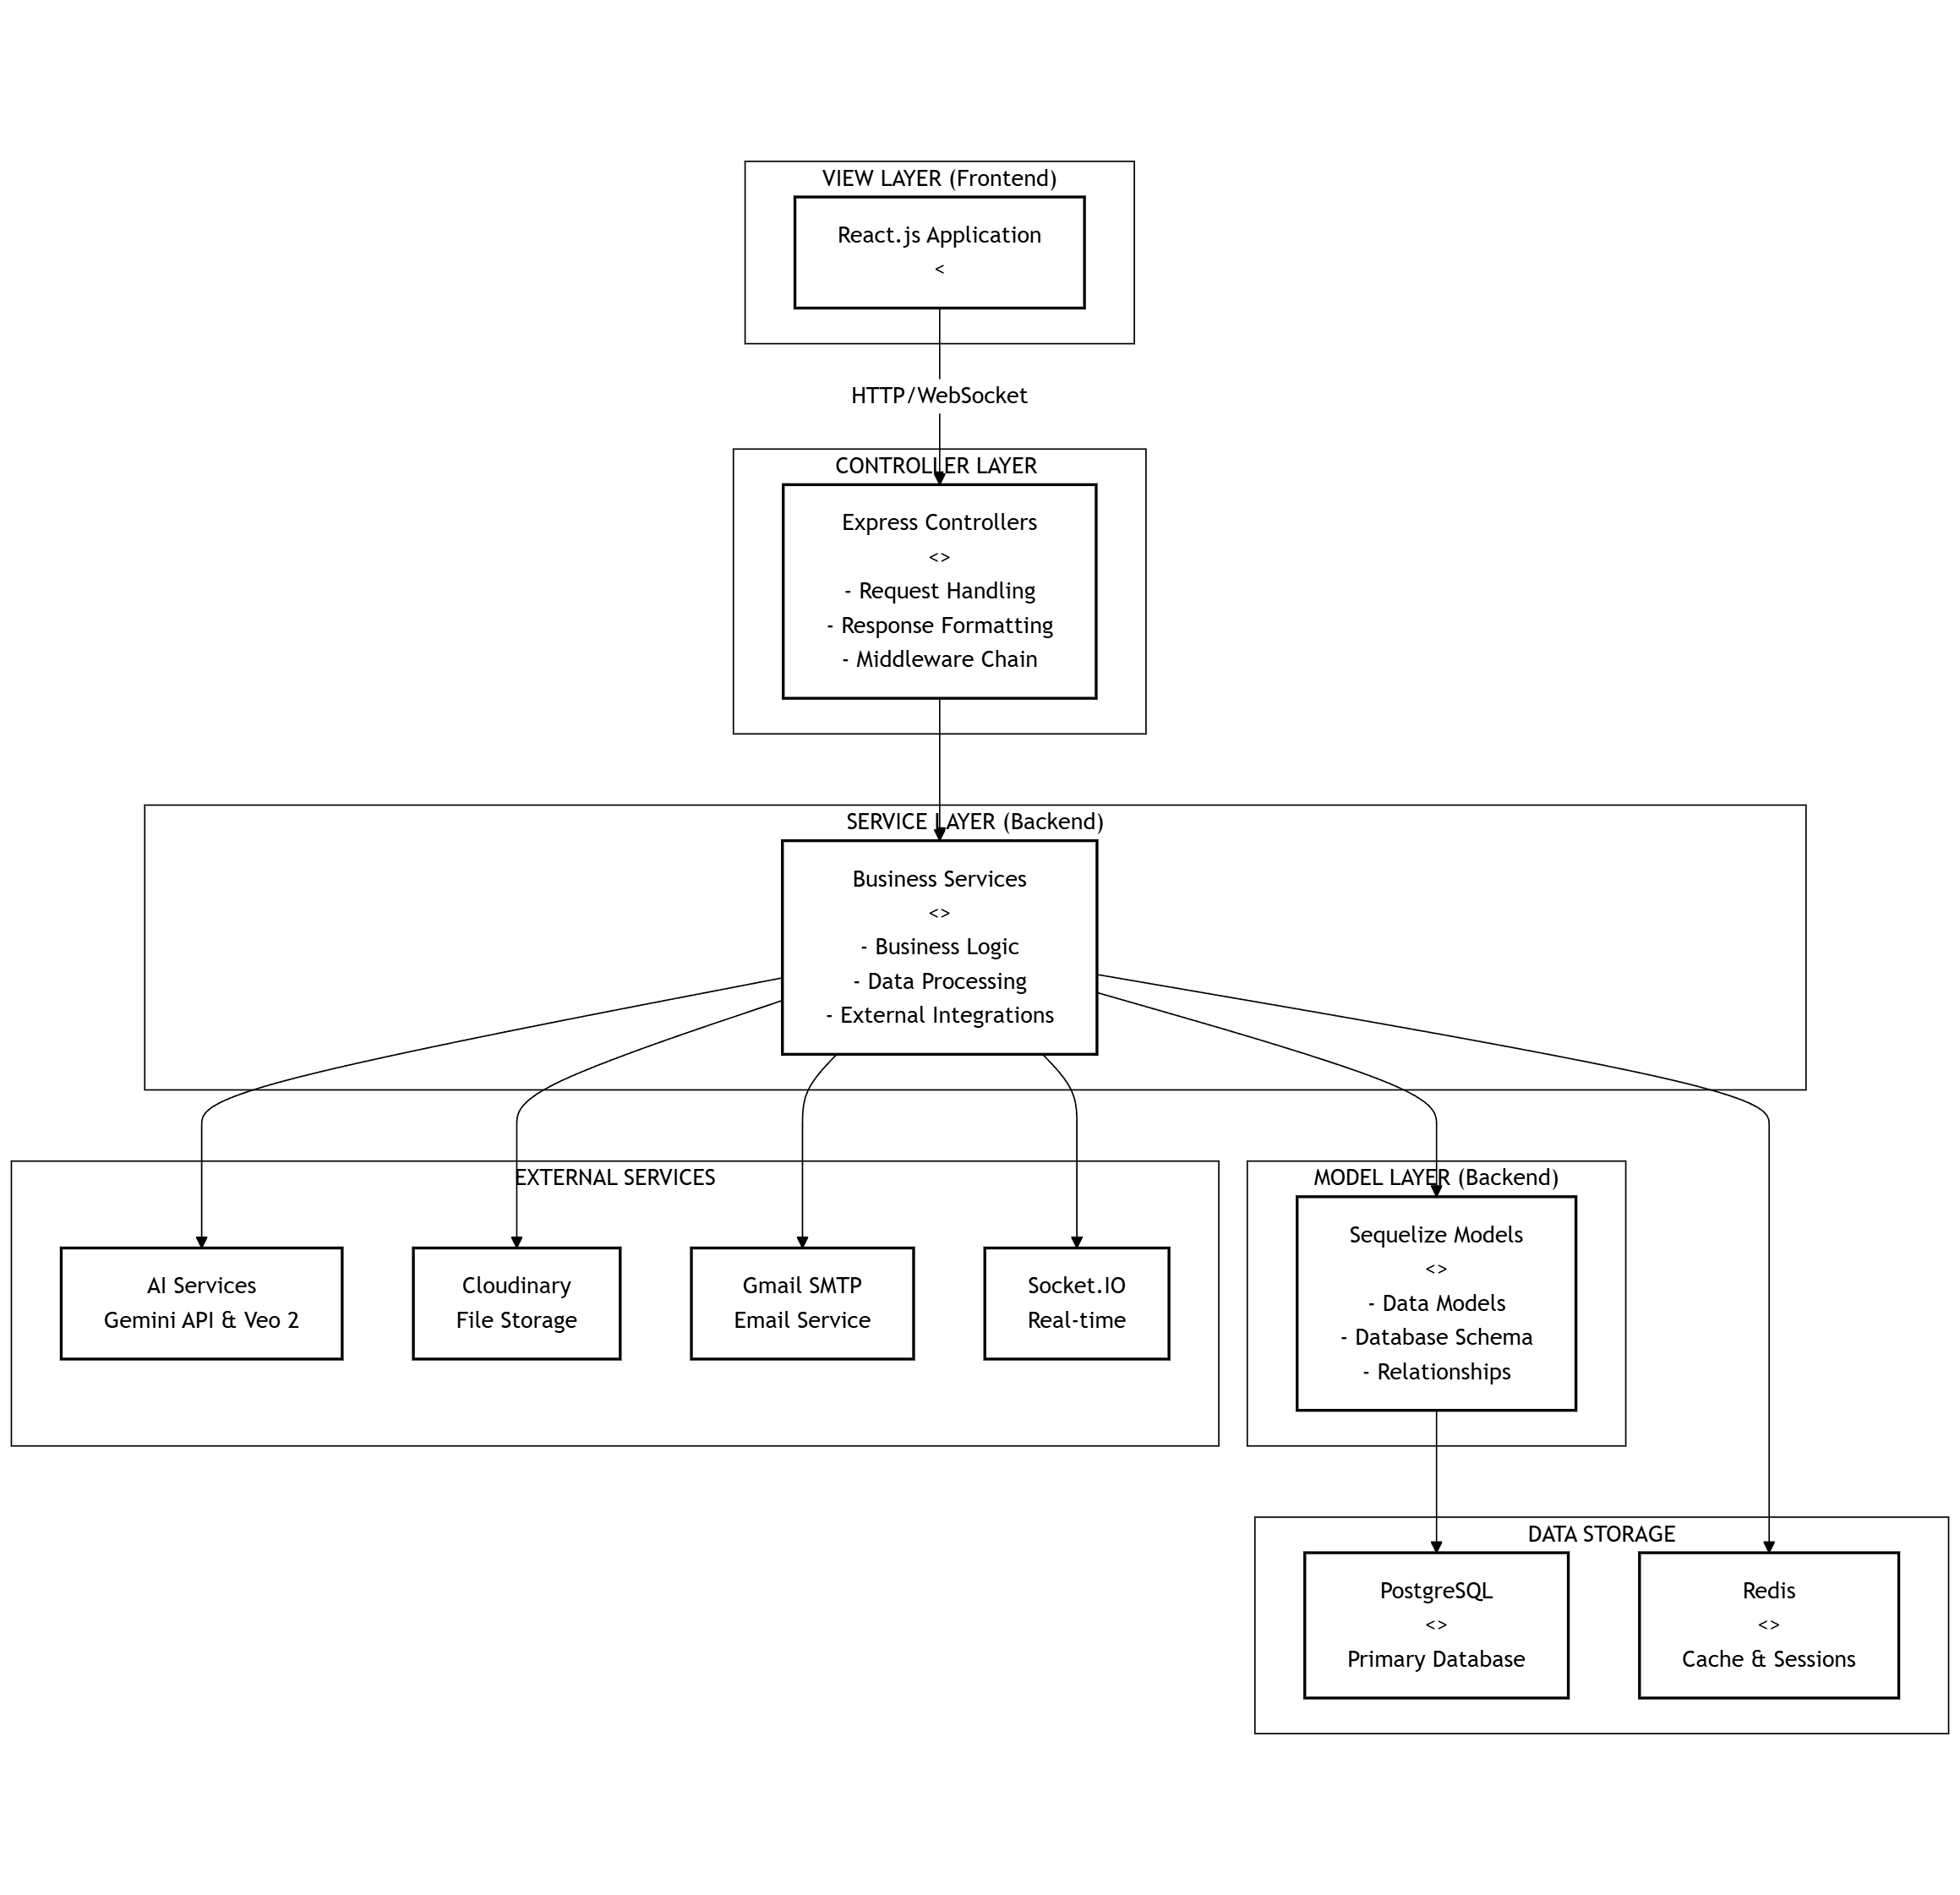
\includegraphics[width=0.9\textwidth]{Images/Component Diagrams/Component Diagram Overview.png}
    \caption{Component Diagram - Tổng quan hệ thống theo MVCS}
    \label{fig:component-overview}
\end{figure}

\paragraph{View Layer (Frontend)} \textbf{View Layer} được xây dựng bằng \textbf{React.js}, \textbf{TypeScript} và \textbf{Vite}, bao gồm:
\begin{itemize}
    \item \textbf{Main Frontend}: Ứng dụng cho buyer/seller/guest, gồm feed, marketplace, cart, checkout, orders, profile, groups, messages, notifications, AI creative lab, AI shopping assistant và seller dashboard.
    \item \textbf{Admin Frontend}: Ứng dụng riêng cho admin, gồm dashboard, users, content, reports, categories, sellers và settings.
    \item \textbf{State \& Context}: Quản lý auth state, notification state, messaging state và các state theo feature.
    \item \textbf{API Services}: Giao tiếp với backend qua REST API bằng fetch wrapper và kết nối Socket.IO cho real-time.
\end{itemize}

\paragraph{Controller Layer (Backend)} \textbf{Controller Layer} được xây dựng bằng \textbf{Express.js}, chịu trách nhiệm:
\begin{itemize}
    \item \textbf{Request Handling}: Nhận và xử lý HTTP request từ frontend.
    \item \textbf{Response Formatting}: Trả response thống nhất cho client.
    \item \textbf{Middleware Chain}: Áp dụng authentication, authorization, validation, rate limiting và error handling.
\end{itemize}

\paragraph{Service Layer (Backend)} \textbf{Service Layer} chứa business logic của hệ thống:
\begin{itemize}
    \item \textbf{Auth \& User Service}: Đăng ký, verify email, login, 2FA, reset password, profile và privacy settings.
    \item \textbf{Social Services}: Feed, posts, likes, comments, follow, saved items, groups và reports.
    \item \textbf{Commerce Services}: Products, variants, cart, orders, refunds, reviews, seller stats và product recommendations.
    \item \textbf{Realtime Services}: Messaging, notification và Socket.IO event emission.
    \item \textbf{AI Services}: Tạo nội dung text, image+text, lưu lịch sử AI, liên kết nội dung với post/scheduled post và cung cấp AI Shopping Assistant qua chatbox.
    \item \textbf{Admin Services}: Quản lý users, content, categories, seller verification và reports.
    \item \textbf{Cache Helper}: Đọc/ghi Redis cho các endpoint đọc nhiều như product list/detail, post list/detail, post comments và search; đồng thời xóa cache liên quan khi dữ liệu bài viết hoặc sản phẩm thay đổi.
\end{itemize}

\paragraph{Model/Data Access Layer (Backend)} \textbf{Model Layer} sử dụng \textbf{Prisma ORM} để:
\begin{itemize}
    \item \textbf{Data Models}: Định nghĩa schema dữ liệu tại \texttt{database/prisma/schema.prisma}.
    \item \textbf{Database Access}: Truy vấn và cập nhật PostgreSQL thông qua Prisma Client.
    \item \textbf{Relationships}: Quản lý quan hệ giữa users, products, orders, posts, groups, messages, notifications, reports và các bảng hỗ trợ.
\end{itemize}

\paragraph{Data Storage \& External Services} Hệ thống sử dụng:
\begin{itemize}
    \item \textbf{PostgreSQL}: Database chính lưu trữ dữ liệu nghiệp vụ.
    \item \textbf{Prisma Client}: Tầng ORM/data access cho backend.
    \item \textbf{Redis}: Cache tùy chọn cho dữ liệu đọc nhiều, được cấu hình bằng \texttt{REDIS\_URL}.
    \item \textbf{Cloudinary}: Lưu trữ và quản lý hình ảnh/file upload.
    \item \textbf{SMTP/Nodemailer}: Gửi email xác thực, OTP và reset password.
    \item \textbf{Socket.IO}: Giao tiếp real-time giữa frontend và core backend.
    \item \textbf{AI Providers}: Gemini cho text/vision; Hugging Face hoặc Replicate cho image generation nếu được cấu hình.
\end{itemize}

\paragraph{MVCS Flow} Luồng xử lý trong hệ thống:
\begin{enumerate}
    \item \textbf{View Layer} gửi request đến backend qua HTTP hoặc kết nối realtime qua Socket.IO.
    \item \textbf{Controller Layer} xác thực, validate và gọi service phù hợp.
    \item \textbf{Service Layer} thực hiện business logic và tương tác với Prisma Client.
    \item \textbf{Prisma Client} truy vấn hoặc cập nhật \textbf{PostgreSQL}.
    \item Với các endpoint đọc nhiều, \textbf{Controller/Cache Helper} có thể lấy dữ liệu từ \textbf{Redis} trước khi gọi service; khi có thay đổi dữ liệu, cache liên quan được invalidation theo pattern.
    \item \textbf{Service Layer} có thể gọi \textbf{Cloudinary}, \textbf{SMTP} hoặc \textbf{AI Providers} khi cần.
    \item Kết quả được trả về frontend; các sự kiện realtime được emit qua Socket.IO.
\end{enumerate}

\subsubsection{Component diagram theo vai trò người dùng}

Để dễ hiểu và phát triển các tính năng cụ thể, chúng tôi chia component diagram thành các diagram theo từng vai trò người dùng trong hệ thống.

\paragraph{Component diagram cho User/Buyer} \ref{fig:component-user-buyer} mô tả các components và flow dành cho người dùng thông thường (User/Buyer).

\begin{figure}[htbp]
    \centering
    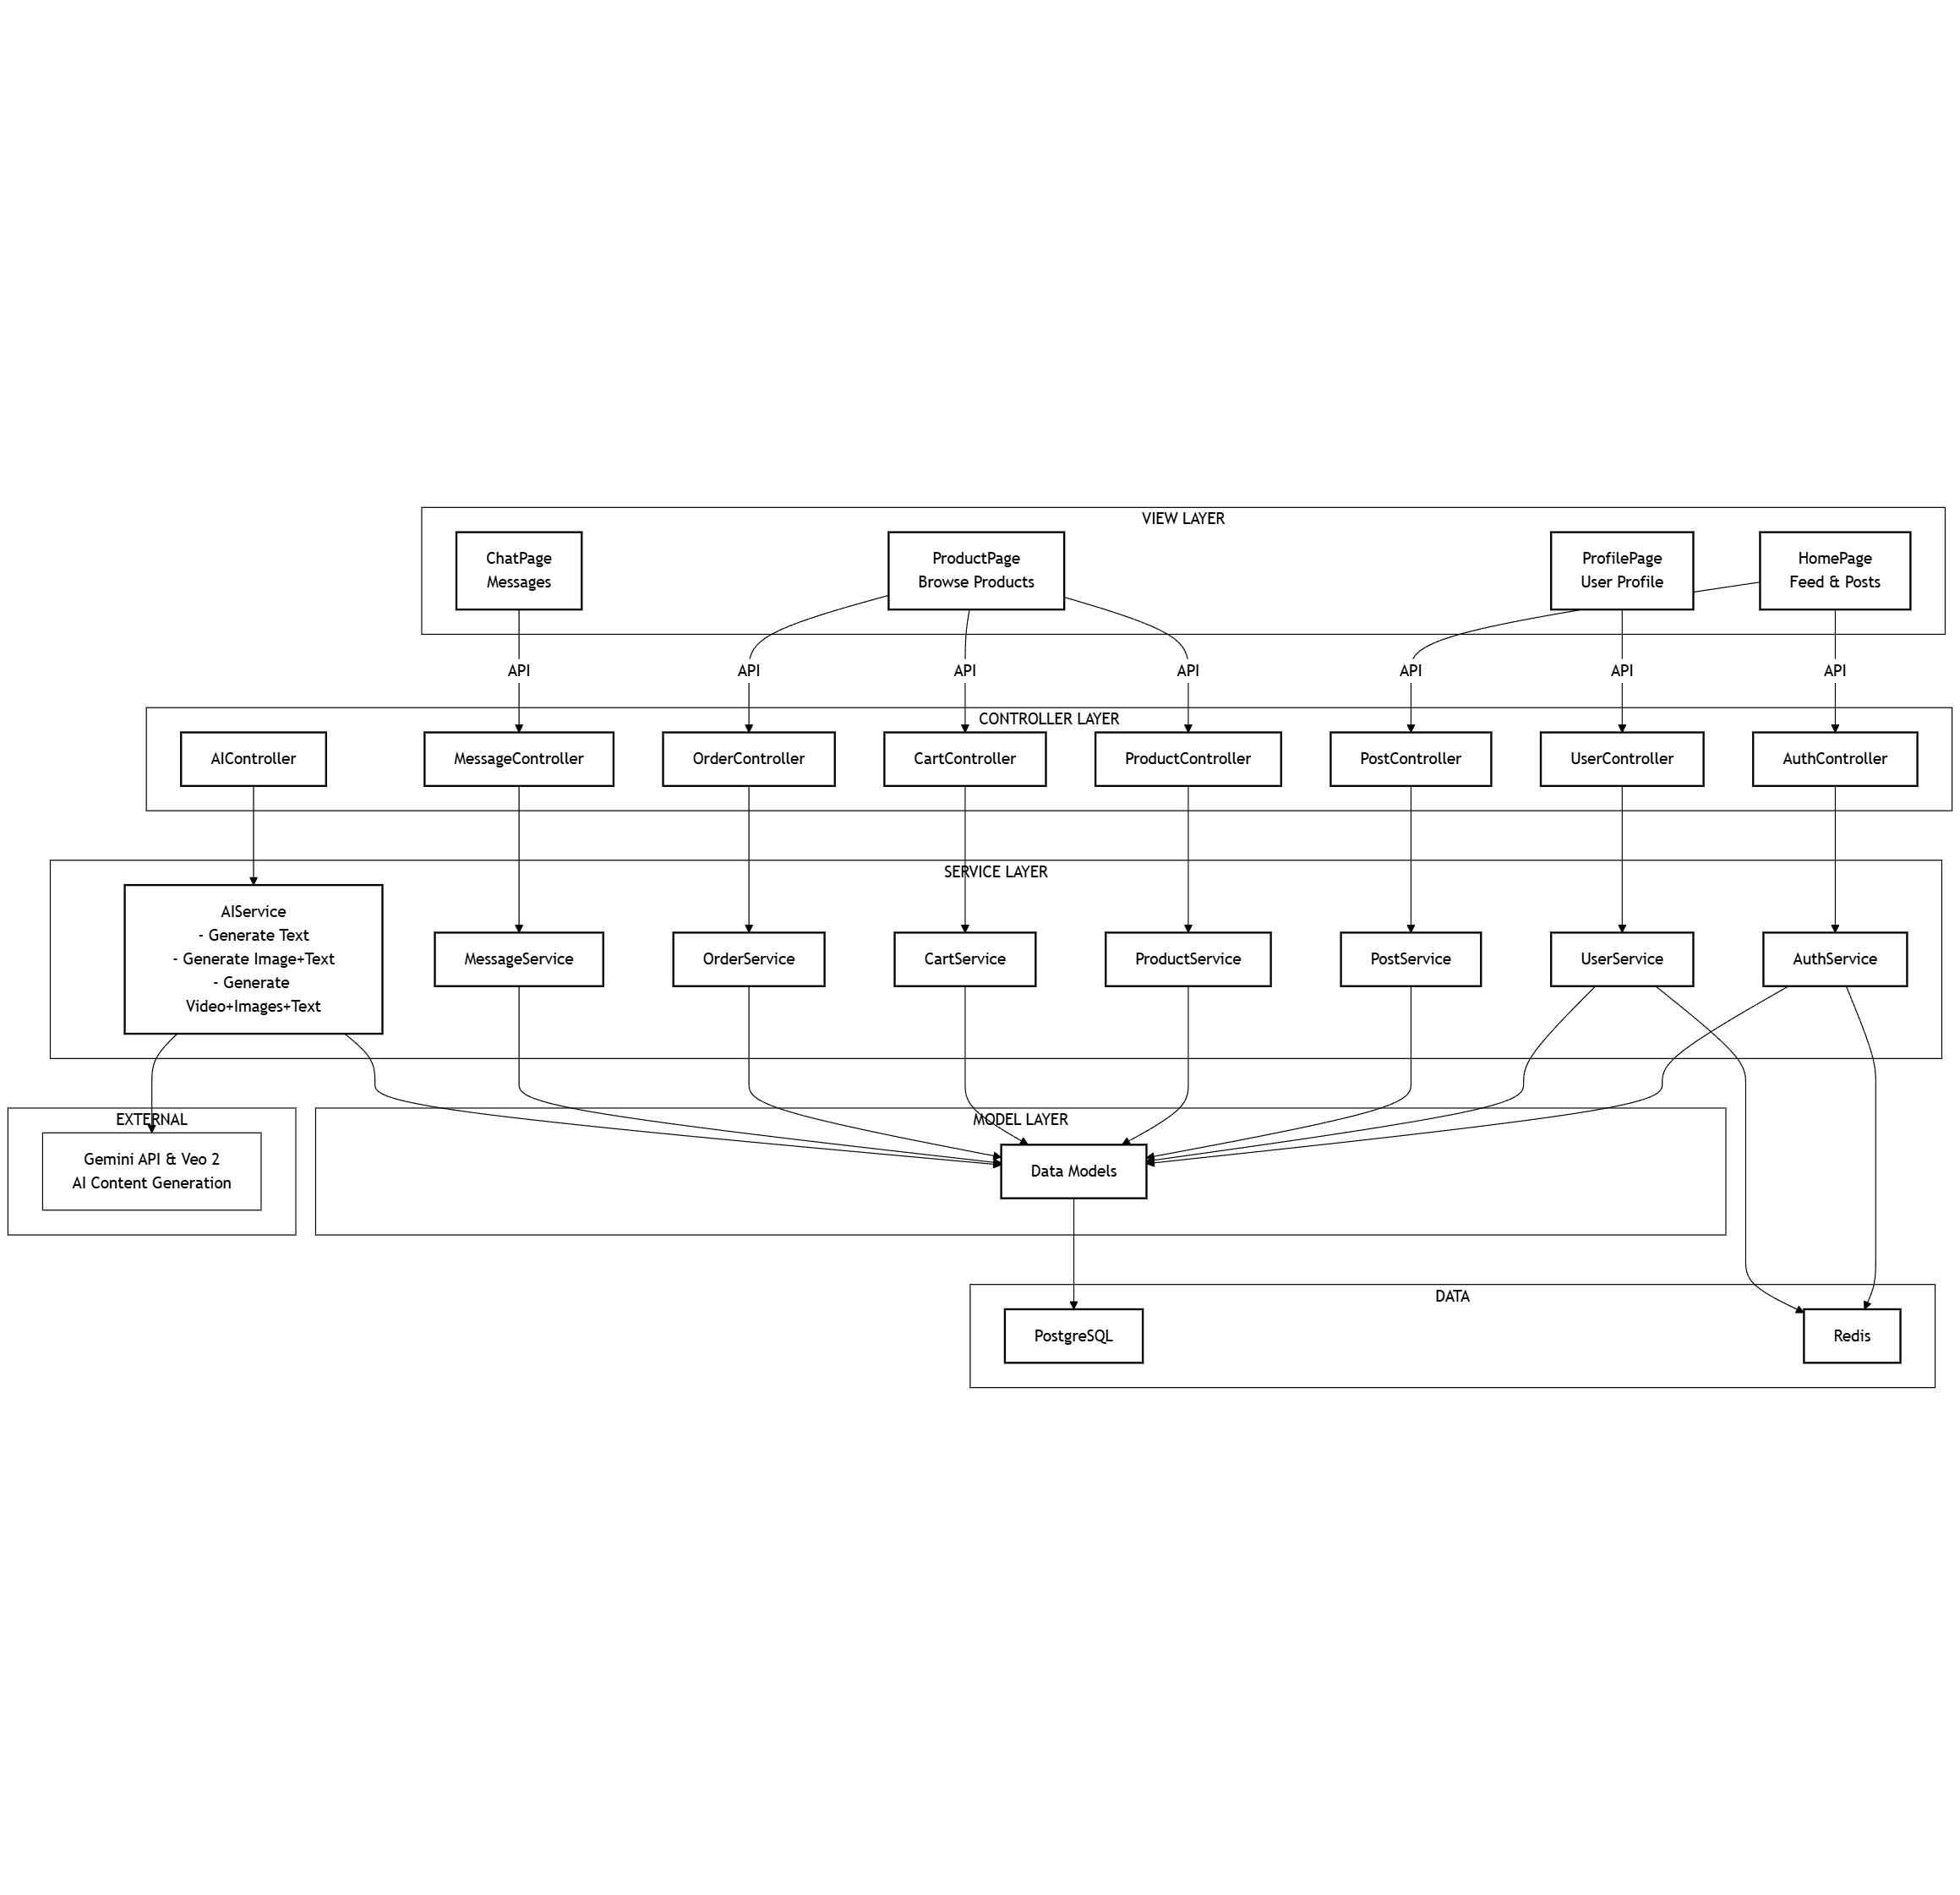
\includegraphics[width=0.9\textwidth]{Images/Component Diagrams/UserBuyer Component Diagram.png}
    \caption{Component Diagram - User/Buyer Role}
    \label{fig:component-user-buyer}
\end{figure}

\textbf{View Layer} bao gồm các trang:
\begin{itemize}
    \item \textbf{Feed/Home}: Trang feed, bài viết và tương tác xã hội.
    \item \textbf{Marketplace/Product Detail}: Duyệt, tìm kiếm, lọc và xem sản phẩm.
    \item \textbf{Cart/Checkout/Orders}: Giỏ hàng, đặt hàng, xác nhận thanh toán và theo dõi đơn.
    \item \textbf{Profile/Saved Items}: Hồ sơ, follow và danh sách đã lưu.
    \item \textbf{Groups/Messages/Notifications}: Nhóm cộng đồng, nhắn tin và thông báo.
\end{itemize}

\textbf{Controller Layer} xử lý các request từ frontend:
\begin{itemize}
    \item \textbf{AuthController, UserController}: Xác thực, profile, follow.
    \item \textbf{PostController, GroupController, ReportController}: Bài viết, nhóm, tương tác và báo cáo.
    \item \textbf{ProductController, CartController, OrderController, ReviewController}: Marketplace, giỏ hàng, đơn hàng và đánh giá.
    \item \textbf{MessageController, NotificationController}: Tin nhắn và thông báo realtime.
\end{itemize}

\textbf{Service Layer} thực hiện business logic tương ứng, còn \textbf{Model Layer} truy cập dữ liệu qua Prisma và PostgreSQL.

\paragraph{Component diagram cho Seller} \ref{fig:component-seller} mô tả các components và flow dành cho người bán (Seller).

\begin{figure}[htbp]
    \centering
    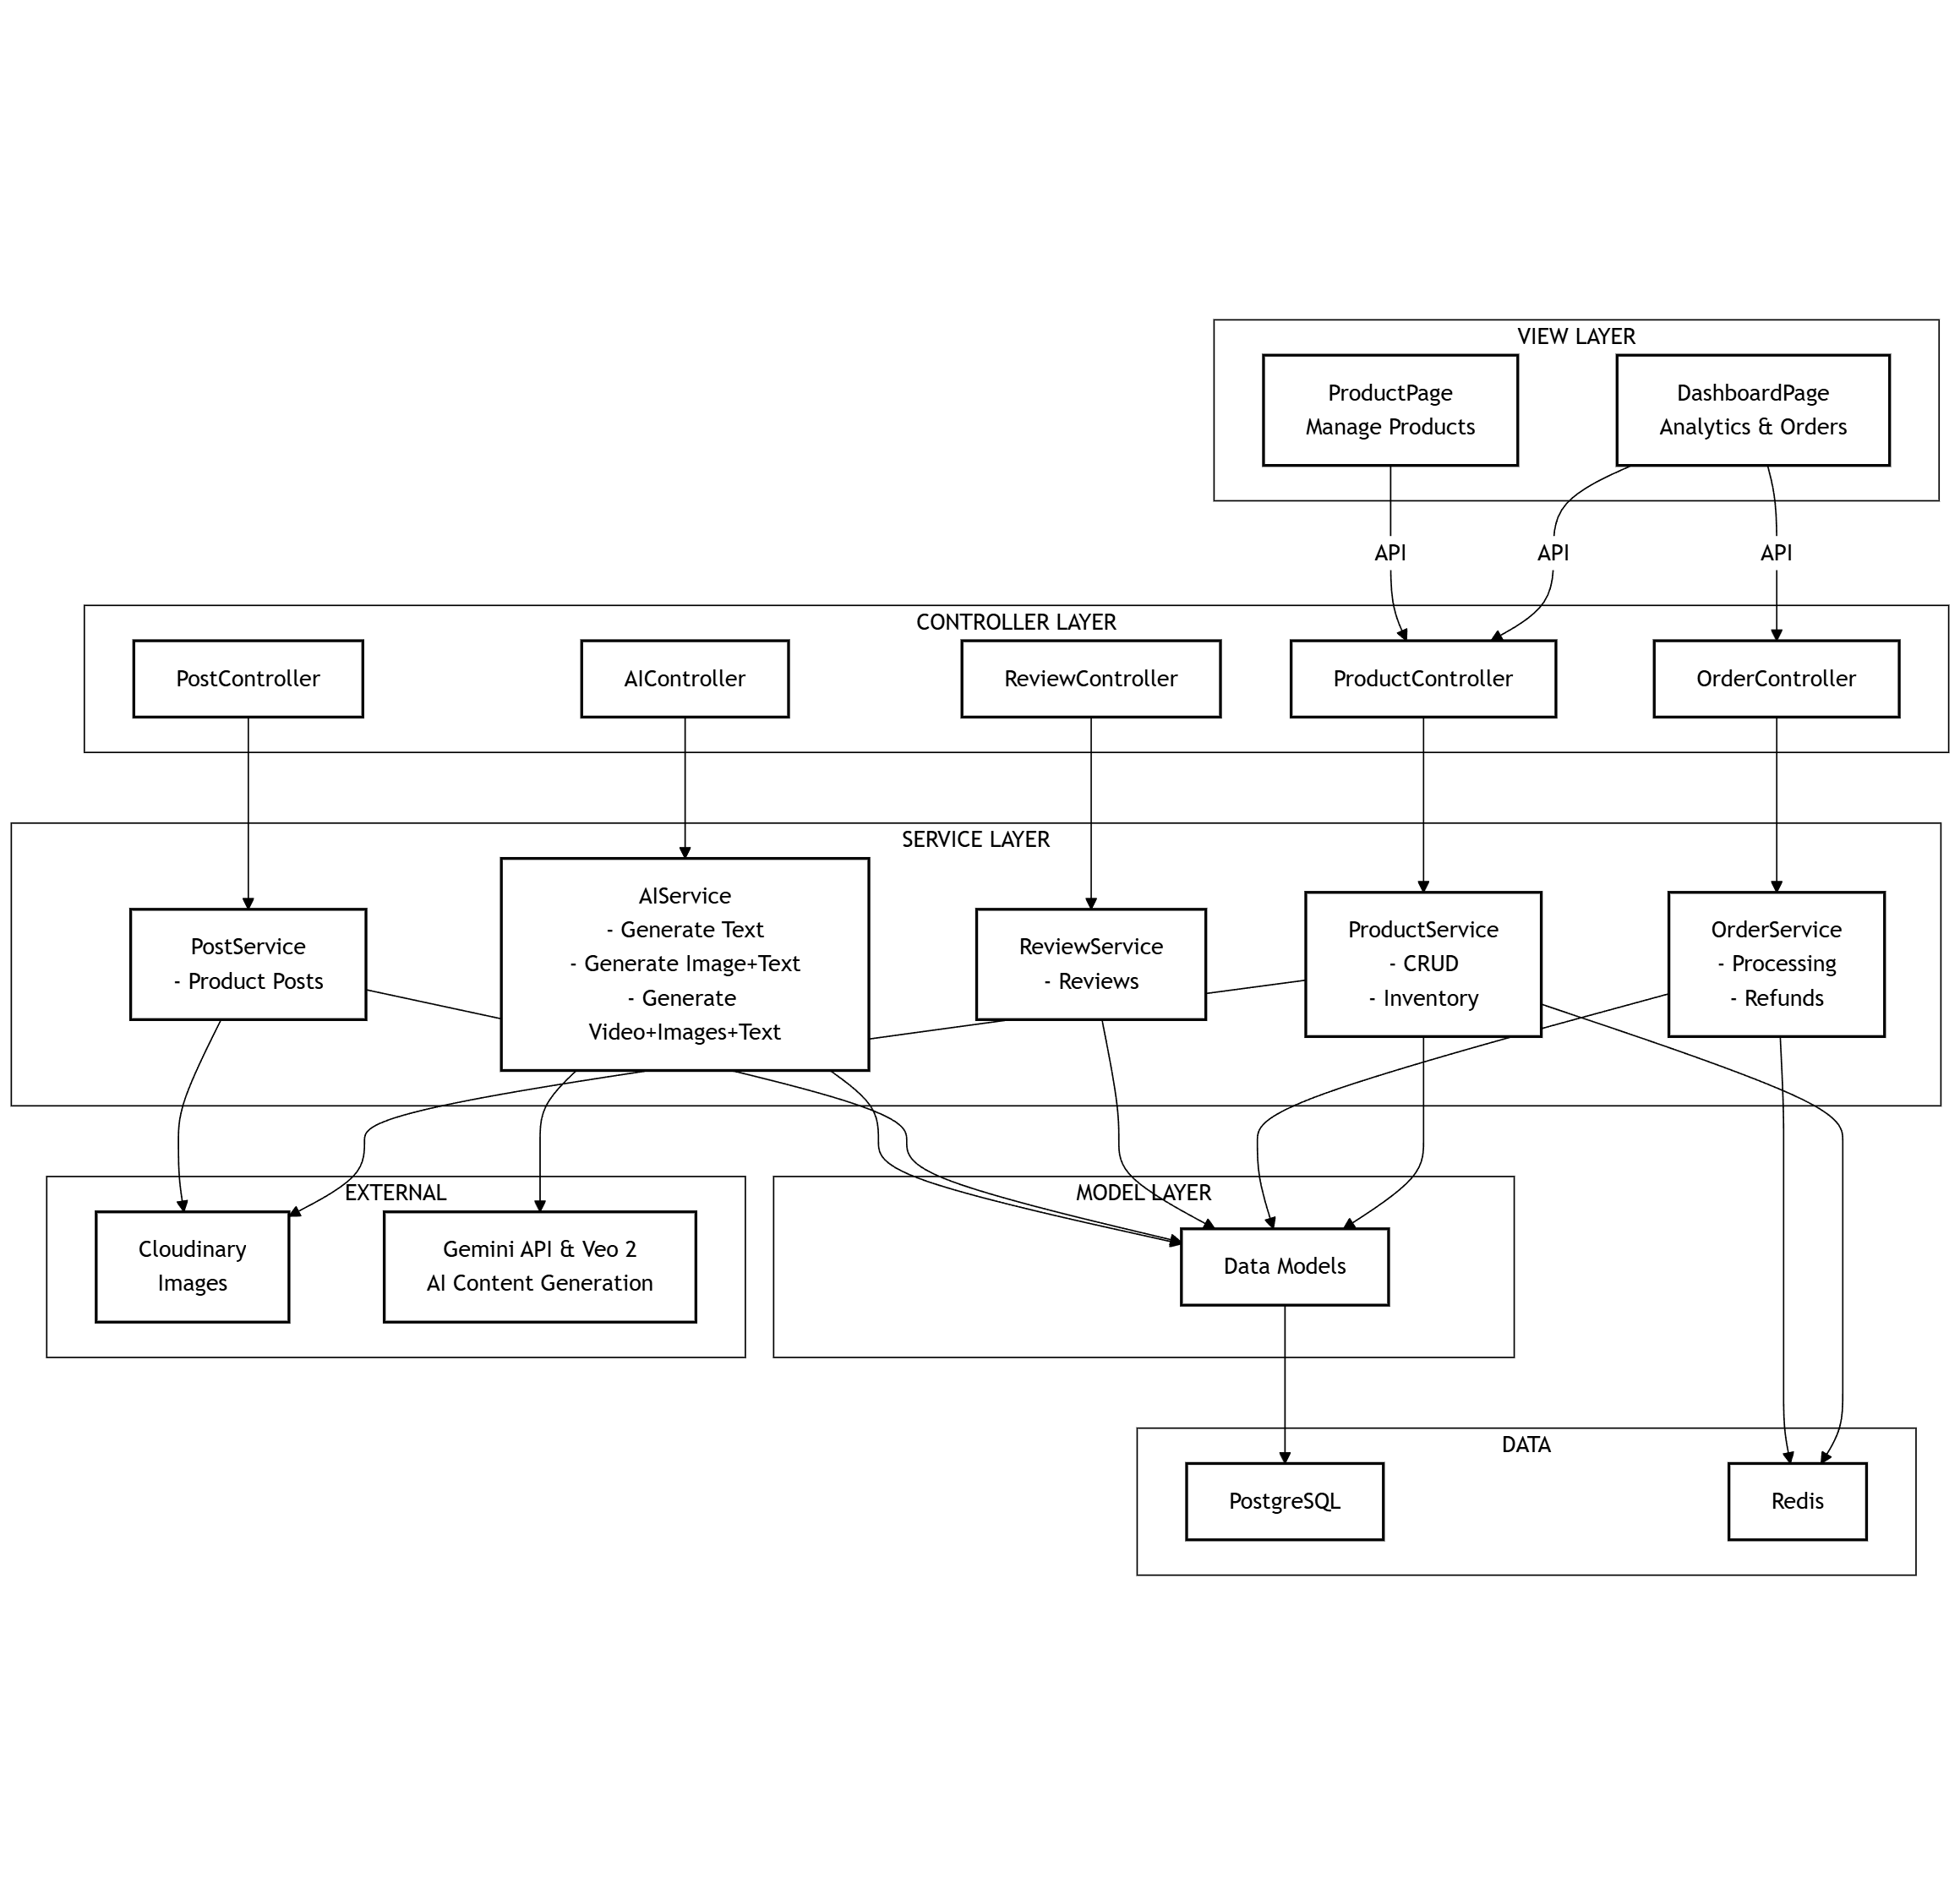
\includegraphics[width=0.9\textwidth]{Images/Component Diagrams/Seller Component Diagram.png}
    \caption{Component Diagram - Seller Role}
    \label{fig:component-seller}
\end{figure}

\textbf{View Layer} cho Seller bao gồm:
\begin{itemize}
    \item \textbf{Seller Registration}: Quy trình đăng ký seller nhiều bước, upload giấy tờ và theo dõi trạng thái duyệt.
    \item \textbf{Seller Dashboard}: Tổng quan doanh thu, đơn hàng, lượt xem và tồn kho.
    \item \textbf{Products/Inventory}: Quản lý sản phẩm, ảnh, biến thể, trạng thái và soft delete/restore.
    \item \textbf{Orders/Refunds/Reviews}: Quản lý đơn bán, xử lý hoàn tiền và phản hồi đánh giá.
    \item \textbf{Scheduled Posts/AI Lab}: Lên lịch bài đăng, tạo nội dung bằng AI và tư vấn mua sắm qua AI chatbox.
\end{itemize}

\textbf{Controller Layer} xử lý các chức năng của Seller:
\begin{itemize}
    \item \textbf{SellerController}: Đăng ký seller, xác minh hồ sơ, sensitive re-auth và change request.
    \item \textbf{ProductController}: Quản lý sản phẩm, inventory và variants.
    \item \textbf{OrderController}: Xem/cập nhật trạng thái đơn hàng và xử lý hoàn tiền.
    \item \textbf{ReviewController}: Phản hồi đánh giá.
    \item \textbf{ScheduledPostController}: CRUD bài đăng đã lên lịch và publish ngay.
    \item \textbf{AIController/AiAssistantController}: Tạo nội dung AI, quản lý lịch sử và xử lý chatbox tư vấn mua sắm.
\end{itemize}

Seller sử dụng \textbf{Cloudinary} để upload ảnh sản phẩm, shop logo/cover và giấy tờ xác minh.

\paragraph{Component diagram cho Admin} \ref{fig:component-admin} mô tả các components và flow dành cho quản trị viên (Admin).

\begin{figure}[htbp]
    \centering
    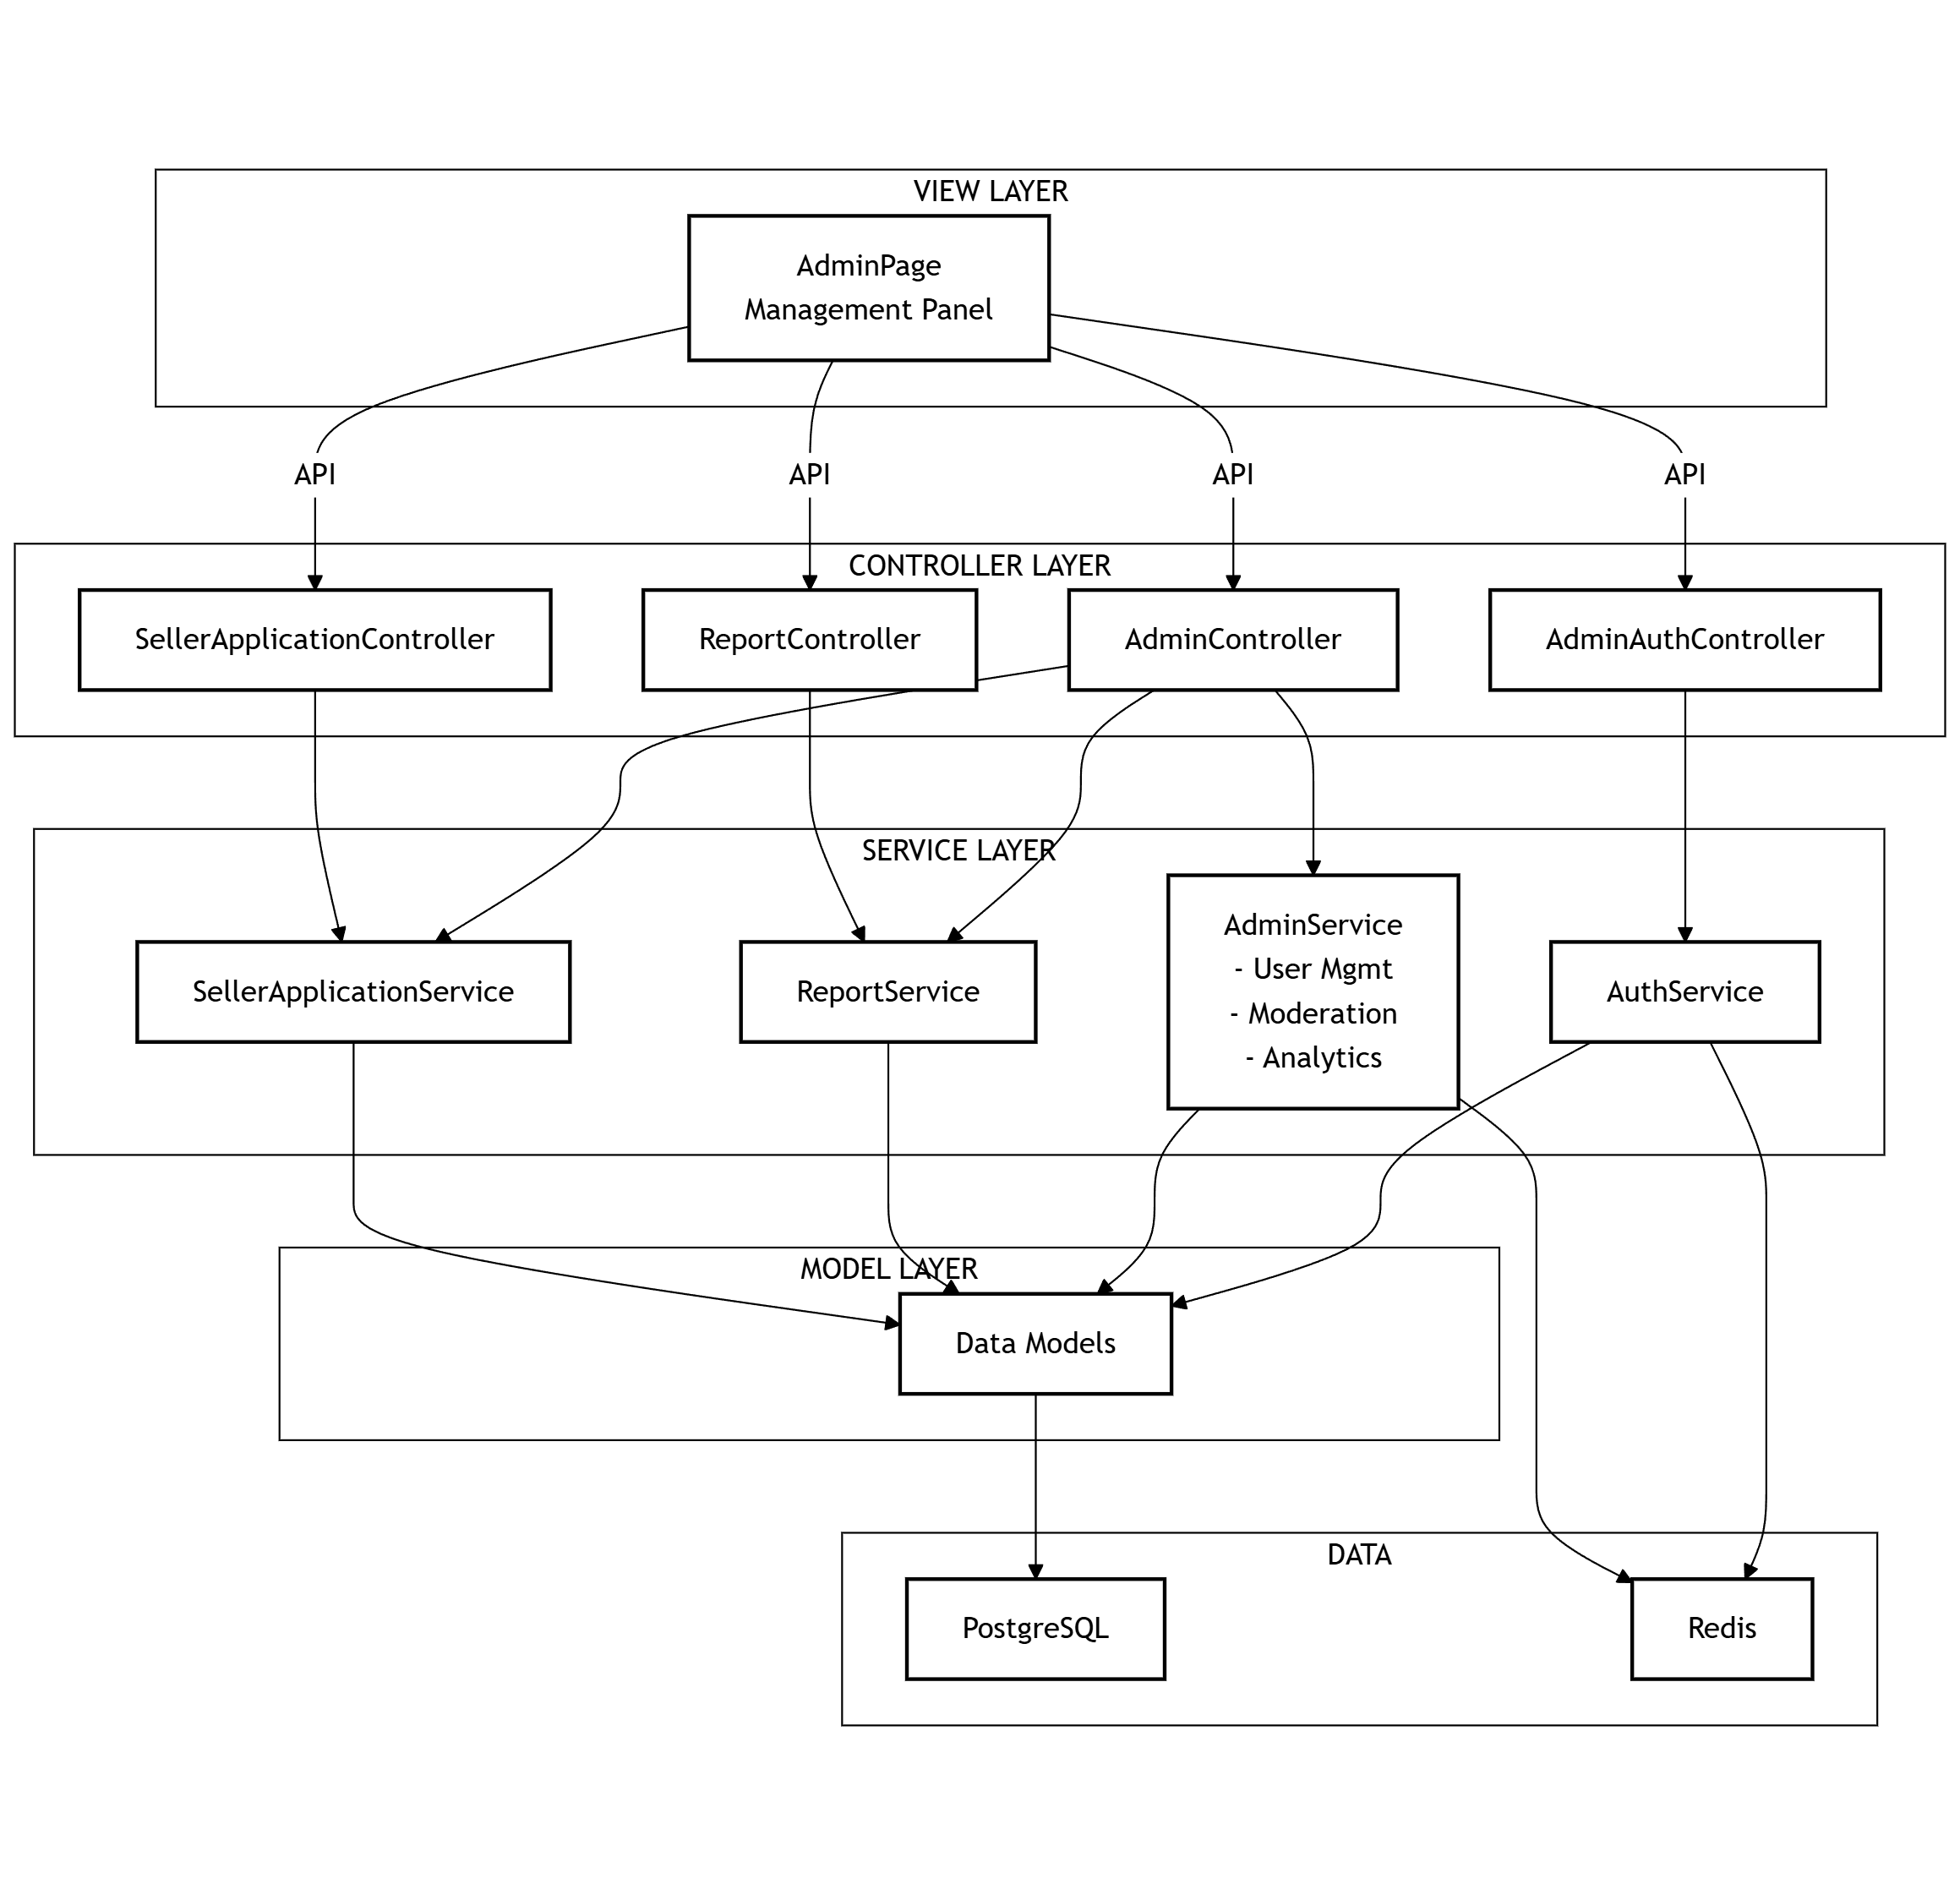
\includegraphics[width=0.9\textwidth]{Images/Component Diagrams/Admin Component Diagram.png}
    \caption{Component Diagram - Admin Role}
    \label{fig:component-admin}
\end{figure}

\textbf{View Layer} cho Admin bao gồm:
\begin{itemize}
    \item \textbf{Admin Login}: Đăng nhập admin qua admin API.
    \item \textbf{Dashboard}: Thống kê tổng quan và growth.
    \item \textbf{Users}: Quản lý user, trạng thái active và role.
    \item \textbf{Content}: Quản lý bài viết và sản phẩm.
    \item \textbf{Reports}: Xem và xử lý báo cáo vi phạm.
    \item \textbf{Categories}: Quản lý danh mục.
    \item \textbf{Sellers}: Duyệt hồ sơ seller và yêu cầu thay đổi dữ liệu nhạy cảm.
\end{itemize}

\textbf{Controller/Service Layer} cho Admin bao gồm:
\begin{itemize}
    \item \textbf{AdminAuthController/AuthService}: Xác thực admin.
    \item \textbf{AdminController/AdminService}: Users, content, categories và dashboard.
    \item \textbf{ReportController/ReportService}: Reports và moderation actions.
    \item \textbf{SellerAdmin Routes/SellerController}: Seller applications và sensitive change requests.
\end{itemize}

\paragraph{Lợi ích của việc chia nhỏ component diagram} Việc chia component diagram thành tổng quan và theo từng vai trò mang lại các lợi ích:
\begin{itemize}
    \item \textbf{Dễ hiểu}: Mỗi diagram tập trung vào một mục đích cụ thể.
    \item \textbf{Dễ maintain}: Cập nhật dễ hơn khi một module thay đổi.
    \item \textbf{Dễ phát triển}: Developers có thể tập trung vào diagram liên quan đến feature đang làm.
    \item \textbf{Dễ tài liệu hóa}: Tài liệu rõ ràng hơn cho từng user type và nhóm chức năng.
\end{itemize}


\section{Deployment Diagram}
Deployment diagram mô tả kiến trúc triển khai (deployment architecture) của hệ thống Social Commerce, bao gồm các thành phần phần cứng, phần mềm, môi trường triển khai và các kết nối giữa chúng. Diagram này giúp hiểu rõ cách hệ thống được triển khai trên môi trường production và cách các thành phần tương tác với nhau.

\subsection{Tổng quan kiến trúc triển khai}

\ref{fig:deployment-diagram} mô tả kiến trúc triển khai tổng thể của hệ thống, bao gồm các layers chính: Client Layer, CDN Layer, Application Server, Database và External Services.

\begin{figure}[htbp]
    \centering
    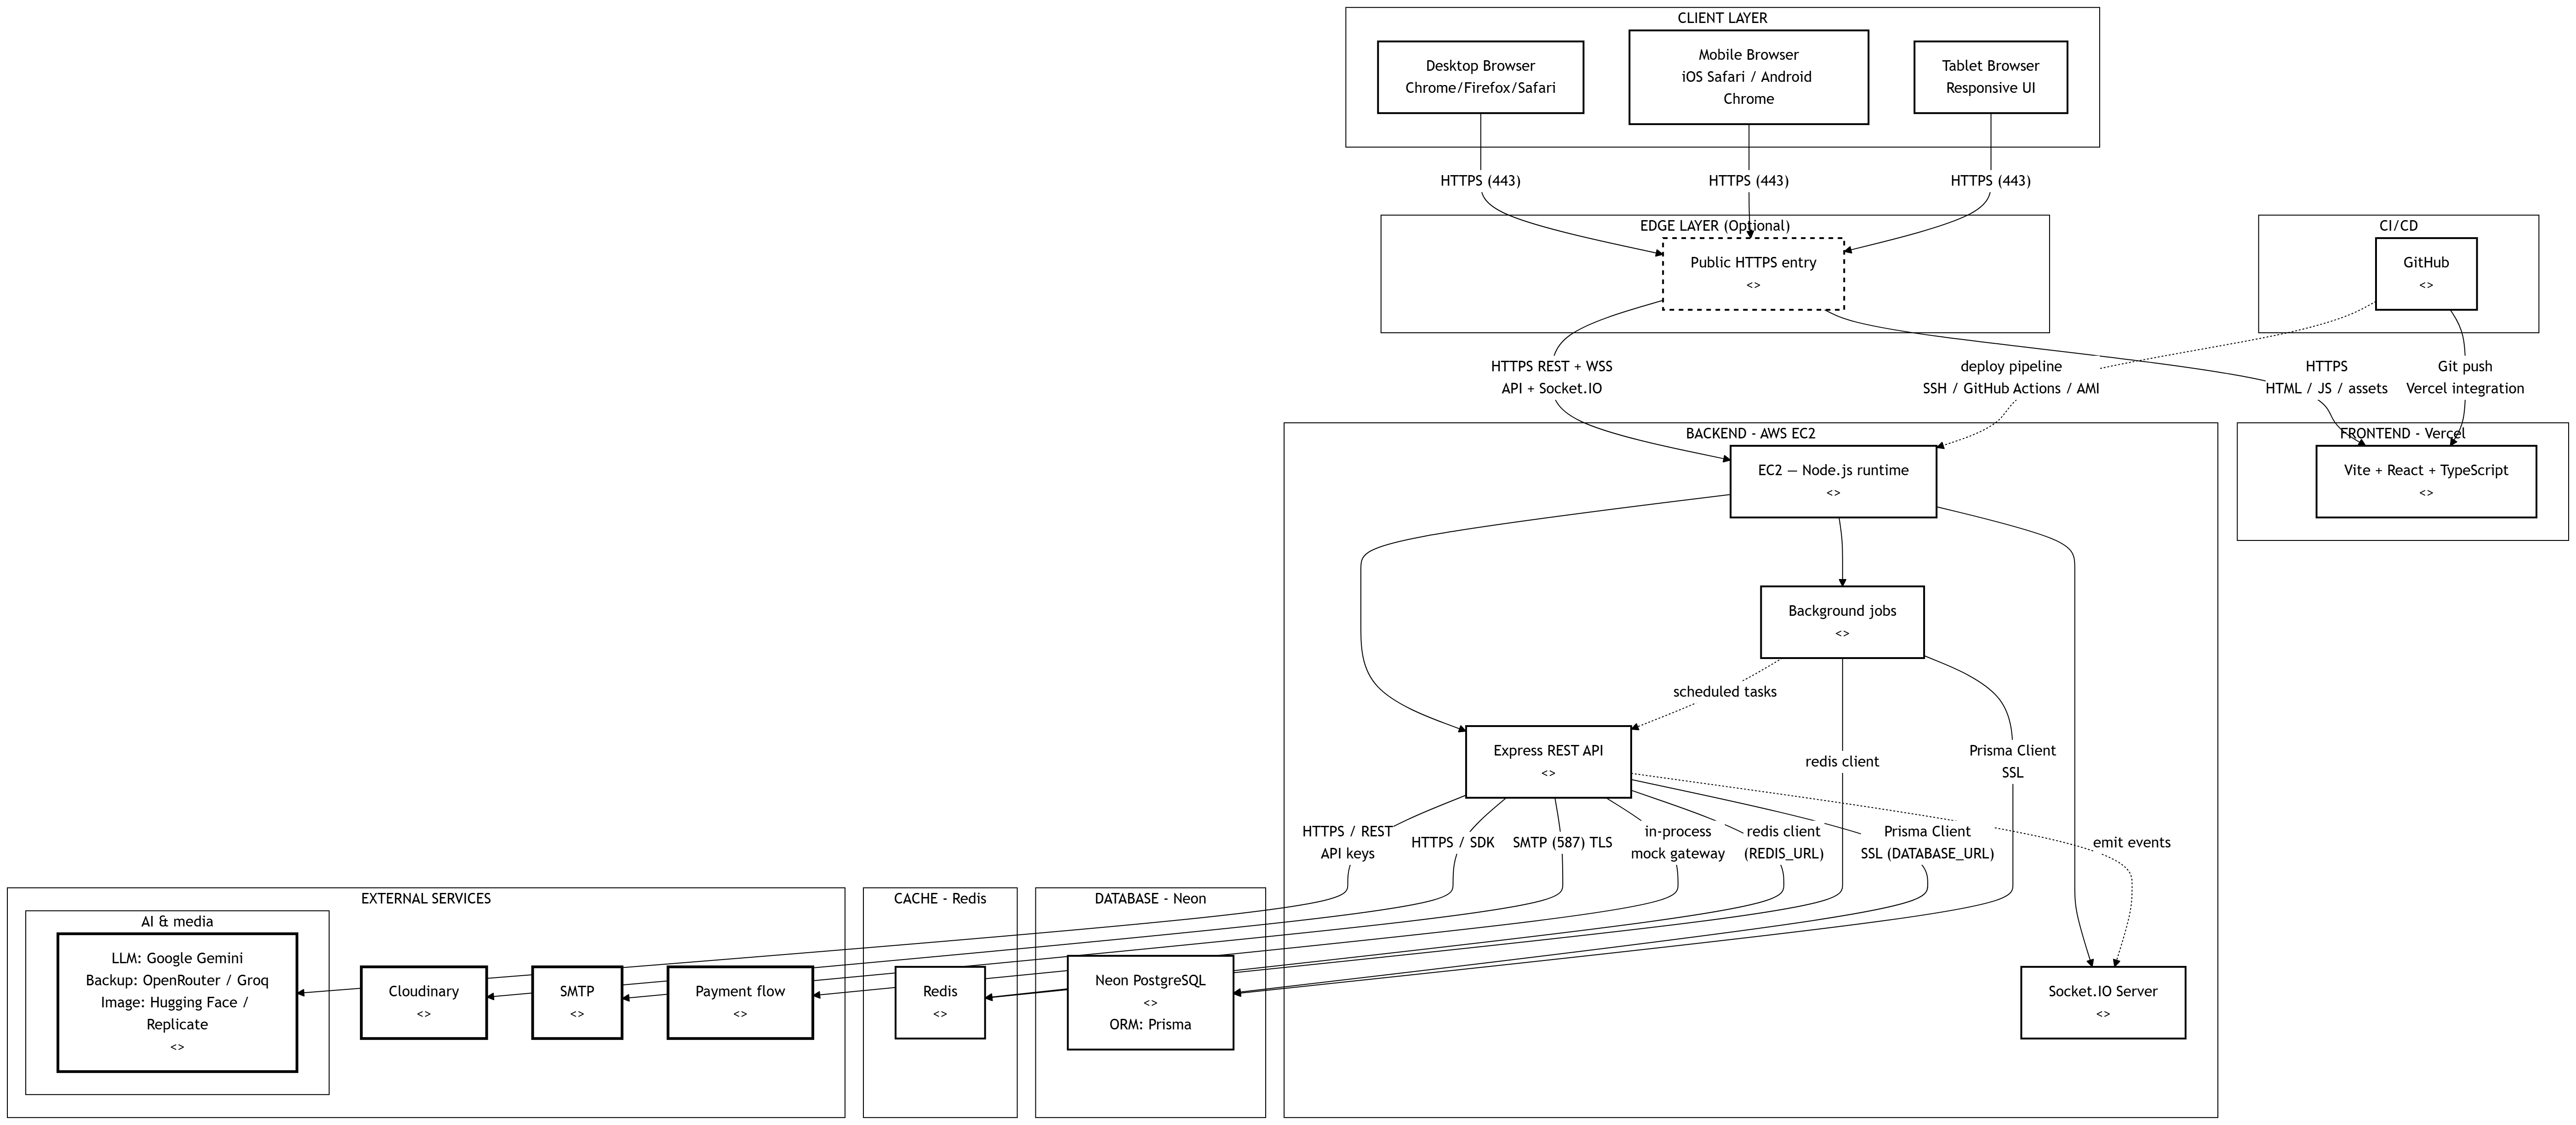
\includegraphics[width=\textwidth]{Images/Deployment Diagram.png}
    \caption{Deployment Diagram - Kiến trúc triển khai hệ thống}
    \label{fig:deployment-diagram}
\end{figure}

\subsection{Các thành phần chính}

\subsubsection{Client Layer}

\textbf{Client Layer} bao gồm các thiết bị và trình duyệt mà người dùng sử dụng để truy cập hệ thống:

\begin{itemize}
    \item \textbf{Desktop Browser}: Chrome, Firefox, Safari trên máy tính
    \item \textbf{Mobile Browser}: iOS Safari, Android Chrome trên điện thoại di động
    \item \textbf{Tablet Browser}: Giao diện responsive trên máy tính bảng
\end{itemize}

Tất cả các client kết nối đến hệ thống thông qua giao thức \textbf{HTTPS (port 443)} cho các request thông thường và \textbf{WebSocket Secure (WSS)} cho các tính năng real-time như thông báo và chat.

\subsubsection{CDN Layer (Optional)}

\textbf{Cloudflare CDN} là tầng tùy chọn được sử dụng để:

\begin{itemize}
    \item \textbf{Caching}: Lưu cache các static assets (HTML, CSS, JavaScript, images) để tăng tốc độ tải trang
    \item \textbf{DDoS Protection}: Bảo vệ hệ thống khỏi các cuộc tấn công DDoS
    \item \textbf{SSL/TLS Termination}: Xử lý chứng chỉ SSL/TLS, giảm tải cho application server
\end{itemize}

Khi CDN được triển khai, các static files sẽ được phục vụ từ CDN (cache hit), trong khi các request động sẽ được chuyển tiếp đến application server (cache miss). WebSocket connections có thể bypass CDN để kết nối trực tiếp với application server để đảm bảo độ trễ thấp.

\subsubsection{Application Server}

Hệ thống được triển khai trên \textbf{Render.com}, một platform-as-a-service (PaaS) cloud, với các thành phần sau:

\paragraph{Node.js Runtime} 
Môi trường thực thi sử dụng \textbf{Node.js version >= 18.0.0}, cung cấp nền tảng để chạy ứng dụng backend.

\paragraph{React Frontend}
Frontend được build bằng \textbf{Vite} và được deploy dưới dạng static files. Trong production, Express server phục vụ các static files này từ thư mục \texttt{frontend/dist/}, bao gồm:
\begin{itemize}
    \item HTML files
    \item JavaScript bundles
    \item CSS stylesheets
    \item Assets (images, fonts, etc.)
\end{itemize}

\paragraph{Express API Server}
Backend được xây dựng bằng \textbf{Express.js framework}, chịu trách nhiệm:
\begin{itemize}
    \item Xử lý các REST API endpoints
    \item Áp dụng middleware stack (authentication, validation, rate limiting, error handling)
    \item Thực thi business logic thông qua controllers
    \item Tích hợp với các external services
\end{itemize}

\paragraph{Socket.IO Server}
\textbf{Socket.IO server} được tích hợp vào cùng application server, cung cấp:
\begin{itemize}
    \item \textbf{WebSocket connections}: Kết nối real-time hai chiều với clients
    \item \textbf{Real-time events}: Gửi và nhận events real-time
    \item \textbf{Chat rooms}: Quản lý các phòng chat
    \item \textbf{Push Notifications}: Gửi thông báo tức thì đến clients
    \item \textbf{Live Updates}: Cập nhật trạng thái real-time (order status, notifications, etc.)
\end{itemize}

Socket.IO server tương tác với Express server để emit events khi có các thay đổi trong hệ thống (ví dụ: khi có đơn hàng mới, notification mới).

\paragraph{Background Jobs}
Hệ thống sử dụng \textbf{node-cron} để chạy các background jobs theo lịch:
\begin{itemize}
    \item \textbf{Auto-publish scheduled posts}: Tự động publish các bài viết đã được lên lịch
    \item \textbf{Cleanup old notifications}: Xóa các thông báo cũ
    \item \textbf{Reset monthly AI usage}: Reset số lần sử dụng AI theo tháng
    \item \textbf{Clean expired content requests}: Xóa các yêu cầu tạo nội dung AI đã hết hạn
\end{itemize}

Các cron jobs được chạy in-process trong cùng application server, không cần infrastructure riêng biệt.

\subsubsection{Database - PostgreSQL}

Hệ thống sử dụng \textbf{PostgreSQL} làm database chính:

\begin{itemize}
    \item \textbf{Managed Database}: Database được quản lý bởi Render.com hoặc cloud provider khác
    \item \textbf{ORM: Sequelize}: Sử dụng Sequelize ORM để tương tác với database, cung cấp abstraction layer và hỗ trợ migrations
    \item \textbf{SSL/TLS Connection}: Tất cả các kết nối đến database đều được mã hóa bằng SSL/TLS để đảm bảo bảo mật
\end{itemize}

Express server và cron jobs đều kết nối đến PostgreSQL thông qua Sequelize ORM để thực hiện các thao tác CRUD và query dữ liệu.

\subsubsection{External Services}

Hệ thống tích hợp với các external services để cung cấp các tính năng bổ sung:

\paragraph{AI Services}
\textbf{Google Gemini API và Google Veo 2} được sử dụng để:
\begin{itemize}
    \item Tạo bài viết từ mô tả, ý tưởng và hình ảnh sản phẩm (Generate Text)
    \item Tạo đồng thời bài viết và hình ảnh từ mô tả, ý tưởng và hình ảnh đầu vào (Generate Image + Text)
    \item Tạo video ngắn kèm tối đa 3 hình ảnh và bài viết từ mô tả, ý tưởng và hình ảnh đầu vào (Generate Video + Images + Text)
\end{itemize}

Kết nối đến Gemini API và Veo 2 sử dụng HTTPS/REST với API Key authentication. Hệ thống quản lý usage limit cho từng người dùng để kiểm soát chi phí và tài nguyên.

\paragraph{File Storage}
\textbf{Cloudinary} được sử dụng để:
\begin{itemize}
    \item Lưu trữ và quản lý hình ảnh, video
    \item Tối ưu hóa hình ảnh (resize, compress, format conversion)
    \item Cung cấp CDN global để phân phối assets nhanh chóng
\end{itemize}

Kết nối đến Cloudinary sử dụng HTTPS/REST API để upload và quản lý files.

\paragraph{Email Service}
\textbf{Gmail SMTP} được sử dụng để:
\begin{itemize}
    \item Gửi email thông báo đến người dùng
    \item Gửi email xác nhận đơn đăng ký seller
    \item Gửi email thông báo về đơn hàng, reviews, etc.
\end{itemize}

Kết nối sử dụng SMTP protocol (port 587) với TLS encryption, thông qua Nodemailer library.

\paragraph{Payment Simulator}
\textbf{Payment Simulator} là một mock service chạy local trong application server:
\begin{itemize}
    \item Mô phỏng quá trình thanh toán (success/failure)
    \item Chỉ sử dụng cho development và testing
    \item Không có kết nối mạng ngoài, không xử lý tiền thật
\end{itemize}

\subsubsection{CI/CD Pipeline}

\textbf{GitHub} được sử dụng làm repository để:
\begin{itemize}
    \item Lưu trữ source code
    \item Version control
    \item Quản lý pull requests và code reviews
\end{itemize}

\subsection{Đặc điểm kiến trúc}

\paragraph{Monolithic Deployment}
Hệ thống được triển khai dưới dạng monolithic architecture, tất cả các components (Frontend, Backend API, Socket.IO, Cron Jobs) chạy trong cùng một application server. Điều này đơn giản hóa việc triển khai và quản lý, phù hợp với quy mô hiện tại của dự án.

\paragraph{Server-Side Rendering Static Files}
Frontend React được build thành static files và được phục vụ bởi Express server. Điều này cho phép:
\begin{itemize}
    \item Single deployment cho cả frontend và backend
    \item Không cần CDN riêng cho static files (tùy chọn)
    \item Dễ dàng quản lý và deploy
\end{itemize}

\paragraph{Real-time Communication}
Socket.IO được tích hợp trực tiếp vào application server, cho phép real-time communication mà không cần infrastructure riêng biệt. Điều này đơn giản hóa kiến trúc nhưng có thể ảnh hưởng đến khả năng mở rộng (scalability) nếu số lượng WebSocket connections tăng cao.

\paragraph{External Service Integration}
Hệ thống tích hợp với các external services thông qua REST API và SMTP, giúp:
\begin{itemize}
    \item Giảm tải cho application server (file storage, email sending)
    \item Tận dụng các dịch vụ chuyên nghiệp (AI content generation, cloud storage)
    \item Dễ dàng thay thế hoặc bổ sung services khi cần
\end{itemize}

\paragraph{Bảo mật}
Tất cả các kết nối đều được mã hóa:
\begin{itemize}
    \item Client $\leftrightarrow$ Server: HTTPS/WSS (SSL/TLS)
    \item Application $\leftrightarrow$ Database: SSL/TLS connection
    \item Application $\leftrightarrow$ External Services: HTTPS (REST API) hoặc TLS (SMTP)
\end{itemize}


\clearpage

\chapter{Hiện thực hệ thống}

Chương này trình bày quá trình hiện thực các chức năng chính của hệ thống Social Commerce dựa trên các yêu cầu và thiết kế đã được phân tích ở các chương trước. Nội dung chương tập trung mô tả các giao diện đã được triển khai thực tế, luồng hoạt động của từng chức năng và cách người dùng tương tác với hệ thống.

Các chức năng được tổ chức theo từng module tương ứng với kiến trúc hệ thống, bao gồm: quản lý người dùng và xác thực, tương tác xã hội, hoạt động thương mại, hệ thống quản trị, hỗ trợ tạo nội dung bằng AI, quản lý bài đăng đã lên lịch và hệ thống thông báo thời gian thực.

Toàn bộ giao diện minh họa trong chương này đều là giao diện thực tế của hệ thống đã được hiện thực và kiểm thử trong quá trình phát triển dự án.

\section{Module 1: Quản lý Người dùng và Xác thực}

Module này bao gồm các giao diện liên quan đến việc đăng ký, đăng nhập, quản lý tài khoản và cài đặt người dùng.

\subsection{Trang Đăng ký}

Trang đăng ký cho phép người dùng tạo tài khoản mới để sử dụng đầy đủ các chức năng của hệ thống Social Commerce. Người dùng cần cung cấp các thông tin cơ bản bao gồm email, mật khẩu và xác nhận mật khẩu để hoàn tất quá trình đăng ký tài khoản.

Hệ thống thực hiện kiểm tra tính hợp lệ của dữ liệu đầu vào như định dạng email, độ mạnh mật khẩu và sự khớp nhau giữa mật khẩu xác nhận và mật khẩu chính nhằm đảm bảo tính chính xác và an toàn cho thông tin người dùng. Sau khi đăng ký thành công, dữ liệu tài khoản sẽ được lưu trữ vào cơ sở dữ liệu và người dùng có thể đăng nhập để sử dụng các chức năng cá nhân hóa của hệ thống.

Giao diện được thiết kế theo hướng tối giản và trực quan nhằm giúp người dùng thao tác dễ dàng trên nhiều kích thước màn hình khác nhau.

\begin{figure}[H]
\centering
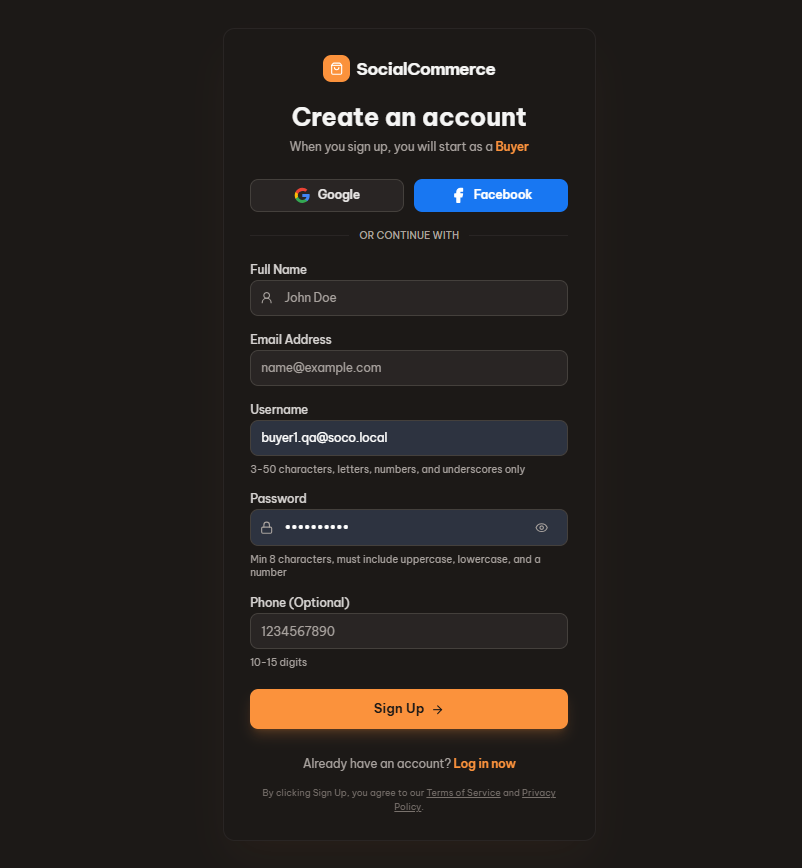
\includegraphics[width=\textwidth]{Images/UI/module1/register-page.png}
\caption{Giao diện đăng ký tài khoản}
\label{fig}
\end{figure}

\subsection{Trang Đăng nhập}

Trang đăng nhập cho phép người dùng truy cập vào hệ thống bằng tài khoản đã đăng ký trước đó. Người dùng có thể đăng nhập thông qua email hoặc tên đăng nhập kết hợp với mật khẩu tương ứng. Giao diện cũng hỗ trợ các chức năng như ghi nhớ đăng nhập và khôi phục mật khẩu trong trường hợp người dùng quên thông tin tài khoản.

Để tăng cường tính bảo mật cho hệ thống, chức năng xác thực hai lớp (2FA) qua email được hỗ trợ đối với các tài khoản đã kích hoạt tính năng này. Sau khi người dùng nhập đúng thông tin đăng nhập, hệ thống sẽ gửi mã OTP gồm 6 chữ số đến địa chỉ email đã đăng ký. Người dùng cần nhập chính xác mã OTP để hoàn tất quá trình xác thực và truy cập vào hệ thống.

Giao diện xác thực 2FA hiển thị ô nhập mã OTP, bộ đếm thời gian hiệu lực của mã và chức năng gửi lại mã xác thực khi cần thiết. Cơ chế này giúp hạn chế các truy cập trái phép và nâng cao độ an toàn cho tài khoản người dùng.

\begin{figure}[H]
\centering
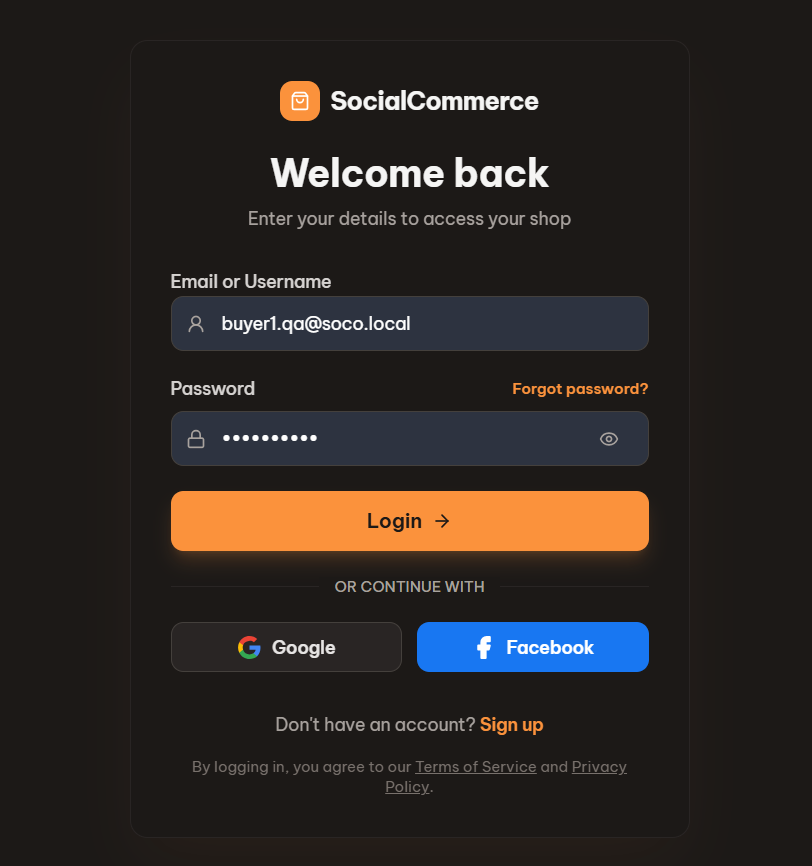
\includegraphics[width=\textwidth]{Images/UI/module1/login-page.png}
\caption{Giao diện đăng nhập của hệ thống}
\label{fig}
\end{figure}

\begin{figure}[H]
\centering
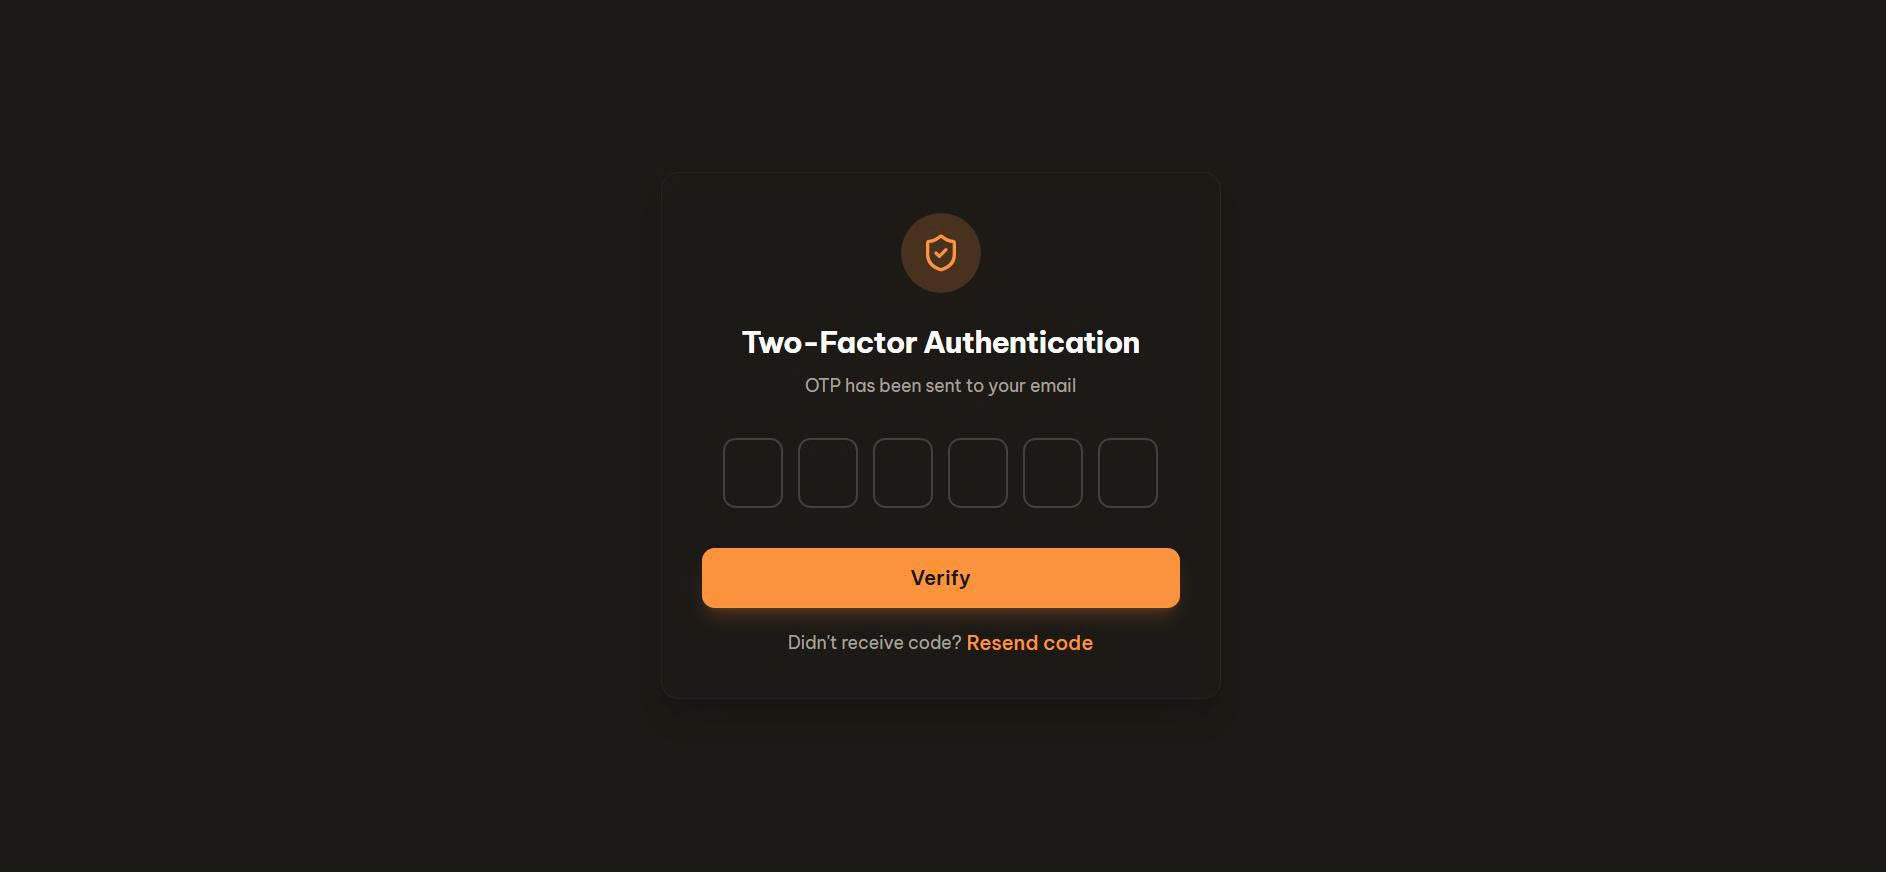
\includegraphics[width=\textwidth]{Images/UI/module1/two-factor-authentication.png}
\caption{Giao diện xác thực hai lớp (2FA)}
\label{fig}
\end{figure}

\subsection{Trang Quên mật khẩu}
Trang quên mật khẩu hỗ trợ người dùng khôi phục lại tài khoản trong trường hợp không thể đăng nhập do quên mật khẩu. Quy trình khôi phục được thực hiện thông qua email nhằm đảm bảo tính bảo mật và xác thực đúng chủ sở hữu tài khoản.

Người dùng cần nhập địa chỉ email đã đăng ký để nhận mã OTP xác thực từ hệ thống. Sau khi nhập đúng mã OTP còn hiệu lực, người dùng có thể thiết lập mật khẩu mới để tiếp tục sử dụng tài khoản. Hệ thống đồng thời kiểm tra tính hợp lệ và độ an toàn của mật khẩu mới trước khi cập nhật vào cơ sở dữ liệu.

Giao diện được xây dựng theo quy trình từng bước nhằm giúp người dùng dễ dàng thao tác và hạn chế các lỗi trong quá trình khôi phục mật khẩu.

\begin{figure}[H]
\centering
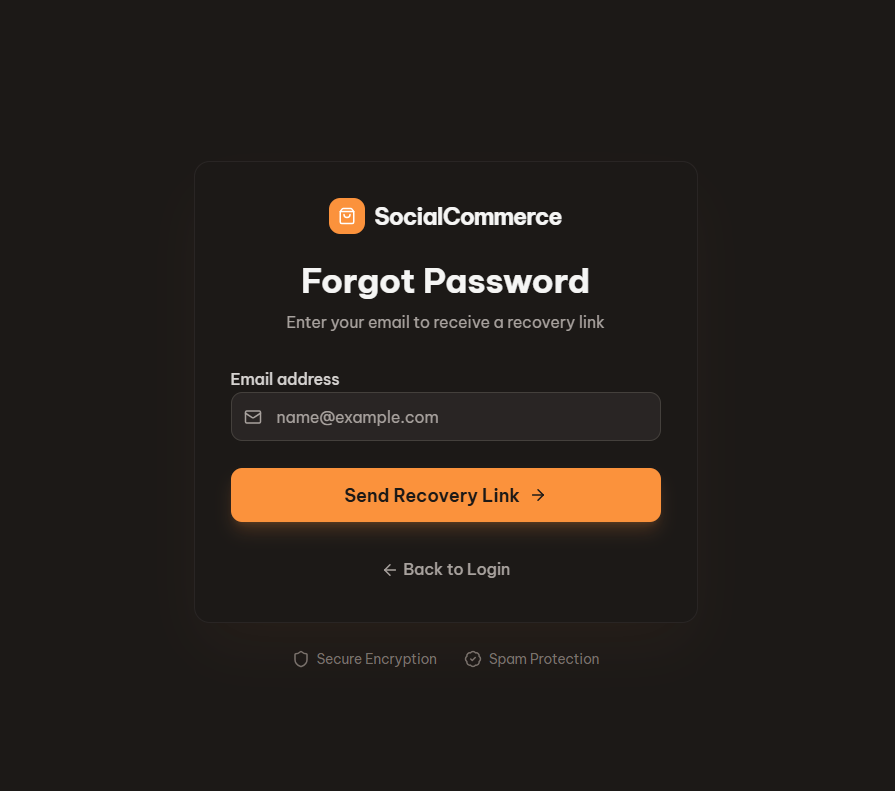
\includegraphics[width=\textwidth]{Images/UI/module1/forgot-password-page.png}
\caption{Giao diện khôi phục mật khẩu}
\label{fig}
\end{figure}

\subsection{Trang Hồ sơ cá nhân}

Trang hồ sơ cá nhân cho phép người dùng quản lý và hiển thị các thông tin liên quan đến tài khoản của mình trên hệ thống Social Commerce. Giao diện hồ sơ được phân chia thành hai loại tùy theo vai trò của người dùng bao gồm hồ sơ người mua và hồ sơ người bán.

\textbf{Hồ sơ Người mua (Buyer Profile):} Giao diện hiển thị các thông tin cơ bản của người dùng như ảnh đại diện, ảnh bìa, tên hiển thị, mô tả cá nhân, số lượng người theo dõi, số lượng đang theo dõi và danh sách các bài đăng đã chia sẻ trên hệ thống. Người dùng có thể chỉnh sửa thông tin cá nhân trực tiếp thông qua giao diện hồ sơ nhằm cá nhân hóa trải nghiệm sử dụng.

\textbf{Hồ sơ Người bán (Seller Profile):} Ngoài các thông tin cơ bản tương tự hồ sơ người mua, hồ sơ người bán còn hiển thị thêm danh sách sản phẩm đang kinh doanh, thông tin đánh giá từ khách hàng và các chỉ số liên quan đến hoạt động bán hàng. Các đánh giá và nhận xét từ người mua giúp tăng độ tin cậy cho cửa hàng và hỗ trợ người dùng khác trong quá trình tham khảo sản phẩm trước khi mua hàng.

Giao diện hồ sơ được xây dựng theo hướng trực quan và tối ưu trải nghiệm người dùng, đồng thời hỗ trợ hiển thị tốt trên nhiều loại thiết bị khác nhau.

\begin{figure}[H]
\centering
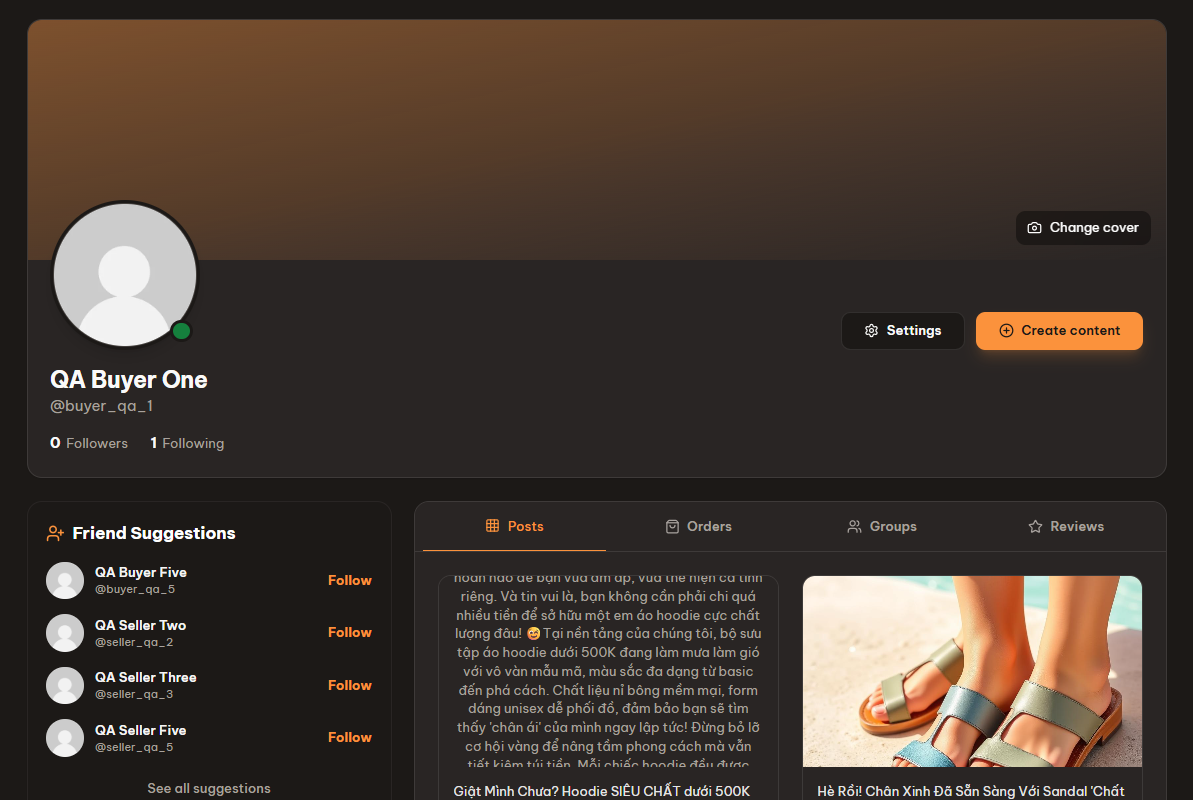
\includegraphics[width=\textwidth]{Images/UI/module1/buyer-profile.png}
\caption{Giao diện hồ sơ người mua}
\label{fig}
\end{figure}

\begin{figure}[H]
\centering
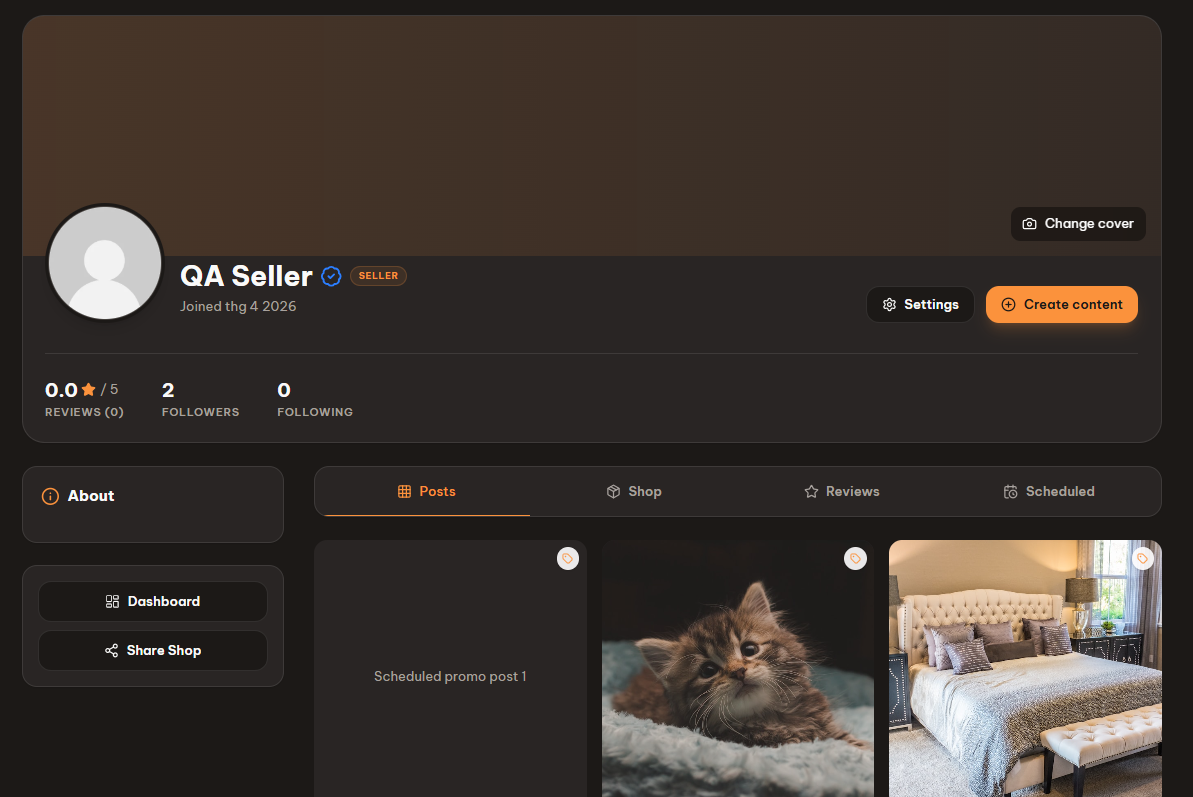
\includegraphics[width=\textwidth]{Images/UI/module1/seller-profile.png}
\caption{Giao diện hồ sơ người bán}
\label{fig}
\end{figure}

\subsection{Trang Cài đặt}

Trang cài đặt cho phép người dùng quản lý các thông tin và tùy chọn liên quan đến tài khoản cá nhân. Giao diện được tổ chức theo từng nhóm chức năng nhằm giúp người dùng dễ dàng thao tác và quản lý thông tin trên hệ thống.

Người dùng có thể cập nhật thông tin cá nhân, thay đổi mật khẩu, cấu hình quyền riêng tư và quản lý các tùy chọn thông báo. Các thay đổi sẽ được kiểm tra tính hợp lệ trước khi cập nhật vào cơ sở dữ liệu nhằm đảm bảo tính chính xác và an toàn cho dữ liệu người dùng.

\begin{figure}[H]
\centering
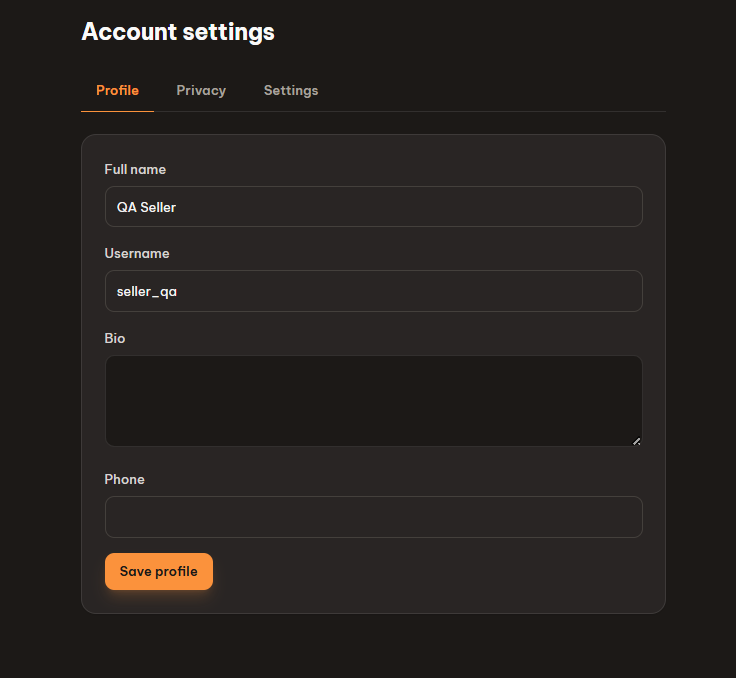
\includegraphics[width=\textwidth]{Images/UI/module1/settings-page.png}
\caption{Giao diện cài đặt tài khoản}
\label{fig}
\end{figure}

\subsection{Trang Đăng ký Người bán}

Chức năng đăng ký người bán cho phép người dùng nâng cấp tài khoản cá nhân thành tài khoản người bán để sử dụng các chức năng thương mại trên hệ thống như quản lý sản phẩm, quản lý đơn hàng và theo dõi hoạt động kinh doanh.

Quy trình đăng ký được xây dựng theo dạng nhiều bước nhằm giúp người dùng dễ dàng cung cấp đầy đủ các thông tin cần thiết và tăng tính trực quan trong quá trình đăng ký. Hệ thống bao gồm ba bước chính: thông tin cửa hàng, xác minh danh tính và thiết lập thanh toán.

Ở bước đầu tiên, người dùng cần cung cấp các thông tin cơ bản của cửa hàng như tên cửa hàng, danh mục kinh doanh, mô tả, địa chỉ liên hệ, logo và ảnh bìa đại diện cho cửa hàng. Các hình ảnh tải lên sẽ được lưu trữ thông qua dịch vụ Cloudinary nhằm hỗ trợ quản lý và hiển thị dữ liệu hiệu quả.

\begin{figure}[H]
\centering
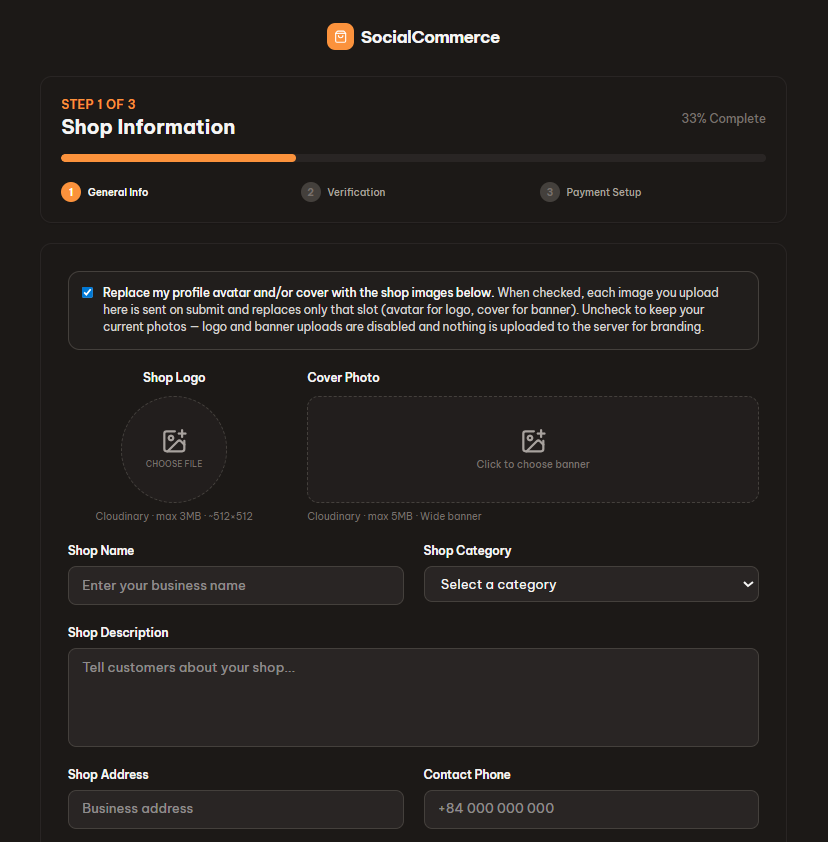
\includegraphics[width=\textwidth]{Images/UI/module1/become-seller-step1.png}
\caption{Giao diện đăng ký người bán - Bước 1: Thông tin cửa hàng}
\label{fig}
\end{figure}

Ở bước thứ hai, người dùng thực hiện xác minh danh tính bằng cách cung cấp thông tin giấy tờ xác thực như căn cước công dân, hộ chiếu hoặc giấy phép kinh doanh. Hệ thống hỗ trợ tải lên hình ảnh giấy tờ nhằm phục vụ quá trình xét duyệt và đảm bảo tính minh bạch cho tài khoản người bán.

\begin{figure}[H]
\centering
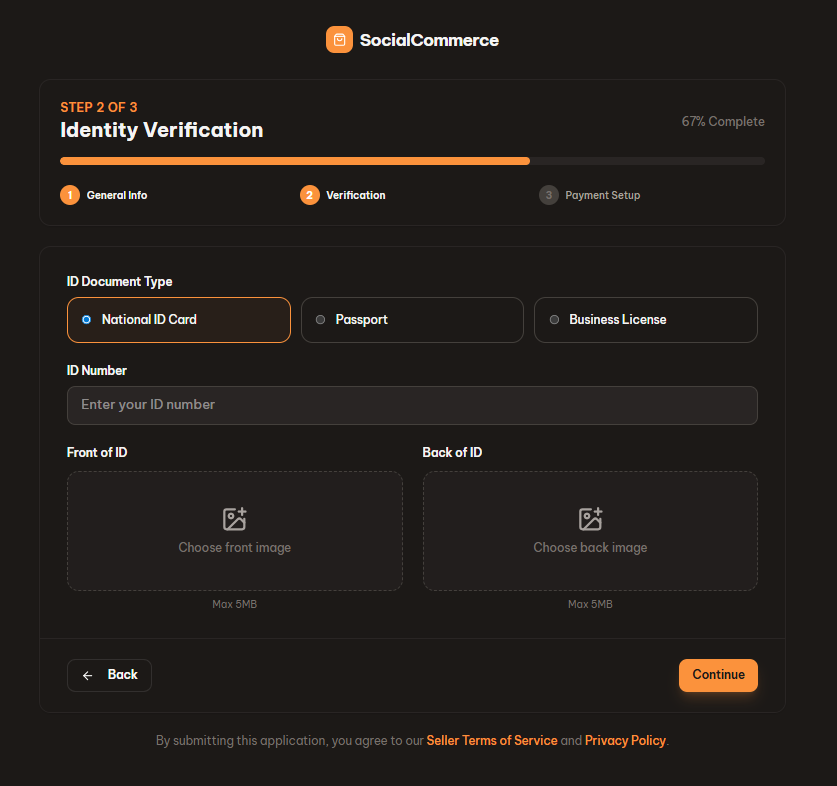
\includegraphics[width=\textwidth]{Images/UI/module1/become-seller-step2.png}
\caption{Giao diện đăng ký người bán - Bước 2: Xác minh danh tính}
\label{fig}
\end{figure}

Ở bước cuối cùng, người dùng thiết lập thông tin thanh toán bao gồm tên ngân hàng, số tài khoản và tên chủ tài khoản để phục vụ cho quá trình thanh toán và đối soát doanh thu trên hệ thống.

\begin{figure}[H]
\centering
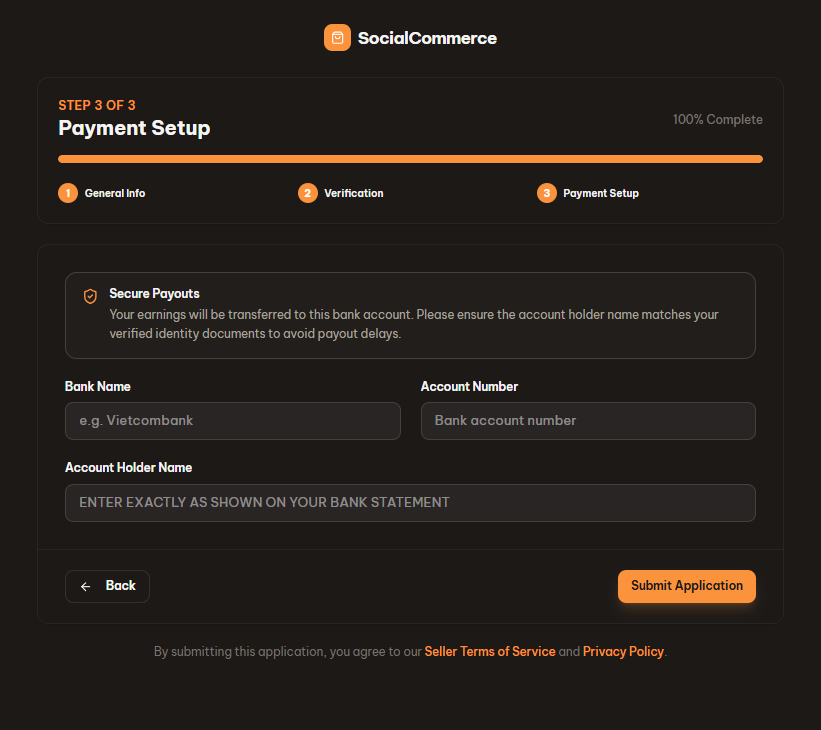
\includegraphics[width=\textwidth]{Images/UI/module1/become-seller-step3.png}
\caption{Giao diện đăng ký người bán - Bước 3: Thiết lập thanh toán}
\label{fig}
\end{figure}

Sau khi hoàn tất toàn bộ thông tin đăng ký, hệ thống sẽ gửi yêu cầu xét duyệt đến quản trị viên. Người dùng sẽ nhận được thông báo sau khi hồ sơ được gửi thành công và chờ quá trình phê duyệt từ hệ thống quản trị.

\begin{figure}[H]
\centering
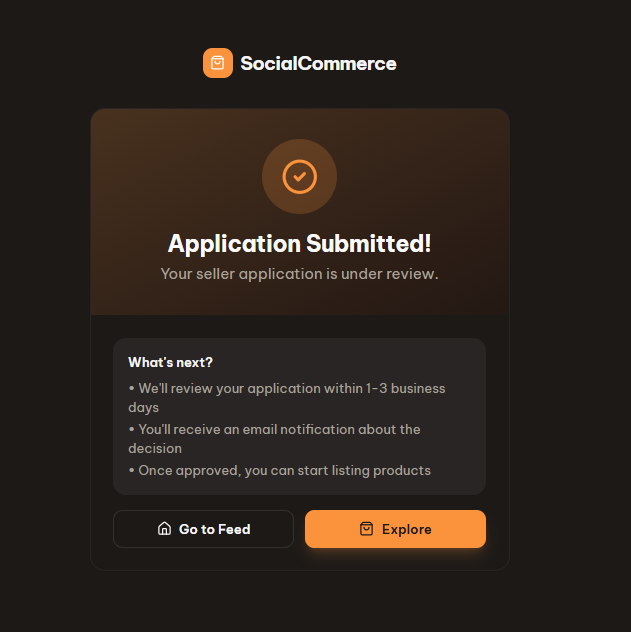
\includegraphics[width=\textwidth]{Images/UI/module1/become-seller-success.png}
\caption{Giao diện gửi đăng ký người bán thành công}
\label{fig}
\end{figure}

\section{Module 2: Tương tác Xã hội}

Module này bao gồm các chức năng hỗ trợ người dùng tương tác trên nền tảng thông qua bảng tin, tạo bài đăng, chia sẻ nội dung, bình luận và nhắn tin giữa các người dùng trong hệ thống.

\subsection{Trang chủ - Bảng tin}

Trang chủ đóng vai trò là trung tâm tương tác chính của hệ thống Social Commerce, nơi hiển thị các bài đăng mới nhất từ những người dùng và cửa hàng mà người dùng đang theo dõi. Hệ thống hỗ trợ hiển thị nội dung theo dạng bảng tin động nhằm giúp người dùng dễ dàng cập nhật các hoạt động và nội dung mới trên nền tảng.

Ngoài việc hiển thị bài đăng, giao diện còn tích hợp khu vực tạo bài viết nhanh, thanh tìm kiếm và các chức năng tương tác như thích, bình luận và chia sẻ bài đăng. Dữ liệu bảng tin được tải động và phân trang nhằm tối ưu hiệu năng hiển thị và trải nghiệm sử dụng.

\begin{figure}[H]
\centering
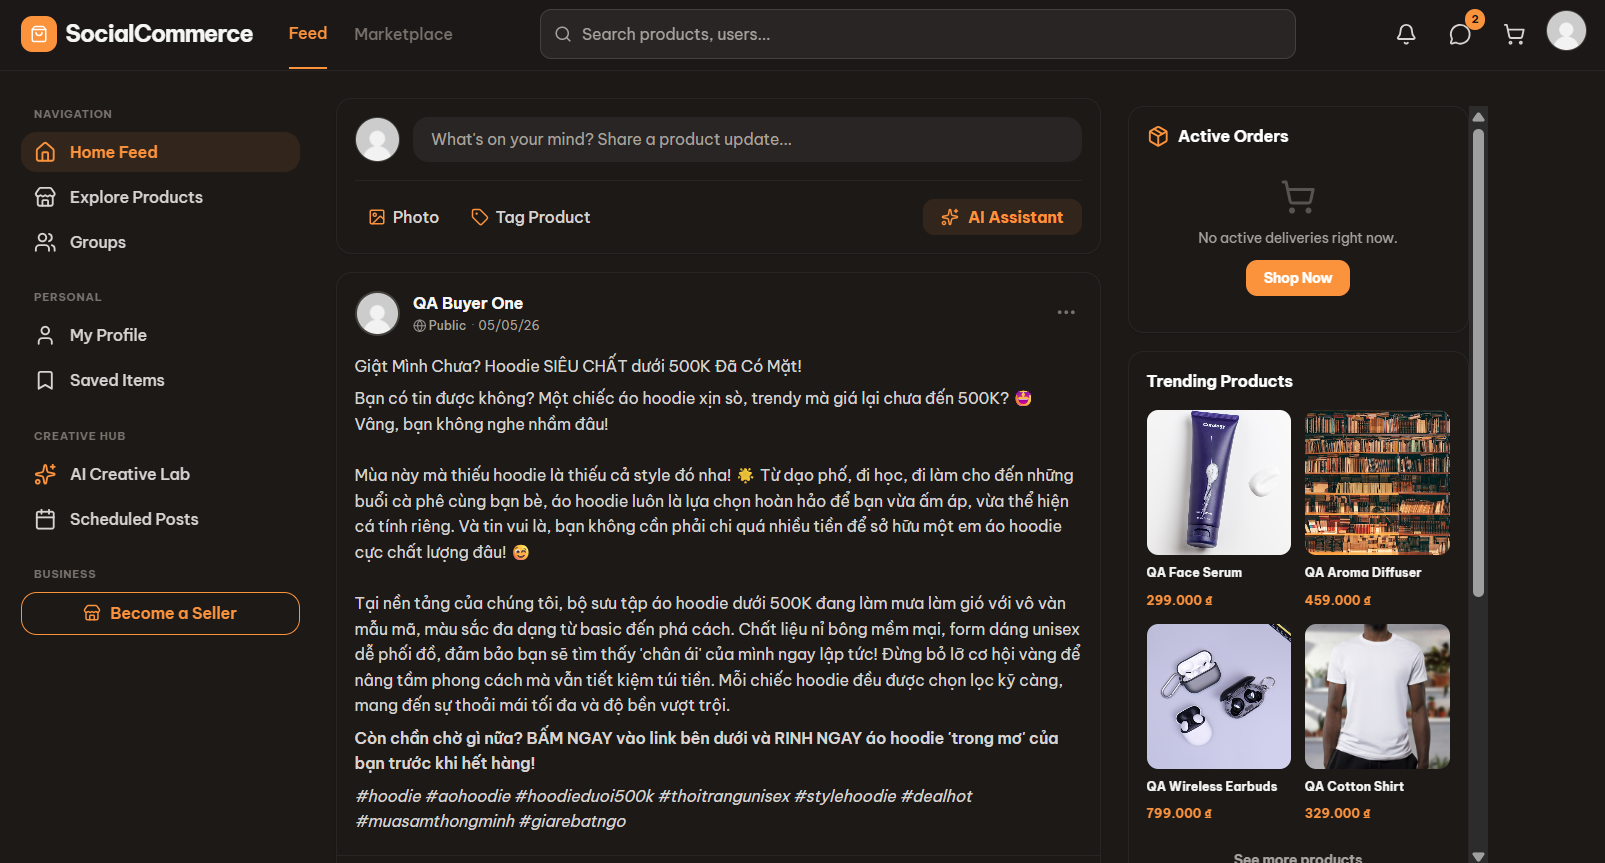
\includegraphics[width=\textwidth]{Images/UI/module2/home-feed.png}
\caption{Giao diện trang chủ - Bảng tin}
\label{fig}
\end{figure}

\subsection{Giao diện Tạo bài đăng}

Chức năng tạo bài đăng cho phép người dùng chia sẻ nội dung lên hệ thống dưới nhiều định dạng khác nhau bao gồm văn bản, hình ảnh và nội dung gắn kèm sản phẩm. Người dùng có thể nhập nội dung bài viết, tải lên hình ảnh và lựa chọn các sản phẩm liên quan để hiển thị trực tiếp trong bài đăng.

Hệ thống đồng thời hỗ trợ các tính năng mở rộng như tạo nội dung bằng AI và lên lịch đăng bài. Người dùng có thể sử dụng AI để hỗ trợ tạo nội dung văn bản, hình ảnh hoặc nội dung sáng tạo phục vụ cho hoạt động truyền thông và bán hàng trên nền tảng.

Ngoài ra, chức năng lên lịch đăng bài cho phép người dùng lựa chọn thời gian đăng tải nội dung trong tương lai. Các bài viết đã lên lịch sẽ được hệ thống tự động xử lý và đăng tải đúng thời gian đã thiết lập.

\begin{figure}[H]
\centering
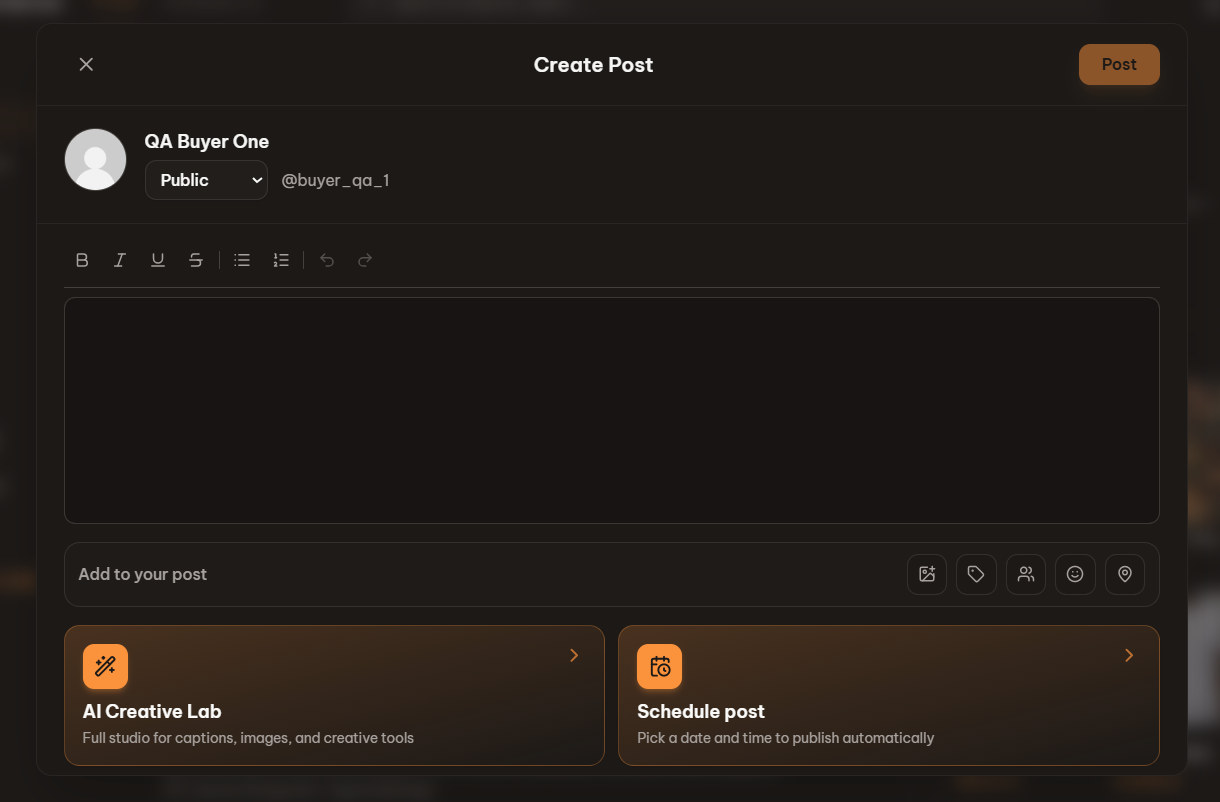
\includegraphics[width=\textwidth]{Images/UI/module2/create-post.png}
\caption{Giao diện tạo bài đăng}
\label{fig}
\end{figure}

\begin{figure}[H]
\centering
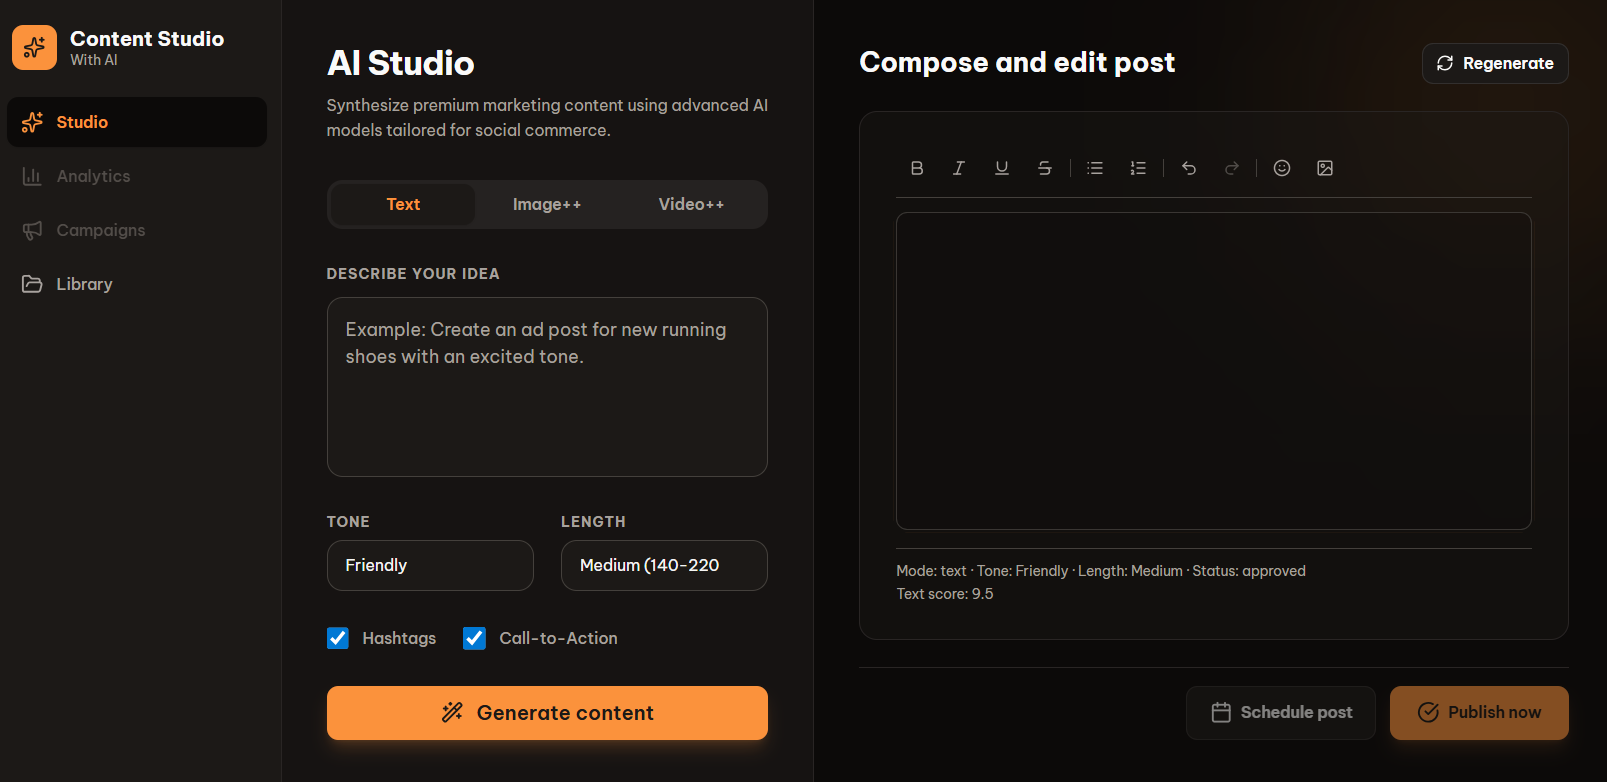
\includegraphics[width=\textwidth]{Images/UI/module2/create-post-ai-schedule.png}
\caption{Giao diện tạo bài đăng với AI và lên lịch}
\label{fig}
\end{figure}

\subsection{Trang Chi tiết Bài đăng}

Trang chi tiết bài đăng hiển thị đầy đủ nội dung của một bài viết bao gồm văn bản, hình ảnh, sản phẩm được gắn kèm và các thông tin liên quan đến người đăng bài. Người dùng có thể thực hiện các thao tác tương tác như thích bài viết, bình luận và chia sẻ nội dung trực tiếp từ giao diện này.

Hệ thống đồng thời hỗ trợ hiển thị danh sách bình luận theo thời gian thực nhằm tăng tính tương tác giữa người dùng trên nền tảng.

\begin{figure}[H]
\centering
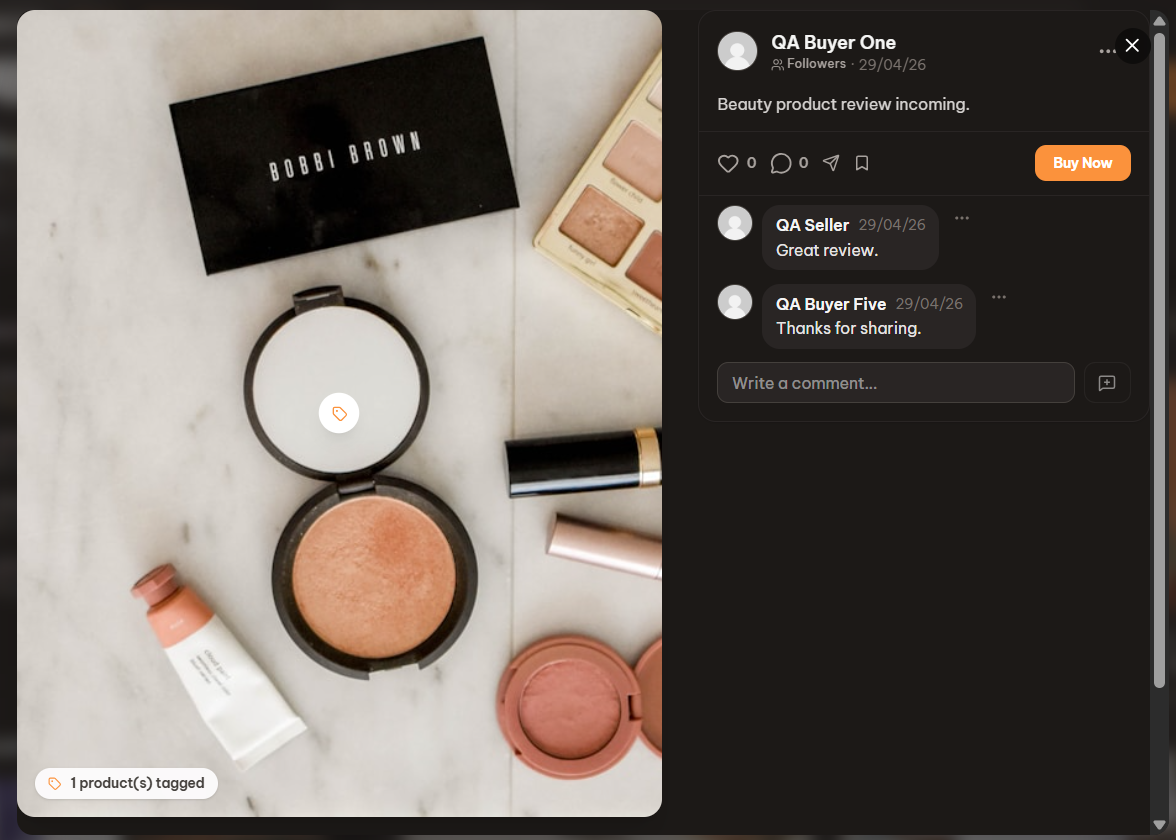
\includegraphics[width=\textwidth]{Images/UI/module2/post-detail.png}
\caption{Giao diện chi tiết bài đăng}
\label{fig}
\end{figure}

\subsection{Trang Nhắn tin}

Chức năng nhắn tin cho phép người dùng trao đổi thông tin trực tiếp với nhau ngay trên nền tảng Social Commerce. Hệ thống hỗ trợ gửi và nhận tin nhắn theo thời gian thực nhằm tăng khả năng tương tác giữa người mua và người bán trong quá trình trao đổi sản phẩm và dịch vụ.

Giao diện nhắn tin bao gồm danh sách các cuộc trò chuyện gần đây, thanh tìm kiếm và khu vực hiển thị nội dung hội thoại giữa các người dùng. Người dùng có thể theo dõi trạng thái tin nhắn chưa đọc và truy cập nhanh vào các cuộc trò chuyện trực tiếp từ giao diện hệ thống.

Hệ thống sử dụng Socket.IO để đồng bộ dữ liệu theo thời gian thực, giúp các tin nhắn mới được cập nhật trực tiếp trên giao diện mà không cần tải lại trang.

\begin{figure}[H]
\centering
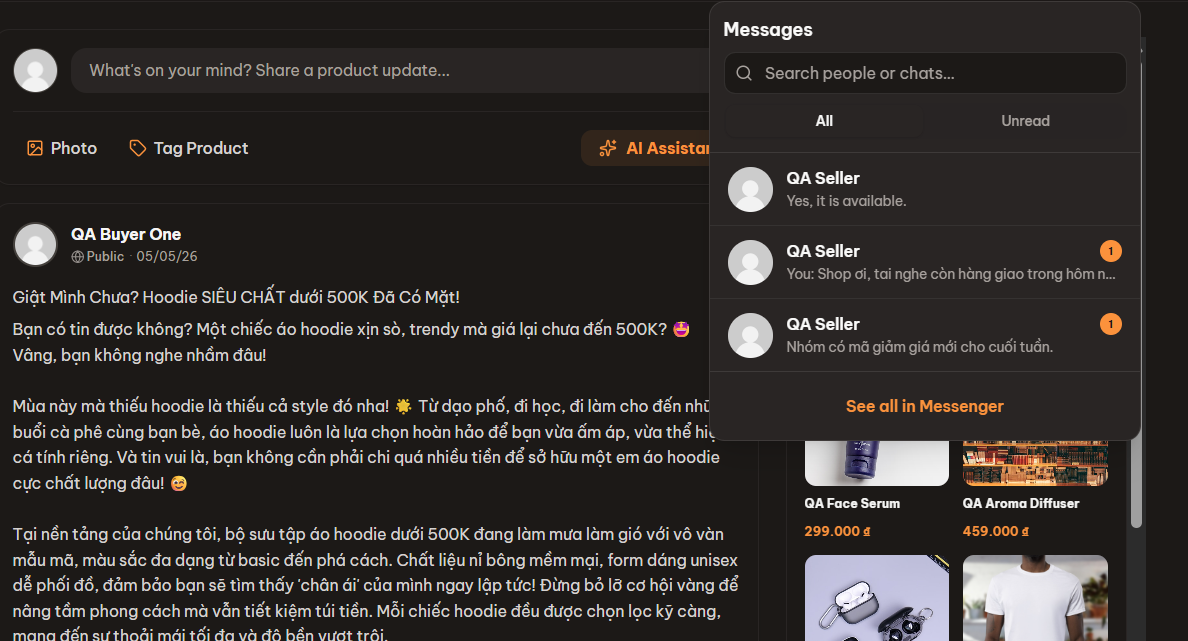
\includegraphics[width=\textwidth]{Images/UI/module2/messaging-dropdown.png}
\caption{Giao diện danh sách tin nhắn}
\label{fig}
\end{figure}

\begin{figure}[H]
\centering
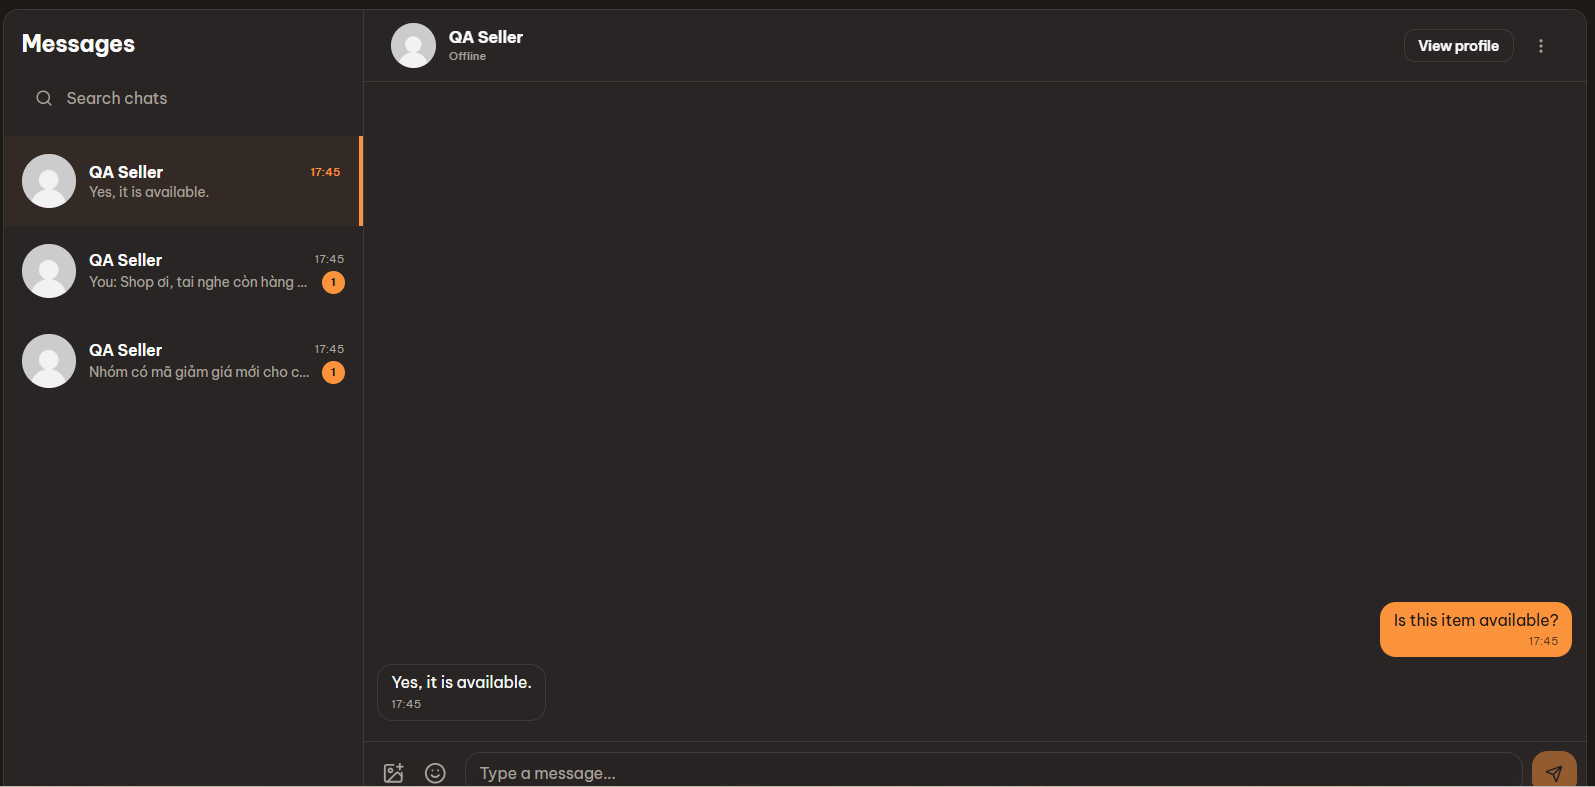
\includegraphics[width=\textwidth]{Images/UI/module2/messaging-page.png}
\caption{Giao diện trò chuyện trực tiếp}
\label{fig}
\end{figure}

\subsection{Trang Nhóm}

Chức năng nhóm cho phép người dùng tham gia vào các cộng đồng có cùng sở thích và nhu cầu trao đổi trên nền tảng Social Commerce. Hệ thống hỗ trợ tạo nhóm công khai hoặc riêng tư nhằm tăng khả năng kết nối và xây dựng cộng đồng người dùng.

Trang khám phá nhóm hiển thị danh sách các nhóm nổi bật, nhóm được đề xuất và các nhóm mà người dùng đã tham gia. Người dùng có thể tìm kiếm nhóm, xem thông tin cơ bản của từng nhóm và tham gia trực tiếp từ giao diện hệ thống.

\begin{figure}[H]
\centering
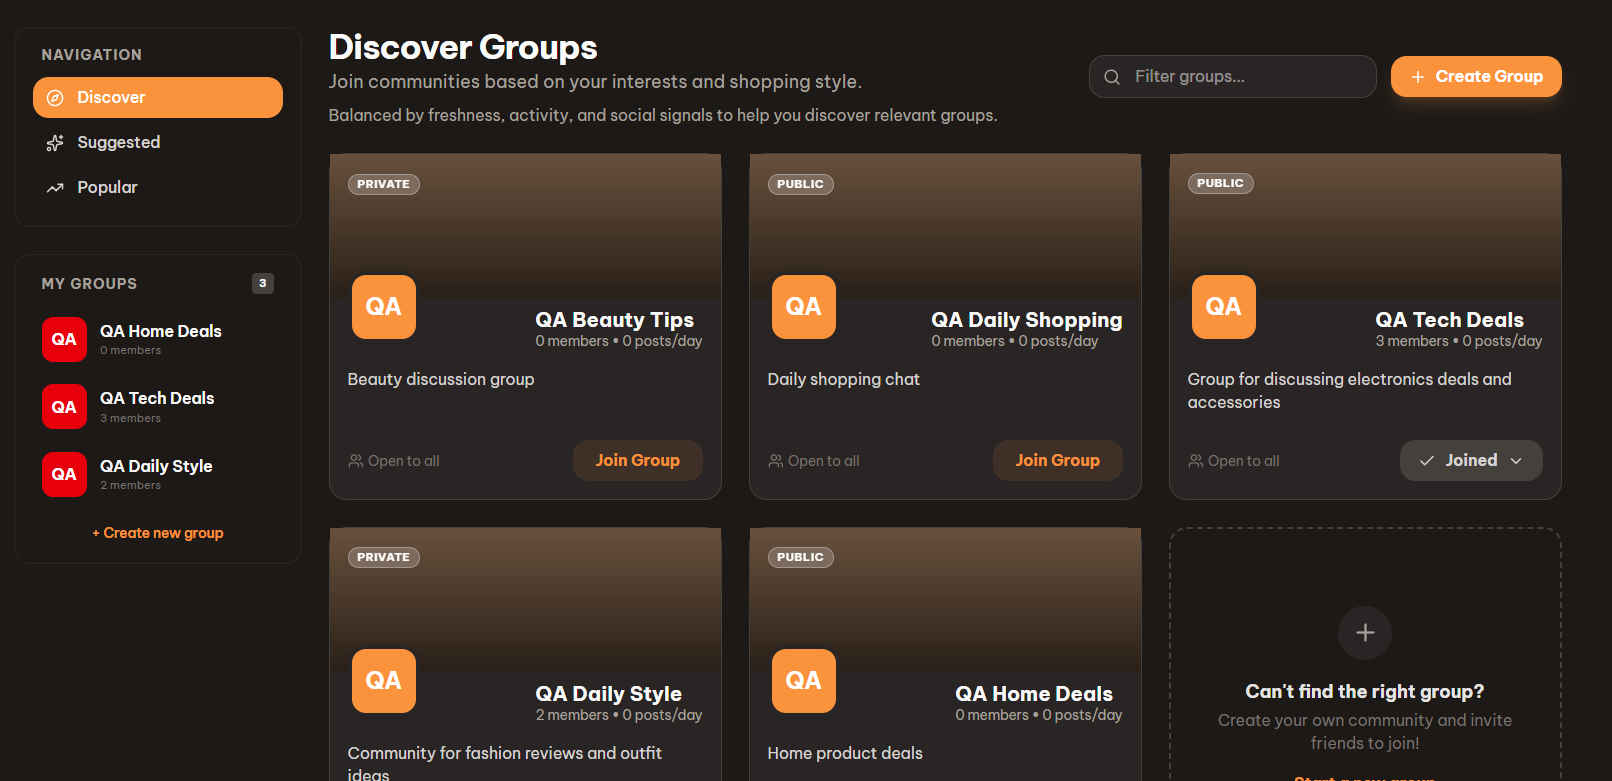
\includegraphics[width=\textwidth]{Images/UI/module2/groups-discover.png}
\caption{Giao diện khám phá nhóm}
\label{fig}
\end{figure}

Khi truy cập vào một nhóm cụ thể, hệ thống hiển thị đầy đủ các thông tin liên quan bao gồm ảnh đại diện, ảnh bìa, mô tả nhóm, danh sách thành viên và các bài đăng trong nhóm. Người dùng có thể tạo bài viết mới, chia sẻ nội dung và tương tác với các thành viên khác trong nhóm.

Ngoài ra, hệ thống còn hỗ trợ các chức năng quản lý nhóm như chỉnh sửa thông tin nhóm, thay đổi quyền riêng tư và quản lý thành viên đối với tài khoản quản trị viên nhóm.

\begin{figure}[H]
\centering
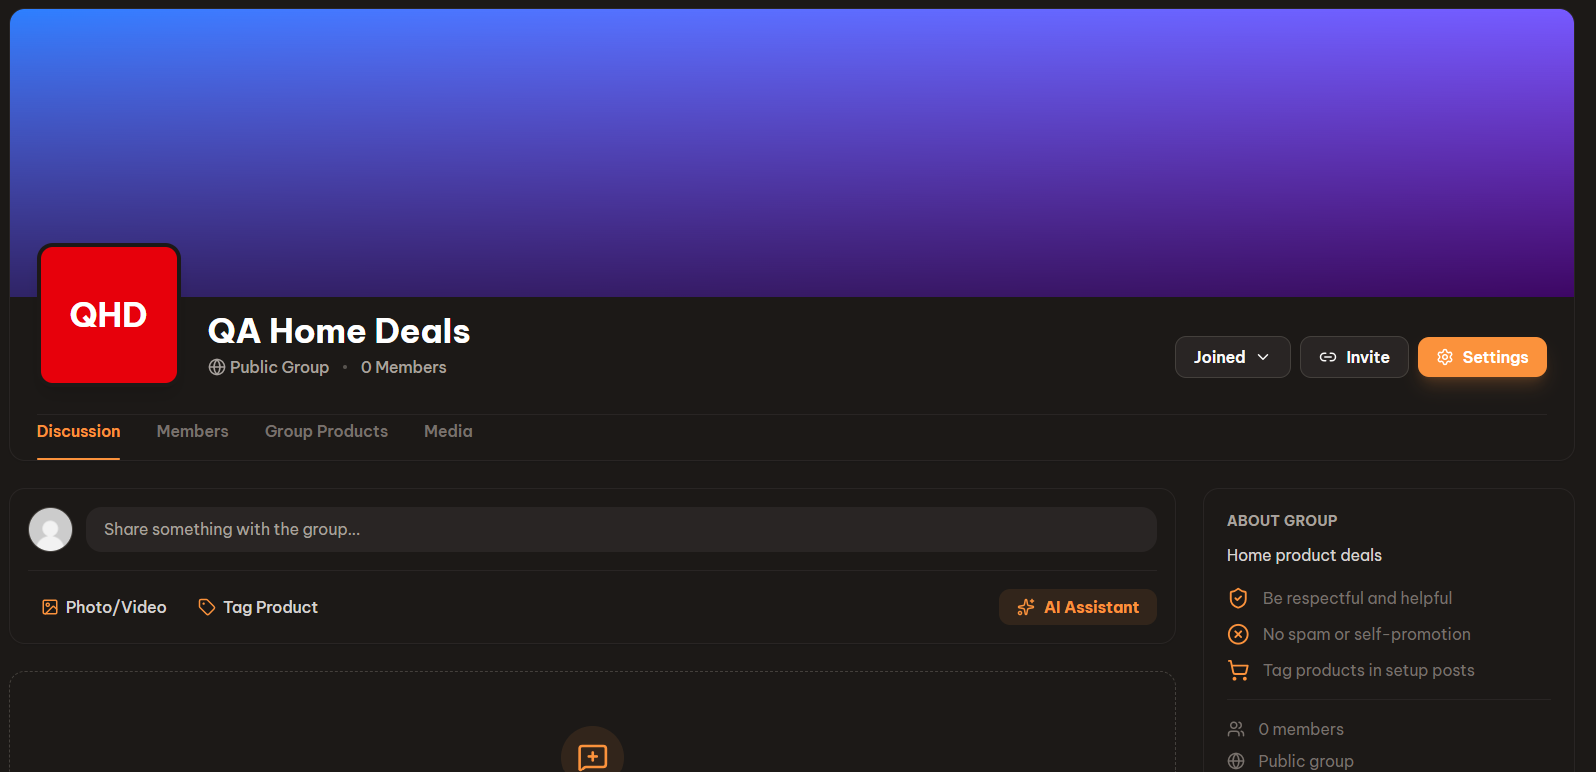
\includegraphics[width=\textwidth]{Images/UI/module2/group-detail.png}
\caption{Giao diện chi tiết nhóm}
\label{fig}
\end{figure}

\begin{figure}[H]
\centering
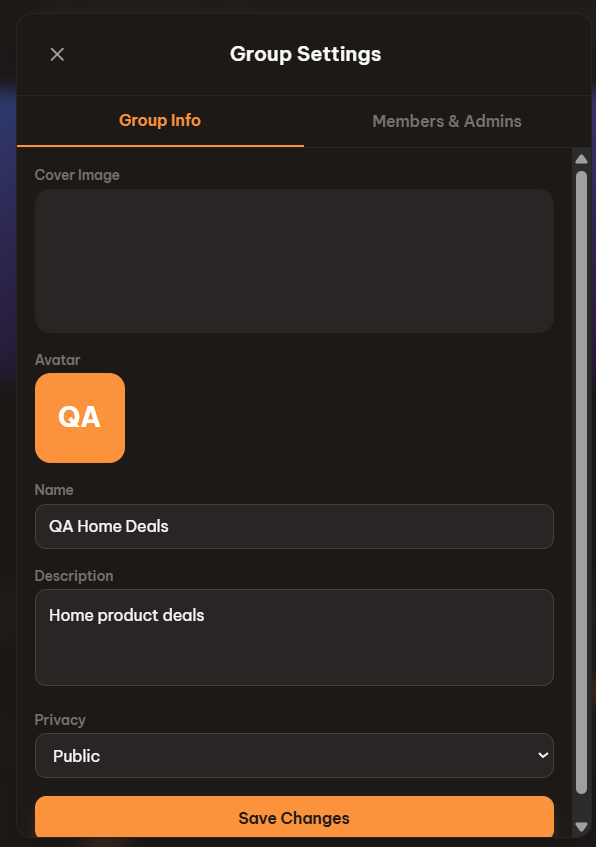
\includegraphics[width=\textwidth]{Images/UI/module2/group-settings.png}
\caption{Giao diện quản lý thông tin nhóm}
\label{fig}
\end{figure}

\subsection{Trang Tìm kiếm}

Chức năng tìm kiếm cho phép người dùng tra cứu các nội dung trên nền tảng Social Commerce bao gồm sản phẩm, bài đăng và người dùng. Hệ thống hỗ trợ tìm kiếm theo từ khóa kết hợp với cơ chế phân loại kết quả nhằm giúp người dùng dễ dàng tiếp cận nội dung phù hợp.

Giao diện tìm kiếm được tổ chức theo từng danh mục kết quả như tất cả kết quả, sản phẩm, bài đăng và người dùng. Người dùng có thể chuyển đổi nhanh giữa các danh mục để xem nội dung liên quan đến từ khóa tìm kiếm.

Đối với tìm kiếm sản phẩm, hệ thống hỗ trợ thêm các bộ lọc và sắp xếp kết quả như khoảng giá, đánh giá sản phẩm và độ liên quan của kết quả tìm kiếm. Người dùng cũng có thể sắp xếp sản phẩm theo mức độ phổ biến, mới nhất hoặc giá bán nhằm tối ưu trải nghiệm mua sắm trên nền tảng.

\begin{figure}[H]
\centering
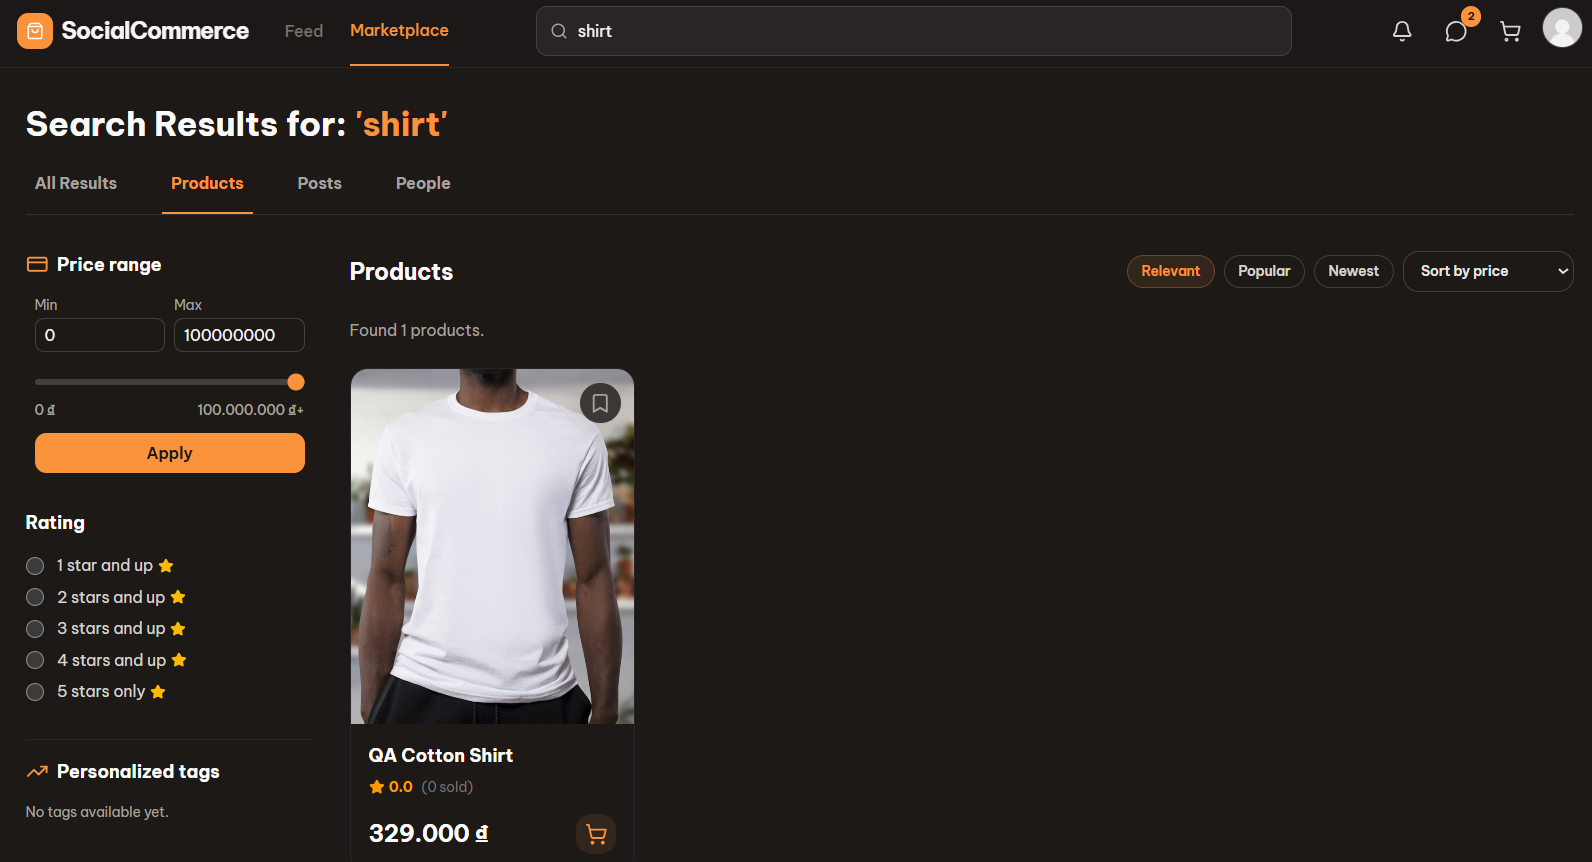
\includegraphics[width=\textwidth]{Images/UI/module2/search-page.png}
\caption{Giao diện tìm kiếm trên hệ thống}
\label{fig}
\end{figure}

\section{Module 3: Hoạt động Thương mại}

Module hoạt động thương mại là thành phần cốt lõi của hệ thống Social Commerce, hỗ trợ các chức năng liên quan đến mua bán sản phẩm, quản lý cửa hàng, xử lý đơn hàng và theo dõi hoạt động kinh doanh trên nền tảng.

Hệ thống cho phép người dùng khám phá sản phẩm, tìm kiếm và lọc sản phẩm theo nhiều tiêu chí khác nhau, thêm sản phẩm vào giỏ hàng, thực hiện thanh toán và theo dõi trạng thái đơn hàng. Đối với người bán, hệ thống cung cấp các công cụ quản lý cửa hàng, quản lý sản phẩm, theo dõi doanh thu và xử lý đơn hàng trực tiếp trên nền tảng.

\subsection{Trang Khám phá Sản phẩm}

Trang khám phá sản phẩm hiển thị danh sách các sản phẩm đang được kinh doanh trên nền tảng dưới dạng lưới trực quan. Mỗi sản phẩm bao gồm hình ảnh, tên sản phẩm, giá bán, đánh giá và các thông tin liên quan nhằm hỗ trợ người dùng dễ dàng tham khảo và lựa chọn sản phẩm phù hợp.

Hệ thống hỗ trợ tìm kiếm và lọc sản phẩm theo nhiều tiêu chí như khoảng giá, đánh giá, mức độ phổ biến và thời gian đăng tải. Ngoài ra, người dùng có thể lưu sản phẩm yêu thích, xem nhanh thông tin sản phẩm và truy cập trực tiếp đến trang chi tiết sản phẩm từ giao diện khám phá.

Dữ liệu sản phẩm được tải động kết hợp với cơ chế phân trang và sắp xếp nhằm tối ưu hiệu năng hiển thị và trải nghiệm mua sắm trên nền tảng.

\begin{figure}[H]
\centering
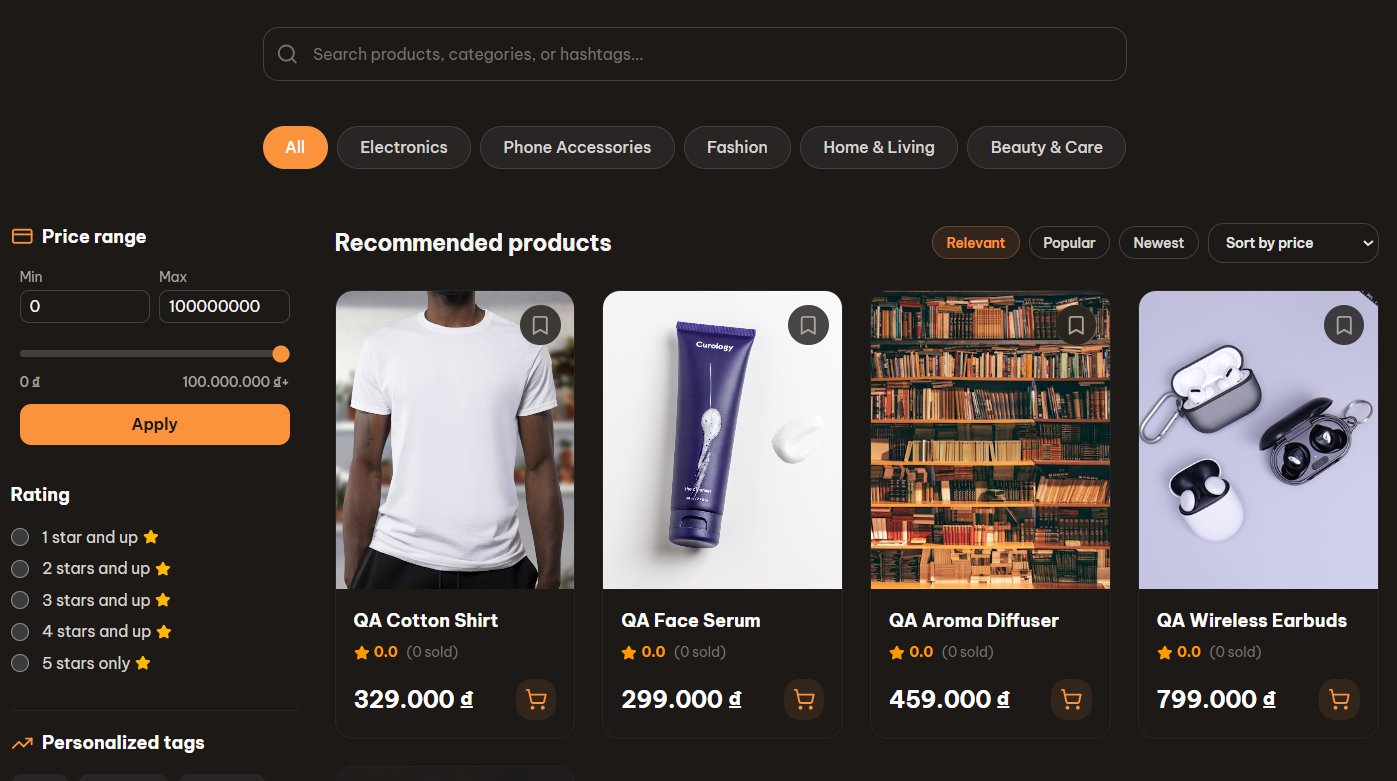
\includegraphics[width=\textwidth]{Images/UI/module3/product-explore.png}
\caption{Giao diện khám phá sản phẩm}
\label{fig:module3-product-explore}
\end{figure}

\subsection{Trang Chi tiết Sản phẩm}

Trang chi tiết sản phẩm cung cấp đầy đủ thông tin liên quan đến một sản phẩm cụ thể bao gồm hình ảnh, mô tả, giá bán, thông tin cửa hàng và đánh giá từ người mua. Người dùng có thể xem nhiều hình ảnh sản phẩm, lựa chọn biến thể sản phẩm và thực hiện các thao tác mua hàng trực tiếp từ giao diện này.

Hệ thống đồng thời hỗ trợ hiển thị đánh giá sản phẩm, số lượng đã bán, thông tin người bán và các sản phẩm liên quan nhằm tăng trải nghiệm mua sắm và hỗ trợ người dùng trong quá trình tham khảo sản phẩm.

Ngoài ra, người dùng có thể thêm sản phẩm vào giỏ hàng, lưu sản phẩm yêu thích hoặc chia sẻ sản phẩm trực tiếp thông qua giao diện chi tiết sản phẩm.

\begin{figure}[H]
\centering
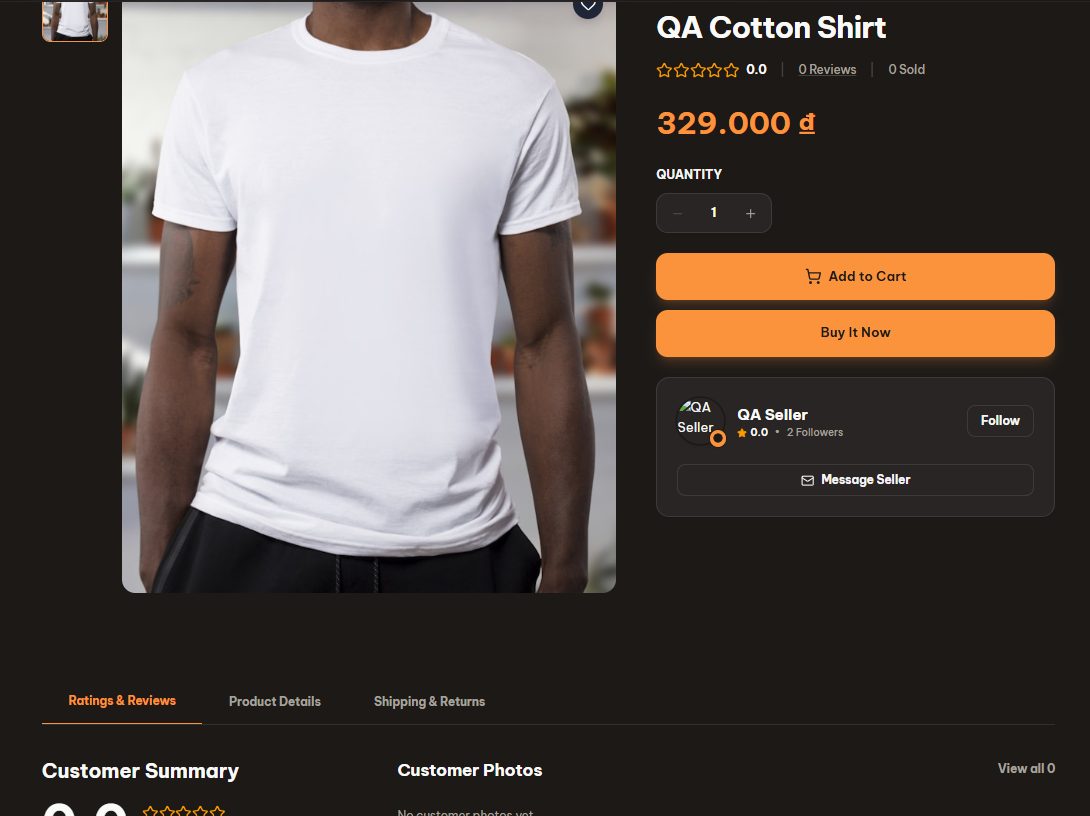
\includegraphics[width=\textwidth]{Images/UI/module3/product-detail.png}
\caption{Giao diện chi tiết sản phẩm}
\label{fig:module3-product-detail}
\end{figure}

\subsubsection{Trang Giỏ hàng}

Trang giỏ hàng cho phép người dùng quản lý các sản phẩm đã lựa chọn trước khi thực hiện thanh toán. Hệ thống hiển thị đầy đủ thông tin của từng sản phẩm bao gồm hình ảnh, tên sản phẩm, giá bán, số lượng và tổng giá trị đơn hàng.

Người dùng có thể thay đổi số lượng sản phẩm, xóa sản phẩm khỏi giỏ hàng hoặc tiếp tục mua sắm trực tiếp từ giao diện này. Hệ thống đồng thời tự động cập nhật tổng tiền dựa trên các thay đổi trong giỏ hàng nhằm hỗ trợ người dùng dễ dàng theo dõi chi phí đơn hàng.

Ngoài ra, giỏ hàng còn hỗ trợ lưu trạng thái sản phẩm theo tài khoản người dùng nhằm đảm bảo dữ liệu được đồng bộ giữa các phiên đăng nhập khác nhau trên hệ thống.

\begin{figure}[H]
\centering
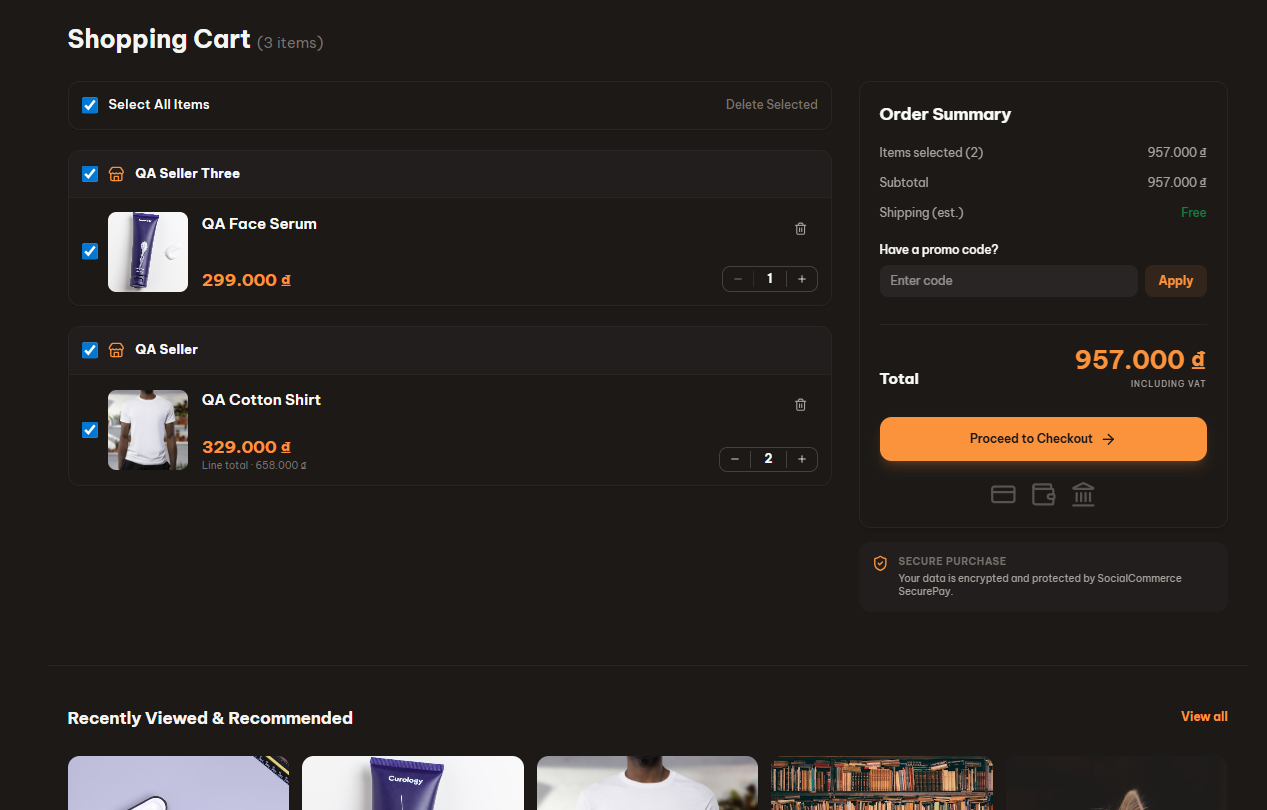
\includegraphics[width=\textwidth]{Images/UI/module3/cart-page.png}
\caption{Giao diện giỏ hàng}
\label{fig:module3-cart-page}
\end{figure}

\subsubsection{Trang Thanh toán}

Trang thanh toán hỗ trợ người dùng hoàn tất quá trình đặt hàng thông qua quy trình xác nhận đơn hàng trực quan và thuận tiện. Hệ thống hiển thị thông tin sản phẩm, địa chỉ giao hàng, phương thức thanh toán và tổng giá trị đơn hàng trước khi xác nhận thanh toán.

Người dùng có thể lựa chọn hoặc cập nhật địa chỉ nhận hàng, kiểm tra thông tin sản phẩm và xác nhận đơn hàng trực tiếp trên giao diện thanh toán. Sau khi thanh toán thành công, hệ thống sẽ tạo đơn hàng và cập nhật trạng thái đơn hàng tương ứng trong cơ sở dữ liệu.

Quy trình thanh toán được xây dựng theo từng bước nhằm giúp người dùng dễ dàng theo dõi thông tin và hạn chế sai sót trong quá trình đặt hàng.

\begin{figure}[H]
\centering
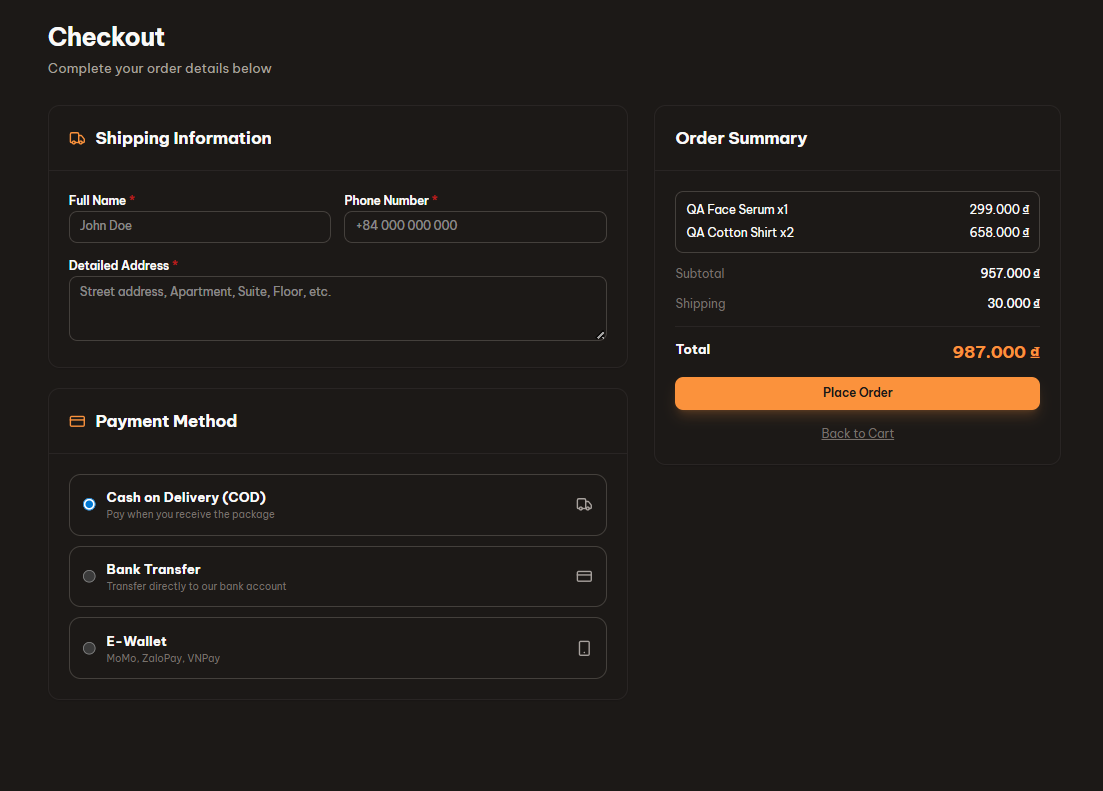
\includegraphics[width=\textwidth]{Images/UI/module3/checkout-page.png}
\caption{Giao diện thanh toán đơn hàng}
\label{fig:module3-checkout-page}
\end{figure}

\subsubsection{Trang Quản lý Cửa hàng}

Trang quản lý cửa hàng cung cấp giao diện tổng quan dành cho người bán nhằm theo dõi hoạt động kinh doanh trên nền tảng. Hệ thống hỗ trợ quản lý sản phẩm, quản lý đơn hàng và theo dõi các thống kê liên quan đến hoạt động bán hàng.

Người bán có thể xem nhanh số lượng đơn hàng, doanh thu, trạng thái sản phẩm và các thông tin thống kê trực tiếp từ giao diện quản lý. Ngoài ra, hệ thống còn hỗ trợ điều hướng nhanh đến các chức năng quản lý sản phẩm và xử lý đơn hàng nhằm tối ưu quá trình vận hành cửa hàng.

Giao diện dashboard được xây dựng theo hướng trực quan, hỗ trợ hiển thị dữ liệu thống kê và hoạt động kinh doanh theo thời gian thực.

\begin{figure}[H]
\centering
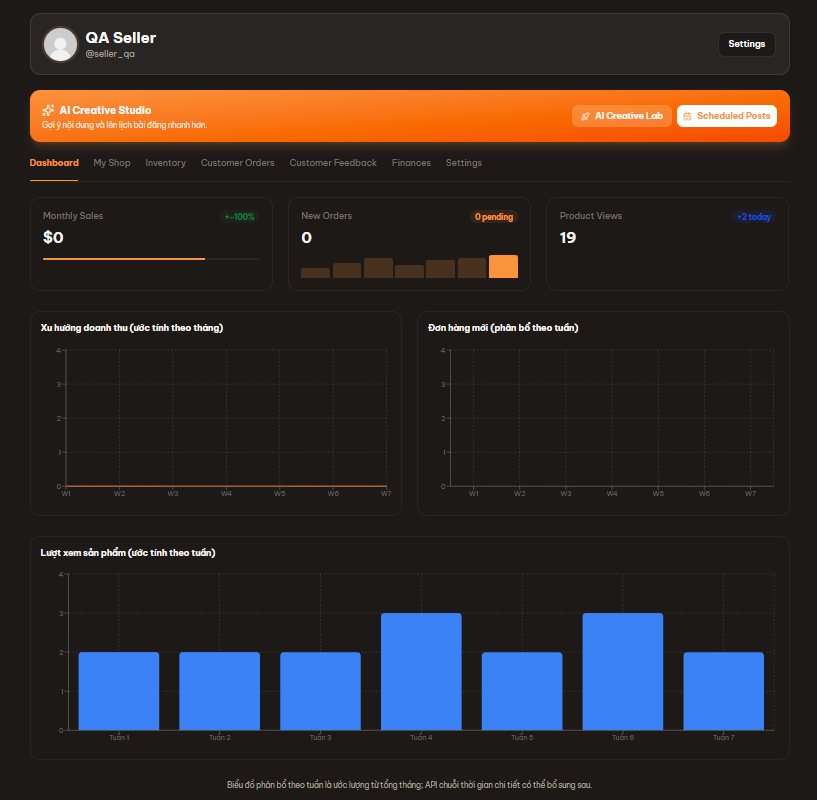
\includegraphics[width=\textwidth]{Images/UI/module3/seller-dashboard.png}
\caption{Giao diện quản lý cửa hàng}
\label{fig:module3-seller-dashboard}
\end{figure}

\subsubsection{Trang Cửa hàng của tôi}

Trang “Cửa hàng của tôi” cho phép người bán quản lý toàn bộ danh sách sản phẩm đang kinh doanh trên nền tảng Social Commerce. Giao diện hiển thị thông tin tổng quan của cửa hàng cùng danh sách sản phẩm, trạng thái hoạt động và các chỉ số liên quan đến quá trình kinh doanh.

Người bán có thể tìm kiếm sản phẩm theo tên, lọc sản phẩm theo trạng thái như đang hoạt động, bản nháp, hết hàng hoặc đã lưu trữ. Ngoài ra, hệ thống còn hỗ trợ sắp xếp danh sách sản phẩm và hiển thị các thông tin thống kê như lượt xem, số lượng đã bán và trạng thái hiện tại của từng sản phẩm.

Từ giao diện này, người bán có thể nhanh chóng thực hiện các thao tác quản lý như thêm sản phẩm mới, chỉnh sửa thông tin sản phẩm, lưu trữ sản phẩm hoặc xóa sản phẩm khỏi hệ thống.

\begin{figure}[H]
\centering
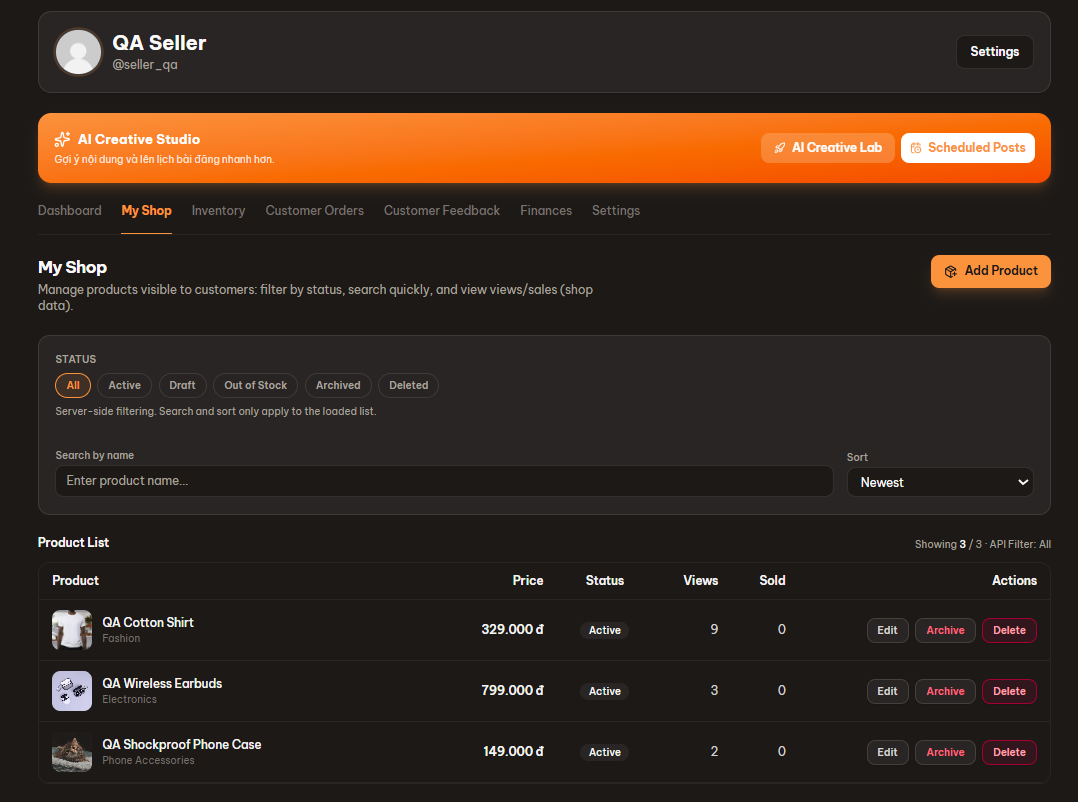
\includegraphics[width=\textwidth]{Images/UI/module3/my-shop.png}
\caption{Giao diện quản lý sản phẩm trong cửa hàng}
\label{fig}
\end{figure}

\subsubsection{Trang Tạo và Chỉnh sửa Sản phẩm}

Chức năng tạo và chỉnh sửa sản phẩm cho phép người bán quản lý thông tin sản phẩm trực tiếp trên nền tảng Social Commerce. Người bán có thể tạo mới sản phẩm hoặc cập nhật các thông tin liên quan như tên sản phẩm, mô tả, giá bán, danh mục, hình ảnh và trạng thái hiển thị của sản phẩm.

Hệ thống hỗ trợ tải lên nhiều hình ảnh sản phẩm nhằm tăng khả năng hiển thị và hỗ trợ người mua dễ dàng tham khảo thông tin trước khi đưa ra quyết định mua hàng. Các hình ảnh sản phẩm được lưu trữ thông qua Cloudinary để tối ưu khả năng quản lý và hiển thị dữ liệu đa phương tiện.

Ngoài ra, hệ thống còn hỗ trợ cập nhật nhanh thông tin sản phẩm và đồng bộ dữ liệu trực tiếp trên giao diện quản lý cửa hàng của người bán.

\begin{figure}[H]
\centering
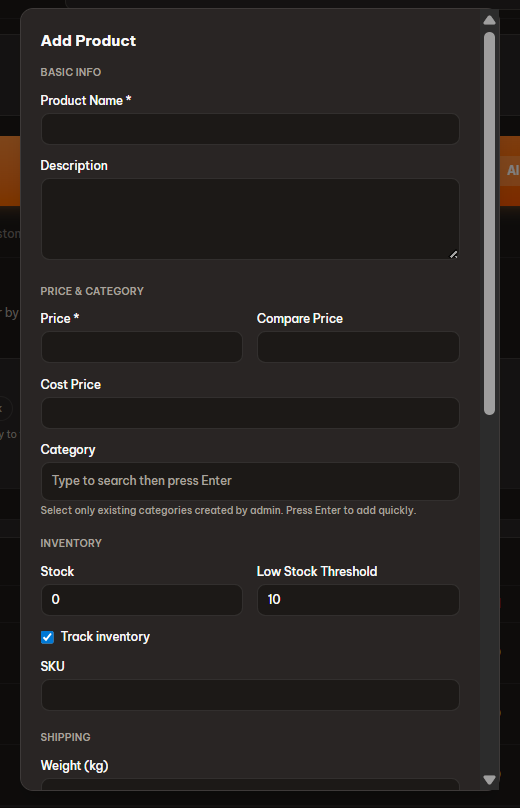
\includegraphics[width=\textwidth]{Images/UI/module3/create-product.png}
\caption{Giao diện tạo và chỉnh sửa sản phẩm}
\label{fig:module3-create-product}
\end{figure}

\subsubsection{Trang Quản lý Đơn hàng}

Trang quản lý đơn hàng cho phép người bán theo dõi và xử lý các đơn hàng phát sinh trên hệ thống. Giao diện hiển thị danh sách đơn hàng cùng với các thông tin quan trọng như mã đơn hàng, người mua, trạng thái đơn hàng, thời gian đặt hàng và tổng giá trị thanh toán.

Hệ thống hỗ trợ quản lý nhiều trạng thái đơn hàng khác nhau bao gồm chờ xác nhận, đang xử lý, đang giao hàng, đã hoàn thành và đã hủy. Người bán có thể cập nhật trạng thái đơn hàng trực tiếp từ giao diện quản lý nhằm đồng bộ tiến trình xử lý với người mua.

Ngoài ra, hệ thống còn hỗ trợ tìm kiếm và lọc đơn hàng nhằm giúp người bán dễ dàng quản lý số lượng lớn đơn hàng trên nền tảng.

\begin{figure}[H]
\centering
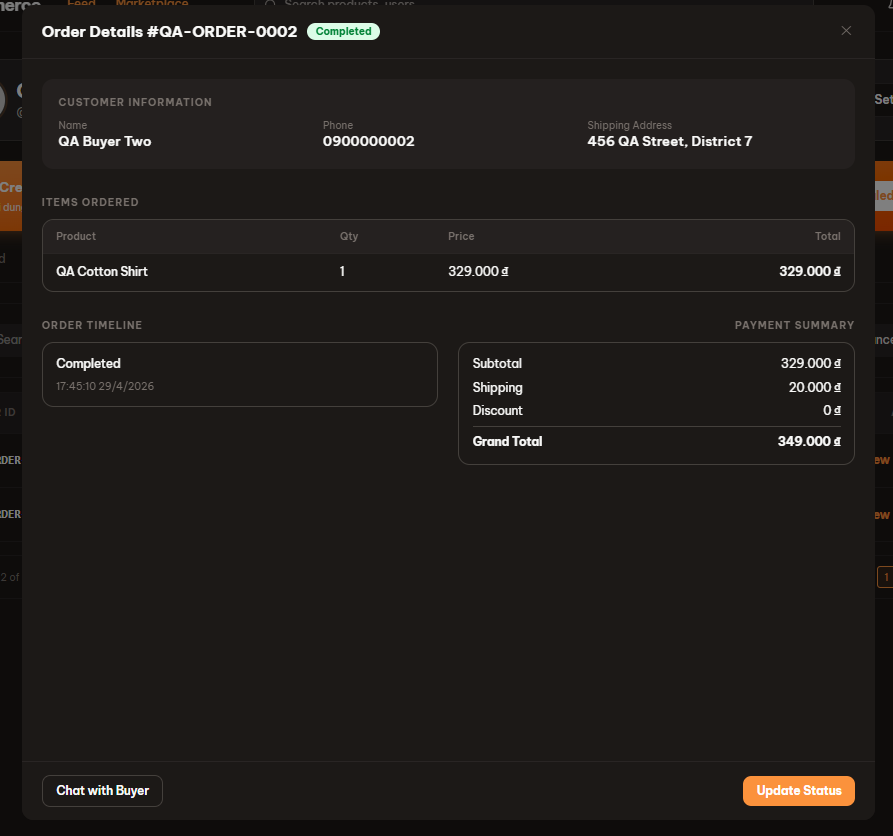
\includegraphics[width=\textwidth]{Images/UI/module3/orders-management.png}
\caption{Giao diện quản lý đơn hàng}
\label{fig:module3-orders-management}
\end{figure}


\section{Module 4: Hệ thống Quản trị}

Module quản trị được xây dựng như một hệ thống riêng biệt nhằm hỗ trợ quản trị viên theo dõi và quản lý toàn bộ hoạt động của nền tảng Social Commerce. Hệ thống quản trị sử dụng backend và frontend độc lập với hệ thống người dùng thông thường, đồng thời kết nối chung cơ sở dữ liệu để thực hiện các chức năng kiểm duyệt và vận hành hệ thống.

\subsubsection{Trang Đăng nhập Quản trị}

Trang đăng nhập quản trị cho phép quản trị viên truy cập vào hệ thống admin thông qua tài khoản quản trị riêng. Sau khi xác thực thành công, quản trị viên có thể sử dụng các chức năng quản lý người dùng, nội dung, danh mục sản phẩm và xử lý báo cáo trên hệ thống.

\begin{figure}[H]
\centering
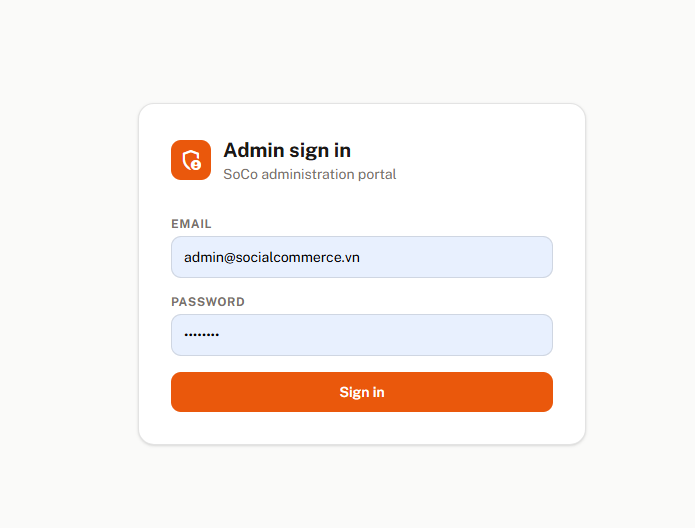
\includegraphics[width=\textwidth]{Images/UI/module4/admin-login.png}
\caption{Giao diện đăng nhập quản trị}
\label{fig:module4-admin-login}
\end{figure}

\subsubsection{Trang Dashboard Quản trị}

Trang dashboard quản trị hiển thị tổng quan các thông tin và thống kê quan trọng của hệ thống bao gồm số lượng người dùng, sản phẩm, đơn hàng và các hoạt động phát sinh trên nền tảng.

Hệ thống hỗ trợ hiển thị dữ liệu thống kê trực quan nhằm giúp quản trị viên dễ dàng theo dõi tình trạng hoạt động của hệ thống và phát hiện các vấn đề cần xử lý. Ngoài ra, dashboard còn hỗ trợ điều hướng nhanh đến các chức năng quản lý chính của hệ thống quản trị.

\begin{figure}[H]
\centering
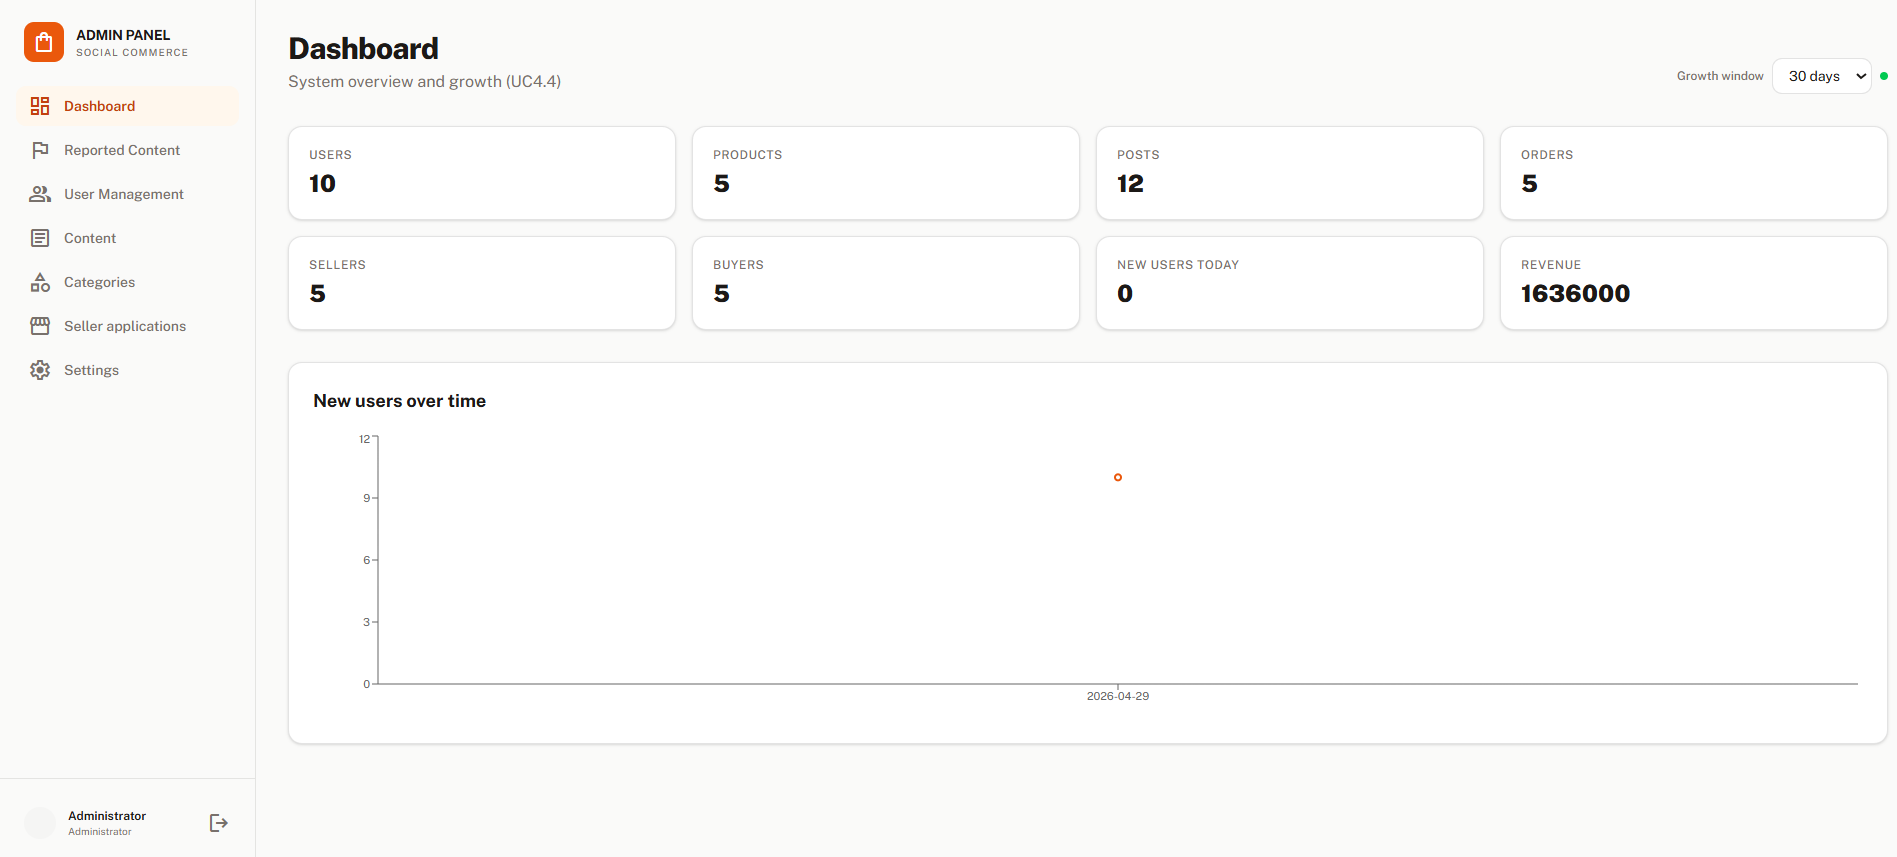
\includegraphics[width=\textwidth]{Images/UI/module4/admin-dashboard.png}
\caption{Giao diện dashboard quản trị}
\label{fig:module4-admin-dashboard}
\end{figure}

\subsubsection{Trang Quản lý Người dùng}

Trang quản lý người dùng cho phép quản trị viên theo dõi danh sách tài khoản đang hoạt động trên hệ thống. Giao diện hỗ trợ tìm kiếm, lọc và quản lý thông tin người dùng nhằm hỗ trợ quá trình vận hành nền tảng.

Quản trị viên có thể thực hiện các thao tác như xem thông tin tài khoản, khóa hoặc mở khóa tài khoản và theo dõi trạng thái hoạt động của người dùng trên hệ thống. Ngoài ra, hệ thống cũng hỗ trợ quản lý các tài khoản người bán và quá trình xét duyệt đăng ký người bán.

\begin{figure}[H]
\centering
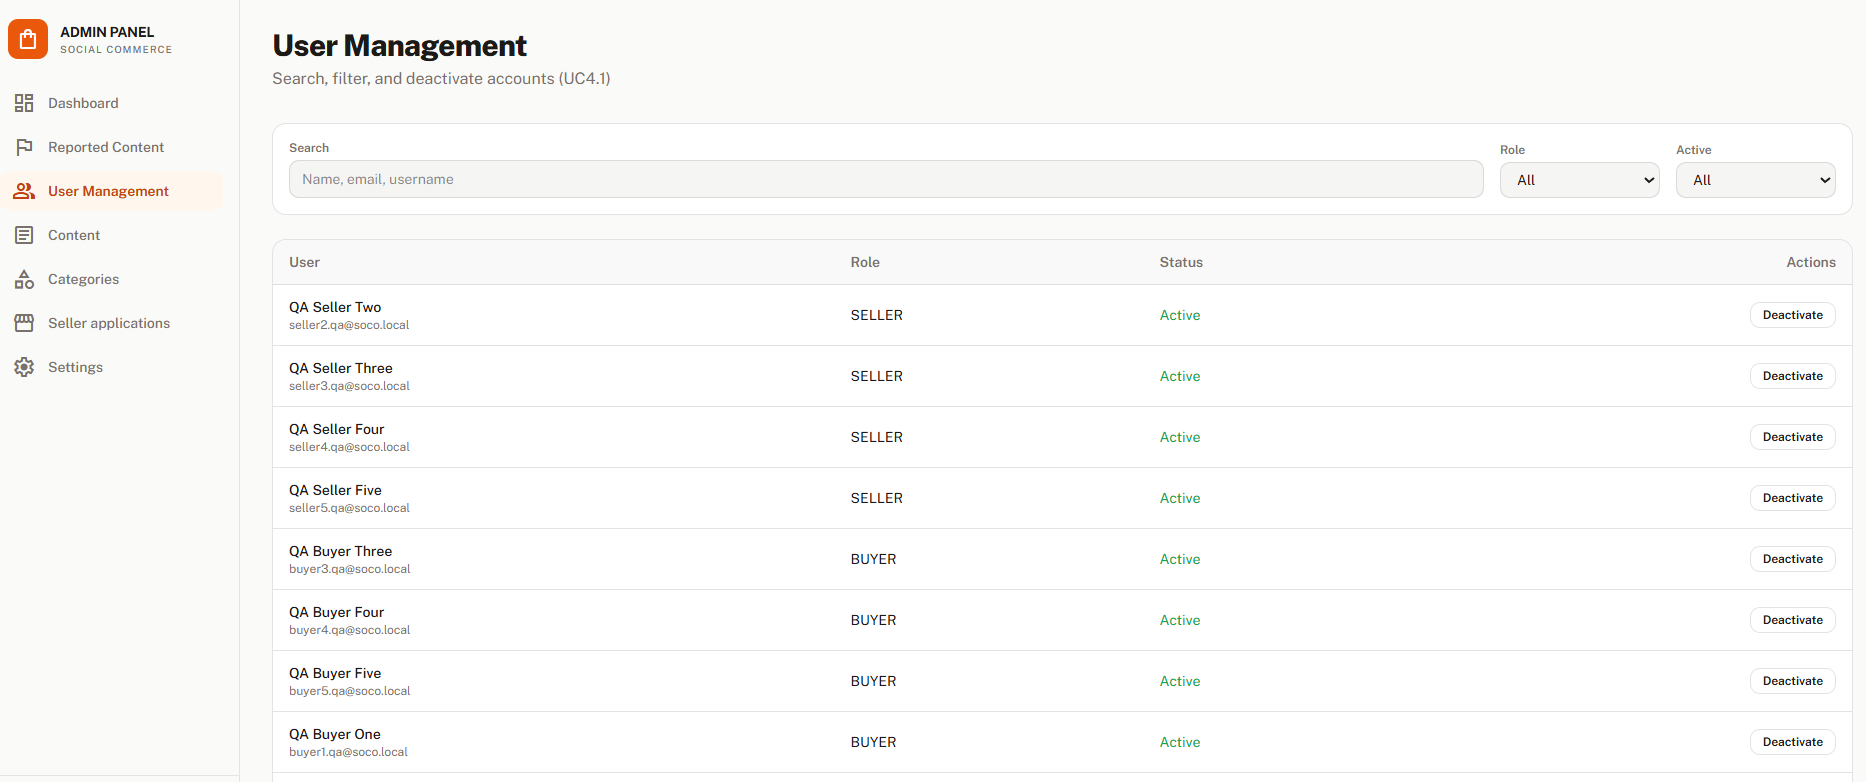
\includegraphics[width=\textwidth]{Images/UI/module4/user-management.png}
\caption{Giao diện quản lý người dùng}
\label{fig:module4-user-management}
\end{figure}

\subsubsection{Trang Quản lý Nội dung}

Trang quản lý nội dung cho phép quản trị viên theo dõi và kiểm duyệt các bài đăng và sản phẩm được đăng tải trên nền tảng. Hệ thống hỗ trợ xem nhanh nội dung, thông tin người đăng và thời gian đăng tải nhằm phục vụ cho quá trình kiểm duyệt nội dung.

Quản trị viên có thể thực hiện các hành động như xóa nội dung vi phạm hoặc xử lý các bài đăng không phù hợp với chính sách của hệ thống.

\begin{figure}[H]
\centering
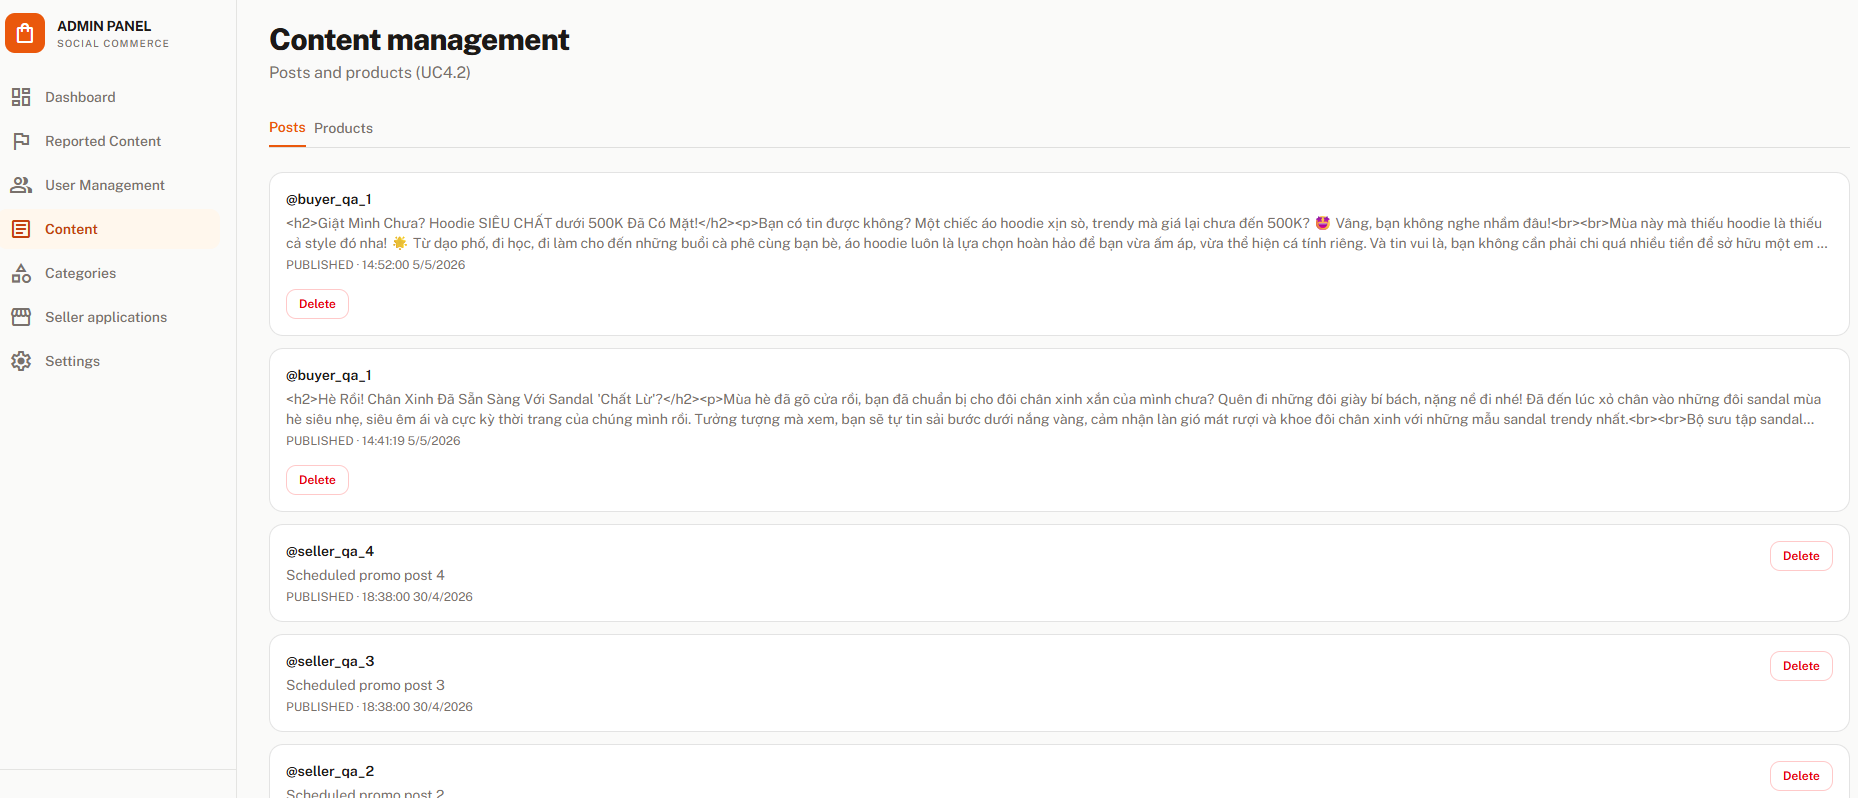
\includegraphics[width=\textwidth]{Images/UI/module4/content-management.png}
\caption{Giao diện quản lý nội dung}
\label{fig:module4-content-management}
\end{figure}

\subsubsection{Trang Quản lý Danh mục}

Trang quản lý danh mục hỗ trợ quản trị viên quản lý các danh mục sản phẩm trong marketplace. Hệ thống cho phép tạo mới, chỉnh sửa, kích hoạt hoặc vô hiệu hóa danh mục sản phẩm trực tiếp từ giao diện quản trị.

Ngoài ra, hệ thống còn hỗ trợ quản lý cấu trúc danh mục cha – con nhằm giúp tổ chức dữ liệu sản phẩm một cách trực quan và dễ quản lý hơn.

\begin{figure}[H]
\centering
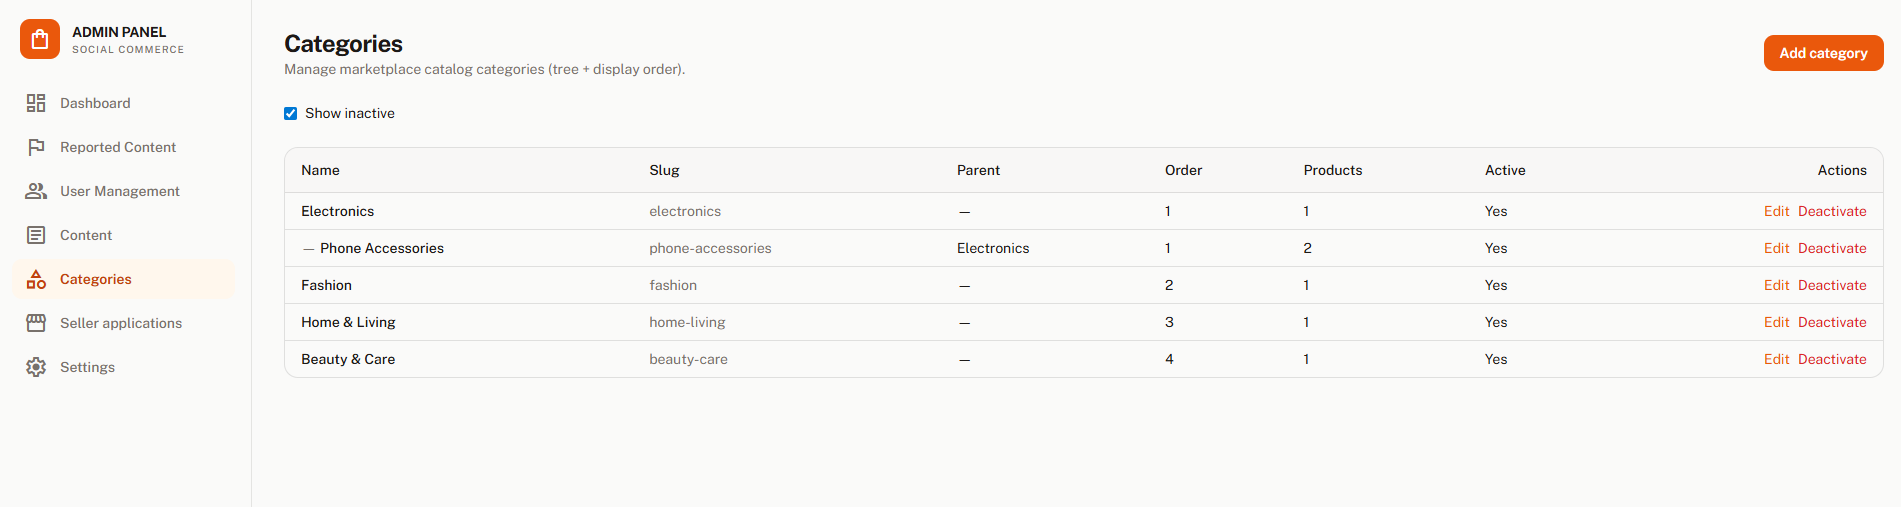
\includegraphics[width=\textwidth]{Images/UI/module4/category-management.png}
\caption{Giao diện quản lý danh mục sản phẩm}
\label{fig:module4-category-management}
\end{figure}

\subsubsection{Trang Xử lý Báo cáo}

Trang xử lý báo cáo hỗ trợ quản trị viên tiếp nhận và xử lý các báo cáo vi phạm phát sinh trên nền tảng. Hệ thống hiển thị danh sách các báo cáo liên quan đến bài đăng, sản phẩm hoặc tài khoản người dùng nhằm hỗ trợ kiểm duyệt nội dung và đảm bảo môi trường hoạt động an toàn.

Quản trị viên có thể xem chi tiết nội dung báo cáo, theo dõi trạng thái xử lý và thực hiện các hành động phù hợp như cảnh báo, ẩn nội dung hoặc khóa tài khoản vi phạm tùy theo mức độ của vấn đề được báo cáo.

\begin{figure}[H]
\centering
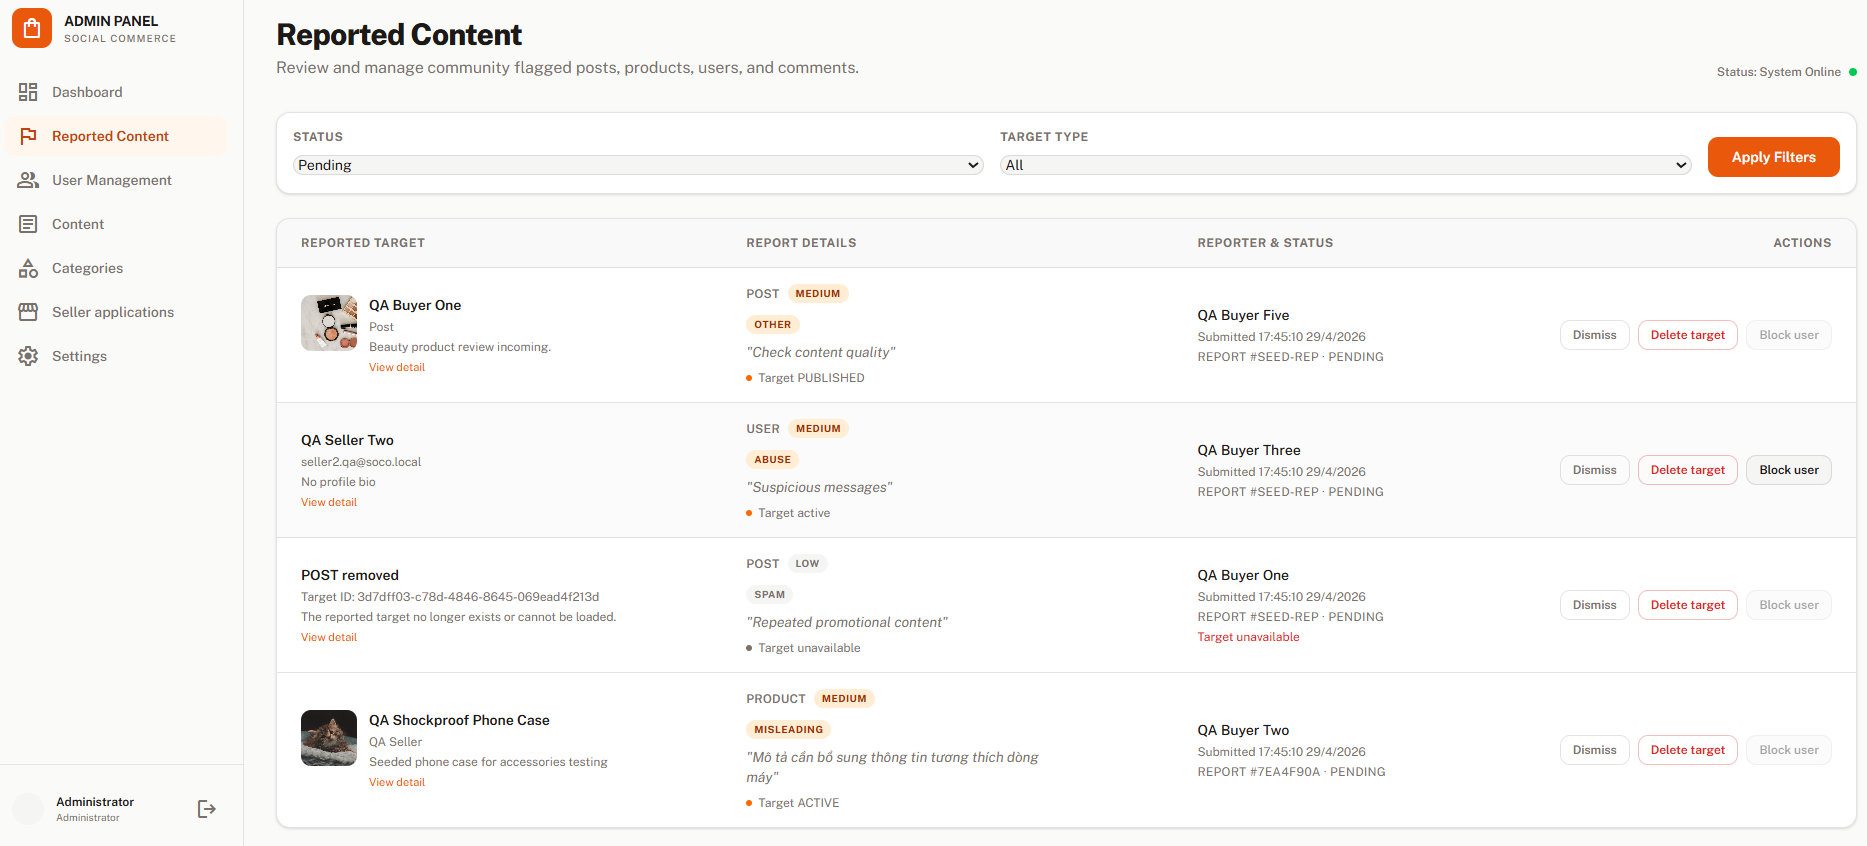
\includegraphics[width=\textwidth]{Images/UI/module4/report-management.png}
\caption{Giao diện xử lý báo cáo vi phạm}
\label{fig:module4-report-management}
\end{figure}



\section{Module 6: Quản lý Bài đăng Đã lên lịch}

Module quản lý bài đăng đã lên lịch hỗ trợ người dùng theo dõi và quản lý các bài viết được thiết lập đăng tải trong tương lai. Chức năng này được tích hợp trực tiếp với giao diện tạo bài đăng và AI Creative Studio nhằm hỗ trợ quá trình xây dựng nội dung và quản lý lịch đăng bài trên nền tảng.

\subsubsection{Trang Quản lý Bài đăng Đã lên lịch}

Trang quản lý bài đăng đã lên lịch hiển thị danh sách các bài viết đang chờ đăng tải và các bài viết đã được xuất bản trên hệ thống. Người dùng có thể xem nhanh nội dung bài viết, trạng thái bài đăng, thời gian đăng dự kiến và các thống kê liên quan trực tiếp từ giao diện quản lý.

Hệ thống hỗ trợ chỉnh sửa nội dung bài viết, thay đổi thời gian đăng hoặc hủy lịch đăng đối với các bài viết chưa được xuất bản. Ngoài ra, giao diện còn hiển thị các thống kê nhanh như số lượng bài viết sắp đăng, bài viết đã đăng và hoạt động đăng bài trong tuần nhằm hỗ trợ người dùng quản lý nội dung hiệu quả hơn.

\begin{figure}[H]
\centering
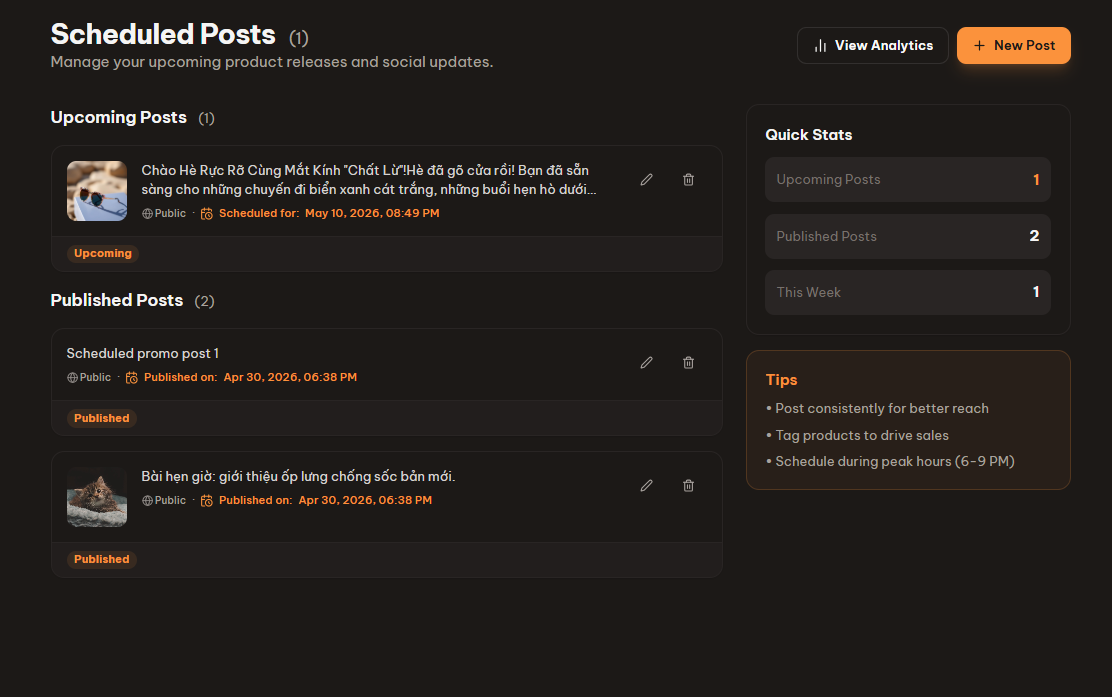
\includegraphics[width=\textwidth]{Images/UI/module6/scheduled-posts.png}
\caption{Giao diện quản lý bài đăng đã lên lịch}
\label{fig:module6-scheduled-posts}
\end{figure}

Người dùng cũng có thể chỉnh sửa bài đăng đã lên lịch trực tiếp thông qua giao diện chỉnh sửa bài viết. Hệ thống hỗ trợ thay đổi nội dung bài đăng, cấu hình AI Creative Lab và cập nhật thời gian đăng bài thông qua giao diện lịch trực quan.

\begin{figure}[H]
\centering
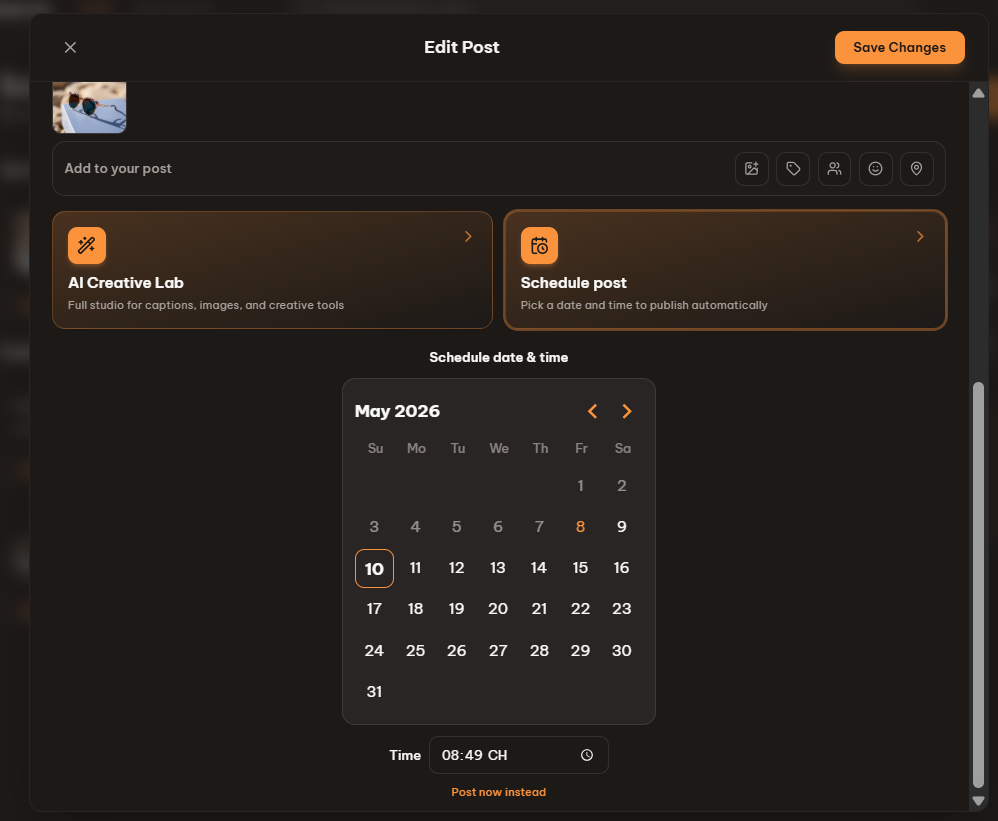
\includegraphics[width=\textwidth]{Images/UI/module6/edit-scheduled-post.png}
\caption{Giao diện chỉnh sửa bài đăng đã lên lịch}
\label{fig:module6-edit-scheduled-post}
\end{figure}


\section{Module 7: Hệ thống Thông báo}

Module thông báo hỗ trợ người dùng theo dõi các hoạt động và sự kiện mới phát sinh trên nền tảng Social Commerce. Hệ thống thông báo được xây dựng nhằm tăng khả năng tương tác giữa người dùng, đồng thời hỗ trợ cập nhật nhanh các hoạt động liên quan đến bài đăng, tin nhắn, đơn hàng và các sự kiện hệ thống.

\subsubsection{Trang Thông báo}

Trang thông báo hiển thị danh sách các thông báo phát sinh trong quá trình sử dụng hệ thống. Các thông báo được phân loại theo từng nhóm chức năng như tương tác bài viết, hoạt động thương mại, tin nhắn và thông báo hệ thống nhằm giúp người dùng dễ dàng theo dõi nội dung quan trọng.

Người dùng có thể xem trạng thái thông báo, đánh dấu đã đọc hoặc truy cập trực tiếp đến nội dung liên quan từ giao diện thông báo. Hệ thống đồng thời hỗ trợ cập nhật dữ liệu động nhằm đảm bảo các thông báo mới được hiển thị nhanh chóng trên nền tảng.

\begin{figure}[H]
\centering
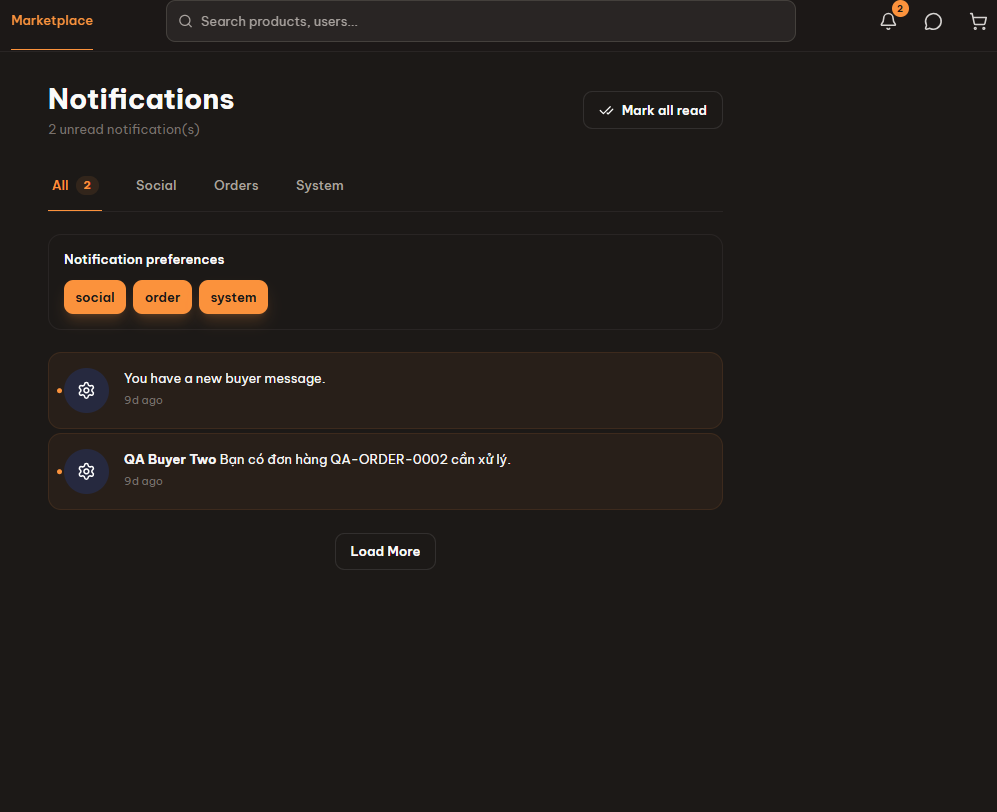
\includegraphics[width=\textwidth]{Images/UI/module7/notifications-page.png}
\caption{Giao diện trang thông báo}
\label{fig:module7-notifications-page}
\end{figure}

\subsubsection{Component Thông báo Real-time}

Hệ thống hỗ trợ thông báo real-time nhằm cập nhật nhanh các sự kiện mới như tin nhắn, tương tác bài viết hoặc cập nhật đơn hàng mà không cần tải lại trang. Các thông báo sẽ hiển thị dưới dạng popup trực tiếp trên giao diện người dùng nhằm đảm bảo trải nghiệm sử dụng liền mạch và thuận tiện hơn.

Người dùng có thể đóng nhanh thông báo hoặc truy cập trực tiếp đến nội dung liên quan từ popup thông báo real-time.

\begin{figure}[H]
\centering
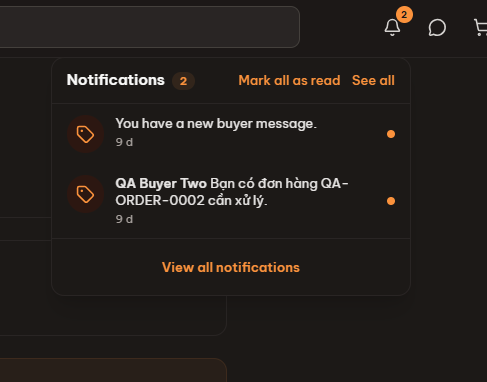
\includegraphics[width=0.6\textwidth]{Images/UI/module7/realtime-notification-popup.png}
\caption{Component thông báo real-time}
\label{fig:module7-realtime-notification-popup}
\end{figure}





\clearpage
\chapter{Kiểm thử}

Chương này trình bày quá trình kiểm thử hệ thống Social Commerce sau giai đoạn hiện thực. Mục tiêu của kiểm thử là xác nhận các chức năng chính hoạt động đúng theo yêu cầu, API trả về dữ liệu nhất quán, các luồng phân quyền được bảo vệ hợp lý và giao diện người dùng đạt mức phản hồi chấp nhận được trong môi trường kiểm thử.

Phạm vi kiểm thử tập trung vào ba nhóm chính:

\begin{itemize}
    \item Kiểm thử API bằng Postman đối với core API và admin API.
    \item Kiểm thử luồng chức năng thông qua các kịch bản người dùng (user), seller và admin.
    \item Kiểm thử hiệu suất giao diện bằng Chrome DevTools và Lighthouse.
\end{itemize}

\section{Công cụ kiểm thử}

\subsection{Công cụ hỗ trợ kiểm thử Postman}

Postman được sử dụng làm công cụ chính để kiểm thử API vì phù hợp với hệ thống backend được xây dựng theo mô hình REST API. Công cụ này hỗ trợ tạo collection endpoint, cấu hình biến môi trường, lưu token sau khi đăng nhập và kiểm tra response tự động bằng script.

Trong quá trình kiểm thử, nhóm cấu hình các biến môi trường chính như sau:

\begin{table}[H]
\centering
\caption{Các biến môi trường sử dụng trong Postman}
\begin{tabularx}{\textwidth}{|p{0.28\textwidth}|X|}
\hline
\textbf{Biến môi trường} & \textbf{Ý nghĩa} \\ \hline
\texttt{baseUrl} & URL của core backend API, ví dụ \texttt{http://localhost:5000/api}. \\ \hline
\texttt{adminBaseUrl} & URL của admin backend API, ví dụ \texttt{http://localhost:5001/api}. \\ \hline
\texttt{accessToken} & JWT token của buyer/seller sau khi đăng nhập thành công. \\ \hline
\texttt{adminToken} & JWT token của admin sau khi đăng nhập admin. \\ \hline
\texttt{userId}, \texttt{productId}, \texttt{postId}, \texttt{orderId} & Các ID được lấy từ response trước đó để dùng cho các request phụ thuộc. \\ \hline
\end{tabularx}
\end{table}

Các nhóm API được đưa vào Postman collection gồm:

\begin{itemize}
    \item \textbf{Authentication}: đăng ký, xác thực email, đăng nhập, đăng xuất, quên mật khẩu, reset password và 2FA.
    \item \textbf{User/Profile}: xem và cập nhật hồ sơ, follow/unfollow, tìm kiếm người dùng.
    \item \textbf{Social}: bài viết, feed, like, comment, saved items, báo cáo vi phạm.
    \item \textbf{Commerce}: sản phẩm, danh mục, giỏ hàng, checkout, đơn hàng và đánh giá.
    \item \textbf{Seller}: đăng ký seller, trạng thái hồ sơ, sản phẩm seller, biến thể sản phẩm và đơn bán.
    \item \textbf{Messaging/Notification}: conversation, message, notification và notification preferences.
    \item \textbf{AI/Scheduled posts}: tạo nội dung AI, lưu lịch sử AI, tư vấn mua sắm qua AI chatbox, tạo và quản lý bài viết đã lên lịch.
    \item \textbf{Admin}: đăng nhập admin, dashboard, users, posts, products, reports, seller applications và sensitive change requests.
\end{itemize}

\section{Kiểm thử API}

\subsection{Cách thực hiện}

Quy trình kiểm thử API được thực hiện theo các bước sau:

\begin{enumerate}
    \item \textbf{Chuẩn bị dữ liệu}: tạo các tài khoản kiểm thử gồm buyer, seller và admin; seed dữ liệu sản phẩm, bài viết, danh mục, đơn hàng và báo cáo vi phạm.
    \item \textbf{Đăng nhập và lưu token}: gọi API đăng nhập, lưu JWT vào biến môi trường Postman để dùng cho các request yêu cầu xác thực.
    \item \textbf{Kiểm thử request hợp lệ}: gửi request với dữ liệu đúng và kiểm tra HTTP status code, cấu trúc response, message và dữ liệu trả về.
    \item \textbf{Kiểm thử request không hợp lệ}: gửi dữ liệu thiếu field, sai định dạng, token không hợp lệ hoặc sai role để kiểm tra validation và authorization.
    \item \textbf{Kiểm thử dữ liệu phụ thuộc}: với các luồng như tạo sản phẩm, thêm giỏ hàng, checkout, tạo review, nhóm kiểm tra thứ tự request và dữ liệu sinh ra từ bước trước.
    \item \textbf{Đối chiếu database}: với các chức năng ghi dữ liệu quan trọng, kiểm tra lại dữ liệu trong PostgreSQL thông qua Prisma Studio hoặc database client.
    \item \textbf{Kiểm tra side effect}: xác nhận các side effect như tăng số lượng like/comment, tạo notification, cập nhật trạng thái đơn hàng hoặc lưu lịch sử AI.
\end{enumerate}

Các tiêu chí đánh giá kết quả gồm:

\begin{itemize}
    \item API trả đúng status code: \texttt{200}, \texttt{201}, \texttt{400}, \texttt{401}, \texttt{403}, \texttt{404} tùy tình huống.
    \item Response có cấu trúc thống nhất, thường gồm \texttt{success}, \texttt{message}, \texttt{data} và \texttt{pagination} nếu là danh sách.
    \item Các endpoint yêu cầu đăng nhập phải từ chối request không có token hoặc token sai.
    \item Các endpoint dành cho seller/admin phải kiểm tra đúng quyền truy cập.
    \item Dữ liệu tạo mới/cập nhật/xóa mềm phải phản ánh đúng trong database.
\end{itemize}

\subsection{Kết quả test case tổng hợp}

Bảng sau tổng hợp kết quả kiểm thử theo từng nhóm chức năng chính của hệ thống.

\begin{longtable}{|>{\raggedright\arraybackslash}p{0.15\textwidth}|p{0.24\textwidth}|p{0.36\textwidth}|p{0.14\textwidth}|}
\caption{Kết quả kiểm thử API tổng hợp} \\
\hline
\textbf{Mã nhóm} & \textbf{Nhóm chức năng} & \textbf{Nội dung kiểm thử chính} & \textbf{Kết quả} \\ \hline
\endfirsthead
\hline
\textbf{Mã nhóm} & \textbf{Nhóm chức năng} & \textbf{Nội dung kiểm thử chính} & \textbf{Kết quả} \\ \hline
\endhead
AUTH & Xác thực tài khoản & Đăng ký, xác thực email, đăng nhập, đăng xuất, quên mật khẩu, reset password, bật/tắt 2FA. & Đạt \\ \hline
USER & Hồ sơ và quan hệ người dùng & Xem/cập nhật hồ sơ, tìm kiếm user, follow/unfollow, quyền truy cập hồ sơ. & Đạt \\ \hline
POST & Bài viết và feed & Tạo bài viết, gắn nhiều sản phẩm qua \texttt{productTags}, xem feed, like, comment, share, xóa bài viết. & Đạt \\ \hline
GROUP & Nhóm cộng đồng & Tạo nhóm, tham gia/rời nhóm, duyệt yêu cầu tham gia, bài viết trong nhóm, invite. & Đạt \\ \hline
PRODUCT & Sản phẩm và marketplace & Tạo/sửa/xóa mềm/khôi phục sản phẩm, ảnh sản phẩm, biến thể, danh mục, tìm kiếm và lọc sản phẩm. & Đạt \\ \hline
CART & Giỏ hàng & Thêm sản phẩm vào giỏ, cập nhật số lượng, xóa item, lấy tổng số item. & Đạt \\ \hline
ORDER & Đơn hàng & Checkout, xem đơn mua/bán, cập nhật trạng thái, hủy đơn, yêu cầu hoàn tiền giả lập. & Đạt \\ \hline
REVIEW & Đánh giá sản phẩm & Tạo review sau mua, xem review, seller phản hồi review. & Đạt \\ \hline
MSG & Tin nhắn và thông báo & Tạo conversation, gửi tin nhắn, đánh dấu đã đọc, lấy notification, cập nhật preferences. & Đạt \\ \hline
AI & AI, chatbox và bài lên lịch & Tạo text/image content, lưu AI history, tư vấn mua sắm qua AI chatbox, tạo/sửa/xóa/publish scheduled post. & Đạt \\ \hline
REPORT & Báo cáo vi phạm & Buyer/seller tạo report cho post, comment, product, user; admin xem và xử lý report. & Đạt \\ \hline
ADMIN & Quản trị hệ thống & Đăng nhập admin, dashboard, quản lý users, posts, products, categories, seller applications. & Đạt \\ \hline
\end{longtable}

\subsection{Kịch bản và kết quả kiểm thử}

Phần này mô tả các kịch bản kiểm thử tiêu biểu đã được thực hiện trên Postman và giao diện web. Các kịch bản được chọn để bao phủ các luồng nghiệp vụ quan trọng và các trường hợp phân quyền thường gặp.

\newcommand{\apiendpoint}[1]{\begingroup\ttfamily\scriptsize\seqsplit{#1}\endgroup}
{\scriptsize
\setlength{\tabcolsep}{1.5pt}
\renewcommand{\arraystretch}{1.12}
\begin{longtable}{|>{\centering\arraybackslash}p{0.045\textwidth}|>{\raggedright\arraybackslash}p{0.09\textwidth}|>{\raggedright\arraybackslash}p{0.20\textwidth}|>{\raggedright\arraybackslash}p{0.22\textwidth}|>{\raggedright\arraybackslash}p{0.325\textwidth}|>{\centering\arraybackslash}p{0.055\textwidth}|}
\caption{Kịch bản kiểm thử chức năng và API chi tiết} \\
\hline
\textbf{STT} & \textbf{Nhóm API} & \textbf{Tên API} & \textbf{Testcase thực hiện} & \textbf{Kết quả mong muốn} & \textbf{Kết quả} \\ \hline
\endfirsthead
\hline
\textbf{STT} & \textbf{Nhóm API} & \textbf{Tên API} & \textbf{Testcase thực hiện} & \textbf{Kết quả mong muốn} & \textbf{Kết quả} \\ \hline
\endhead
1 & auth & \apiendpoint{POST /api/auth/register} & \texttt{TC\_AUTH\_01} - Register success for buyer & Status code \texttt{201}; response có \texttt{success=true}; user được tạo ở trạng thái chờ xác thực email. & PASS \\ \hline
2 & auth & \apiendpoint{POST /api/auth/register} & \texttt{TC\_AUTH\_02} - Register success for seller account & Status code \texttt{201}; user được tạo với role phù hợp; gửi OTP xác thực email. & PASS \\ \hline
3 & auth & \apiendpoint{POST /api/auth/register} & \texttt{TC\_AUTH\_03} - Register fail duplicate email & Status code \texttt{400}/\texttt{409}; message thông báo email đã được sử dụng. & PASS \\ \hline
4 & auth & \apiendpoint{POST /api/auth/register} & \texttt{TC\_AUTH\_04} - Register fail duplicate username & Status code \texttt{400}/\texttt{409}; message thông báo username đã được sử dụng. & PASS \\ \hline
5 & auth & \apiendpoint{POST /api/auth/register} & \texttt{TC\_AUTH\_05} - Register fail missing required fields & Status code \texttt{400}; response có validation error; không tạo user. & PASS \\ \hline
6 & auth & \apiendpoint{POST /api/auth/register} & \texttt{TC\_AUTH\_06} - Register fail weak password & Status code \texttt{400}; message yêu cầu password hợp lệ. & PASS \\ \hline
7 & auth & \apiendpoint{POST /api/auth/verify-email} & \texttt{TC\_AUTH\_07} - Verify email success & Status code \texttt{200}; user chuyển sang trạng thái verified. & PASS \\ \hline
8 & auth & \apiendpoint{POST /api/auth/verify-email} & \texttt{TC\_AUTH\_08} - Verify email fail invalid OTP & Status code \texttt{400}; không xác thực tài khoản. & PASS \\ \hline
9 & auth & \apiendpoint{POST /api/auth/resend-verification} & \texttt{TC\_AUTH\_09} - Resend verification success & Status code \texttt{200}; hệ thống gửi lại OTP xác thực email. & PASS \\ \hline
10 & auth & \apiendpoint{POST /api/auth/login} & \texttt{TC\_AUTH\_10} - Login success for buyer & Status code \texttt{200}; trả access token và thông tin buyer. & PASS \\ \hline
11 & auth & \apiendpoint{POST /api/auth/login} & \texttt{TC\_AUTH\_11} - Login success for seller & Status code \texttt{200}; trả access token và thông tin seller. & PASS \\ \hline
12 & auth & \apiendpoint{POST /api/auth/login} & \texttt{TC\_AUTH\_12} - Login fail wrong password & Status code \texttt{401}; không trả token. & PASS \\ \hline
13 & auth & \apiendpoint{POST /api/auth/login} & \texttt{TC\_AUTH\_13} - Login fail unverified account & Status code \texttt{403}; response trả thông tin cần xác thực email. & PASS \\ \hline
14 & auth & \apiendpoint{POST /api/auth/login} & \texttt{TC\_AUTH\_14} - Login requires 2FA & Status code \texttt{200}; response có \texttt{requires2FA=true} và \texttt{tempToken}. & PASS \\ \hline
15 & auth & \apiendpoint{POST /api/auth/verify-2fa} & \texttt{TC\_AUTH\_15} - Verify 2FA success & Status code \texttt{200}; trả access token chính thức sau khi OTP đúng. & PASS \\ \hline
16 & auth & \apiendpoint{POST /api/auth/verify-2fa} & \texttt{TC\_AUTH\_16} - Verify 2FA fail wrong OTP & Status code \texttt{400}/\texttt{401}; không cấp access token. & PASS \\ \hline
17 & auth & \apiendpoint{GET /api/auth/me} & \texttt{TC\_AUTH\_17} - Get current user success & Status code \texttt{200}; response trả đúng user theo JWT. & PASS \\ \hline
18 & auth & \apiendpoint{GET /api/auth/me} & \texttt{TC\_AUTH\_18} - Get current user without token & Status code \texttt{401}; không trả thông tin user. & PASS \\ \hline
19 & auth & \apiendpoint{PUT /api/auth/profile} & \texttt{TC\_AUTH\_19} - Update profile success & Status code \texttt{200}; profile được cập nhật đúng dữ liệu gửi lên. & PASS \\ \hline
20 & auth & \apiendpoint{PUT /api/auth/password} & \texttt{TC\_AUTH\_20} - Change password success & Status code \texttt{200}; password mới dùng được khi đăng nhập lại. & PASS \\ \hline
21 & auth & \apiendpoint{PUT /api/auth/password} & \texttt{TC\_AUTH\_21} - Change password fail wrong current password & Status code \texttt{400}/\texttt{401}; password không bị thay đổi. & PASS \\ \hline
22 & auth & \apiendpoint{POST /api/auth/2fa/enable} & \texttt{TC\_AUTH\_22} - Enable 2FA send OTP & Status code \texttt{200}; OTP được gửi tới email. & PASS \\ \hline
23 & auth & \apiendpoint{POST /api/auth/2fa/confirm} & \texttt{TC\_AUTH\_23} - Confirm enable 2FA success & Status code \texttt{200}; \texttt{isEnabled=true}. & PASS \\ \hline
24 & auth & \apiendpoint{POST /api/auth/2fa/disable} & \texttt{TC\_AUTH\_24} - Disable 2FA success & Status code \texttt{200}; 2FA được tắt sau khi nhập đúng password. & PASS \\ \hline
25 & auth & \apiendpoint{POST /api/auth/2fa/disable} & \texttt{TC\_AUTH\_25} - Disable 2FA fail wrong password & Status code \texttt{400}/\texttt{401}; 2FA vẫn bật. & PASS \\ \hline

26 & user & \apiendpoint{GET /api/users/me} & \texttt{TC\_USER\_01} - Get my profile success & Status code \texttt{200}; trả profile của user hiện tại. & PASS \\ \hline
27 & user & \apiendpoint{PUT /api/users/me} & \texttt{TC\_USER\_02} - Update my profile success & Status code \texttt{200}; dữ liệu profile được cập nhật. & PASS \\ \hline
28 & user & \apiendpoint{GET /api/users/search} & \texttt{TC\_USER\_03} - Search users success & Status code \texttt{200}; response trả danh sách user phù hợp keyword. & PASS \\ \hline
29 & user & \apiendpoint{POST /api/users/:userId/follow} & \texttt{TC\_USER\_04} - Follow user success & Status code \texttt{200}; tạo quan hệ follow và notification. & PASS \\ \hline
30 & user & \apiendpoint{POST /api/users/:userId/follow} & \texttt{TC\_USER\_05} - Follow self fail & Status code \texttt{400}; không tạo quan hệ follow. & PASS \\ \hline
31 & user & \apiendpoint{DELETE /api/users/:userId/follow} & \texttt{TC\_USER\_06} - Unfollow success & Status code \texttt{200}; quan hệ follow bị xóa. & PASS \\ \hline
32 & user & \apiendpoint{GET /api/users/:userId} & \texttt{TC\_USER\_07} - Get public profile success & Status code \texttt{200}; trả public profile. & PASS \\ \hline
33 & user & \apiendpoint{GET /api/users/:userId} & \texttt{TC\_USER\_08} - Get nonexistent user & Status code \texttt{404}; response có message phù hợp. & PASS \\ \hline

34 & post & \apiendpoint{GET /api/posts} & \texttt{TC\_POST\_01} - Get public posts success & Status code \texttt{200}; response có data và pagination. & PASS \\ \hline
35 & post & \apiendpoint{GET /api/posts/feed} & \texttt{TC\_POST\_02} - Get personalized feed success & Status code \texttt{200}; trả feed theo user đã đăng nhập. & PASS \\ \hline
36 & post & \apiendpoint{GET /api/posts/feed} & \texttt{TC\_POST\_03} - Get feed without token & Status code \texttt{401}; không trả personalized feed. & PASS \\ \hline
37 & post & \apiendpoint{POST /api/posts} & \texttt{TC\_POST\_04} - Create post success & Status code \texttt{201}; bài viết được lưu vào database. & PASS \\ \hline
38 & post & \apiendpoint{POST /api/posts} & \texttt{TC\_POST\_05} - Create post with multiple product tags & Status code \texttt{201}; response có \texttt{taggedProducts}; tạo bản ghi \textit{post\_product\_tags}. & PASS \\ \hline
39 & post & \apiendpoint{POST /api/posts} & \texttt{TC\_POST\_06} - Create post fail invalid productTags & Status code \texttt{400}; không tạo bài viết/tag. & PASS \\ \hline
40 & post & \apiendpoint{PUT /api/posts/:id} & \texttt{TC\_POST\_07} - Update own post success & Status code \texttt{200}; nội dung bài viết được cập nhật. & PASS \\ \hline
41 & post & \apiendpoint{PUT /api/posts/:id} & \texttt{TC\_POST\_08} - Update another user's post fail & Status code \texttt{403}; bài viết không bị thay đổi. & PASS \\ \hline
42 & post & \apiendpoint{DELETE /api/posts/:id} & \texttt{TC\_POST\_09} - Delete own post success & Status code \texttt{200}; bài viết bị xóa/ẩn khỏi danh sách. & PASS \\ \hline
43 & post & \apiendpoint{GET /api/posts/:id} & \texttt{TC\_POST\_10} - Get nonexistent post & Status code \texttt{404}; message \texttt{Post not found}. & PASS \\ \hline
44 & post & \apiendpoint{POST /api/posts/:id/like} & \texttt{TC\_POST\_11} - Like/unlike success & Status code \texttt{200}; trạng thái like được toggle. & PASS \\ \hline
45 & post & \apiendpoint{POST /api/posts/:id/comments} & \texttt{TC\_POST\_12} - Add comment success & Status code \texttt{201}/\texttt{200}; comment được lưu. & PASS \\ \hline
46 & post & \apiendpoint{POST /api/posts/:id/comments} & \texttt{TC\_POST\_13} - Add empty comment fail & Status code \texttt{400}; không tạo comment. & PASS \\ \hline
47 & post & \apiendpoint{GET /api/posts/:id/comments} & \texttt{TC\_POST\_14} - Get comments success & Status code \texttt{200}; trả danh sách comment theo phân trang. & PASS \\ \hline

48 & product & \apiendpoint{GET /api/products} & \texttt{TC\_PROD\_01} - Get product list success & Status code \texttt{200}; response có data và pagination. & PASS \\ \hline
49 & product & \apiendpoint{GET /api/products?search=...} & \texttt{TC\_PROD\_02} - Search/filter products success & Status code \texttt{200}; danh sách phản ánh keyword/filter. & PASS \\ \hline
50 & product & \apiendpoint{GET /api/products/:id} & \texttt{TC\_PROD\_03} - Get product detail success & Status code \texttt{200}; trả thông tin sản phẩm, ảnh, variant, seller. & PASS \\ \hline
51 & product & \apiendpoint{GET /api/products/:id} & \texttt{TC\_PROD\_04} - Product not found & Status code \texttt{404}; message \texttt{Product not found}. & PASS \\ \hline
52 & product & \apiendpoint{POST /api/products} & \texttt{TC\_PROD\_05} - Seller create product success & Status code \texttt{201}; sản phẩm thuộc seller hiện tại. & PASS \\ \hline
53 & product & \apiendpoint{POST /api/products} & \texttt{TC\_PROD\_06} - Buyer create product fail & Status code \texttt{403}; không tạo sản phẩm. & PASS \\ \hline
54 & product & \apiendpoint{POST /api/products} & \texttt{TC\_PROD\_07} - Create product fail missing title/price & Status code \texttt{400}; validation error. & PASS \\ \hline
55 & product & \apiendpoint{PUT /api/products/:id} & \texttt{TC\_PROD\_08} - Seller update own product success & Status code \texttt{200}; sản phẩm được cập nhật. & PASS \\ \hline
56 & product & \apiendpoint{PUT /api/products/:id} & \texttt{TC\_PROD\_09} - Seller update other seller product fail & Status code \texttt{403}/\texttt{404}; không cập nhật dữ liệu. & PASS \\ \hline
57 & product & \apiendpoint{DELETE /api/products/:id} & \texttt{TC\_PROD\_10} - Soft delete product success & Status code \texttt{200}; sản phẩm chuyển trạng thái xóa mềm. & PASS \\ \hline
58 & product & \apiendpoint{POST /api/products/:id/restore} & \texttt{TC\_PROD\_11} - Restore product success & Status code \texttt{200}; sản phẩm được khôi phục. & PASS \\ \hline
59 & product & \apiendpoint{POST /api/products/:id/publish} & \texttt{TC\_PROD\_12} - Publish product success & Status code \texttt{200}; sản phẩm chuyển trạng thái hiển thị. & PASS \\ \hline
60 & product & \apiendpoint{POST /api/products/:id/images} & \texttt{TC\_PROD\_13} - Add images success & Status code \texttt{200}; ảnh sản phẩm được thêm. & PASS \\ \hline
61 & product & \apiendpoint{POST /api/products/:id/images} & \texttt{TC\_PROD\_14} - Add images fail invalid body & Status code \texttt{400}; không thêm ảnh. & PASS \\ \hline
62 & product & \apiendpoint{POST /api/products/seller/me/:productId/variants} & \texttt{TC\_PROD\_15} - Create variant success & Status code \texttt{201}/\texttt{200}; variant được tạo cho sản phẩm của seller. & PASS \\ \hline
63 & product & \apiendpoint{POST /api/products/seller/me/:productId/variants} & \texttt{TC\_PROD\_16} - Create variant fail invalid stock/price & Status code \texttt{400}; không tạo variant. & PASS \\ \hline

64 & cart & \apiendpoint{GET /api/cart} & \texttt{TC\_CART\_01} - Get cart success & Status code \texttt{200}; trả cart, items, subtotal. & PASS \\ \hline
65 & cart & \apiendpoint{GET /api/cart} & \texttt{TC\_CART\_02} - Get cart without token & Status code \texttt{401}; không trả cart. & PASS \\ \hline
66 & cart & \apiendpoint{POST /api/cart/items} & \texttt{TC\_CART\_03} - Add item success & Status code \texttt{201}/\texttt{200}; cart item được tạo/cập nhật. & PASS \\ \hline
67 & cart & \apiendpoint{POST /api/cart/items} & \texttt{TC\_CART\_04} - Add item fail quantity less than 1 & Status code \texttt{400}; cart không thay đổi. & PASS \\ \hline
68 & cart & \apiendpoint{POST /api/cart/items} & \texttt{TC\_CART\_05} - Add nonexistent product & Status code \texttt{404}; không tạo cart item. & PASS \\ \hline
69 & cart & \apiendpoint{PUT /api/cart/items/:itemId} & \texttt{TC\_CART\_06} - Update quantity success & Status code \texttt{200}; số lượng item được cập nhật. & PASS \\ \hline
70 & cart & \apiendpoint{PUT /api/cart/items/:itemId} & \texttt{TC\_CART\_07} - Update item not owned fail & Status code \texttt{403}; không cập nhật item. & PASS \\ \hline
71 & cart & \apiendpoint{DELETE /api/cart/items/:itemId} & \texttt{TC\_CART\_08} - Remove item success & Status code \texttt{200}; item bị xóa khỏi cart. & PASS \\ \hline
72 & cart & \apiendpoint{DELETE /api/cart} & \texttt{TC\_CART\_09} - Clear cart success & Status code \texttt{200}; cart không còn item. & PASS \\ \hline

73 & order & \apiendpoint{POST /api/orders} & \texttt{TC\_ORDER\_01} - Checkout success & Status code \texttt{201}; tạo order và order items. & PASS \\ \hline
74 & order & \apiendpoint{POST /api/orders} & \texttt{TC\_ORDER\_02} - Checkout fail empty cart & Status code \texttt{400}; không tạo order. & PASS \\ \hline
75 & order & \apiendpoint{POST /api/orders} & \texttt{TC\_ORDER\_03} - Checkout fail invalid shipping phone & Status code \texttt{400}; validation error. & PASS \\ \hline
76 & order & \apiendpoint{GET /api/orders/my/purchases} & \texttt{TC\_ORDER\_04} - Get buyer orders success & Status code \texttt{200}; trả danh sách đơn mua. & PASS \\ \hline
77 & order & \apiendpoint{GET /api/orders/my/sales} & \texttt{TC\_ORDER\_05} - Get seller sales success & Status code \texttt{200}; trả danh sách đơn bán liên quan seller. & PASS \\ \hline
78 & order & \apiendpoint{GET /api/orders/:orderId} & \texttt{TC\_ORDER\_06} - Get own order success & Status code \texttt{200}; trả chi tiết order. & PASS \\ \hline
79 & order & \apiendpoint{GET /api/orders/:orderId} & \texttt{TC\_ORDER\_07} - Get another user's order fail & Status code \texttt{403}; không lộ dữ liệu đơn hàng. & PASS \\ \hline
80 & order & \apiendpoint{PUT /api/orders/:orderId/status} & \texttt{TC\_ORDER\_08} - Seller update status success & Status code \texttt{200}; trạng thái đơn được cập nhật hợp lệ. & PASS \\ \hline
81 & order & \apiendpoint{PUT /api/orders/:orderId/status} & \texttt{TC\_ORDER\_09} - Invalid status transition fail & Status code \texttt{400}; trạng thái không đổi. & PASS \\ \hline
82 & order & \apiendpoint{POST /api/orders/:orderId/cancel} & \texttt{TC\_ORDER\_10} - Cancel pending order success & Status code \texttt{200}; order chuyển cancelled. & PASS \\ \hline
83 & order & \apiendpoint{POST /api/orders/:orderId/cancel} & \texttt{TC\_ORDER\_11} - Cancel delivered order fail & Status code \texttt{400}; order không bị hủy. & PASS \\ \hline
84 & order & \apiendpoint{POST /api/orders/:orderId/payment/confirm} & \texttt{TC\_ORDER\_12} - Confirm payment success & Status code \texttt{200}; paymentStatus được cập nhật. & PASS \\ \hline
85 & order & \apiendpoint{POST /api/orders/:orderId/refund-request} & \texttt{TC\_ORDER\_13} - Request refund success & Status code \texttt{200}; lưu yêu cầu hoàn tiền. & PASS \\ \hline
86 & order & \apiendpoint{POST /api/orders/:orderId/refund} & \texttt{TC\_ORDER\_14} - Seller process refund success & Status code \texttt{200}; trạng thái refund được xử lý. & PASS \\ \hline

87 & review & \apiendpoint{GET /api/reviews/product/:productId} & \texttt{TC\_REV\_01} - Get product reviews success & Status code \texttt{200}; trả danh sách review. & PASS \\ \hline
88 & review & \apiendpoint{POST /api/reviews} & \texttt{TC\_REV\_02} - Create review success & Status code \texttt{201}; review liên kết product/orderItem. & PASS \\ \hline
89 & review & \apiendpoint{POST /api/reviews} & \texttt{TC\_REV\_03} - Review without purchase fail & Status code \texttt{400}/\texttt{403}; không tạo review. & PASS \\ \hline
90 & review & \apiendpoint{POST /api/reviews/:reviewId/reply} & \texttt{TC\_REV\_04} - Seller response success & Status code \texttt{200}; seller response được lưu. & PASS \\ \hline
91 & review & \apiendpoint{POST /api/reviews/:reviewId/reply} & \texttt{TC\_REV\_05} - Non-owner seller response fail & Status code \texttt{403}; không cập nhật review. & PASS \\ \hline

92 & group & \apiendpoint{POST /api/groups} & \texttt{TC\_GROUP\_01} - Create group success & Status code \texttt{201}; group được tạo, creator là admin/owner của group. & PASS \\ \hline
93 & group & \apiendpoint{GET /api/groups} & \texttt{TC\_GROUP\_02} - Get groups success & Status code \texttt{200}; trả danh sách group theo filter. & PASS \\ \hline
94 & group & \apiendpoint{POST /api/groups/:groupId/join} & \texttt{TC\_GROUP\_03} - Join public group success & Status code \texttt{200}; tạo group member. & PASS \\ \hline
95 & group & \apiendpoint{POST /api/groups/:groupId/join} & \texttt{TC\_GROUP\_04} - Join private group creates request & Status code \texttt{200}/\texttt{201}; tạo join request pending. & PASS \\ \hline
96 & group & \apiendpoint{POST /api/groups/:groupId/requests/:requestId/approve} & \texttt{TC\_GROUP\_05} - Approve join request success & Status code \texttt{200}; request approved và user thành member. & PASS \\ \hline
97 & group & \apiendpoint{POST /api/groups/:groupId/posts} & \texttt{TC\_GROUP\_06} - Create group post success & Status code \texttt{201}; bài viết có \texttt{groupId}. & PASS \\ \hline
98 & group & \apiendpoint{POST /api/groups/:groupId/posts} & \texttt{TC\_GROUP\_07} - Non-member create group post fail & Status code \texttt{403}; không tạo bài viết. & PASS \\ \hline

99 & message & \apiendpoint{POST /api/messages/conversations} & \texttt{TC\_MSG\_01} - Create conversation success & Status code \texttt{200}/\texttt{201}; trả conversation hợp lệ. & PASS \\ \hline
100 & message & \apiendpoint{GET /api/messages/conversations} & \texttt{TC\_MSG\_02} - Get conversations success & Status code \texttt{200}; chỉ trả conversation của user hiện tại. & PASS \\ \hline
101 & message & \apiendpoint{POST /api/messages/conversations/:conversationId} & \texttt{TC\_MSG\_03} - Send message success & Status code \texttt{201}/\texttt{200}; message được lưu và emit realtime. & PASS \\ \hline
102 & message & \apiendpoint{POST /api/messages/conversations/:conversationId} & \texttt{TC\_MSG\_04} - Send empty message fail & Status code \texttt{400}; không tạo message. & PASS \\ \hline
103 & message & \apiendpoint{POST /api/messages/conversations/:conversationId} & \texttt{TC\_MSG\_05} - Non-participant send fail & Status code \texttt{403}; message không được lưu. & PASS \\ \hline
104 & message & \apiendpoint{PATCH /api/messages/conversations/:conversationId/read} & \texttt{TC\_MSG\_06} - Mark read success & Status code \texttt{200}; lastReadAt được cập nhật. & PASS \\ \hline

105 & notification & \apiendpoint{GET /api/notifications} & \texttt{TC\_NOTI\_01} - Get notifications success & Status code \texttt{200}; trả notification của user hiện tại. & PASS \\ \hline
106 & notification & \apiendpoint{PATCH /api/notifications/:id/read} & \texttt{TC\_NOTI\_02} - Mark notification as read success & Status code \texttt{200}; \texttt{isRead=true}. & PASS \\ \hline
107 & notification & \apiendpoint{PATCH /api/notifications/read-all} & \texttt{TC\_NOTI\_03} - Mark all as read success & Status code \texttt{200}; tất cả notification được đánh dấu đã đọc. & PASS \\ \hline
108 & notification & \apiendpoint{GET /api/notifications/preferences} & \texttt{TC\_NOTI\_04} - Get preferences success & Status code \texttt{200}; trả cấu hình notification. & PASS \\ \hline
109 & notification & \apiendpoint{PATCH /api/notifications/preferences} & \texttt{TC\_NOTI\_05} - Update preferences success & Status code \texttt{200}; preferences được lưu vào user settings. & PASS \\ \hline
110 & notification & \apiendpoint{DELETE /api/notifications/:id} & \texttt{TC\_NOTI\_06} - Delete notification success & Status code \texttt{200}; notification bị xóa. & PASS \\ \hline

111 & scheduled & \apiendpoint{POST /api/scheduled-posts} & \texttt{TC\_SCH\_01} - Schedule post success & Status code \texttt{201}; scheduled post ở trạng thái scheduled. & PASS \\ \hline
112 & scheduled & \apiendpoint{POST /api/scheduled-posts} & \texttt{TC\_SCH\_02} - Schedule post fail past time & Status code \texttt{400}; không tạo scheduled post. & PASS \\ \hline
113 & scheduled & \apiendpoint{GET /api/scheduled-posts} & \texttt{TC\_SCH\_03} - Get scheduled posts success & Status code \texttt{200}; trả danh sách theo user. & PASS \\ \hline
114 & scheduled & \apiendpoint{PUT /api/scheduled-posts/:id} & \texttt{TC\_SCH\_04} - Update scheduled post success & Status code \texttt{200}; nội dung/thời gian được cập nhật. & PASS \\ \hline
115 & scheduled & \apiendpoint{PUT /api/scheduled-posts/:id} & \texttt{TC\_SCH\_05} - Update another user's scheduled post fail & Status code \texttt{404}/\texttt{403}; không cập nhật dữ liệu. & PASS \\ \hline
116 & scheduled & \apiendpoint{POST /api/scheduled-posts/:id/publish} & \texttt{TC\_SCH\_06} - Publish now success & Status code \texttt{200}; tạo post tương ứng và lưu \texttt{publishedPostId}. & PASS \\ \hline
117 & scheduled & \apiendpoint{DELETE /api/scheduled-posts/:id} & \texttt{TC\_SCH\_07} - Delete scheduled post success & Status code \texttt{200}; scheduled post bị xóa. & PASS \\ \hline

118 & ai & \apiendpoint{POST /api/ai/generate-text} & \texttt{TC\_AI\_01} - Generate text success & Status code \texttt{200}; trả generated content và lưu history. & PASS \\ \hline
119 & ai & \apiendpoint{POST /api/ai/generate-text} & \texttt{TC\_AI\_02} - Generate text fail missing input & Status code \texttt{400}; không lưu history rỗng. & PASS \\ \hline
120 & ai & \apiendpoint{POST /api/ai/generate-image-text} & \texttt{TC\_AI\_03} - Generate image/text success & Status code \texttt{200}; trả text và trạng thái image phù hợp provider. & PASS \\ \hline
121 & ai & \apiendpoint{GET /api/ai/history} & \texttt{TC\_AI\_04} - Get AI history success & Status code \texttt{200}; trả lịch sử theo user hiện tại. & PASS \\ \hline
122 & ai & \apiendpoint{PATCH /api/ai/history/:id/link-post} & \texttt{TC\_AI\_05} - Link history to post success & Status code \texttt{200}; history được liên kết post/scheduled post. & PASS \\ \hline
123 & ai & \apiendpoint{DELETE /api/ai/history/:id} & \texttt{TC\_AI\_06} - Delete AI history success & Status code \texttt{200}; bản ghi history bị xóa. & PASS \\ \hline
124 & ai-assistant & \apiendpoint{POST /api/ai-assistant/chat} & \texttt{TC\_AI\_07} - Chat product advice success & Status code \texttt{200}; response có \texttt{reply}, \texttt{followUps}, product cards và quick actions phù hợp. & PASS \\ \hline
125 & ai-assistant & \apiendpoint{POST /api/ai-assistant/chat} & \texttt{TC\_AI\_08} - Chat order support success & Status code \texttt{200}; chỉ trả thông tin đơn hàng thuộc user hiện tại. & PASS \\ \hline
126 & ai-assistant & \apiendpoint{POST /api/ai-assistant/chat} & \texttt{TC\_AI\_09} - Chat fail empty message & Status code \texttt{400}; hệ thống không xử lý câu hỏi rỗng. & PASS \\ \hline
127 & ai-assistant & \apiendpoint{POST /api/ai-assistant/chat} & \texttt{TC\_AI\_10} - Chat without token & Status code \texttt{401}; người dùng chưa đăng nhập không dùng được assistant API. & PASS \\ \hline
128 & ai & \apiendpoint{POST /api/ai/generate-video-images-text} & \texttt{TC\_AI\_11} - Video generation unavailable & Status code \texttt{200}; \texttt{videoStatus=unavailable}, xác nhận video AI chưa triển khai thật. & PASS \\ \hline

129 & report & \apiendpoint{POST /api/reports} & \texttt{TC\_RPT\_01} - Create post report success & Status code \texttt{201}; report pending được tạo. & PASS \\ \hline
130 & report & \apiendpoint{POST /api/reports} & \texttt{TC\_RPT\_02} - Create product report success & Status code \texttt{201}; report target product được tạo. & PASS \\ \hline
131 & report & \apiendpoint{POST /api/reports} & \texttt{TC\_RPT\_03} - Create report fail invalid targetType & Status code \texttt{400}; không tạo report. & PASS \\ \hline
132 & report & \apiendpoint{GET /api/reports/me} & \texttt{TC\_RPT\_04} - Get my reports success & Status code \texttt{200}; trả reports của user hiện tại. & PASS \\ \hline

133 & admin & \apiendpoint{POST /api/auth/login} & \texttt{TC\_ADM\_01} - Admin login success & Status code \texttt{200}; trả admin token. & PASS \\ \hline
134 & admin & \apiendpoint{POST /api/auth/login} & \texttt{TC\_ADM\_02} - Admin login fail wrong password & Status code \texttt{401}; không trả admin token. & PASS \\ \hline
135 & admin & \apiendpoint{GET /api/admin/dashboard} & \texttt{TC\_ADM\_03} - Get dashboard success & Status code \texttt{200}; trả metrics tổng quan. & PASS \\ \hline
136 & admin & \apiendpoint{GET /api/admin/users} & \texttt{TC\_ADM\_04} - Get users success & Status code \texttt{200}; trả danh sách user theo filter. & PASS \\ \hline
137 & admin & \apiendpoint{PATCH /api/admin/users/:id/toggle-active} & \texttt{TC\_ADM\_05} - Toggle user active success & Status code \texttt{200}; trạng thái active thay đổi. & PASS \\ \hline
138 & admin & \apiendpoint{PATCH /api/admin/users/:id/role} & \texttt{TC\_ADM\_06} - Change user role success & Status code \texttt{200}; role được cập nhật hợp lệ. & PASS \\ \hline
139 & admin & \apiendpoint{GET /api/admin/users} & \texttt{TC\_ADM\_07} - Normal user accesses admin API & Status code \texttt{401}/\texttt{403}; không trả dữ liệu admin. & PASS \\ \hline
140 & admin & \apiendpoint{DELETE /api/admin/posts/:id} & \texttt{TC\_ADM\_08} - Delete post success & Status code \texttt{200}; bài viết bị xóa bởi admin. & PASS \\ \hline
141 & admin & \apiendpoint{DELETE /api/admin/products/:id} & \texttt{TC\_ADM\_09} - Delete product success & Status code \texttt{200}; sản phẩm bị xóa bởi admin. & PASS \\ \hline
142 & admin & \apiendpoint{GET /api/reports} & \texttt{TC\_ADM\_10} - Get reports success & Status code \texttt{200}; trả danh sách report theo filter. & PASS \\ \hline
143 & admin & \apiendpoint{PATCH /api/reports/:reportId/resolve} & \texttt{TC\_ADM\_11} - Resolve report success & Status code \texttt{200}; report chuyển sang resolved. & PASS \\ \hline
144 & admin & \apiendpoint{PATCH /api/reports/:reportId/resolve} & \texttt{TC\_ADM\_12} - Resolve nonexistent report fail & Status code \texttt{404}; không cập nhật dữ liệu. & PASS \\ \hline
145 & admin & \apiendpoint{GET /api/seller/applications} & \texttt{TC\_ADM\_13} - Get seller applications success & Status code \texttt{200}; trả danh sách hồ sơ seller. & PASS \\ \hline
146 & admin & \apiendpoint{POST /api/seller/applications/:id/approve} & \texttt{TC\_ADM\_14} - Approve seller application success & Status code \texttt{200}; user được chuyển thành seller. & PASS \\ \hline
147 & admin & \apiendpoint{POST /api/seller/applications/:id/reject} & \texttt{TC\_ADM\_15} - Reject seller application success & Status code \texttt{200}; lưu lý do từ chối. & PASS \\ \hline
\end{longtable}
}

\begin{table}[H]
\centering
\caption{Kết quả kiểm thử tổng hợp theo nhóm API}
\begin{tabular}{|l|c|c|c|}
\hline
\textbf{Nhóm API} & \textbf{Pass} & \textbf{Fail} & \textbf{Total} \\ \hline
Authentication & 25 & 0 & 25 \\ \hline
User/Profile & 8 & 0 & 8 \\ \hline
Post/Feed & 14 & 0 & 14 \\ \hline
Product & 16 & 0 & 16 \\ \hline
Cart & 9 & 0 & 9 \\ \hline
Order & 14 & 0 & 14 \\ \hline
Review & 5 & 0 & 5 \\ \hline
Group & 7 & 0 & 7 \\ \hline
Message & 6 & 0 & 6 \\ \hline
Notification & 6 & 0 & 6 \\ \hline
Scheduled posts & 7 & 0 & 7 \\ \hline
AI/Assistant & 11 & 0 & 11 \\ \hline
Report & 4 & 0 & 4 \\ \hline
Admin & 15 & 0 & 15 \\ \hline
\textbf{Tổng cộng} & \textbf{147} & \textbf{0} & \textbf{147} \\ \hline
\end{tabular}
\end{table}

Các test case trên bao gồm cả trường hợp thành công và trường hợp thất bại có chủ đích. Những test case thất bại được xem là đạt khi hệ thống trả về lỗi đúng loại, không ghi dữ liệu sai vào database và không thực hiện side effect ngoài ý muốn. Qua đó, quá trình kiểm thử không chỉ xác nhận happy path mà còn kiểm tra validation, authentication, authorization và xử lý tài nguyên không tồn tại.

\section{Kiểm thử hiệu suất}

Kiểm thử hiệu suất được thực hiện ở mức giao diện người dùng bằng Chrome DevTools và Lighthouse. Mục tiêu của phần này là quan sát thời gian tải trang, số lượng request, kích thước tài nguyên, khả năng phản hồi khi thao tác và các chỉ số trải nghiệm người dùng cơ bản.

Các trang được ưu tiên kiểm thử gồm:

\begin{itemize}
    \item Trang đăng nhập và xác thực OTP.
    \item Trang feed và chi tiết bài viết.
    \item Trang marketplace và chi tiết sản phẩm.
    \item Trang giỏ hàng, checkout và đơn hàng.
    \item Trang seller dashboard.
    \item Trang admin dashboard.
\end{itemize}

\subsection{Phân tích chỉ tiêu từ Chrome DevTools}

Chrome DevTools được sử dụng để phân tích các tab \textbf{Network}, \textbf{Performance} và \textbf{Application}. Các chỉ tiêu được quan sát gồm:

\begin{itemize}
    \item \textbf{DOMContentLoaded}: thời điểm DOM chính được dựng xong.
    \item \textbf{Load}: thời điểm tài nguyên ban đầu của trang được tải xong.
    \item \textbf{Request count}: số lượng request khi mở trang.
    \item \textbf{Transferred size}: tổng dung lượng tài nguyên tải về.
    \item \textbf{API latency}: thời gian phản hồi của các API chính như feed, products, orders.
    \item \textbf{Interaction responsiveness}: độ trễ khi người dùng click, mở modal, gửi form hoặc chuyển tab.
\end{itemize}

\begin{table}[H]
\centering
\caption{Tiêu chí kiểm thử hiệu suất bằng Chrome DevTools}
\begin{tabularx}{\textwidth}{|p{0.25\textwidth}|X|p{0.22\textwidth}|}
\hline
\textbf{Tiêu chí} & \textbf{Cách kiểm tra} & \textbf{Đánh giá mong muốn} \\ \hline
Thời gian tải trang & Mở trang trong tab Network, quan sát DOMContentLoaded và Load. & Trang chính tải trong mức chấp nhận được. \\ \hline
Số lượng request & Kiểm tra danh sách request khi mở feed, marketplace, seller dashboard. & Request được phân trang/lazy load, tránh tải toàn bộ dữ liệu. \\ \hline
Dung lượng tài nguyên & Quan sát transferred size của JS, CSS, image và API response. & Ảnh/media không làm trang tải quá nặng. \\ \hline
API latency & Kiểm tra thời gian phản hồi của request \texttt{/api/posts}, \texttt{/api/products}, \texttt{/api/search}. & Endpoint đọc nhiều phản hồi ổn định; có thể tận dụng Redis cache nếu được cấu hình. \\ \hline
Main thread & Dùng tab Performance để ghi lại thao tác mở trang và tương tác chính. & Không xuất hiện task dài gây đứng UI rõ rệt. \\ \hline
Local/session storage & Kiểm tra token và dữ liệu tạm ở tab Application. & Token được lưu/đọc đúng, không lộ dữ liệu không cần thiết. \\ \hline
\end{tabularx}
\end{table}

Kết quả đo bằng Chrome DevTools được minh họa trong Hình \ref{fig:devtools-performance}. Các chỉ số chính gồm \textbf{LCP = 2.04s}, \textbf{INP = 36ms} và \textbf{CLS = 0.00}. Điều này cho thấy trang được kiểm thử có độ ổn định bố cục tốt, phản hồi tương tác nhanh và thời gian hiển thị nội dung lớn nhất vẫn nằm trong mức có thể chấp nhận trong phạm vi đồ án.

\begin{figure}[H]
    \centering
    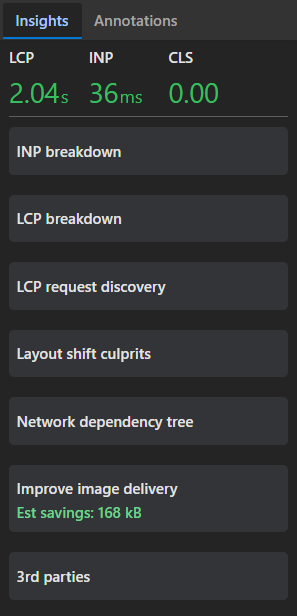
\includegraphics[width=0.55\textwidth]{Images/testing/devtool.png}
    \caption{Kết quả phân tích hiệu suất bằng Chrome DevTools}
    \label{fig:devtools-performance}
\end{figure}

\begin{table}[H]
\centering
\caption{Kết quả đo hiệu suất bằng Chrome DevTools}
\begin{tabularx}{\textwidth}{|p{0.18\textwidth}|p{0.18\textwidth}|X|}
\hline
\textbf{Chỉ số} & \textbf{Kết quả} & \textbf{Nhận xét} \\ \hline
LCP & 2.04s & Thời gian hiển thị nội dung lớn nhất ở mức chấp nhận được, tuy nhiên vẫn có thể tối ưu thêm bằng lazy loading và tối ưu ảnh. \\ \hline
INP & 36ms & Thời gian phản hồi tương tác rất tốt, thao tác click và nhập liệu không có độ trễ đáng kể. \\ \hline
CLS & 0.00 & Giao diện ổn định, không ghi nhận hiện tượng dịch chuyển bố cục trong quá trình tải trang. \\ \hline
\end{tabularx}
\end{table}

Kết quả quan sát cho thấy các trang chính đã có cơ chế phân trang hoặc tải dữ liệu theo nhu cầu. Feed, marketplace, notification, scheduled posts và các danh sách quản trị không tải toàn bộ dữ liệu cùng lúc mà gọi API theo trang hoặc theo bộ lọc. Những tài nguyên ảnh phụ thuộc nhiều vào dữ liệu upload và Cloudinary URL, do đó cần tiếp tục tối ưu kích thước ảnh, lazy loading và cache trình duyệt trong các phiên bản sau.

\subsection{Phân tích Lighthouse của Chrome DevTools}

Lighthouse được sử dụng để đánh giá tổng quan chất lượng frontend theo các nhóm chỉ số:

\begin{itemize}
    \item \textbf{Performance}: hiệu năng tải trang, thời gian render và khả năng phản hồi.
    \item \textbf{Accessibility}: khả năng truy cập, contrast, label của form, alt text cho hình ảnh.
    \item \textbf{Best Practices}: cấu hình bảo mật trình duyệt, HTTPS, lỗi console và sử dụng API web an toàn.
    \item \textbf{SEO}: thẻ meta cơ bản, title, mô tả và khả năng crawl với các trang public.
\end{itemize}

\begin{figure}[H]
    \centering
    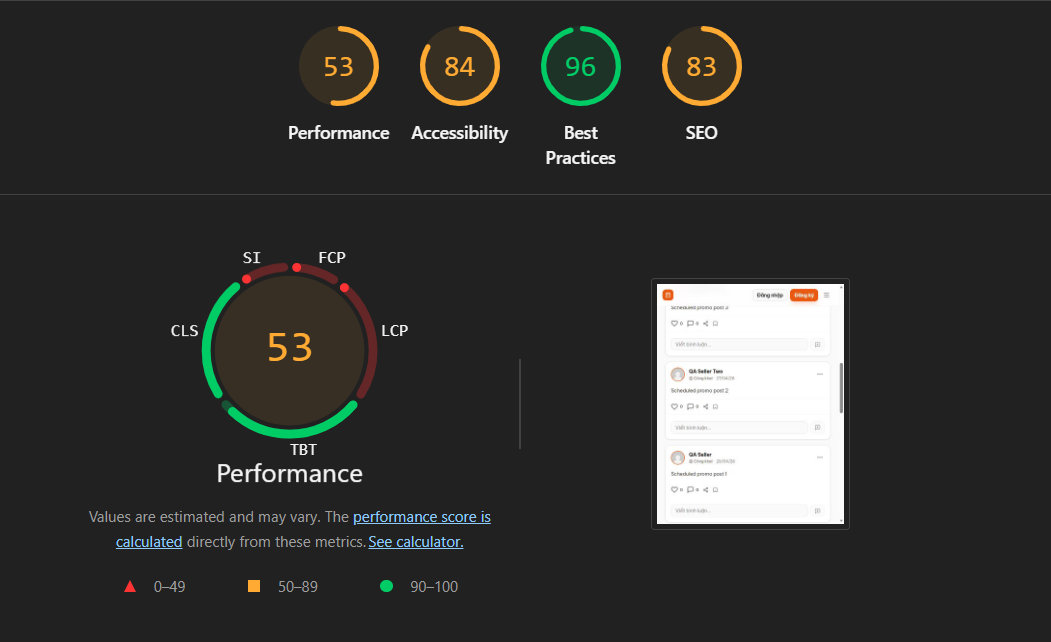
\includegraphics[width=0.95\textwidth]{Images/testing/lighthouse.png}
    \caption{Kết quả phân tích bằng Lighthouse}
    \label{fig:lighthouse-performance}
\end{figure}

\begin{table}[H]
\centering
\caption{Phân tích kết quả Lighthouse theo nhóm chỉ số}
\begin{tabularx}{\textwidth}{|p{0.18\textwidth}|p{0.12\textwidth}|X|p{0.25\textwidth}|}
\hline
\textbf{Nhóm chỉ số} & \textbf{Điểm} & \textbf{Nhận xét} & \textbf{Hướng cải thiện} \\ \hline
Performance & 53 & Điểm hiệu năng ở mức trung bình. Trang có nhiều component, dữ liệu động và media nên thời gian tải/render còn bị ảnh hưởng. & Tối ưu bundle, lazy load component, nén ảnh, dùng skeleton loading, cache hợp lý và giảm JavaScript không cần thiết. \\ \hline
Accessibility & 84 & Khả năng truy cập ở mức khá. Các form chính như login, register, OTP, checkout và seller form đã có label/placeholder cơ bản. & Rà soát thêm aria-label cho icon button, trạng thái lỗi form và contrast ở dark mode. \\ \hline
Best Practices & 96 & Điểm best practices tốt, cho thấy frontend và backend đã đáp ứng phần lớn khuyến nghị cơ bản về triển khai web. & Tiếp tục kiểm tra console warning, cấu hình HTTPS production và kiểm soát mixed content. \\ \hline
SEO & 83 & SEO ở mức khá đối với các trang public như feed, marketplace và product detail. & Bổ sung meta title/description động cho product detail, seller profile và post detail. \\ \hline
\end{tabularx}
\end{table}

Nhìn chung, kết quả kiểm thử hiệu suất cho thấy hệ thống đáp ứng được nhu cầu sử dụng trong phạm vi đồ án. Tuy nhiên, khi dữ liệu tăng lớn hoặc triển khai production với lượng truy cập cao, hệ thống cần tiếp tục được kiểm thử bằng các công cụ chuyên dụng hơn như k6, JMeter hoặc Artillery để đo throughput, latency theo percentiles và khả năng chịu tải của backend API.



\clearpage

\chapter{Triển khai hệ thống}

Chương này mô tả cách đưa Social Commerce lên môi trường thực tế. Hình~\ref{fig:deploy-chapter-overview} tóm tắt kiến trúc triển khai; bản mô tả chi tiết các lớp thành phần nằm ở chương Thiết kế (Hình~\ref{fig:deployment-diagram}).

\begin{itemize}
    \item \textbf{Frontend}: Vercel (Vite + React + TypeScript).
    \item \textbf{Backend}: Amazon EC2 (Node.js, Express, Socket.IO).
    \item \textbf{Cơ sở dữ liệu}: Neon (PostgreSQL, Prisma).
    \item \textbf{Cache}: Redis (ví dụ Upstash hoặc AWS ElastiCache).
\end{itemize}

\begin{figure}[H]
\centering
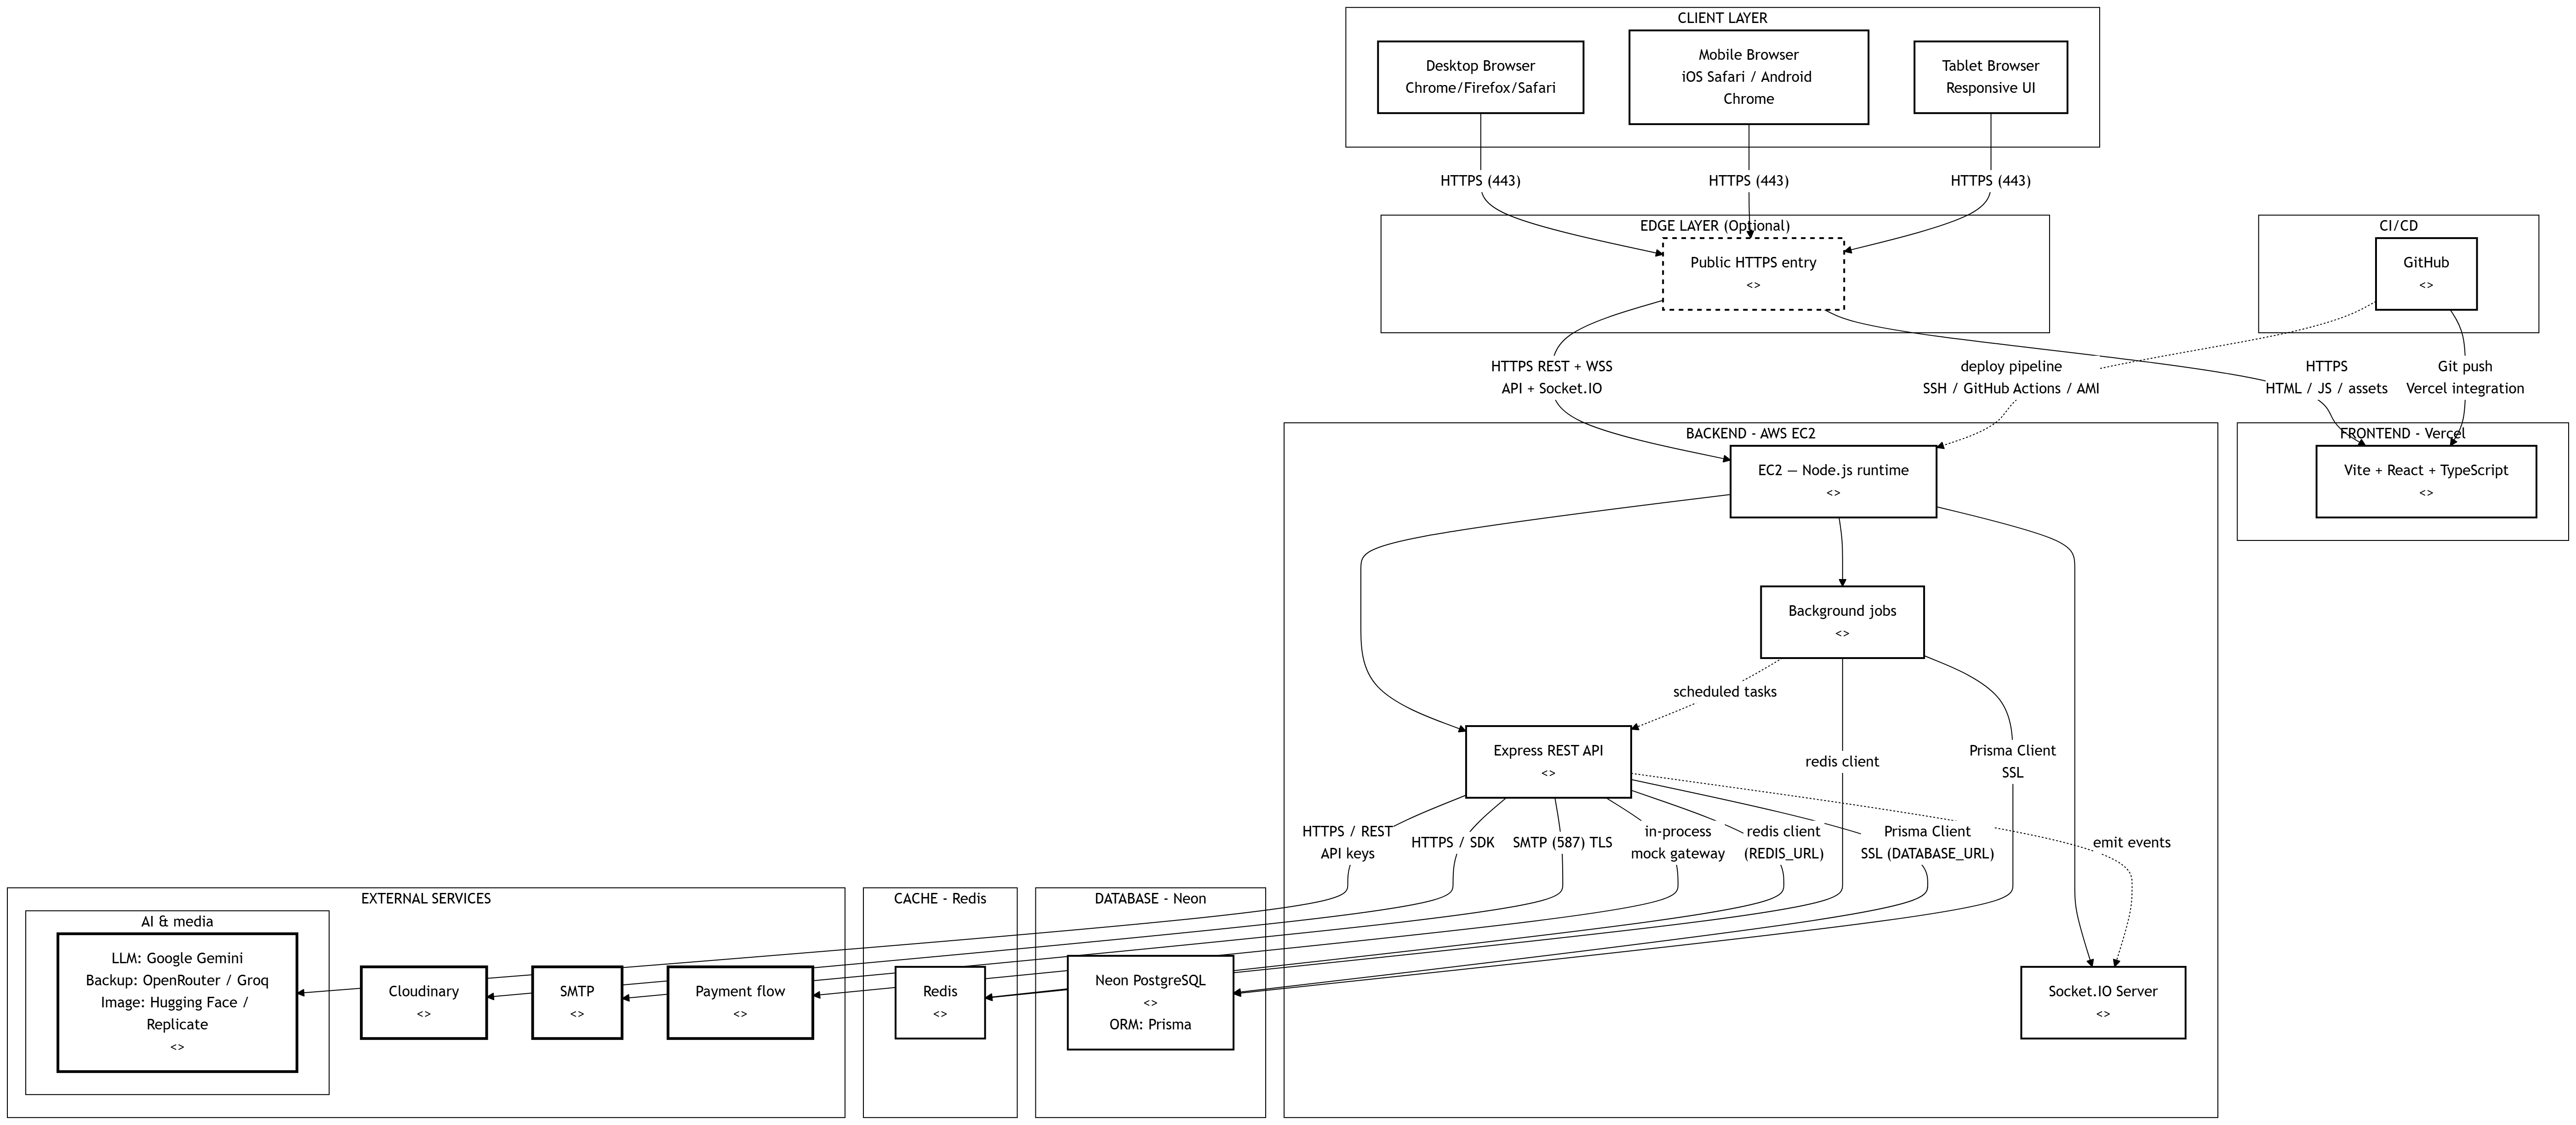
\includegraphics[width=\textwidth]{Images/Deployment Diagram.png}
\caption{Tổng quan kiến trúc triển khai (client, edge, Vercel, EC2, Neon, Redis, dịch vụ ngoài).}
\label{fig:deploy-chapter-overview}
\end{figure}


%----------------------------------------------------------------------
\section{Triển khai cơ sở dữ liệu (Neon) và Redis}
%----------------------------------------------------------------------

\textit{Nên có \texttt{DATABASE\_URL} và \texttt{REDIS\_URL} trước khi cấu hình \texttt{.env} trên EC2.}

\subsection{Neon --- PostgreSQL}

\begin{itemize}
    \item Đăng ký / đăng nhập \href{https://neon.tech}{neon.tech}.
    \item Tạo \textbf{Project} và database mặc định.
    \item Sao chép \textbf{connection string} (PostgreSQL, có SSL) $\rightarrow$ dán vào \texttt{DATABASE\_URL} trong \texttt{backend/.env}.
    \item Trên máy có mạng tới Neon: \texttt{cd backend} $\rightarrow$ \texttt{npm run prisma:generate} $\rightarrow$ \texttt{npm run prisma:migrate:deploy}.
    \item Kiểm tra: Neon SQL Editor hoặc \texttt{npm run prisma:studio} (môi trường dev).
    \item (Tùy chọn) \texttt{npm run prisma:seed} trên môi trường an toàn.
\end{itemize}



\subsection{Redis (cache)}

\begin{itemize}
    \item Tạo database Redis (ví dụ \textbf{Upstash}: copy URL dạng \texttt{rediss://...}; hoặc \textbf{ElastiCache} trong AWS).
    \item Gán \texttt{REDIS\_URL} trong \texttt{backend/.env}.
    \item Khởi động lại tiến trình API (PM2) sau khi đổi biến.
\end{itemize}



%----------------------------------------------------------------------
\section{Triển khai back-end trên Amazon EC2}
%----------------------------------------------------------------------

Stack: \textbf{Ubuntu + Node.js + PM2}; tùy chọn \textbf{Nginx + Certbot} (HTTPS, proxy tới cổng app).

\subsection{Tạo instance EC2}

\begin{itemize}
    \item AWS Console $\rightarrow$ EC2 $\rightarrow$ \textit{Launch instance}.
    \item Chọn AMI \textbf{Ubuntu Server LTS} (x86\_64 hoặc Arm theo instance type).
    \item Chọn instance type (ví dụ \texttt{t3.micro} / \texttt{t2.micro} nếu dùng free tier --- lưu ý giới hạn giờ).
    \item Tạo hoặc chọn \textbf{key pair} (\texttt{.pem}); giữ file private key an toàn.
    \item \textbf{Security group}: mở \textbf{22} (SSH, nên giới hạn IP nếu được), \textbf{80}, \textbf{443} cho HTTP/HTTPS từ Internet (Nginx chấm dứt TLS, proxy về app nội bộ).
    \item Bật \textit{Auto-assign public IP} nếu cần truy cập từ Internet.
    \item Ghi lại \textbf{Public IPv4} hoặc public DNS.
\end{itemize}


\subsection{SSH và cài đặt máy chủ}

\begin{itemize}
    \item Từ máy dev, SSH vào instance (Windows: PowerShell / WSL / Terminal có sẵn \texttt{ssh}).
    \item Ví dụ lệnh (đổi đường key và host):
\begin{lstlisting}[language=bash]
ssh -i "/duong/den/khoa.pem" ubuntu@ec2-xx-xx-xx-xx.ap-southeast-1.compute.amazonaws.com
\end{lstlisting}
    \item Trên server: \texttt{sudo apt update}; cài \texttt{git}.
    \item Cài \textbf{Node.js LTS} (nvm hoặc NodeSource).
    \item Cài PM2: \texttt{sudo npm install -g pm2}.
    \item (Khuyến nghị) Cài \textbf{Nginx} + \textbf{Certbot} $\rightarrow$ chứng chỉ Let's Encrypt cho subdomain \texttt{api.*}; proxy \texttt{443} $\rightarrow$ \texttt{http://127.0.0.1:5000} và bật nâng cấp WebSocket cho Socket.IO.
\end{itemize}

\begin{figure}[H]
\centering
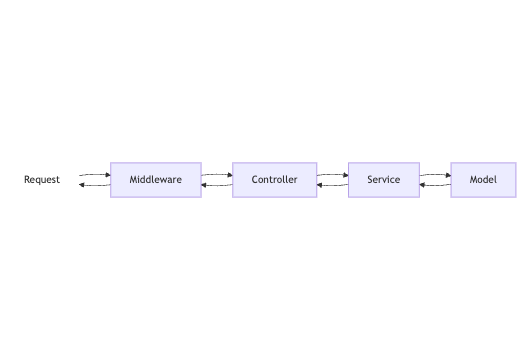
\includegraphics[width=0.88\textwidth]{Images/MVCS.png}
\caption{Minh họa kiến trúc phía máy chủ (MVCS) sau khi SSH và triển khai mã nguồn backend trên EC2.}
\label{fig:deploy-ec2-ssh}
\end{figure}

\subsection{Clone mã nguồn, Prisma, chạy API}

\begin{itemize}
    \item \texttt{git clone} kho SoCo-DATN (monorepo).
    \item \texttt{cd database \&\& npm install}; \texttt{cd ../backend \&\& npm install}.
    \item Tạo \texttt{backend/.env}: \texttt{DATABASE\_URL}, \texttt{REDIS\_URL}, \texttt{JWT\_SECRET}, \texttt{SENSITIVE\_DATA\_KEY}, \texttt{FRONTEND\_URL} (sau có URL Vercel), Cloudinary/SMTP/AI nếu cần.
    \item Chạy:
\begin{lstlisting}[language=bash]
cd backend
npm run prisma:generate
npm run prisma:migrate:deploy
NODE_ENV=production pm2 start src/server.js --name soco-api
pm2 save
pm2 startup
\end{lstlisting}
    \item Sau khi có URL API HTTPS: dùng \texttt{https://.../api} cho \texttt{VITE\_API\_BASE\_URL} trên Vercel; cập nhật \texttt{FRONTEND\_URL} trên server $\rightarrow$ \texttt{pm2 restart soco-api}.
\end{itemize}

%----------------------------------------------------------------------
\section{Triển khai front-end trên Vercel}
%----------------------------------------------------------------------

\subsection{Cấu hình project}

\begin{itemize}
    \item Đăng nhập \href{https://vercel.com}{vercel.com} (thường qua GitHub).
    \item \textit{Add New $\rightarrow$ Project} $\rightarrow$ import repo chứa SoCo-DATN.
    \item \textbf{Root Directory}: chọn \texttt{frontend}.
    \item \textbf{Build Command}: \texttt{npm run build}.
    \item \textbf{Output Directory}: \texttt{dist}.
    \item \textbf{Install Command}: \texttt{npm install} (hoặc \texttt{npm ci} nếu nhóm dùng lockfile thống nhất).
\end{itemize}





\subsection{Biến môi trường và deploy}

\begin{itemize}
    \item \textit{Settings $\rightarrow$ Environment Variables}: thêm \texttt{VITE\_API\_BASE\_URL} = URL API HTTPS có \texttt{/api}.
    \item \textit{Deploy}; khi xong, copy URL dạng \texttt{https://<ten>.vercel.app}.
    \item Cập nhật \texttt{FRONTEND\_URL} trên EC2 khớp URL Vercel (hoặc domain custom) $\rightarrow$ restart PM2.
    \item Push lên nhánh đã liên kết $\rightarrow$ Vercel có thể tự build lại (xem tab Deployments).
\end{itemize}



\begin{figure}[H]
\centering
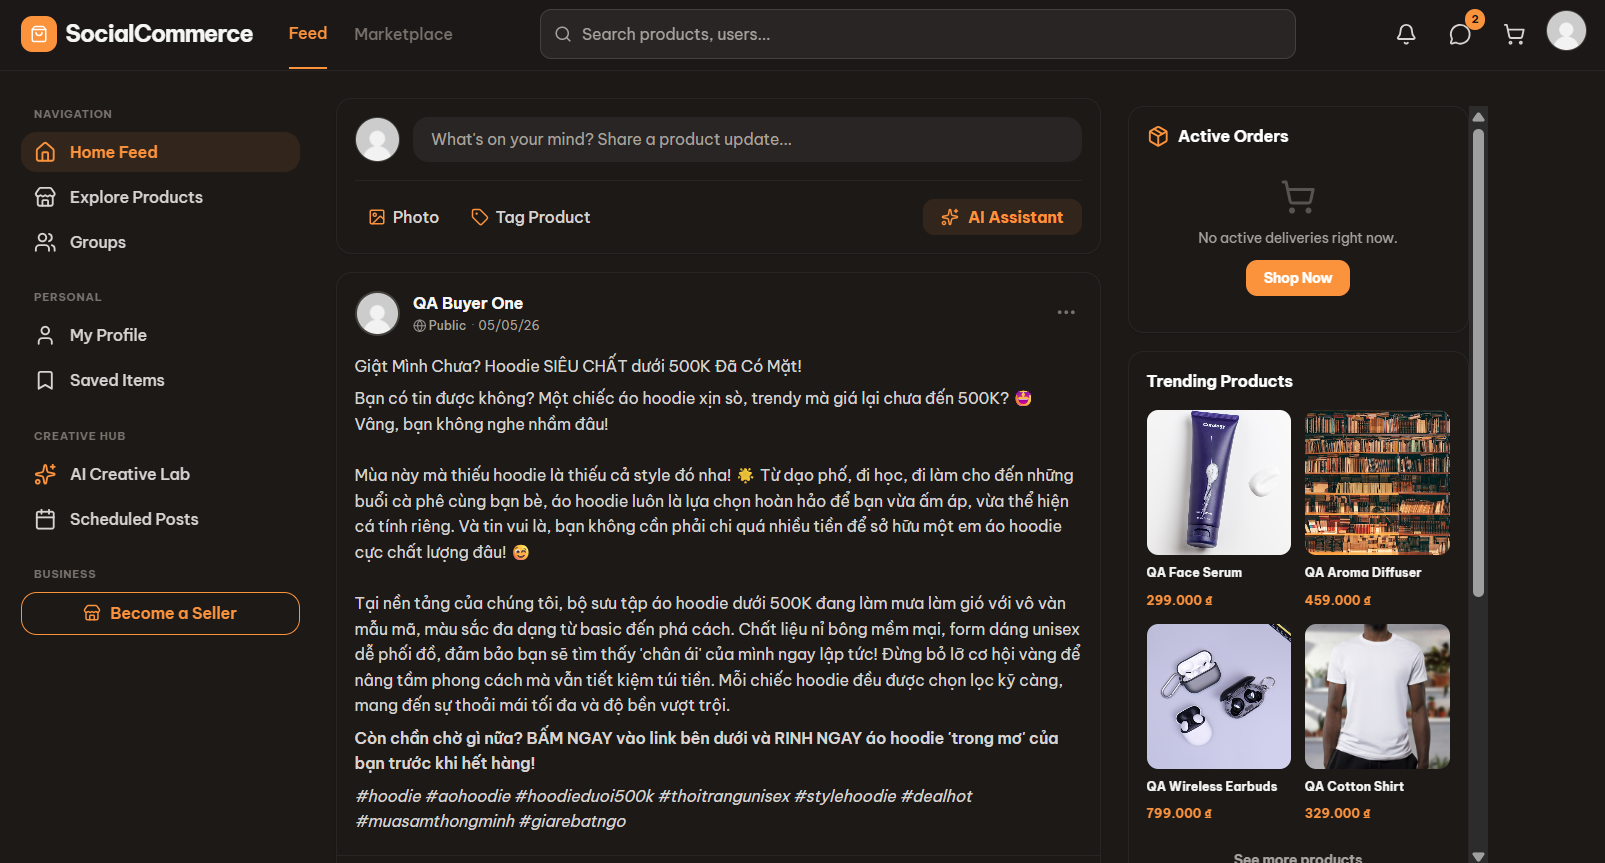
\includegraphics[width=\textwidth]{Images/UI/module2/home-feed.png}
\caption{Minh họa kết quả: giao diện người dùng (bảng tin) sau khi ứng dụng được triển khai và truy cập qua URL công khai.}
\label{fig:deploy-vercel-success}
\end{figure}

%----------------------------------------------------------------------
\section{Backend quản trị và giao diện admin}
%----------------------------------------------------------------------

\begin{itemize}
    \item \textbf{admin/backend}: tiến trình Node riêng (ví dụ PM2 thứ hai), cổng mặc định 5001; \texttt{DATABASE\_URL} trùng Neon; \texttt{ADMIN\_JWT\_SECRET}; \texttt{ADMIN\_CORS\_ORIGIN} khớp origin frontend admin.
    \item \textbf{admin/frontend}: có thể tạo thêm project Vercel, Root \texttt{admin/frontend}; \texttt{VITE\_ADMIN\_API\_BASE\_URL}, \texttt{VITE\_CORE\_PUBLIC\_URL} (xem \texttt{admin/README.md}, \texttt{.env.example}).
\end{itemize}

%----------------------------------------------------------------------
\section{Kết quả và checklist}
%----------------------------------------------------------------------

\subsection{Sau khi hoàn tất}

\begin{itemize}
    \item Mở được SPA từ Vercel; REST và Socket.IO tới EC2 qua HTTPS/WSS.
    \item Dữ liệu trên Neon; Redis hoạt động nếu đã cấu hình.
    \item Ghi vào báo cáo: URL frontend production, URL kiểm tra \texttt{/health} (ví dụ \texttt{https://api.../health}).
\end{itemize}

\subsection{Checklist production}

\begin{itemize}
    \item \texttt{NODE\_ENV=production}; không commit \texttt{.env}.
    \item TLS cho API; \texttt{FRONTEND\_URL} và \texttt{VITE\_*} đúng domain công khai.
    \item Đã chạy migration trên Neon; thử đăng nhập, upload Cloudinary, SMTP, AI (nếu bật).
    \item Rà soát Security Group; hạn chế SSH mở rộng \texttt{0.0.0.0/0} nếu có thể.
\end{itemize}

\clearpage

\chapter{Kết luận}

Đề tài đã xây dựng một hệ thống Social Commerce trên nền tảng web, kết hợp giữa các chức năng mạng xã hội, thương mại điện tử, quản lý người bán và hỗ trợ tạo nội dung bằng AI. Hệ thống hướng đến việc giúp người dùng khám phá sản phẩm thông qua nội dung xã hội, tương tác với người bán, mua hàng trực tiếp trên nền tảng và hỗ trợ seller quản lý hoạt động bán hàng trong một môi trường thống nhất.

\section{Kết quả đạt được}

Sau quá trình phân tích yêu cầu, thiết kế, hiện thực và kiểm thử, hệ thống đã hoàn thành các nhóm chức năng chính sau:

\begin{itemize}
    \item \textbf{Xác thực và quản lý tài khoản}: Hệ thống hỗ trợ đăng ký, đăng nhập, xác thực email, khôi phục mật khẩu, cập nhật hồ sơ và xác thực hai yếu tố. Việc phân quyền giữa buyer, seller và admin được áp dụng ở các API và giao diện tương ứng.
    \item \textbf{Chức năng mạng xã hội}: Người dùng có thể xem feed, tạo bài viết, gắn sản phẩm vào bài viết, thích, bình luận, theo dõi người dùng khác, lưu bài viết/sản phẩm và nhận thông báo real-time.
    \item \textbf{Chức năng thương mại}: Seller có thể tạo và quản lý sản phẩm, hình ảnh, biến thể, tồn kho và trạng thái sản phẩm. Buyer có thể duyệt marketplace, xem chi tiết sản phẩm, thêm vào giỏ hàng, đặt hàng, theo dõi đơn hàng và đánh giá sản phẩm sau mua.
    \item \textbf{Quản lý seller}: Hệ thống hỗ trợ quy trình đăng ký seller, xác minh thông tin, quản lý dữ liệu nhạy cảm, theo dõi dashboard bán hàng, quản lý đơn bán và xử lý các thao tác liên quan đến sản phẩm.
    \item \textbf{Nhắn tin, nhóm và thông báo}: Người dùng có thể tạo hội thoại, gửi tin nhắn, tham gia nhóm cộng đồng, đăng bài trong nhóm và nhận thông báo liên quan đến tương tác xã hội, đơn hàng, tin nhắn và hệ thống.
    \item \textbf{AI hỗ trợ tạo nội dung và tư vấn mua sắm}: Hệ thống tích hợp các API AI để hỗ trợ seller tạo nội dung chữ, caption, hashtag, ý tưởng quảng bá, hình ảnh marketing khi nhà cung cấp AI được cấu hình; đồng thời cung cấp AI Shopping Assistant để người dùng hỏi sản phẩm, so sánh, xem gợi ý và tra cứu đơn hàng.
    \item \textbf{Quản trị hệ thống}: Admin có thể đăng nhập ứng dụng quản trị riêng, xem dashboard tổng quan, quản lý người dùng, sản phẩm, bài viết, danh mục, hồ sơ seller và xử lý báo cáo vi phạm.
    \item \textbf{Kiểm thử}: Các API chính đã được kiểm thử bằng Postman với cả trường hợp thành công và thất bại có chủ đích. Ngoài ra, giao diện cũng được đánh giá ở mức cơ bản thông qua Chrome DevTools và Lighthouse.
\end{itemize}

Về mặt kỹ thuật, hệ thống được triển khai theo kiến trúc tách biệt giữa frontend người dùng, backend core API, frontend admin và backend admin API. Backend sử dụng Node.js, Express.js, Prisma ORM và PostgreSQL; frontend sử dụng React.js, TypeScript và Vite. Kiến trúc này giúp hệ thống dễ bảo trì, tách rõ trách nhiệm giữa các module và thuận lợi cho việc mở rộng trong tương lai.

\section{Hạn chế}

Bên cạnh các kết quả đã đạt được, hệ thống vẫn còn một số hạn chế:

\begin{itemize}
    \item \textbf{Thanh toán và hoàn tiền}: Luồng thanh toán và hoàn tiền hiện chủ yếu được mô phỏng trong phạm vi đồ án, chưa tích hợp cổng thanh toán thực tế như VNPay, MoMo, Stripe hoặc PayPal.
    \item \textbf{Vận chuyển}: Hệ thống chưa tích hợp đơn vị vận chuyển thật để tự động tính phí giao hàng, tạo vận đơn và đồng bộ trạng thái giao hàng.
    \item \textbf{AI phụ thuộc nhà cung cấp bên ngoài}: Chức năng AI phụ thuộc vào API key, quota, tốc độ phản hồi và độ ổn định của nhà cung cấp. Chức năng tạo video bằng AI chưa được triển khai trong phạm vi hiện tại.
    \item \textbf{Kiểm thử tải}: Phần kiểm thử hiệu suất mới dừng ở mức quan sát frontend bằng Chrome DevTools và Lighthouse, chưa có kiểm thử tải chuyên sâu bằng các công cụ như k6, JMeter hoặc Artillery.
    \item \textbf{Tối ưu production}: Một số khía cạnh như logging tập trung, monitoring, alerting, backup tự động, CDN cho media và tối ưu bundle frontend cần được hoàn thiện thêm nếu triển khai ở quy mô lớn.
\end{itemize}

\section{Hướng phát triển}

Trong các phiên bản tiếp theo, hệ thống có thể được mở rộng theo các hướng sau:

\begin{itemize}
    \item Tích hợp cổng thanh toán thật và hoàn thiện quy trình hoàn tiền, đối soát giao dịch.
    \item Kết nối với dịch vụ vận chuyển để hỗ trợ tính phí, tạo vận đơn và theo dõi trạng thái giao hàng tự động.
    \item Cải thiện hệ thống gợi ý sản phẩm và nội dung dựa trên hành vi xem, tìm kiếm, tương tác và lịch sử mua hàng.
    \item Phát triển thêm công cụ phân tích cho seller như hiệu quả bài viết, tỷ lệ chuyển đổi, sản phẩm bán chạy và chân dung khách hàng.
    \item Mở rộng moderation bằng AI để hỗ trợ phát hiện nội dung vi phạm, spam, sản phẩm không phù hợp và báo cáo bất thường.
    \item Tăng cường kiểm thử tự động cho backend, frontend và end-to-end, đồng thời bổ sung kiểm thử tải để đánh giá khả năng chịu tải thực tế.
    \item Hoàn thiện trải nghiệm mobile, tối ưu tốc độ tải trang, lazy loading media, cache tài nguyên và accessibility.
\end{itemize}

\section{Kết luận chung}

Nhìn chung, đề tài đã hoàn thành mục tiêu xây dựng một nền tảng Social Commerce có đầy đủ các chức năng cốt lõi: nội dung xã hội, mua bán sản phẩm, quản lý seller, nhắn tin, thông báo, kiểm duyệt, hỗ trợ tạo nội dung bằng AI và trợ lý mua sắm AI. Hệ thống không chỉ đáp ứng các yêu cầu nghiệp vụ chính của đồ án mà còn tạo nền tảng kỹ thuật rõ ràng để tiếp tục mở rộng trong tương lai.

Thông qua quá trình thực hiện, nhóm đã có cơ hội áp dụng các kiến thức về phân tích yêu cầu, thiết kế hệ thống, thiết kế cơ sở dữ liệu, phát triển REST API, xây dựng giao diện web, tích hợp dịch vụ bên ngoài, xử lý real-time và kiểm thử phần mềm. Đây là cơ sở quan trọng để tiếp tục hoàn thiện sản phẩm theo hướng thực tế hơn, ổn định hơn và phù hợp hơn với nhu cầu vận hành của một nền tảng social commerce hiện đại.

\clearpage

\chapter{Tài liệu tham khảo}

\begin{thebibliography}{99}

\bibitem{react-docs}
React Team. \textit{React Documentation}. Meta Platforms, Inc. \\
\texttt{https://react.dev/}

\bibitem{nodejs-docs}
Node.js Foundation. \textit{Node.js Documentation}. OpenJS Foundation. \\
\texttt{https://nodejs.org/en/docs/}

\bibitem{express-docs}
Express.js Contributors. \textit{Express.js Documentation}. OpenJS Foundation. \\
\texttt{https://expressjs.com/}

\bibitem{postgresql-docs}
PostgreSQL Global Development Group. \textit{PostgreSQL Documentation}. The PostgreSQL Global Development Group. \\
\texttt{https://www.postgresql.org/docs/}

\bibitem{sequelize-docs}
Sequelize Contributors. \textit{Sequelize Documentation}. Sequelize Contributors. \\
\texttt{https://sequelize.org/docs/v6/}

\bibitem{socketio-docs}
Socket.IO Contributors. \textit{Socket.IO Documentation}. Socket.IO Contributors. \\
\texttt{https://socket.io/docs/v4/}

\bibitem{tailwind-docs}
Tailwind Labs. \textit{Tailwind CSS Documentation}. Tailwind Labs, Inc. \\
\texttt{https://tailwindcss.com/docs}

\bibitem{cloudinary-docs}
Cloudinary. \textit{Cloudinary Documentation}. Cloudinary Ltd. \\
\texttt{https://cloudinary.com/documentation}

\bibitem{gemini-api}
Google AI. \textit{Google Gemini API Documentation}. Google LLC. \\
\texttt{https://ai.google.dev/docs}

\bibitem{jwt-rfc}
M. Jones, J. Bradley, N. Sakimura. \textit{JSON Web Token (JWT)}. RFC 7519, May 2015. \\
\texttt{https://tools.ietf.org/html/rfc7519}

\bibitem{bcrypt-paper}
Niels Provos, David Mazières. \textit{A Future-Adaptable Password Scheme}. USENIX Annual Technical Conference, 1999.

\bibitem{rest-api-design}
Leonard Richardson, Mike Amundsen, Sam Ruby. \textit{RESTful Web APIs: Services for a Changing World}. O'Reilly Media, 2013.

\bibitem{social-commerce-survey}
Zhou, L., Zhang, P., \& Zimmermann, H. D. \textit{Social commerce research: An integrated view}. Electronic Commerce Research and Applications, 12(2), 61-68, 2013.

\bibitem{ecommerce-security}
Anderson, R. \textit{Security Engineering: A Guide to Building Dependable Distributed Systems}. Wiley, 3rd Edition, 2020.

\bibitem{websocket-rfc}
I. Fette, A. Melnikov. \textit{The WebSocket Protocol}. RFC 6455, December 2011. \\
\texttt{https://tools.ietf.org/html/rfc6455}

\bibitem{react-patterns}
Michele Bertoli. \textit{React Design Patterns and Best Practices}. Packt Publishing, 2nd Edition, 2019.

\bibitem{nodejs-best-practices}
Yoni Goldberg. \textit{Node.js Best Practices}. GitHub Repository. \\
\texttt{https://github.com/goldbergyoni/nodebestpractices}

\bibitem{postgresql-performance}
Gregory Smith. \textit{PostgreSQL High Performance}. Packt Publishing, 2nd Edition, 2017.

\bibitem{ai-content-generation}
Brown, T., Mann, B., et al. \textit{Language Models are Few-Shot Learners}. Advances in Neural Information Processing Systems, 33, 2020.

\bibitem{real-time-systems}
Kreps, J., Narkhede, N., \& Rao, J. \textit{Kafka: A Distributed Messaging System for Log Processing}. NetDB, 2011.

\bibitem{responsive-design}
Marcotte, E. \textit{Responsive Web Design}. A List Apart, 2010. \\
\texttt{https://alistapart.com/article/responsive-web-design/}

\bibitem{oauth2-rfc}
D. Hardt. \textit{The OAuth 2.0 Authorization Framework}. RFC 6749, October 2012. \\
\texttt{https://tools.ietf.org/html/rfc6749}

\bibitem{https-rfc}
E. Rescorla. \textit{The Transport Layer Security (TLS) Protocol Version 1.3}. RFC 8446, August 2018. \\
\texttt{https://tools.ietf.org/html/rfc8446}

\bibitem{api-design}
Kin Lane. \textit{The API Design Guide}. API Evangelist. \\
\texttt{https://www.apievangelist.com/}

\bibitem{testing-guide}
Kent C. Dodds. \textit{Testing JavaScript}. TestingJavaScript.com. \\
\texttt{https://testingjavascript.com/}

\bibitem{git-workflow}
Vincent Driessen. \textit{A successful Git branching model}. nvie.com, 2010. \\
\texttt{https://nvie.com/posts/a-successful-git-branching-model/}

\bibitem{clean-code}
Martin, R. C. \textit{Clean Code: A Handbook of Agile Software Craftsmanship}. Prentice Hall, 2008.

\bibitem{design-patterns}
Gamma, E., Helm, R., Johnson, R., \& Vlissides, J. \textit{Design Patterns: Elements of Reusable Object-Oriented Software}. Addison-Wesley Professional, 1994.

\bibitem{database-design}
Silberschatz, A., Korth, H. F., \& Sudarshan, S. \textit{Database System Concepts}. McGraw-Hill Education, 7th Edition, 2019.

\bibitem{software-engineering}
Sommerville, I. \textit{Software Engineering}. Pearson, 10th Edition, 2015.

\bibitem{vite-docs}
Vite Contributors. \textit{Vite Documentation}. Vite Contributors. \\
\texttt{https://vitejs.dev/}

\bibitem{shadcn-ui}
shadcn. \textit{shadcn/ui Documentation}. shadcn. \\
\texttt{https://ui.shadcn.com/}

\bibitem{zustand-docs}
Zustand Contributors. \textit{Zustand Documentation}. Zustand Contributors. \\
\texttt{https://zustand-demo.pmnd.rs/}

\bibitem{react-query-docs}
TanStack. \textit{React Query Documentation}. TanStack. \\
\texttt{https://tanstack.com/query/latest}

\bibitem{figma-docs}
Figma Inc. \textit{Figma Documentation}. Figma, Inc. \\
\texttt{https://help.figma.com/}

\bibitem{agile-manifesto}
Beck, K., et al. \textit{Manifesto for Agile Software Development}. agilemanifesto.org, 2001. \\
\texttt{https://agilemanifesto.org/}

\bibitem{scrum-guide}
Schwaber, K., \& Sutherland, J. \textit{The Scrum Guide}. scrumguides.org, 2020. \\
\texttt{https://scrumguides.org/scrum-guide.html}

\end{thebibliography}

\clearpage
\chapter{Phụ lục}

\section{Phân chia công việc}

Phần này trình bày chi tiết về phân chia công việc giữa các thành viên trong nhóm cho giai đoạn 1 của dự án (từ Chương 1 đến Chương 6). Công việc được phân chia một cách công bằng dựa trên khả năng và sở trường của từng thành viên, đồng thời đảm bảo tính hợp tác và hỗ trợ lẫn nhau trong quá trình phát triển dự án.

\begin{longtable}{|p{1cm}|p{3.5cm}|p{10cm}|}
\hline
\textbf{STT} & \textbf{Họ và tên} & \textbf{Công việc} \\
\hline
\endfirsthead

\hline
\textbf{STT} & \textbf{Họ và tên} & \textbf{Công việc} \\
\hline
\endhead

\hline
\endfoot

\hline
\endlastfoot

1 & Trần Hoàng Sơn & 1.1. Viết báo cáo Chương 1: Giới thiệu (động lực phát triển, phạm vi và mục tiêu dự án, cấu trúc báo cáo) \\
& & 2.1.1. Nghiên cứu và phân tích các nền tảng social commerce hiện có (TikTok Shop, Facebook Marketplace) \\
& & 2.1.2. Phân tích các hệ thống quản lý thương mại điện tử để tham khảo \\
& & 3.1.3. Thiết kế Use Case Diagram cho Module 3: Hoạt động Thương mại (Products, Cart, Orders, Reviews) \\
& & 3.2.3. Vẽ Activity Diagram cho các luồng E-commerce (thêm vào giỏ hàng, thanh toán, đánh giá sản phẩm) \\
& & 3.3.3. Thiết kế Sequence Diagram cho các chức năng thương mại (đặt hàng, quản lý đơn hàng) \\
& & 3.4.3. Thiết kế schema database cho các bảng liên quan đến E-commerce (Products, Cart, Orders, Reviews) \\
& & 4.3. Nghiên cứu và so sánh các hệ quản trị cơ sở dữ liệu (PostgreSQL, MySQL, MongoDB) cho Chương 4 \\
& & 5.1.3. Thiết kế giao diện UI/UX trên Figma cho Module 3: Thương mại (trang sản phẩm, giỏ hàng, thanh toán, quản lý đơn hàng) \\
& & 5.2.3. Viết báo cáo Chương 5: Triển khai Hệ thống (phần thiết kế UI/UX Module 3) \\
& & 6.1. Đóng góp vào viết báo cáo Chương 6: Tổng kết và Kế hoạch Tương lai \\
& & 6.2. Review và chỉnh sửa toàn bộ tài liệu báo cáo \\
\hline

2 & Phạm Lê Thanh & 2.1.1. Nghiên cứu và phân tích các nền tảng social commerce hiện có (Instagram Shopping, Pinterest Shopping) \\
& & 2.2. Viết báo cáo Chương 2: Thu thập và Phân tích Yêu cầu (phân tích các hệ thống liên quan, xác định actors và functional requirements) \\
& & 3.1.2. Thiết kế Use Case Diagram cho Module 2: Tương tác Xã hội (Posts, Comments, Follow, Messages, Groups) \\
& & 3.2.2. Vẽ Activity Diagram cho các luồng Social (tạo bài đăng, tương tác, nhắn tin, tham gia nhóm) \\
& & 3.3.2. Thiết kế Sequence Diagram cho các chức năng xã hội (đăng bài, bình luận, theo dõi, chat real-time) \\
& & 3.4.2. Thiết kế schema database cho các bảng liên quan đến Social Features (Posts, Comments, Messages, Notifications) \\
& & 4.1. Nghiên cứu và so sánh các công nghệ Frontend (React, Vue, Angular) cho Chương 4 \\
& & 4.4. Nghiên cứu và so sánh các công nghệ Real-time (Socket.io, WebSocket, Server-Sent Events) cho Chương 4 \\
& & 4.5. Viết báo cáo Chương 4: Nghiên cứu Công nghệ (phần Frontend và Real-time) \\
& & 5.1.2. Thiết kế giao diện UI/UX trên Figma cho Module 2: Tương tác Xã hội (feed, tạo bài đăng, nhắn tin, nhóm) \\
& & 5.1.4. Thiết kế giao diện UI/UX cho Module 6, 7: Lên lịch đăng bài và Hệ thống Thông báo \\
& & 6.1. Đóng góp vào viết báo cáo Chương 6: Tổng kết và Kế hoạch Tương lai \\
\hline

3 & Nguyễn Nhật Tân & 2.1.1. Nghiên cứu và phân tích các nền tảng social commerce hiện có (Shopee, Lazada) \\
& & 2.2.1. Xác định và mô tả chi tiết các Actors (Visitor, User, Buyer, Seller, Admin) cho Chương 2 \\
& & 2.3. Đặc tả các yêu cầu phi chức năng (Performance, Security, Availability, Usability, Scalability, Real-time) cho Chương 2 \\
& & 3.1.1. Thiết kế Use Case Diagram cho Module 1: Quản lý Người dùng và Module 4: Hệ thống Quản trị \\
& & 3.2.1. Vẽ Activity Diagram cho các luồng Authentication (đăng ký, đăng nhập, 2FA, quên mật khẩu) \\
& & 3.3.1. Thiết kế Sequence Diagram cho các chức năng quản trị (quản lý người dùng, kiểm duyệt nội dung, xử lý báo cáo) \\
& & 3.4.1. Thiết kế ERD tổng thể và schema database cho các bảng liên quan đến User Management và Admin \\
& & 3.5. Thiết kế Architecture Diagram tổng thể của hệ thống \\
& & 3.6. Thiết kế Component Diagram và Deployment Diagram \\
& & 3.7. Viết báo cáo Chương 3: Thiết kế Hệ thống (phần Architecture Diagram, Component Diagram, Deployment Diagram) \\
& & 4.2. Nghiên cứu và so sánh các công nghệ Backend (Node.js/Express, Django, Spring Boot) cho Chương 4 \\
& & 4.6. Nghiên cứu và so sánh các công nghệ AI (Google Gemini, OpenAI GPT, Claude) cho Chương 4 \\
& & 5.1.1. Thiết kế giao diện UI/UX trên Figma cho Module 1: Quản lý Người dùng (đăng ký, đăng nhập, profile, settings) \\
& & 5.1.5. Thiết kế giao diện UI/UX trên Figma cho Module 4: Hệ thống Quản trị (dashboard, quản lý người dùng, báo cáo) \\
& & 6.1. Đóng góp vào viết báo cáo Chương 6: Tổng kết và Kế hoạch Tương lai \\
\hline

\end{longtable}

\section{Ghi chú về phân chia công việc}

\begin{itemize}
    \item Công việc được phân chia dựa trên sở trường và khả năng của từng thành viên, đảm bảo tính công bằng và hiệu quả.
    \item Các công việc quan trọng như thiết kế ERD, Architecture Diagram được thực hiện chung để đảm bảo tính nhất quán và chất lượng.
    \item Việc phân chia công việc được điều chỉnh linh hoạt trong quá trình phát triển dự án để đảm bảo tiến độ và chất lượng.
    \item Tất cả các thành viên đều tham gia vào quá trình review và chỉnh sửa để đảm bảo chất lượng tài liệu.
    \item Các module phức tạp được phân chia để tận dụng điểm mạnh của từng thành viên, đồng thời đảm bảo tính hợp tác.
\end{itemize}


\end{document}